\documentclass[aspectratio=169]{beamer}
\usetheme[pageofpages=de,% String used between the current page and the
                         % total page count.
          alternativetitlepage=true,% Use the fancy title page.
          % titlepagelogo=trinity-stacked-full,% Logo for the first page.
          watermark=trinity-stacked,% Watermark used in every page.
          watermarkheight=50px,% Height of the watermark.
          watermarkheightmult=1,% The watermark image is 4 times bigger
                                % than watermarkheight.
          ]{Torino}

% Nouvelle is a green and red alternative to the chameleon color theme.
\setbeamercovered{invisible}
\usecolortheme{nouvelle}%

%--------------------------------------

%Portuguese-specific commands
%--------------------------------------
\usepackage[portuguese]{babel}
%--------------------------------------

%---------------------------------------------------------------------------------
% packages
%---------------------------------------------------------------------------------
\usepackage{verbatim}
\usepackage{preview}
\usepackage{xcolor, soul}
\usepackage[T1]{fontenc}
\usepackage[utf8]{inputenc}
\usepackage{tikz}
\usepackage{listings}
\usepackage{hyperref}
\usepackage{tkz-berge}
\usepackage{tkz-graph}
\usepackage{fancyhdr}
\usepackage{fancyvrb}
\usepackage{graphicx}
\usepackage{amsmath,amssymb,enumerate,ifthen}

% Define um novo ambiente 'mysmallverbatim' que ajusta o tamanho da fonte para 'small'
\DefineVerbatimEnvironment%
{mysmallverbatim}{Verbatim}
{fontsize=\small}
% \usepackage[pdftex]{graphicx}  



\sethlcolor{lightgray}
\newcommand{\mycode}[1]{\textcolor{red}{\hl{\texttt{#1}}}}
% \newcommand{\mycode}[1]{\textcolor{red}{\texttt{#1}}}
\PreviewEnvironment{tikzpicture}

\usetikzlibrary{positioning,shapes.geometric}
\usetikzlibrary{trees,arrows,positioning, calc}

\usetikzlibrary{backgrounds}
\tikzstyle{wv}  =[draw,fill=white, circle,minimum size=18pt,inner sep=0pt, text=black]
\tikzstyle{gv}  =[draw,fill=gray, circle,minimum size=18pt,inner sep=0pt, text=black]
\tikzstyle{rv}  =[draw,fill=red, circle,minimum size=18pt,inner sep=0pt, text=white]
\tikzstyle{bv}  =[draw,fill=black, circle,minimum size=18pt,inner sep=0pt, text=white]
% \tikzstyle{nil} =[draw,isosceles triangle,
% isosceles triangle apex angle=90, draw=black, minimum size=18pt, inner sep=0pt, text=Black]
\tikzstyle{nil} =[draw,rectangle, draw=black, minimum width=0.5em, minimum height=0.5em]
\tikzstyle{db}  =[draw,rectangle, fill=black, minimum width=2em, minimum height=2em]


\usetikzlibrary{trees,arrows,positioning, calc}
% \tikzstyle{brv}  =[draw,fill=red, circle,minimum size=20pt,inner sep=0pt, text=white]
\tikzstyle{brv}  =[draw,fill=red, circle,minimum size=14pt,inner sep=0pt, text=white]
% \tikzstyle{bbv}  =[draw,fill=black, circle,minimum size=20pt,inner sep=0pt, text=white]
\tikzstyle{bbv}  =[draw,fill=black, circle,minimum size=14pt,inner sep=0pt, text=white]
% \tikzstyle{bwv}  =[draw=white,fill=white, circle,minimum size=14pt,inner sep=0pt, text=black]
\tikzstyle{bwv}  =[draw=black,fill=white, rectangle,minimum size=14pt,inner sep=0pt, text=black]

% \tikzstyle{nil} =[draw,isosceles triangle,
% isosceles triangle apex angle=90, draw=black, minimum size=18pt, inner sep=0pt, text=Black]
\tikzstyle{nil} =[fill=black,rectangle, draw=black, minimum width=0.3em, minimum height=0.3em]
\tikzstyle{db}  =[draw,rectangle, fill=black, minimum width=2em, minimum height=2em]
\tikzset{
  treenode/.style = {
    circle, 
    draw=black, 
    align=center, 
    minimum size=1cm
  },
  subtree/.style  = {
    isosceles triangle, 
    draw=black, 
    align=center, 
    minimum height=0.5cm,   
    minimum width=1cm, 
    shape border rotate=90, 
    anchor=north
  }
}


\renewcommand{\chaptername}{Árvore}


\author{Prof. Artur Oliveira}
\institute{Sistemas de Informação - CPAN/UFMS}

% \date{\today} % Date, can be changed to a custom date

\begin{document}

% \begin{frame}
% \titlepage
% \end{frame}


% \title{Rubro Negra}
\date{\today}
\frame{\titlepage}
% \chapter{Árvores Rubro-Negras}
\begin{frame}[fragile] 
  \frametitle{Árvore Rubro-Negra}
  \begin{theorem}
    Uma árvore rubro-negra é uma árvore binária de busca balanceada na 
    qual cada nó interno tem dois filhos. Cada nó interno tem uma cor, 
    tal que:
    
    \begin{itemize}
    \item Árvore balanceada
    \item Trata cada nó como preta ou vermelhos
    \item Cada vez que adicionamos um nó, conferimos a árvore com as regras da ARN.
    \item Dependendo da violação das regras, faremos uma inversão de cores ou rotação para corrigir os erros na árvore
    \end{itemize}
    \end{theorem}
    
    Precisamos adaptar as operações de inserção e deleção de forma que as 
    propriedades rubro negras sejam mantidas.
\end{frame}
    

%%%%%%%%%%%%
%% FRAME %%%
%%%%%%%%%%%%

\begin{frame}[fragile]{Árvore Rubro-Negra - Regras}
  \begin{theorem}
  
  \begin{itemize}
  \item[0.] Cada nó é preto ou vermelho 
  \item[1.] O nó raiz é sempre preto.
  \item[2.] Todos os nós folha (Null) são pretos.
  \item[3.] Novas inserções são sempre vermelhas.  
  \item[4.] Todos os caminhos percorridos na árvore contém o mesmo número de nós pretos (\textbf{\emph{altura-negra}}).
  \item[5.] Nenhum caminho pode ter dois nós vermelhos consecultivos. 
  \item[6.] Se um nó é vermelho, então ambos os filhos são pretos. 
  \item[7.] Os ponteiros dos nós folha (representados como quadrados pretos) continuam sendo "nulos" e não carregam nenhum valor.
  \end{itemize}
  \end{theorem}
  
\end{frame}


\begin{frame}[fragile]

    \begin{figure}[!h]
      \centering
      \caption{Típica árvore rubro-negra} 
    % \begin{preview}
    \begin{tikzpicture}[->,>=stealth',
      % level/.style={sibling distance = 8cm/#1, level distance = 1.5cm},
      level 1/.style={sibling distance=0.4\textwidth, level distance = 0.8cm},
      level 2/.style={sibling distance=0.2\textwidth, level distance = 0.8cm},
      level 3/.style={sibling distance=0.1\textwidth, level distance = 0.8cm},
      level 4/.style={sibling distance=0.05\textwidth, level distance = 0.8cm}]
    \node [bbv] (r){6}
    child {node [brv] {3}
      child {node [bbv] {1}
        child {node [nil] {}}
        child {node [nil] {}}
      }
      child {node [bbv] {5}
        child {node [nil] {}}
        child {node [nil] {}}
      }
    }
    child {node [brv] {8}
      child {node [bbv] {7}
        child {node [nil] {}}
        child {node [nil] {}}
      }
      child {node [bbv] {9}
        child {node [nil] {}}
        child {node [brv] {10}
          child {node [nil] {}}
          child {node [nil] {}}
        }
      }
    }
    ;
  \end{tikzpicture}
  \end{figure}
\end{frame}

%%%%%%%%%%%%
%% FRAME %%%
%%%%%%%%%%%%
\begin{frame}[fragile]
  \frametitle{Regras pra corrigir a árvore}

  \begin{itemize}
    \item \textbf{Tio Preto} - Rotaciona (TPR)
    \item \textbf{Tio Vermelho} - inverte cor (TVI)
  \end{itemize}

\begin{figure}
\begin{minipage}[t]{0.48\linewidth}
\centering
\caption{Resultado da TPR}
\begin{tikzpicture}[->,>=stealth',
  level 1/.style={sibling distance=6em, level distance = 3em},
  level 2/.style={sibling distance=2em, level distance = 3em},
  level 3/.style={sibling distance=1em, level distance = 3em}
]
\node [bbv] (r){c}
    child [color=black] {node [brv] {a}}
    child [color=black] {node [brv] {c}}
;
\end{tikzpicture}
\end{minipage}\hfill
\begin{minipage}[t]{0.48\linewidth}
\caption{Resultado da TVI}
  \begin{tikzpicture}[->,>=stealth',
  level 1/.style={sibling distance=6em, level distance = 3em},
  level 2/.style={sibling distance=2em, level distance = 3em},
  level 3/.style={sibling distance=1em, level distance = 3em}
]
\node [brv] (r){c}
    child [color=black] {node [bbv] {a}}
    child [color=black] {node [bbv] {c}}
;
\end{tikzpicture}
\end{minipage}
\end{figure}
\end{frame}


%%%%%%%%%%%%`'
%% FRAME %%%
%%%%%%%%%%%%

\begin{frame}[fragile]{Caso 1 - O tio de \textbf{a}, (\textbf{d}), é vermelho}
TVC - tio-vermelho-colorir 
Então como a gente faz pra corrigir a quebra de invariante (coloração rubro-negra?) 

É o que vamos ver agora!
\begin{figure}
\begin{minipage}[t]{0.48\linewidth}
\centering
\caption{Antes}
\begin{tikzpicture}[->,>=stealth',
  level 1/.style={sibling distance=6em, level distance = 3em},
  level 2/.style={sibling distance=2em, level distance = 3em},
  level 3/.style={sibling distance=1em, level distance = 3em}
]
\node [bbv] (r){c}
child [color=black] { node [brv] {b}
        child [color=black] {node [bwv] {z}}
        child [color=black] { node [brv] {a}
          child [color=black] {node [bwv] {x}}
          child [color=black] {node [bwv] {y}}
        }
      }
child [color=black] { node [brv] {d}
        child [color=black] {node [bwv] {p}}
        child [color=black] {node [bwv] {q}}
};
\end{tikzpicture}
\end{minipage}\hfill
\begin{minipage}[t]{0.48\linewidth}
\caption{Depois}
  \begin{tikzpicture}[->,>=stealth',
  level 1/.style={sibling distance=6em, level distance = 3em},
  level 2/.style={sibling distance=2em, level distance = 3em},
  level 3/.style={sibling distance=1em, level distance = 3em}
]
\node [brv] (r){c}
child [color=black] { node [bbv] {b}
        child [color=black] {node [bwv] {z}}
        child [color=black] { node [brv] {a}
          child [color=black] {node [bwv] {x}}
          child [color=black] {node [bwv] {y}}
        }
      }
child [color=black] { node [bbv] {d}
        child [color=black] {node [bwv] {p}}
        child [color=black] {node [bwv] {q}}
};
\end{tikzpicture}
\end{minipage}
\end{figure}
\end{frame}

%%%%%%%%%%%%
%% FRAME %%%
%%%%%%%%%%%%

\begin{frame}[fragile]{Caso 2 - O tio de \textbf{a}, (\textbf{d}), é preto e \textbf{a} é filho direito}
TPR - tio-preto-rotaciona
% \pagebreak
\begin{itemize}
  \item Rotação à esquerda do pai de \textbf{a}, (\textbf{b}), ao redor de \textbf{a}
  \item Continua para o \textbf{Caso 3}
\end{itemize}

\begin{columns}[T] % align columns
  \begin{column}{.48\textwidth}
  \rule{\linewidth}{4pt}
  \begin{figure}[!h]
  \caption{Antes}
\begin{tikzpicture}[->,>=stealth',
  % level/.style={sibling distance = 20em, level distance = 3em},
  level 1/.style={sibling distance=6em, level distance = 3em},
  level 2/.style={sibling distance=3em, level distance = 3em},
  level 3/.style={sibling distance=2em, level distance = 3em}
]
\node [bbv] (r){c}
child [color=black] { node [brv] {b}
        child [color=black] {node [bwv] {x}}
        child [color=black] { node [brv] {a}
          child [color=black] {node [bwv] {y}}
          child [color=black] {node [bwv] {z}}
        }
      }
child [color=black] { node [bwv] {w}};
\end{tikzpicture}
\end{figure}
   
\end{column}%
\hfill%
\begin{column}{.48\textwidth}
\rule{\linewidth}{4pt}
      
    
\begin{figure}[!h]
  \centering
  % \centering
  \caption{Depois}
\begin{tikzpicture}[->,>=stealth',
   % level/.style={sibling distance = 20em, level distance = 3em},
   level 1/.style={sibling distance=6em, level distance = 3em},
  level 2/.style={sibling distance=3em, level distance = 3em},
  level 3/.style={sibling distance=2em, level distance = 3em},
  ] 
\node [bbv] (r){c}
child [color=black] { node [brv] {a}
    child [color=black] { node [brv] {b}
      child [color=black] {node [bwv] {x}}
      child [color=black] {node [bwv] {y}}
    }
    child [color=black] {node [bwv] {z}}
}
child [color=black] { node [bwv] {w}};
\end{tikzpicture}
\end{figure}
\end{column}%
\end{columns}
\end{frame}


%%%%%%%%%%%%
%% FRAME %%%
%%%%%%%%%%%%

\begin{frame}[fragile]{Caso 3 - O tio de \textbf{a}, (\textbf{d}), é preto e \textbf{a} é filho esquerdo }

\begin{itemize}
  \item Rotação à direita de \textbf{c}, ao redor de \textbf{b}
  \item Troque as cores entre o pai de \textbf{b}, (\textbf{a}) e seu novo irmão (\textbf{c}).
\end{itemize}
  

\begin{columns}[T] % align columns
  \begin{column}{.31\textwidth}
  \rule{\linewidth}{4pt}
  \begin{figure}[!h]
  \caption{Antes}
\begin{tikzpicture}[->,>=stealth',
  % level/.style={sibling distance = 20em, level distance = 3em},
  level 1/.style={sibling distance=6em, level distance = 3em},
  level 2/.style={sibling distance=3em, level distance = 3em},
  level 3/.style={sibling distance=2em, level distance = 3em}
]
\node [bbv] (r){c}
child [color=black] { node [brv] {a}
    child [color=black] { node [brv] {b}
      child [color=black] {node [bwv] {x}}
      child [color=black] {node [bwv] {y}}
    }
    child [color=black] {node [bwv] {z}}
}
child [color=black] { node [bwv] {w}};
\end{tikzpicture}
\end{figure}
   
\end{column}%
\hfill%
\begin{column}{.31\textwidth}
\rule{\linewidth}{4pt}
      
    
\begin{figure}[!h]
  \centering
  % \centering
  \caption{Durante}
\begin{tikzpicture}[->,>=stealth',
   % level/.style={sibling distance = 20em, level distance = 3em},
   level 1/.style={sibling distance=6em, level distance = 3em},
  level 2/.style={sibling distance=3em, level distance = 3em},
  level 3/.style={sibling distance=3em, level distance = 3em},
  ] 
  \node [brv] (r){a}
  child [color=black] { node [brv] {b}
    child [color=black] {node [bwv] {x}}
    child [color=black] {node [bwv] {y}}
  }
  child [color=black] { node [bbv] {c}
    child [color=black] {node [bwv] {z}}
    child [color=black] {node [bwv] {w}}
  };
\end{tikzpicture}
\end{figure}
\end{column}%
%
\hfill%
\begin{column}{.31\textwidth}
\rule{\linewidth}{4pt}
      
    
\begin{figure}[!h]
  \centering
  % \centering
  \caption{Depois}
  \begin{tikzpicture}[->,>=stealth',
    % level/.style={sibling distance = 20em, level distance = 3em},
    level 1/.style={sibling distance=6em, level distance = 3em},
   level 2/.style={sibling distance=3em, level distance = 3em},
   level 3/.style={sibling distance=3em, level distance = 3em},
   ] 
   \node [bbv] (r){a}
   child [color=black] { node [brv] {b}
     child [color=black] {node [bwv] {x}}
     child [color=black] {node [bwv] {y}}
   }
   child [color=black] { node [brv] {c}
     child [color=black] {node [bwv] {z}}
     child [color=black] {node [bwv] {w}}
   };
 \end{tikzpicture}

\end{figure}
\end{column}%
\end{columns}
\end{frame}
  
% \title{Estruturas de Dados: Apresentação da Disciplina}
\date{\today}
\frame{\titlepage}

\begin{frame}
  \frametitle{Ementa da Disciplina}
  Descrição do conteúdo a ser abordado na disciplina. Este conteúdo é importado automaticamente do Plano Pedagógico do Curso (PPC) vigente. Os tópicos principais incluem:
  \begin{itemize}
    \item Tabelas de Dispersão
    \item Árvores Binárias de Busca
    \item Árvores Balanceadas
    \item Busca Digital
    \item Processamento de Cadeias: Busca de Padrão e Compactação de Dados
  \end{itemize}
  Esta ementa é projetada para fornecer uma compreensão fundamental das estruturas de dados essenciais para a computação, com um foco especial em suas aplicações práticas e teóricas.
\end{frame}

\begin{frame}
  \frametitle{Objetivos Gerais}
  A disciplina visa:
  \begin{itemize}
    \item Compreender os fundamentos e a importância das estruturas de dados, enfatizando sua relevância para a eficiência dos algoritmos e o impacto no desempenho de software.
    \item Desenvolver habilidades de análise de complexidade, capacitando os alunos a analisar a complexidade de tempo e espaço de algoritmos associados a diferentes estruturas de dados.
  \end{itemize}
\end{frame}


\begin{frame}
  \frametitle{Objetivos Específicos - Tabelas de Dispersão}
  Os alunos deverão:
  \begin{itemize}
    \item Compreender o conceito, uso e implementação de tabelas de dispersão.
    \item Analisar e aplicar técnicas de tratamento de colisões.
  \end{itemize}
\end{frame}


\begin{frame}
  \frametitle{Objetivos Específicos - Árvores Binárias de Busca}
  Os alunos deverão:
  \begin{itemize}
    \item Entender a estrutura, propriedades e operações de árvores binárias de busca.
    \item Implementar inserção, busca, remoção e percurso em árvores binárias de busca.
  \end{itemize}
\end{frame}
\begin{frame}
  \frametitle{Objetivos Específicos - Árvores Balanceadas}
  Os alunos deverão:
  \begin{itemize}
    \item Aprender sobre árvores AVL e Red-Black, suas propriedades e operações.
    \item Desenvolver habilidades para implementar e manter árvores balanceadas.
  \end{itemize}
\end{frame}

\begin{frame}
  \frametitle{Objetivos Específicos - Busca Digital}
  Os alunos deverão:
  \begin{itemize}
    \item Entender o princípio da busca digital e sua aplicação em estruturas como Tries.
    \item Implementar árvores de busca digital para otimizar a busca por cadeias de caracteres.
  \end{itemize}
\end{frame}

\begin{frame}
  \frametitle{Objetivos Específicos - Processamento de Cadeias}
  Os alunos deverão:
  \begin{itemize}
    \item Compreender e aplicar algoritmos para busca de padrão em textos.
    \item Estudar e implementar técnicas de compactação de dados.
  \end{itemize}
\end{frame}

\begin{frame}
  \frametitle{Semana 1: Introdução (04/03 - 10/03)}
  \textbf{Objetivos:} Apresentar o curso, objetivos, metodologia e avaliação. Introdução aos conceitos básicos de estruturas de dados.
  
  \textbf{Leitura Recomendada:} Capítulos introdutórios dos livros de Cormen e Ascencio.
\end{frame}

\begin{frame}
  \frametitle{Semana 2: Tabelas de Dispersão (11/03 - 17/03)}
  \textbf{Tópicos:} Conceitos básicos, funções hash, tratamento de colisões.
  
  \textbf{Prática:} Exercícios de implementação de funções hash simples.
\end{frame}

\begin{frame}
  \frametitle{Semana 3: Listas, Filas, Pilhas (18/03 - 24/03)}
  \textbf{Tópicos:} Estrutura de uma lista, e os métodos de busca, inserção e remoção.
  
  \textbf{Prática:} Implementação de listas, filas e pilhas, e reuso de funções.
\end{frame}

\begin{frame}
  \frametitle{Semana 4: Árvores Binárias de Busca - Parte 1 (25/03 - 31/03)}
  \textbf{Tópicos:} Conceitos, inserção, busca e percurso.
  
  \textbf{Prática:} Implementação de árvores binárias de busca.
\end{frame}

\begin{frame}
  \frametitle{Semana 5: Árvores Binárias de Busca - Parte 2 (01/04 - 07/04)}
  \textbf{Tópicos:} Remoção, propriedades e aplicações práticas.
  
  \textbf{Prática:} Exercícios de complexidade e otimização.
\end{frame}

\begin{frame}
  \frametitle{Semana 6: Árvores Balanceadas - AVL (08/04 - 14/04)}
  \textbf{Tópicos:} Introdução, rotações, inserção e remoção.
  
  \textbf{Prática:} Implementação de árvores AVL.
\end{frame}

\begin{frame}
  \frametitle{Semana 7: Árvores Balanceadas - Red-Black (15/04 - 21/04)}
  \textbf{Tópicos:} Conceitos, propriedades, operações.
  
  \textbf{Prática:} Implementação de árvores Red-Black.
\end{frame}

\begin{frame}
  \frametitle{Semana 8: Busca Digital (22/04 - 28/04)}
  \textbf{Tópicos:} Trie, operações básicas, aplicabilidade.
  
  \textbf{Prática:} Implementação de Tries para busca de padrões.
\end{frame}

\begin{frame}
  \frametitle{Semana 9: Revisão e Avaliação Intermediária (29/04 - 05/05)}
  \textbf{Atividades:} Primeira prova teórica/prática.
\end{frame}

\begin{frame}
  \frametitle{Semana 10: Processamento de Cadeias - Busca de Padrão (06/05 - 12/05)}
  \textbf{Tópicos:} Algoritmos de busca de padrões, KMP, Boyer-Moore.
  
  \textbf{Prática:} Implementação e análise de algoritmos de busca.
\end{frame}

\begin{frame}
  \frametitle{Semana 11: Processamento de Cadeias - Compactação de Dados (13/05 - 19/05)}
  \textbf{Tópicos:} Técnicas de compactação, Huffman, LZW.
  
  \textbf{Prática:} Implementação de algoritmos de compactação.
\end{frame}

\begin{frame}
  \frametitle{Semana 12-13: Projetos Práticos (20/05 - 02/06)}
  \textbf{Atividades:} Desenvolvimento de projetos práticos em pequenos grupos, aplicando as estruturas de dados estudadas.
\end{frame}

\begin{frame}
  \frametitle{Semana 14: Aplicações Avançadas e Estudo de Caso (03/06 - 09/06)}
  \textbf{Tópicos:} Discussão de estudos de caso, uso de estruturas de dados em sistemas reais.
\end{frame}

\begin{frame}
  \frametitle{Semana 15: Revisão Geral (10/06 - 16/06)}
  \textbf{Atividades:} Revisão de todos os tópicos, sessões de dúvidas.
\end{frame}

\begin{frame}
  \frametitle{Semana 16-17: Apresentação dos Projetos Práticos (17/06 - 30/06)}
  \textbf{Atividades:} Apresentação e avaliação dos projetos práticos. Feedback individual e em grupo.
\end{frame}

\begin{frame}
  \frametitle{Semana 18: Avaliação Final e Encerramento (01/07 - 05/07)}
  \textbf{Atividades:} Avaliação final teórica. Encerramento do curso, feedback e discussão sobre aprendizados.
\end{frame}
\begin{frame}
  \frametitle{Metodologia da Disciplina}
  A disciplina será conduzida através de:
  \begin{itemize}
    \item Aulas Expositivas: Utilização do quadro e giz, e projetor para explicar conceitos, desenhar estruturas e demonstrar algoritmos.
    \item Práticas de Programação: Exercícios em sala de aula e laboratório de computação para aplicação prática dos conceitos.
  \end{itemize}
\end{frame}
\begin{frame}
  \frametitle{Estudo de Casos e Projetos Práticos}
  A disciplina incluirá:
  \begin{itemize}
    \item Análise de Casos Reais: Discussão sobre a aplicação de estruturas de dados em problemas reais.
    \item Desenvolvimento de Projetos: Trabalho em projetos práticos em grupos para solucionar desafios complexos.
  \end{itemize}
\end{frame}
\begin{frame}
  \frametitle{Avaliação e Feedback}
  Para promover o aprendizado efetivo, será aplicado:
  \begin{itemize}
    \item Avaliações Contínuas: Quizzes, exercícios de programação e participação.
    \item Feedback Construtivo: Orientações individuais e em grupo sobre as atividades.
  \end{itemize}
\end{frame}
\begin{frame}
  \frametitle{Recursos Complementares}
  Para aprofundamento do conhecimento:
  \begin{itemize}
    \item Materiais Online e Leituras Adicionais: Artigos, tutoriais, fóruns, além das leituras dos livros-texto.
  \end{itemize}
\end{frame}
\begin{frame}
  \frametitle{Bibliografia Básica}
  Livros essenciais para o estudo da disciplina:
  \begin{itemize}
    \item ASCENCIO, Ana Fernanda Gomes. \emph{Estruturas de dados: algoritmos, análise da complexidade e implementações em Java e C/C++}. São Paulo, SP: Pearson, 2010-2012. ISBN 978-85-7605-881-6.
    \item CORMEN, Thomas H. \emph{Algoritmos: teoria e prática}. Rio de Janeiro, RJ: Elsevier, 2012. ISBN 978-85-352-3699-6.
    \item EDMONDS, J. \emph{How to Think About Algorithms}. 1.ed. Cambridge: Cambridge University Press, 2008. ISBN: 978-0521614108.
  \end{itemize}
\end{frame}
\begin{frame}
  \frametitle{Bibliografia Complementar}
  Leituras adicionais para aprofundamento:
  \begin{itemize}
    \item DEITEL, Harvey M.; DEITEL, P. J. \emph{C++: como programar}. 5. ed. Porto Alegre, RS: Bookman, 2006. ISBN 85-7307-740-9.
    \item GUSFIELD, D. \emph{Algorithms on strings trees and sequences}. Cambridge: Cambridge University Press, 1997. ASIN: B009NG2XWA.
    \item KLEINBERG, Jon; TARDOS, Éva. \emph{Algorithm design}. Boston, MA: Pearson, c2014. ISBN 0321295358.
  \end{itemize}
\end{frame}

% \title{Introdução às Tabelas de Dispersão}
\date{\today}
\frame{\titlepage}

% Slide 1: Introdução às Tabelas de Dispersão
% Slide de Introdução às Tabelas de Dispersão
% Definição e Propósito: A definição e o propósito estão bem explicados. Considerar adicionar um exemplo simples de aplicação para ilustrar melhor a utilidade das tabelas de dispersão.
% Importância: O texto está claro, mas poderia ser enriquecido com exemplos específicos de como as tabelas de dispersão contribuem para o desempenho de sistemas em cenários reais.
\begin{frame}[fragile]
  \frametitle{Introdução às Tabelas de Dispersão}
  \begin{itemize}
    \item Definição e propósito das tabelas de dispersão:
      \begin{itemize}
        \item \textbf{Definição:} As tabelas de dispersão são estruturas de dados que mapeiam chaves para valores, permitindo uma recuperação eficiente dos valores associados às chaves.
        \item \textbf{Propósito:} Elas são amplamente utilizadas em diversos campos da ciência da computação e da engenharia de software devido à sua capacidade de armazenar e recuperar dados de forma rápida e eficiente.
      \end{itemize}
  \end{itemize}
\end{frame}

\begin{frame}[fragile]
  \frametitle{Introdução às Tabelas de Dispersão}
  \begin{itemize}
    
    \item Importância no armazenamento e recuperação eficiente de dados:
      \begin{itemize}
        \item Em muitas aplicações, especialmente aquelas que envolvem grandes volumes de dados, como bancos de dados, sistemas de cache e dicionários, as tabelas de dispersão são essenciais para garantir um acesso rápido e eficiente aos dados.
        \item Elas são usadas para resolver problemas como pesquisa, indexação e associação de chaves a valores, proporcionando uma maneira eficiente de armazenar e recuperar informações.
      \end{itemize}
  \end{itemize}
\end{frame}

% Slide 2: Como Funcionam as Tabelas de Dispersão
% Slide de Como Funcionam as Tabelas de Dispersão
% Processo de Mapeamento: Considerar a inclusão de um diagrama para ilustrar o processo de conversão de chaves em índices de tabela.
% Funções Hash: O texto está claro, mas adicionar um exemplo concreto de uma função hash pode ajudar a ilustrar o conceito.
\begin{frame}[fragile]
  \frametitle{Como Funcionam as Tabelas de Dispersão}
  \begin{itemize}
    \item \textbf{Processo de mapeamento de chaves para índices de tabela:}
      \begin{itemize}
        \item Utilizam funções hash para converter chaves em índices de tabela, onde os valores associados são armazenados.
        \item O objetivo é distribuir as chaves uniformemente pela tabela, minimizando colisões e facilitando uma recuperação eficiente.
        \item \textbf{Diagrama:} [Incluir um diagrama aqui que ilustre uma chave sendo convertida em um índice de tabela através de uma função hash, destacando a distribuição uniforme das chaves.]
      \end{itemize}
    
  \end{itemize}
\end{frame}
\begin{frame}[fragile]
  \frametitle{Como Funcionam as Tabelas de Dispersão}
  \begin{figure}
    \centering
    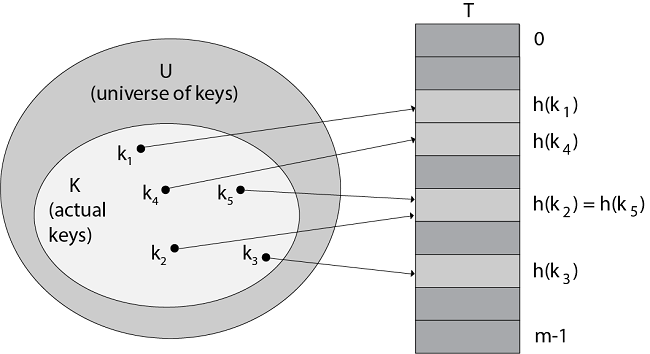
\includegraphics[width=0.8\textwidth]{aulas/aula2-hash-fig1.png}
    \caption{Caption of the Image}
  \end{figure}
\end{frame}
\begin{frame}[fragile]
  \frametitle{Como Funcionam as Tabelas de Dispersão}
  \begin{itemize}
    \item \textbf{Uso de funções hash para conversão de chaves:}
      \begin{itemize}
        \item Essenciais para a eficiência das tabelas de dispersão, as funções hash transformam chaves em índices de tabela de maneira rápida.
        \item Distribuem as chaves uniformemente, evitando colisões excessivas e otimizando o desempenho.
        \item \textbf{Exemplo Concreto:} Suponha uma função hash simples onde a chave é um número inteiro e o tamanho da tabela é 10. A função hash pode ser \(hash(k) = k \mod 10\), onde \(k\) é a chave. Se \(k = 23\), então \(hash(23) = 3\), indicando que o valor associado à chave 23 será armazenado no índice 3 da tabela.
      \end{itemize}
  \end{itemize}
\end{frame}


% Slide 3: Funções Hash
% Slide de Funções Hash
% Definição e Propriedades: A explicação está adequada. Seria útil incluir exemplos visuais para demonstrar a uniformidade e a eficiência.
% Exemplos de Funções Hash: Está bom, mas considerar adicionar exemplos de código ou pseudocódigo para as funções de hash mencionadas.
\begin{frame}[fragile]
  \frametitle{Definição e Propriedades das Funções Hash}
  \begin{itemize}
    \item \textbf{Definição:} 
      \begin{itemize}
        \item Uma função hash converte dados de tamanho variável em valores de 
        tamanho fixo, ideal para índices de tabela.
      \end{itemize}
    \item \textbf{Propriedades desejáveis:}
      \begin{itemize}
        \item \textbf{Uniformidade:} Distribui chaves de forma uniforme, 
        evitando sobrecarga em partes específicas da tabela.
        \item \textbf{Eficiência:} Rápida no cálculo, garantindo acesso ágil 
        aos dados.
        \item \textbf{Baixa probabilidade de colisão:} Minimiza casos onde 
        chaves distintas resultam no mesmo índice.
      \end{itemize}
    \item \textbf{Visualização:} Incluir um gráfico demonstrando a distribuição 
    uniforme das chaves pela tabela pode ajudar a ilustrar a uniformidade. 
    (Considerar adicionar um gráfico ou diagrama que ilustre esta propriedade.)
  \end{itemize}
\end{frame}

\begin{frame}[fragile]
  \frametitle{Exemplos de Funções Hash com Pseudocódigo}
  \begin{itemize}
    \item \textbf{Exemplos de funções hash simples com pseudocódigo:}
      \begin{itemize}
        \item \textbf{Função de Módulo:}
        \begin{mysmallverbatim}
            funcao_hash_modulo(chave, tamanho_da_tabela):
              return chave % tamanho_da_tabela
        \end{mysmallverbatim}
        \item \textbf{Função de Multiplicação:}
          \begin{mysmallverbatim}
            funcao_hash_multiplicacao(chave, tamanho_da_tabela):
              A = 0.6180339887 # constante (número de ouro - 1)
              return floor(tamanho_da_tabela * (chave * A \% 1))
          \end{mysmallverbatim}
      \end{itemize}
    \item Estes pseudocódigos ilustram métodos comuns para transformar chaves 
    em índices de tabela. A função de módulo é simples e direta, enquanto a 
    função de multiplicação utiliza uma constante para ajudar a distribuir as 
    chaves de maneira mais uniforme.
  \end{itemize}
\end{frame}




% Slide 4: Prática - Implementando Funções Hash Simples

\begin{frame}[fragile]
  \frametitle{Prática - Implementando Funções Hash Simples}
  \begin{mysmallverbatim}
    // Exemplo de função hash simples em pseudocódigo
    funcao hash(chave):
      return chave % tamanho_da_tabela
  \end{mysmallverbatim}
  \begin{itemize}
    \item A implementação acima mostra uma função hash simples que calcula o resto da divisão da chave pelo tamanho da tabela.
    \item Esta é uma abordagem comum para implementação de funções hash simples, onde a chave é mapeada diretamente para um índice na tabela.
    \item No entanto, é importante considerar que essa função pode resultar em colisões se as chaves não estiverem uniformemente distribuídas.
    \item Para testar a função hash, é recomendável utilizar uma variedade de chaves e verificar se os índices resultantes estão distribuídos de forma uniforme pela tabela.
    \item Também é importante considerar o desempenho da função hash em diferentes cenários e o impacto das colisões no desempenho geral da tabela de dispersão.
  \end{itemize}
\end{frame}


% Aula 2: Tratamento de Colisões
% Slide 1: Introdução ao Tratamento de Colisões

\begin{frame}[fragile]
  \frametitle{Introdução ao Tratamento de Colisões}
  O que são colisões e por que ocorrem?
      \begin{itemize}
        \item Colisões ocorrem quando duas ou mais chaves diferentes são mapeadas para o mesmo índice na tabela de dispersão.
        \item Elas são inevitáveis em tabelas de dispersão de tamanho fixo, especialmente quando o espaço de chaves é maior do que o número de índices na tabela.
        \item As colisões podem ocorrer devido à natureza das funções hash ou à distribuição desigual das chaves.
      \end{itemize}
\end{frame}

\begin{frame}[fragile]
  \frametitle{Introdução ao Tratamento de Colisões}
  Impacto das colisões no desempenho das tabelas de dispersão:
      \begin{itemize}
        \item Colisões podem causar uma redução significativa no desempenho das tabelas de dispersão, pois aumentam o tempo de busca e inserção de elementos.
        \item Se não forem tratadas adequadamente, as colisões podem levar a uma degradação do desempenho e a uma distribuição desigual dos elementos na tabela.
        \item Portanto, é importante implementar métodos eficazes de tratamento de colisões para garantir um desempenho ótimo das tabelas de dispersão.
      \end{itemize}
\end{frame}


\begin{frame}[fragile]
  \frametitle{Tratamento de Colisões}
  \begin{figure}
    \centering
    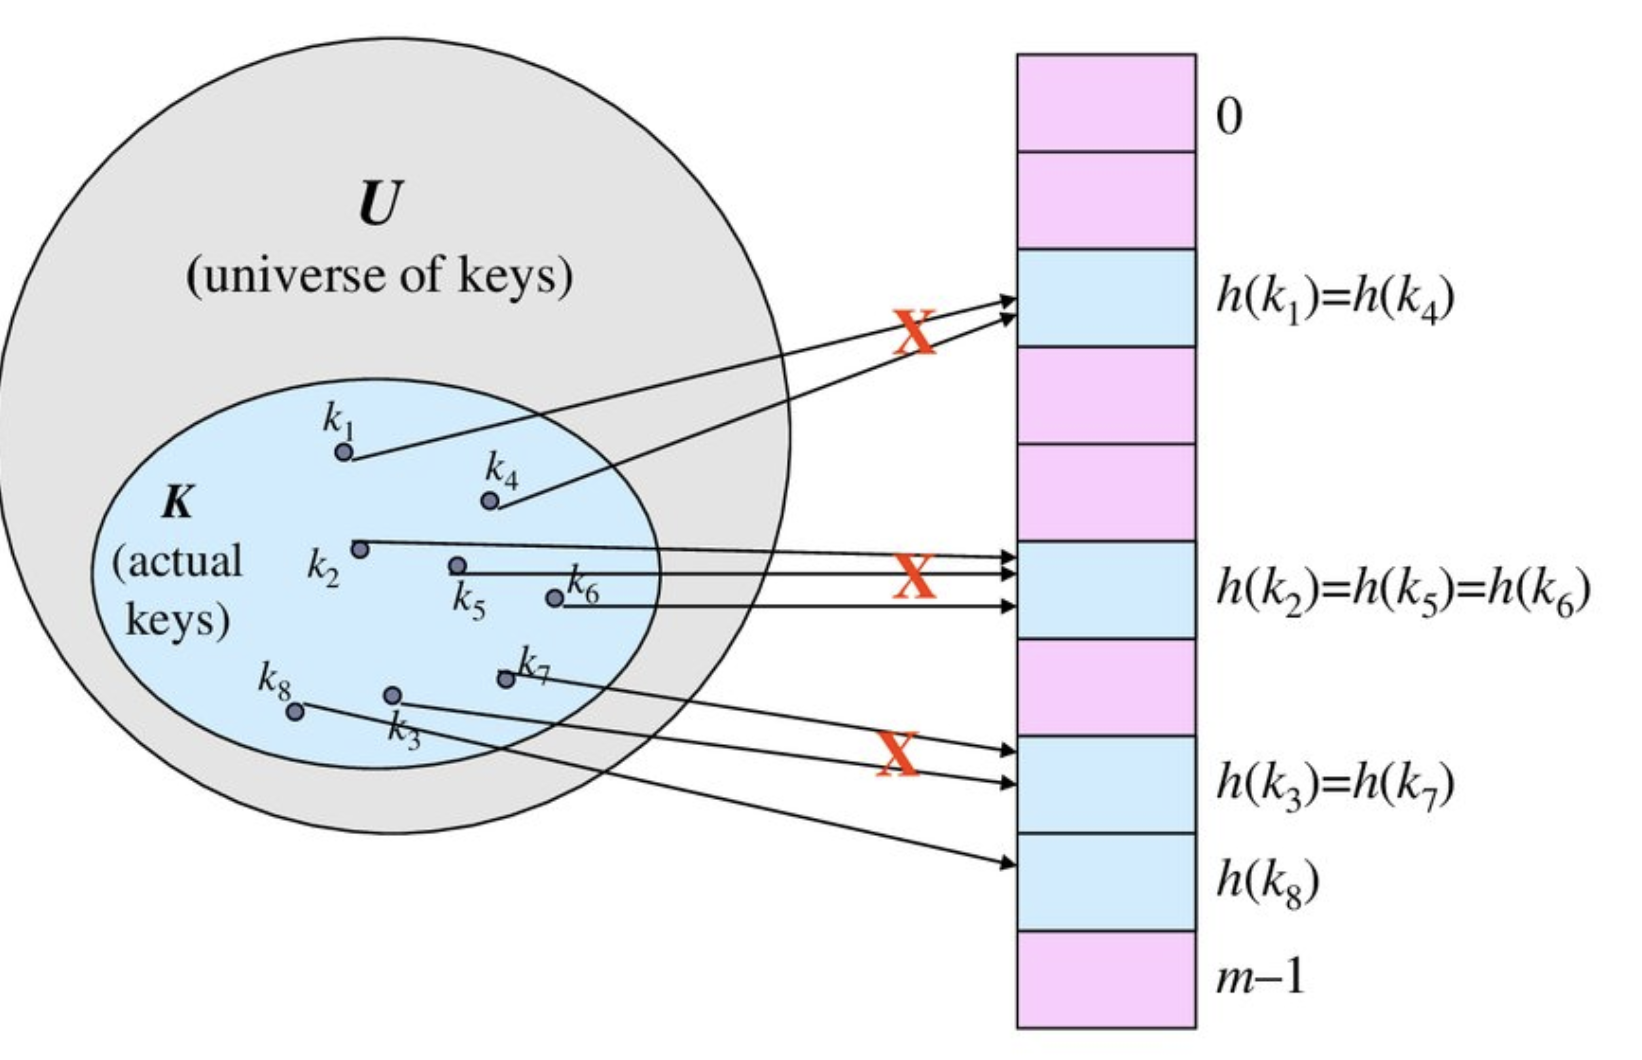
\includegraphics[width=0.8\textwidth]{aulas/aula2-hash-fig2.png}
    \caption{Tratamento de Colisões}
  \end{figure}
\end{frame}

% Slide 2: Métodos de Tratamento de Colisões

\begin{frame}[fragile]
  \frametitle{Métodos de Tratamento de Colisões}
  \begin{itemize}
    \item Encadeamento externo:
      \begin{itemize}
        \item No método de encadeamento externo, cada entrada da tabela de dispersão mantém uma lista encadeada de todos os elementos que colidem naquele índice específico.
        \item Quando ocorre uma colisão, o novo elemento é simplesmente adicionado à lista encadeada correspondente.
        \item Este método é simples de implementar e eficaz para lidar com colisões, especialmente em cenários onde as colisões são frequentes.
        \item No entanto, pode exigir mais espaço de memória devido à necessidade de armazenar as listas encadeadas.
      \end{itemize}
  \end{itemize}
\end{frame}

\begin{frame}[fragile]
  \frametitle{Tratamento de Colisões - Encadeamento}
  \begin{figure}
    \centering
    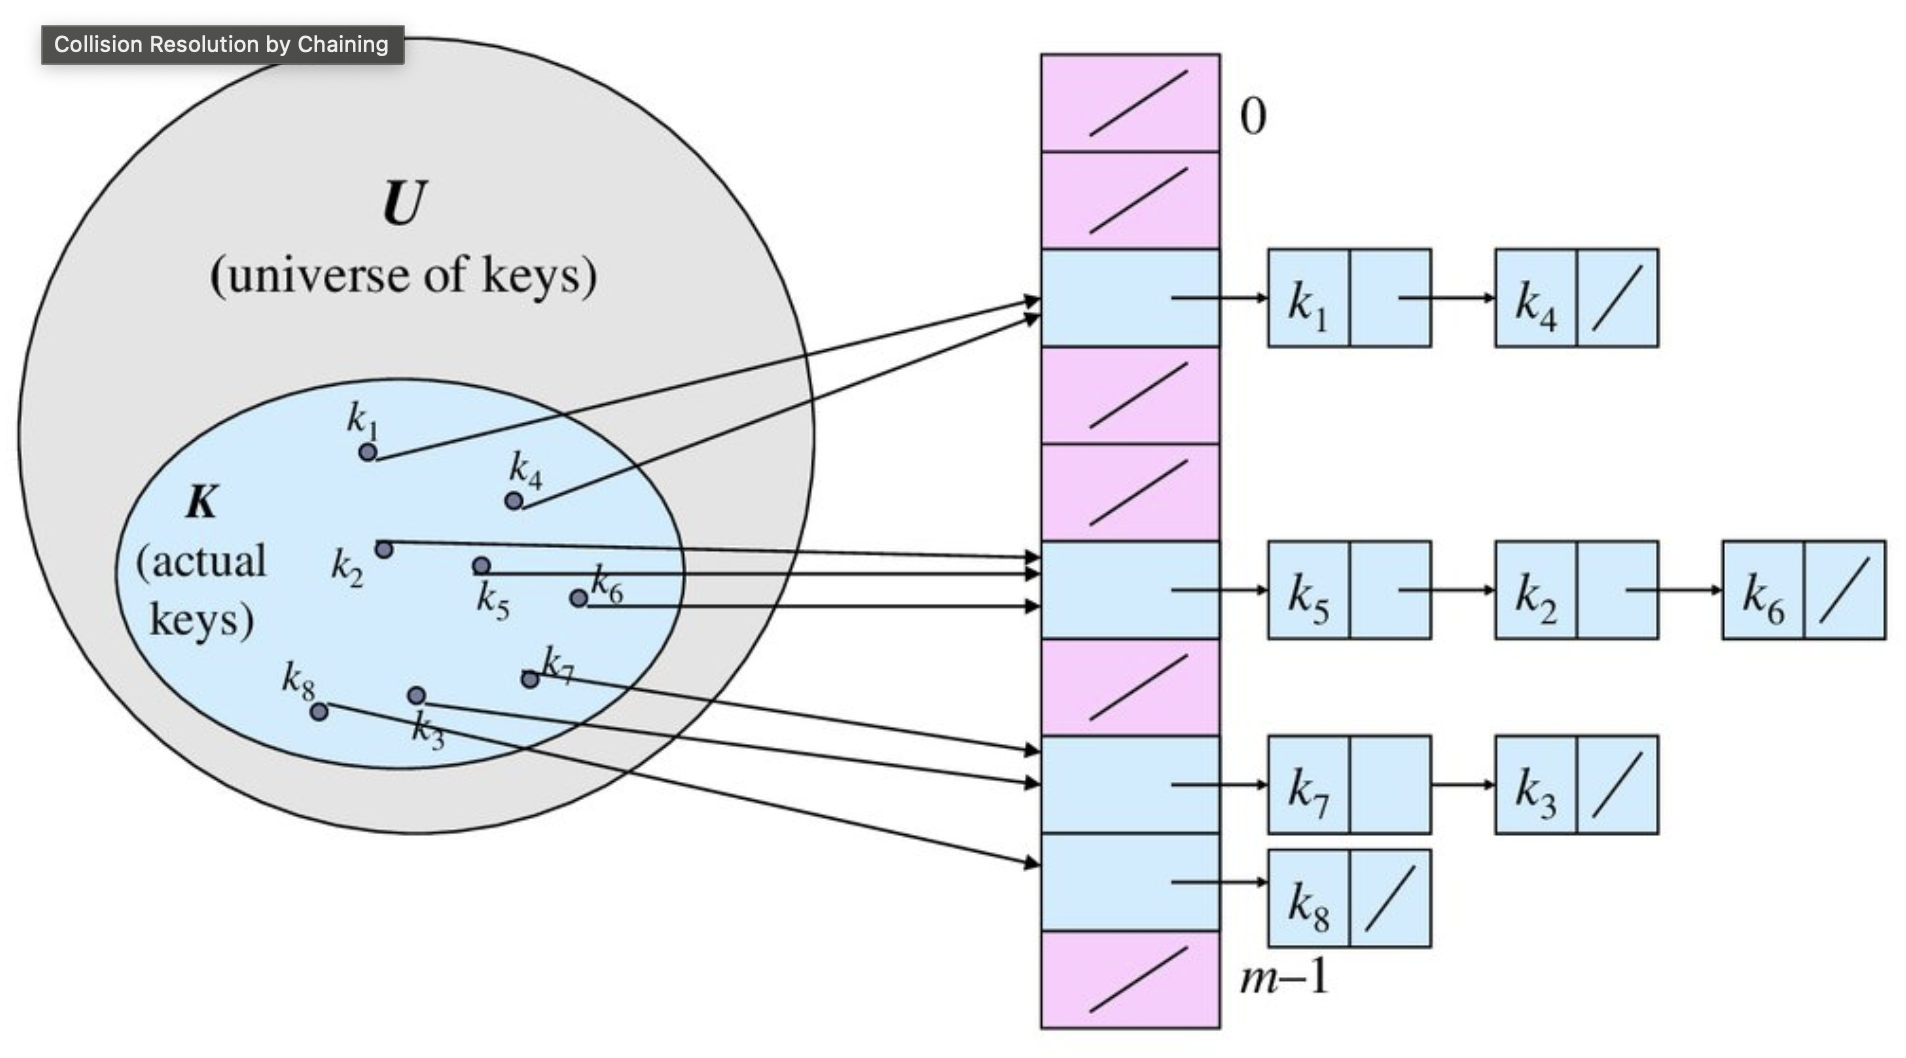
\includegraphics[width=0.8\textwidth]{aulas/aula2-hash-fig3.png}
    \caption{Tratamento de Colisões}
  \end{figure}
\end{frame}


\begin{frame}[fragile]
  \frametitle{Métodos de Tratamento de Colisões}
  \begin{itemize}
    \item Endereçamento aberto:
      \begin{itemize}
        \item O endereçamento aberto é uma abordagem em que, quando ocorre uma colisão, a tabela de dispersão é pesquisada por outra posição livre para inserir o novo elemento.
        \item Existem várias técnicas de endereçamento aberto, incluindo sondagem linear, sondagem quadrática e hashing duplo.
        \item Estas técnicas diferem na forma como procuram por posições alternativas na tabela quando ocorre uma colisão.
        \item O endereçamento aberto pode ser mais eficiente em termos de uso de memória, mas requer cuidados especiais para evitar clusters de colisões.
      \end{itemize}
  \end{itemize}
\end{frame}


% Slide 3: Exemplos e Análise de Métodos de Tratamento de Colisões

\begin{frame}[fragile]
  \frametitle{Exemplos e Análise de Métodos de Tratamento de Colisões}
Comparação dos métodos de tratamento de colisões:
      \begin{itemize}
        \item Encadeamento externo:
          \begin{itemize}
            \item No método de encadeamento externo, as colisões são tratadas armazenando múltiplos elementos que colidem no mesmo índice em uma estrutura de dados separada, como uma lista encadeada.
            \item Vantagens:
              \begin{itemize}
                \item Fácil implementação.
                \item Eficiente para lidar com colisões frequentes.
              \end{itemize}
            \item Desvantagens:
              \begin{itemize}
                \item Pode consumir mais espaço de memória devido à necessidade de armazenar listas encadeadas.
                \item Pode levar a acessos indiretos adicionais durante a busca de elementos.
              \end{itemize}
          \end{itemize}
      \end{itemize}
\end{frame}

\begin{frame}[fragile]
  \frametitle{Exemplos e Análise de Métodos de Tratamento de Colisões (Continuação)}
Comparação dos métodos de tratamento de colisões (cont.):
      \begin{itemize}
        \item Endereçamento aberto:
          \begin{itemize}
            \item No endereçamento aberto, quando ocorre uma colisão, novas posições na tabela de dispersão são pesquisadas para encontrar um local alternativo para o novo elemento.
            \item Vantagens:
              \begin{itemize}
                \item Mais eficiente em termos de uso de memória, pois não requer estruturas de dados adicionais.
                \item Pode ser mais rápido em alguns cenários, especialmente quando as colisões são raras.
              \end{itemize}
            \item Desvantagens:
              \begin{itemize}
                \item Requer técnicas adicionais para lidar com clusters de colisões.
                \item Pode ser mais complicado de implementar.
              \end{itemize}
          \end{itemize}
      \end{itemize}
\end{frame}

\begin{frame}[fragile]
  \frametitle{Exemplos e Análise de Métodos de Tratamento de Colisões (Continuação)}
  Discussão sobre as vantagens e desvantagens de cada método:
  \begin{itemize}
    \item A escolha entre encadeamento externo e endereçamento aberto 
    depende das características específicas do problema, como a 
    distribuição das chaves e a frequência de colisões.
  \end{itemize}
\end{frame}

% Slide 4: Prática - Implementando e Testando o Tratamento de Colisões
\begin{frame}[fragile]
  \frametitle{Prática - Implementando e Testando o Tratamento de Colisões (Parte 1)}
  \begin{verbatim}
    // Exemplo de encadeamento externo em pseudocódigo
    inserir(chave, valor):
      indice = funcao_hash(chave)
      se tabela[indice] não está vazia:
        inserir na lista encadeada
      senão:
        criar nova entrada
  \end{verbatim}
  \begin{itemize}
    \item Atividade prática: Implementação e testes com diferentes cenários de colisões.
  \end{itemize}
\end{frame}

\begin{frame}[fragile]
  \frametitle{Prática - Implementando e Testando o Tratamento de Colisões (Parte 2)}
  \textbf{Exemplo de Encadeamento Externo:}
  \begin{itemize}
    \item Suponha que temos uma tabela de dispersão de tamanho 5 e a seguinte sequência de chaves é inserida: 7, 12, 3, 8, 18.
    \item A função hash poderia ser algo como "chave \% 5".
    \item Quando ocorre uma colisão, inserimos na lista encadeada correspondente.
  \end{itemize}
\end{frame}
\begin{frame}[fragile]
  \frametitle{Prática - Implementando e Testando o Tratamento de Colisões (Parte 3)}
  \textbf{Exemplo de Endereçamento Aberto:}
  \begin{itemize}
    \item Suponha a mesma tabela de dispersão de tamanho 5 e a mesma sequência de chaves é inserida.
    \item A função hash poderia ser "chave \% 5".
    \item Quando ocorre uma colisão, procuramos por uma posição alternativa na tabela para inserir a chave.
  \end{itemize}
\end{frame}

\begin{frame}[fragile]{Descrição do Problema: Soma Dois}
O problema "Soma Dois" (Two Sum) é um desafio de codificação clássico 
usado em entrevistas de emprego e prática de algoritmos. O objetivo é 
encontrar dois números em um array de inteiros que somem um valor alvo 
específico.

Requisitos:
\begin{itemize}
  \item Dado um array de inteiros `numeros` e um inteiro `alvo`.
  \item Retornar os índices dos dois números de tal forma que eles somem ao `alvo`.
  \item Você pode assumir que cada entrada teria exatamente uma solução, e você não pode usar o mesmo elemento duas vezes.
  \item A resposta pode ser retornada em qualquer ordem.
\end{itemize}

\end{frame}
\begin{frame}{Descrição das Entradas e Saídas}
  \textbf{Entradas:}
  \begin{itemize}
      \item Um \textit{array} de inteiros \texttt{numeros}.
      \item Um inteiro \texttt{alvo}, representando o valor alvo a ser alcançado pela soma de dois números no array.
  \end{itemize}
  
  \textbf{Saídas:}
  \begin{itemize}
      \item Uma lista contendo os índices dos \textit{dois números} dentro do array \texttt{numeros} que somam para o valor \texttt{alvo}.
  \end{itemize}
  
  \textbf{Exemplo:}
  \begin{itemize}
      \item \textbf{Entrada:} \texttt{numeros = [2, 7, 11, 15]}, \texttt{alvo = 9}
      \item \textbf{Saída:} \texttt{[0, 1]}
      \item \textbf{Explicação:} \texttt{numeros[0] + numeros[1] == 9}, portanto, retornamos \texttt{[0, 1]}.
  \end{itemize}
\end{frame}
\begin{frame}{Casos de Teste}
  \begin{block}{Caso de Teste 1}
      \textbf{Entrada:} \texttt{numeros = [2, 7, 11, 15]}, \texttt{alvo = 9}\\
      \textbf{Saída esperada:} \texttt{[0, 1]}
  \end{block}

  \begin{block}{Caso de Teste 2}
      \textbf{Entrada:} \texttt{numeros = [3, 2, 4]}, \texttt{alvo = 6}\\
      \textbf{Saída esperada:} \texttt{[1, 2]}
  \end{block}

  \begin{block}{Caso de Teste 3}
      \textbf{Entrada:} \texttt{numeros = [3, 3]}, \texttt{alvo = 6}\\
      \textbf{Saída esperada:} \texttt{[0, 1]}
  \end{block}

  \begin{block}{Caso de Teste 4}
      \textbf{Entrada:} \texttt{numeros = [-1, -2, -3, -4, -5]}, \texttt{alvo = -8}\\
      \textbf{Saída esperada:} \texttt{[2, 4]}
  \end{block}
\end{frame}
\begin{frame}[fragile]{Solução do problema "Dois Soma" em JavaScript}
  \small
  \begin{lstlisting}
  function somaDois(numeros, alvo) {
      // Inicializa um objeto para mapear os numeros aos seus indices
      let mapa = {}; 
      for (let i = 0; i < numeros.length; i++) {
        // Calcula o complemento do numero atual
          const complemento = alvo - numeros[i]; 
          // Verifica se o complemento já existe no mapa
          if (mapa[complemento] !== undefined) {
            // Retorna os indices do complemento e do numero atual    
          return [mapa[complemento], i]; 
          }
          // Adiciona o numero atual ao mapa com seu indice
          mapa[numeros[i]] = i; 
      }
      // Retorna uma lista vazia se nenhum par for encontrado
      return []; 
  }
  \end{lstlisting}
\end{frame}

\begin{frame}[fragile]{Contexto do Problema}
  Imagine o restaurante "Sabor e Arte", famoso pela sua cozinha inovadora e diversificada. A cada mês, o restaurante introduz novos pratos ao menu, buscando surpreender e satisfazer seus clientes. Para entender melhor quais pratos são os mais apreciados, o restaurante coleta avaliações dos clientes, que vão de 0 a 5 estrelas.
  
  Com o aumento do número de avaliações, tornou-se desafiador para a equipe do restaurante identificar rapidamente quais pratos estão fazendo mais sucesso. Eles precisam de uma solução que calcule automaticamente a média das avaliações de cada prato e destaque o prato com a melhor média. Em caso de empate nas médias, o prato introduzido mais recentemente (assumindo que tem o ID mais alto) deve ser considerado o menos favorito, como forma de incentivar a inovação constante.
  
  O desafio é desenvolver um algoritmo que ajude o "Sabor e Arte" a reconhecer o prato estrela de cada mês, otimizando sua oferta e garantindo a satisfação dos clientes.
\end{frame}
    

  \begin{frame}[fragile]{Descrição do Problema e Restrições}
    \begin{itemize}
        \item Dado um array de pares, onde cada par consiste em um identificador de produto (\texttt{id}) e uma avaliação dada por um cliente (\texttt{rating}).
        \item Os \texttt{id} dos produtos variam de 1 a 5000.
        \item As avaliações (\texttt{rating}) variam de 0 a 5.
        \item O objetivo é calcular a média das avaliações de cada produto.
        \item Deve-se retornar o produto com a maior avaliação média.
        \item Se dois produtos possuírem a mesma média, retorna o produto com o ID menor.
    \end{itemize}
\end{frame}

\begin{frame}[fragile]{Casos de Teste Adicionais}
  \textbf{Caso de Teste 4:} 8 elementos\
  Entrada: \texttt{[[4001, 3], [4002, 2], [4001, 4], [4003, 5], [4001, 5], [4004, 1], [4005, 4], [4001, 3]]}\
  Saída esperada: \texttt{4001}
  
  \textbf{Caso de Teste 5:} 6 elementos\
  Entrada: \texttt{[[5001, 5], [5002, 5], [5003, 3], [5004, 3], [5002, 4], [5001, 4]]}\
  Saída esperada: \texttt{5001} \textit{(5001 tem id menor que 5002)}
  
  \textbf{Caso de Teste 6:} 4 elementos\
  Entrada: \texttt{[[6001, 1], [6002, 2], [6003, 3], [6004, 4]]}\
  Saída esperada: \texttt{6004}
  \end{frame}

\begin{frame}[fragile]{Solução em JavaScript}
  \begin{lstlisting}[language=JavaScript]
  function encontrarMelhorAvaliacao(avaliacoes) {
      const somaAvaliacoes = {};
      const contagemAvaliacoes = {};
      avaliacoes.forEach(([id, rating]) => {
          if (somaAvaliacoes[id]) {
              somaAvaliacoes[id] += rating;
              contagemAvaliacoes[id] += 1;
          } else {
              somaAvaliacoes[id] = rating;
              contagemAvaliacoes[id] = 1;
          }
      });
      ...
  }
  \end{lstlisting}
\end{frame}
\begin{frame}[fragile]{Solução em JavaScript}
  \begin{lstlisting}[language=JavaScript]
  function encontrarMelhorAvaliacao(avaliacoes) {
      ...
      let melhorId = null;
      let maiorMedia = 0;
      for (const id in somaAvaliacoes) {
          const media = somaAvaliacoes[id] / contagemAvaliacoes[id];
          if (media > maiorMedia || (media === maiorMedia && (melhorId === null || parseInt(id) < melhorId))) {
              maiorMedia = media;
              melhorId = id;
          }
      }
      return melhorId;
  }
  \end{lstlisting}
  \end{frame}
  
\begin{frame}[fragile]{Agrupamento de Anagramas}
  Escreva uma função que receba um array de strings e agrupe os anagramas.
  
  Anagramas são strings compostas pelas mesmas letras, onde a ordem não importa. Por exemplo, \texttt{"cinema"} e \texttt{"iceman"} são anagramas; da mesma forma, \texttt{"foo"} e \texttt{"ofo"} são anagramas.
  
  A função deve retornar uma lista de grupos de anagramas em qualquer ordem.

  \textbf{Entrada de Exemplo:}\\
  \texttt{words = ["yo", "act", "flop", "tac", "foo", "cat", "oy", "olfp"]}

  \textbf{Saída de Exemplo:}\\
  \texttt{{[["yo", "oy"], ["flop", "olfp"], ["act", "tac", "cat"], ["foo"]}}
\end{frame}
  
% \title{Introdução às Listas Ligadas}
\date{\today}
\frame{\titlepage}

% Slide 1: Flexibilidade de Memória
\begin{frame}[fragile]
  \frametitle{Flexibilidade de Memória}
  \begin{itemize}
  \item \textbf{Alocação Dinâmica:} Diferentemente dos vetores, que precisam de um tamanho definido na sua criação, listas ligadas permitem alocação dinâmica de memória.
  \item \textbf{Crescimento Incremental:} É possível adicionar novos nós à lista ligada sem a necessidade de realocação ou cópia de dados, ao contrário dos vetores, que podem exigir realocação e cópia de todo o array quando o espaço alocado inicialmente é excedido.
  \item \textbf{Eficiência de Espaço:} Com listas ligadas, a memória é alocada conforme a necessidade. Isso contrasta com vetores, onde é comum alocar mais memória do que o necessário para acomodar o crescimento futuro, o que pode levar a uma utilização ineficiente da memória.
  \end{itemize}
  \end{frame}
  
  % Slide 2: Inserção e Remoção Eficientes
  \begin{frame}[fragile]
  \frametitle{Inserção e Remoção Eficientes}
  \begin{itemize}
  \item \textbf{Complexidade de Tempo:} A inserção e a remoção de elementos em uma lista ligada podem ser feitas com tempo constante ( O(1)), assumindo que temos um ponteiro direto para o local de inserção/remoção. Em comparação, essas operações em vetores podem requerer tempo linear (O(n)) devido à necessidade de deslocar elementos.
  \item \textbf{Flexibilidade:} Listas ligadas permitem inserções e remoções em qualquer ponto da lista com eficiência, tornando-as ideais para aplicações que requerem manipulação frequente de dados.
  \item \textbf{Sem Deslocamento Necessário:} Ao contrário dos vetores, onde a inserção ou remoção de elementos pode requerer o deslocamento de muitos elementos, listas ligadas simplesmente requerem a atualização dos ponteiros.
  \end{itemize}
  \end{frame}
  
  % Slide 3: Comparação de Acesso aos Elementos
  \begin{frame}[fragile]
  \frametitle{Comparação de Acesso aos Elementos}
  \begin{itemize}
  \item \textbf{Acesso Direto vs. Sequencial:} Vetores oferecem acesso direto a qualquer elemento através de índices, o que é uma grande vantagem para buscas rápidas ( O(1)). Em contraste, listas ligadas requerem acesso sequencial aos elementos ( O(n)), o que pode ser menos eficiente para buscas.
  \item \textbf{Aplicações Adequadas:} Devido à diferença no acesso aos elementos, listas ligadas são preferíveis em cenários onde as operações de inserção e remoção são mais comuns do que a busca direta por elementos.
  \item \textbf{Decisão Baseada no Uso:} A escolha entre listas ligadas e vetores deve ser guiada pelo tipo de operações que serão mais frequentes na aplicação, levando em consideração as trade-offs entre acesso rápido e eficiência de inserção/remoção.
  \end{itemize}
  \end{frame}

  % Slide: O Que é um Nó?
\begin{frame}[fragile]
  \frametitle{O Que é um Nó?}
  \begin{itemize}
    \item \textbf{Componente Fundamental:} Um nó é o bloco de construção básico de uma lista ligada.
    \item \textbf{Estrutura:} Consiste em pelo menos dois elementos:
      \begin{itemize}
        \item \textit{Dados:} O valor ou informação que o nó armazena.
        \item \textit{Ponteiro(s):} Um ou mais ponteiros que ligam este nó ao próximo nó na lista (e possivelmente ao anterior, em listas duplamente ligadas).
      \end{itemize}
    \item \textbf{Finalidade:} Permite a criação de estruturas de dados lineares, dinâmicas e não contíguas.
    \item \textbf{Flexibilidade:} Os nós podem ser facilmente inseridos ou removidos, alterando apenas os ponteiros, sem necessidade de realocação de outros elementos.
  \end{itemize}
\end{frame}

\begin{frame}[fragile]
  \frametitle{Nó}
  \begin{figure}
    \centering
    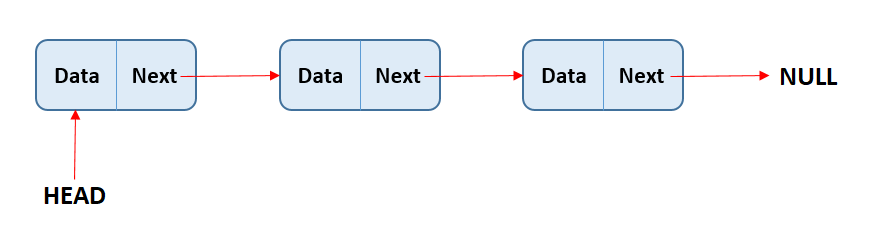
\includegraphics[width=0.8\textwidth]{aulas/aula3-lista-ligada1.png}
    \caption{Um nó}
  \end{figure}
\end{frame}

% Slide: Definição de Nó em C (Struct)
\begin{frame}[fragile]
  \frametitle{Definição de Nó em C (Struct)}
  \begin{lstlisting}[language=C]
typedef struct Node {
    int data; // Dados armazenados no nó
    struct Node* next; // Ponteiro para o próximo nó
} Node;
  \end{lstlisting}
  \begin{itemize}
    \item Esta \texttt{struct} define um nó de uma lista ligada simples em C.
    \item \texttt{data} armazena o valor do nó.
    \item \texttt{next} é um ponteiro para o próximo nó na lista, permitindo a ligação entre os nós.
  \end{itemize}
\end{frame}

% Slide: Definição de Nó em JavaScript/TypeScript
\begin{frame}[fragile]
  \frametitle{Definição de Nó em JavaScript/TypeScript}
  \begin{lstlisting}[language=JavaScript]
class Node {
    constructor(public data: number, public next: Node | null = null) {}
}
  \end{lstlisting}
  \begin{itemize}
    \item Esta classe define um nó de uma lista ligada em JavaScript/TypeScript.
    \item \texttt{data} é a propriedade que armazena o valor do nó.
    \item \texttt{next} é uma propriedade que aponta para o próximo nó na lista, inicialmente nulo se não especificado.
    \item A sintaxe \texttt{public} no construtor automaticamente declara e inicializa as propriedades da classe.
  \end{itemize}
\end{frame}

% Tipos de Listas Ligadas
% Slide: Lista Ligada Simples
\begin{frame}[fragile]
  \frametitle{Lista Ligada Simples}
  \begin{itemize}
    \item \textbf{Definição:} Uma lista ligada simples consiste em nós onde cada nó tem um ponteiro que aponta para o próximo nó na sequência.
    \item \textbf{Terminação:} O último nó aponta para NULL, indicando o fim da lista.
    \item \textbf{Operações:} Suporta operações básicas como inserção, remoção e travessia de forma eficiente, principalmente quando se trabalha no início da lista.
    \item \textbf{Uso:} Ideal para implementações simples onde a travessia é majoritariamente feita em uma única direção.
  \end{itemize}
\end{frame}

\begin{frame}[fragile]
  \frametitle{Lista ligada}
  \begin{figure}
    \centering
    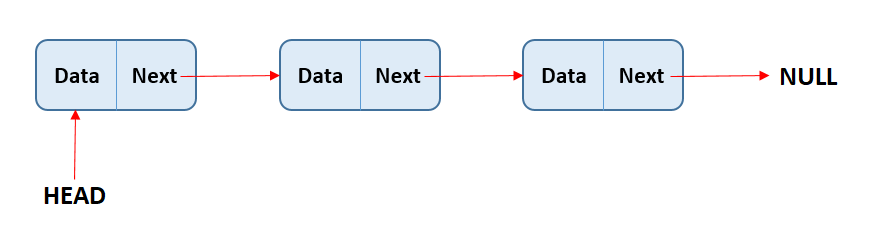
\includegraphics[width=0.8\textwidth]{aulas/aula3-lista-ligada1.png}
    \caption{Lista ligada}
  \end{figure}
\end{frame}
% Slide: Lista Duplamente Ligada
\begin{frame}[fragile]
  \frametitle{Lista Duplamente Ligada}
  \begin{itemize}
    \item \textbf{Definição:} Em uma lista duplamente ligada, cada nó contém dois ponteiros, um apontando para o próximo nó e outro para o anterior.
    \item \textbf{Flexibilidade:} Permite travessia nos dois sentidos (para frente e para trás), facilitando operações como reversão da lista e remoção de nós.
    \item \textbf{Uso de Memória:} Requer mais memória por nó em comparação com a lista ligada simples devido aos ponteiros extras.
    \item \textbf{Aplicações:} Útil em aplicações que necessitam de travessias bidirecionais ou inserções/remoções eficientes em qualquer ponto da lista.
  \end{itemize}
\end{frame}

\begin{frame}[fragile]
  \frametitle{Lista duplamente ligada}
  \begin{figure}
    \centering
    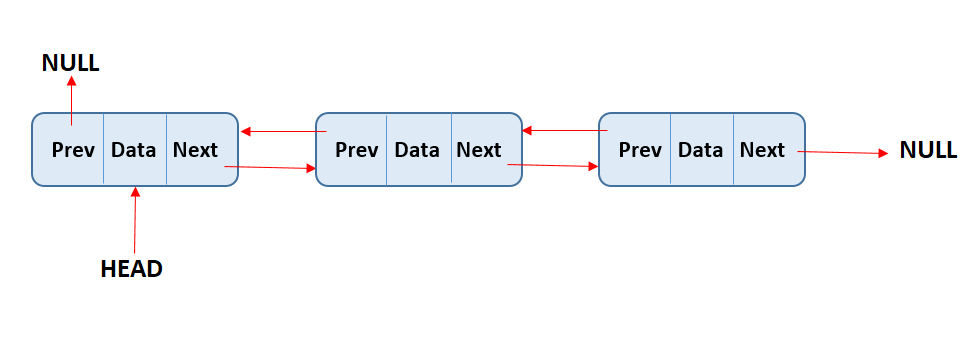
\includegraphics[width=0.8\textwidth]{aulas/aula3-dll.png}
    \caption{DLL}
  \end{figure}
\end{frame}
% Slide: Lista Circular
\begin{frame}[fragile]
  \frametitle{Lista Circular}
  \begin{itemize}
    \item \textbf{Definição:} Uma variação da lista ligada onde o último nó aponta de volta para o primeiro nó, formando um círculo.
    \item \textbf{Característica:} Não tem um fim claro como as listas ligadas simples ou duplamente ligadas, permitindo travessia contínua pela lista.
    \item \textbf{Considerações:} A implementação e a manutenção podem ser mais complexas, especialmente em listas circulares duplamente ligadas.
    \item \textbf{Uso:} Ideal para aplicações que necessitam de um ciclo contínuo de elementos, como algoritmos de round robin.
  \end{itemize}
\end{frame}

\begin{frame}[fragile]
  \frametitle{Lista circular}
  \begin{figure}
    \centering
    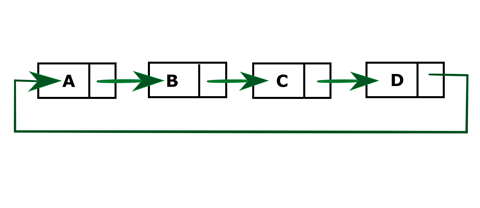
\includegraphics[width=0.8\textwidth]{aulas/aula3-cll.png}
    \caption{Lista circular}
  \end{figure}
\end{frame}

% Operações Básicas
\begin{frame}[fragile]
\frametitle{Operações Básicas}
\begin{itemize}
\item \textbf{Inserção:} Adiciona um novo nó à lista.
\begin{itemize}
\item No início, no meio, ou no fim da lista.
\end{itemize}
\item \textbf{Remoção:} Remove um nó da lista.
\begin{itemize}
\item Requer a atualização dos ponteiros do nó anterior e/ou posterior.
\end{itemize}
\item \textbf{Busca:} Encontra um nó na lista.
\begin{itemize}
\item Pode ser realizada iterando-se através dos nós até encontrar o desejado.
\end{itemize}
\item \textbf{Travessia:} Acessa cada nó da lista sequencialmente.
\end{itemize}
\end{frame}
% Slide: Inserção em Lista Ligada
\begin{frame}[fragile]
  \frametitle{Inserção em Lista Ligada}
  \begin{block}{Descrição}
    Adiciona um novo nó à lista. Pode ser realizado no início, no meio ou no fim da lista.
  \end{block}
  \small
  \begin{block}{Código em Portugol}
    procedimento inserirNoInicio(lista, valor) \\
    inicio \\
    \ \ novoNo := novo Nó \\
    \ \ novoNo.dado := valor \\
    \ \ novoNo.proximo := lista.cabeca \\
    \ \ lista.cabeca := novoNo \\
    fim
  \end{block}
\end{frame}

% Slide: Remoção em Lista Ligada
\begin{frame}[fragile]
  \frametitle{Remoção em Lista Ligada}
  \begin{block}{Descrição}
    Remove um nó da lista. Requer a atualização dos ponteiros do nó anterior (se houver) para apontar para o próximo nó do que está sendo removido.
  \end{block}
  
\end{frame}
\begin{frame}[fragile]
  \frametitle{Remoção em Lista Ligada - Código em Portugol}
  \small
  \begin{block}{Código em Portugol}
    procedimento removerNo(lista, valor) \\
    inicio \\
    \ \ se lista.cabeca = nulo então retorne fimSe \\
    \ \ se lista.cabeca.dado = valor então \\
    \ \ \ \ lista.cabeca := lista.cabeca.proximo \\
    \ \ senao \\
    \ \ \ \ atual := lista.cabeca \\
    \ \ \ \ enquanto atual.proximo ≠ nulo e atual.proximo.dado ≠ valor faça \\
    \ \ \ \ \ \ atual := atual.proximo \\
    \ \ \ \ fimEnquanto \\
    \ \ \ \ se atual.proximo ≠ nulo então \\
    \ \ \ \ \ \ atual.proximo := atual.proximo.proximo \\
    \ \ \ \ fimSe \\
    \ \ fimSe \\
    fim
  \end{block}
\end{frame}

% Slide: Busca em Lista Ligada
\begin{frame}[fragile]
  \frametitle{Busca em Lista Ligada}
  \begin{block}{Descrição}
    Encontra um nó na lista. A busca é realizada iterando-se através dos nós até encontrar o desejado.
  \end{block}
  \small
  \begin{block}{Código em Portugol}
    funcao buscarNo(lista, valor) : Nó \\
    inicio \\
    \ \ atual := lista.cabeca \\
    \ \ enquanto atual ≠ nulo faça \\
    \ \ \ \ se atual.dado = valor então \\
    \ \ \ \ \ \ retorne atual \\
    \ \ \ \ fimSe \\
    \ \ \ \ atual := atual.proximo \\
    \ \ fimEnquanto \\
    \ \ retorne nulo \\
    fim
  \end{block}
\end{frame}

% Slide: Travessia em Lista Ligada
\begin{frame}[fragile]
  \frametitle{Travessia em Lista Ligada}
  \begin{block}{Descrição}
    Acessa cada nó da lista sequencialmente. Utilizado para imprimir todos os elementos, ou para aplicar uma função a cada elemento da lista.
  \end{block}
  \small
  \begin{block}{Código em Portugol}
    procedimento percorrerLista(lista) \\
    inicio \\
    \ \ atual := lista.cabeca \\
    \ \ enquanto atual ≠ nulo faça \\
    \ \ \ \ escreva(atual.dado) \\
    \ \ \ \ atual := atual.proximo \\
    \ \ fimEnquanto \\
    fim
  \end{block}
\end{frame}

% Vantagens e Desvantagens
\begin{frame}[fragile]
\frametitle{Vantagens e Desvantagens}
\begin{itemize}
\item \textbf{Vantagens:}
\begin{itemize}
\item Flexibilidade no tamanho.
\item Inserção e remoção eficientes.
\end{itemize}
\item \textbf{Desvantagens:}
\begin{itemize}
\item Acesso sequencial (não aleatório) aos elementos.
\item Maior uso de memória devido aos ponteiros.
\end{itemize}
\end{itemize}
\end{frame}


% \title{Introdução a Filas e Pilhas}
\date{\today}
\frame{\titlepage}
% Slide 1: Conceito Detalhado de Filas
\begin{frame}[fragile]
  \frametitle{Conceito Detalhado de Filas}
  \begin{itemize}
    \item \textbf{Definição:} Uma fila é uma estrutura de dados linear que segue uma ordem específica para operações de adição e remoção de elementos. Essa ordem é baseada no princípio FIFO (First In, First Out), onde o primeiro elemento adicionado é o primeiro a ser removido.
    \item \textbf{Representação:} Visualmente, pode-se imaginar uma fila como uma linha de pessoas esperando para ser atendida em um banco, onde a primeira pessoa a chegar é a primeira a ser atendida.
    \item \textbf{Utilização:} Fundamental em situações que exigem manutenção da ordem original de eventos ou dados, como em sistemas operacionais para gerenciamento de processos e tarefas.
  \end{itemize}
\end{frame}

% Slide 2: Operações e Implementação de Filas
\begin{frame}[fragile]
  \frametitle{Operações e Implementação de Filas}
  \begin{itemize}
    \item \textbf{Operações Principais:}
      \begin{itemize}
        \item \textit{Enqueue (Inserir):} Adiciona um elemento ao final da fila.
        \item \textit{Dequeue (Remover):} Remove e retorna o elemento no início da fila.
        \item \textit{Peek/Front:} Retorna o elemento no início da fila sem removê-lo.
      \end{itemize}
    \item \textbf{Implementação:} Filas podem ser implementadas usando arrays ou listas ligadas. A escolha depende das necessidades específicas de desempenho e memória da aplicação.
  \end{itemize}
\end{frame}

% Slide 2: Operações e Implementação de Filas
\begin{frame}[fragile]
  \frametitle{Operações e Implementação de Filas}
  \begin{itemize}
    
    \item \textbf{Exemplo em Pseudocódigo:}
      \begin{verbatim}
      Enqueue(x):
        fila.append(x)
      
      Dequeue():
        if fila não está vazia:
          return fila.pop(0)
        else:
          return "Fila vazia"
      \end{verbatim}
  \end{itemize}
\end{frame}


% Slide: O Princípio FIFO e sua Aplicação em Filas
\begin{frame}[fragile]
  \frametitle{O Princípio FIFO e sua Aplicação em Filas}
  \begin{itemize}
    \item \textbf{Entendendo FIFO:} FIFO, sigla para First In, First Out, é um princípio fundamental de organização e processamento que estipula que o primeiro elemento a ser adicionado à estrutura será o primeiro a ser removido. Este conceito é essencial em muitas estruturas de dados, com destaque para as filas.
    \item \textbf{Importância em Filas:}
      \begin{itemize}
        \item Garante justiça e ordem na execução de tarefas ou no atendimento de solicitações, assegurando que não haja favorecimento ou atrasos indevidos.
        \item Facilita o planejamento e a previsão em sistemas de processamento, permitindo estimar o tempo de espera e alocar recursos de forma eficiente.
      \end{itemize}
  \end{itemize}
\end{frame}
\begin{frame}[fragile]
  \frametitle{O Princípio FIFO e sua Aplicação em Filas}
  \begin{itemize}
    \item \textbf{Aplicações Práticas:}
      \begin{itemize}
        \item \textit{Sistemas de Atendimento:} Em um restaurante com sistema de fila de espera, o cliente que chega primeiro, é atendido primeiro.
        \item \textit{Processamento de Tarefas:} Em um sistema operacional, processos em uma fila de execução são iniciados com base na sua ordem de chegada, garantindo um tratamento equitativo dos recursos do sistema.
      \end{itemize}
    \item \textbf{Conclusão:} O princípio FIFO é a espinha dorsal das filas, proporcionando uma base sólida para o desenvolvimento de algoritmos justos e eficientes em diversas áreas da computação e do cotidiano.
  \end{itemize}
\end{frame}


% Slide 3: Aplicação Prática de Filas
\begin{frame}[fragile]
  \frametitle{Aplicação Prática de Filas}
  \begin{itemize}
    \item \textbf{Gerenciamento de Tarefas em Sistemas Operacionais:} Um exemplo prático do uso de filas é no escalonamento de processos em sistemas operacionais. Processos são mantidos em uma fila, aguardando pela CPU. O agendador de tarefas seleciona processos da fila seguindo a ordem FIFO para execução.
    \item \textbf{Simulação de Cenário:}
      \begin{itemize}
        \item \textit{Situação:} Uma fila de impressão onde documentos são adicionados e impressos seguindo a ordem de chegada.
        \item \textit{Implementação:} A aplicação da fila garante que todos os documentos serão impressos na ordem correta, evitando conflitos e garantindo a equidade no uso da impressora.
      \end{itemize}
    \item \textbf{Benefício:} O uso de filas em tais sistemas assegura a transparência e eficiência no processamento de tarefas ou atendimento de solicitações.
  \end{itemize}
\end{frame}
% Slide: Aplicação de Filas em Sistemas de Gerenciamento de Filas
\begin{frame}[fragile]
  \frametitle{Aplicação de Filas em Sistemas de Gerenciamento de Filas}
  \begin{itemize}
    \item \textbf{Contexto:} Bancos, supermercados e repartições públicas onde o serviço é prestado com base na ordem de chegada dos clientes.
    \item \textbf{Implementação:} Utiliza-se uma fila para organizar os clientes de acordo com sua chegada, garantindo que o atendimento seja feito de forma justa e eficiente.
    \item \textbf{Benefícios:}
      \begin{itemize}
        \item Garantia de atendimento por ordem de chegada.
        \item Redução de conflitos e insatisfação dos clientes.
        \item Melhoria na previsibilidade e gestão do tempo de espera.
      \end{itemize}
    \item \textbf{Exemplo Prático:} Um sistema de senha em um banco, onde cada cliente retira uma senha ao entrar e é atendido quando seu número é chamado, seguindo estritamente a ordem de chegada.
  \end{itemize}
\end{frame}

% Slide: Aplicação de Filas no Processamento de Dados
\begin{frame}[fragile]
  \frametitle{Aplicação de Filas no Processamento de Dados}
  \begin{itemize}
    \item \textbf{Contexto:} Processamento e armazenamento temporário de dados em sistemas computacionais, como em streams de vídeo ou impressão de documentos.
    \item \textbf{Implementação:} Dados são colocados em uma fila, onde o primeiro a chegar será o primeiro a ser processado ou transmitido, garantindo a ordem correta de processamento.
    \item \textbf{Benefícios:}
      \begin{itemize}
        \item Mantém a integridade e a sequência dos dados durante o processamento.
        \item Facilita o gerenciamento de carga em sistemas de processamento, evitando sobrecarga e otimizando o uso dos recursos.
      \end{itemize}
    \item \textbf{Exemplo Prático:} Uma fila de impressão onde documentos enviados para a impressora são armazenados em uma fila e impressos na ordem em que foram recebidos.
  \end{itemize}
\end{frame}

% Slide: Aplicação de Filas no Controle de Tráfego de Redes
\begin{frame}[fragile]
  \frametitle{Aplicação de Filas no Controle de Tráfego de Redes}
  \begin{itemize}
    \item \textbf{Contexto:} Gerenciamento do fluxo de dados em redes de computadores, como na Internet ou em redes corporativas.
    \item \textbf{Implementação:} Filas são usadas para controlar o envio de pacotes de dados, garantindo que sejam enviados e recebidos em uma ordem lógica e eficiente.
    \item \textbf{Benefícios:}
      \begin{itemize}
        \item Priorização do tráfego, permitindo que pacotes críticos sejam processados antes.
        \item Prevenção de congestionamento na rede, gerenciando eficientemente o volume de dados.
      \end{itemize}
    \item \textbf{Exemplo Prático:} Em roteadores e switches, filas são utilizadas para ordenar pacotes de dados quando há mais dados chegando do que a capacidade de processamento ou largura de banda disponível, evitando a perda de dados importantes.
  \end{itemize}
\end{frame}

\end{frame}

% Slide 3: Introdução a Pilhas
% Slide: Conceito Detalhado de Pilhas
\begin{frame}[fragile]
  \frametitle{Conceito Detalhado de Pilhas}
  \begin{itemize}
    \item \textbf{Definição:} Pilhas são estruturas de dados abstratas que operam sob o princípio LIFO (Last In, First Out), onde o último elemento adicionado é o primeiro a ser removido.
    \item \textbf{Analogia Visual:} Imagine uma pilha de pratos em uma bandeja. O último prato colocado no topo é o primeiro a ser retirado quando necessário.
    \item \textbf{Características:}
      \begin{itemize}
        \item Simplicidade na adição e remoção de elementos, pois ocorrem no mesmo ponto.
        \item Facilidade na implementação em diversas linguagens de programação.
        \item Eficiência no gerenciamento de dados temporários, como históricos de navegação ou chamadas de funções.
      \end{itemize}
  \end{itemize}
\end{frame}

% Slide: Aplicações Práticas de Pilhas
\begin{frame}[fragile]
  \frametitle{Aplicações Práticas de Pilhas}
  \begin{itemize}
    \item \textbf{Execução de Chamadas de Função:} Pilhas são essenciais para gerenciar chamadas de função em programas, armazenando endereços de retorno e variáveis locais.
    \item \textbf{Avaliação de Expressões:} Utilizadas para avaliar expressões aritméticas e lógicas em notações como a postfix (polonesa inversa), facilitando a computação.
    \item \textbf{Navegação e Histórico:} Em interfaces de usuário, como navegadores web, pilhas ajudam a gerenciar o histórico de páginas visitadas, permitindo ao usuário retornar às páginas anteriores.
    \item \textbf{Desfazer Ações em Aplicativos:} Muitos softwares utilizam pilhas para permitir que os usuários desfaçam (undo) ações recentes de maneira ordenada e eficiente.
  \end{itemize}
\end{frame}

% Slide: Operações Básicas em Pilhas
\begin{frame}[fragile]
  \frametitle{Operações Básicas em Pilhas}
  \begin{itemize}
    \item \textbf{Push (Inserir):} Adiciona um elemento ao topo da pilha. É a operação que aumenta o tamanho da pilha, inserindo um novo elemento como o mais recente.
    \item \textbf{Pop (Remover):} Remove e retorna o elemento do topo da pilha. Esta operação diminui o tamanho da pilha, removendo o elemento que foi adicionado por último.
    \item \textbf{Peek/Top (Observar):} Retorna o elemento no topo da pilha sem removê-lo. Essencial para verificar o estado atual da pilha sem alterá-la.
  \end{itemize}
\end{frame}

\begin{frame}[fragile]
  \frametitle{Operações Básicas em Pilhas}
  \begin{itemize}
    \item \textbf{Exemplo em Pseudocódigo:}
    \small
    \begin{verbatim}
      push(x):
        pilha.add(x)

      pop():
        if pilha não está vazia:
          return pilha.remove(topo)
        else:
          return "Pilha vazia"

      peek():
        if pilha não está vazia:
          return pilha[topo]
        else:
          return "Pilha vazia"
      \end{verbatim}
  \end{itemize}
\end{frame}


% Slide 4: Exemplo de Aplicação de Pilhas
% Slide: Aplicação de Pilhas em Navegação na Web
\begin{frame}[fragile]
  \frametitle{Aplicação de Pilhas em Navegação na Web}
  \begin{itemize}
    \item \textbf{Contexto:} A navegação em sites na internet, onde cada página visitada é armazenada sequencialmente.
    \item \textbf{Implementação:} Uma pilha é usada para armazenar o histórico de páginas visitadas. Ao visitar uma nova página, a URL é "empilhada" no topo. Quando o usuário clica no botão de voltar, a página no topo da pilha é "desempilhada", e o navegador retorna à página anterior.
    \item \textbf{Vantagens:}
      \begin{itemize}
        \item Permite uma navegação intuitiva e eficiente entre as páginas visitadas.
        \item Facilita a implementação de recursos de histórico em navegadores web.
      \end{itemize}
    \item \textbf{Exemplo Prático:} Ao explorar links em uma página de notícias e depois utilizar o botão de voltar, o navegador usa uma pilha para determinar qual foi a última página visitada.
  \end{itemize}
\end{frame}

% Slide: Pilhas na Execução de Chamadas de Função
\begin{frame}[fragile]
  \frametitle{Pilhas na Execução de Chamadas de Função}
  \begin{itemize}
    \item \textbf{Contexto:} Programação de software, onde funções chamam outras funções durante a execução.
    \item \textbf{Implementação:} Cada chamada de função cria um novo quadro de pilha (stack frame) no topo da pilha, contendo informações como o ponto de retorno e variáveis locais. Quando uma função retorna, seu quadro de pilha é removido, retornando ao ponto de chamada.
    \item \textbf{Vantagens:}
      \begin{itemize}
        \item Garante a correta execução de funções e o retorno aos pontos de chamada apropriados.
        \item Facilita o rastreamento de chamadas de função e a depuração de programas.
      \end{itemize}
    \item \textbf{Exemplo Prático:} Em um programa que calcula fatorial, a função de fatorial chama a si mesma para cada valor decrementado até que atinja a base da recursão, utilizando uma pilha para controlar cada chamada.
  \end{itemize}
\end{frame}

% Slide: Pilhas na Avaliação de Expressões
\begin{frame}[fragile]
  \frametitle{Pilhas na Avaliação de Expressões}
  \begin{itemize}
    \item \textbf{Contexto:} Avaliação de expressões matemáticas, especialmente a conversão e avaliação de expressões infixas para postfixas (notação polonesa reversa).
    \item \textbf{Implementação:} Pilhas são usadas para armazenar operadores e operandos durante a conversão de expressões infixas para postfixas e durante a avaliação de expressões postfixas.
    \item \textbf{Vantagens:}
      \begin{itemize}
        \item Simplifica a computação ao eliminar a necessidade de considerar precedências de operadores fora da ordem.
        \item Torna mais eficiente a avaliação de expressões complexas em calculadoras e interpretadores de linguagem.
      \end{itemize}
    \item \textbf{Exemplo Prático:} Uma calculadora que avalia a expressão "3 + 4 * 2" primeiro converte para a forma postfixa "3 4 2 * +", depois avalia usando uma pilha para armazenar temporariamente os operandos e resultados parciais.
  \end{itemize}
\end{frame}
\begin{frame}[fragile]
  \frametitle{Jogo Torre de Hanoi}
  \begin{figure}
    \centering
    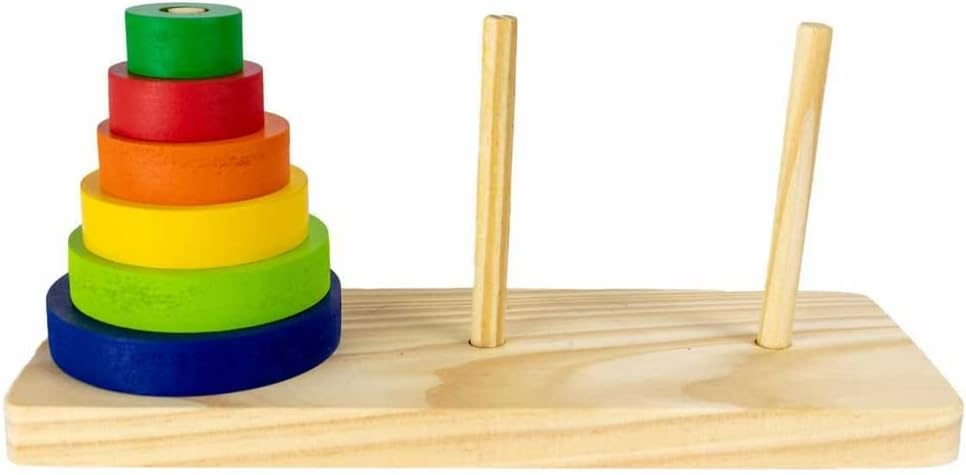
\includegraphics[width=0.8\textwidth]{assets/aula4-hanoi.jpg}
    \caption{Torre de Hanoi}
  \end{figure}
\end{frame}
% Slide: Introdução ao Problema da Torre de Hanoi
\begin{frame}[fragile]
  \frametitle{Introdução ao Problema da Torre de Hanoi}
  \begin{itemize}
    \item \textbf{Descrição do Problema:} O jogo da Torre de Hanoi consiste em três hastes e um número de discos de diferentes tamanhos que podem ser encaixados em qualquer haste. O objetivo é mover todos os discos de uma haste para outra, seguindo três regras simples:
      \begin{enumerate}
        \item Apenas um disco pode ser movido de cada vez.
        \item Cada movimento consiste em pegar o disco superior de uma das pilhas e colocá-lo no topo de outra pilha.
        \item Um disco maior não pode ser colocado sobre um disco menor.
      \end{enumerate}
    \item \textbf{Objetivo:} Mover todos os discos da haste origem para a haste destino, utilizando a haste auxiliar conforme necessário, com o menor número de movimentos possíveis.
  \end{itemize}
\end{frame}

% Slide: Algoritmo da Torre de Hanoi
\begin{frame}[fragile]
  \frametitle{Algoritmo da Torre de Hanoi}
  \begin{itemize}
    \item \textbf{Descrição do Algoritmo:} O algoritmo para resolver a Torre de Hanoi é um belo exemplo de aplicação de recursão. O processo pode ser descrito da seguinte forma:
      \begin{enumerate}
        \item Mover \(n - 1\) discos da haste origem para a haste auxiliar, usando a haste destino como intermediária.
        \item Mover o disco restante (o maior) para a haste destino.
        \item Mover os \(n - 1\) discos da haste auxiliar para a haste destino, usando a haste origem como intermediária.
      \end{enumerate}
    \item \textbf{Base da Recursão:} Quando resta apenas um disco, esse disco pode ser movido diretamente para a haste destino.
  \end{itemize}
\end{frame}

% Slide: Exemplo Prático do Algoritmo da Torre de Hanoi
\begin{frame}[fragile]
  \frametitle{Exemplo Prático do Algoritmo da Torre de Hanoi}
  \begin{itemize}
    \item \textbf{Cenário:} Considere um jogo da Torre de Hanoi com 3 discos na haste A (origem), com as hastes B (auxiliar) e C (destino) vazias.
    \item \textbf{Passos para Solução:}
      \begin{enumerate}
        \item Mova os dois primeiros discos para a haste B, usando C como intermediária.
        \item Mova o disco maior (o terceiro) para a haste C.
        \item Mova os dois discos de B para C, usando A como intermediária.
      \end{enumerate}
    \item \textbf{Resultado:} Todos os discos estão agora na haste C, na mesma ordem original, mas na haste destino, completando o jogo.
    \item \textbf{Nota:} Este procedimento minimiza o número total de movimentos necessários para resolver o jogo para qualquer número de discos.
  \end{itemize}
\end{frame}

\begin{frame}[fragile]
  \frametitle{Validação de Strings com Parênteses, Chaves e Colchetes}

  \textbf{Problema:} Dada uma string \(s\) contendo apenas os caracteres '(', ')', '{', '}', '[' e ']', determinar se a string de entrada é válida.

  \textbf{Critérios para uma string válida:}
  \begin{itemize}
    \item Parênteses abertos devem ser fechados pelo mesmo tipo de parênteses.
    \item Parênteses abertos devem ser fechados na ordem correta.
    \item Todo parêntese de fechamento tem um correspondente parêntese de abertura do mesmo tipo.
  \end{itemize}

  \tiny 
  referência: https://leetcode.com/problems/valid-parentheses/description/
\end{frame}

\begin{frame}[fragile]
  \frametitle{Validação de Strings com Parênteses, Chaves e Colchetes}

  \textbf{Exemplos:}
  \begin{itemize}
    \item Entrada: \(s = "()"\) \\
          Saída: verdadeiro
    \item Entrada: \(s = "()[]{}"\) \\
          Saída: verdadeiro
    \item Entrada: \(s = "(]"\) \\
          Saída: falso
  \end{itemize}

  \textbf{Restrições:}
  \begin{itemize}
    \item \(1 \leq \text{comprimento de } s \leq 10^4\)
    \item \(s\) consiste apenas de parênteses '()[]{}'.
  \end{itemize}
  \tiny 
  referência: https://leetcode.com/problems/valid-parentheses/description/
\end{frame}


\begin{frame}[fragile]
  \frametitle{Introdução à Notação Polonesa}
  
  \textbf{O que é Notação Polonesa (Notação Polonesa Reversa)?}
  \begin{itemize}
    \item Método de notação matemática onde cada operador segue todos os seus operandos.
    \item Remove a necessidade de parênteses para indicar a ordem das operações.
    \item Exemplo: A expressão convencional "3 + 4" é expressa como "3 4 +" na notação polonesa reversa.
  \end{itemize}
  
  \textbf{Vantagens da Notação Polonesa:}
  \begin{itemize}
    \item Simplifica a leitura e avaliação de expressões matemáticas.
    \item Elimina ambiguidades na ordem das operações sem o uso de parênteses.
  \end{itemize}
\end{frame}
\begin{frame}[fragile]
  \frametitle{Vantagens da Notação Polonesa Reversa}
  
  \textbf{Por que usar Notação Polonesa Reversa?}
  \begin{itemize}
    \item \textbf{Simplicidade de Avaliação:} Permite avaliação de expressões de forma sequencial, da esquerda para a direita.
    \item \textbf{Não Requer Parênteses:} A ordem de execução das operações é claramente definida pela posição dos operadores e operandos.
  \end{itemize}
  
  \textbf{Aplicações Práticas:}
  \begin{itemize}
    \item Amplamente utilizada em calculadoras científicas e em alguns tipos de computação.
    \item Facilita a implementação de algoritmos de avaliação de expressões em linguagens de programação.
  \end{itemize}
\end{frame}
\begin{frame}[fragile]
  \frametitle{A Importância das Pilhas na Notação Polonesa}
  
  \textbf{Como as Pilhas Facilitam a Avaliação:}
  \begin{itemize}
    \item Pilhas armazenam temporariamente os operandos durante a avaliação de expressões.
    \item Operadores aplicam-se aos elementos no topo da pilha; o resultado é recolocado na pilha.
  \end{itemize}
  
  \textbf{Benefícios do Uso de Pilhas:}
  \begin{itemize}
    \item Permite processamento direto e eficiente de expressões complexas.
    \item Essencial para a implementação de algoritmos de avaliação de expressões matemáticas em notação polonesa reversa.
  \end{itemize}
  
  \textbf{Conclusão:}
  O uso de pilhas é fundamental na notação polonesa reversa, oferecendo uma abordagem eficiente para o processamento de operações matemáticas.
\end{frame}
\begin{frame}[fragile]
  \frametitle{Exemplo de Cálculo em Notação Polonesa Reversa}

  \textbf{Expressão:} \(3\ 4\ +\ 2\ \ast\)

  \textbf{Objetivo:} Calcular a expressão usando notação polonesa reversa.
  
  \textbf{Processo:}

  \begin{enumerate}
    \item Iniciar com uma pilha vazia.
    \item Ler os elementos da expressão da esquerda para a direita:
      \begin{enumerate}
        \item Empilhar \(3\).
        \item Empilhar \(4\).
        \item Ler '+': desempilhar dois últimos números (\(4\) e \(3\)), somá-los (\(7\)), e empilhar o resultado (\(7\)).
        \item Empilhar \(2\).
        \item Ler '\(\ast\)': desempilhar dois últimos números (\(2\) e \(7\)), multiplicá-los (\(14\)), e empilhar o resultado (\(14\)).
      \end{enumerate}
    \item O resultado final (\(14\)) está no topo da pilha.
  \end{enumerate}

  \textbf{Resultado:} A expressão \(3\ 4\ +\ 2\ \ast\) é avaliada como \(14\), equivalente a \((3 + 4) \ast 2\) na notação convencional.
\end{frame}
\begin{frame}[fragile]
  \frametitle{Exemplo Complexo de Cálculo em Notação Polonesa Reversa}

  \textbf{Entrada:} tokens = ["10", "6", "9", "3", "+", "-11", "*", "/", "*", "17", "+", "5", "+"]

  \textbf{Objetivo:} Calcular a expressão usando notação polonesa reversa para obter o resultado 22.

  
\end{frame}

\begin{frame}[fragile]
  \frametitle{Exemplo Complexo de Cálculo em Notação Polonesa Reversa}



  \begin{enumerate}
    \item Expressão original em notação convencional: \(((10 \ast (6 / ((9 + 3) \ast -11))) + 17) + 5\)
    \item Simplificação passo a passo:
      \begin{enumerate}
        \item \(9 + 3 = 12\)
        \item \(12 \ast -11 = -132\)
        \item \(6 / -132 = 0\) (considerando divisão inteira)
        \item \(10 \ast 0 = 0\)
        \item \(0 + 17 = 17\)
        \item \(17 + 5 = 22\)
      \end{enumerate}
  \end{enumerate}

\end{frame}

\begin{frame}[fragile]
  \frametitle{Exemplo Complexo de Cálculo em Notação Polonesa Reversa}


  \begin{enumerate}
   
    \item Usando pilhas na notação polonesa reversa:
      \begin{enumerate}
        \item Empilha \(10, 6, 9, 3\), realiza \(9 + 3\) e empilha o resultado.
        \item Empilha \(-11\), realiza \(12 \ast -11\) e empilha o resultado.
        \item Realiza \(6 / -132\) (resultando em \(0\) com divisão inteira) e empilha.
        \item Empilha \(10\) e realiza \(10 \ast 0\), empilha o resultado.
        \item Empilha \(17\), realiza a adição com \(0\), e então empilha \(5\) e realiza a adição final.
      \end{enumerate}
    \item O resultado final no topo da pilha é \(22\).
  \end{enumerate}

  \textbf{Resultado:} A expressão complexa é avaliada como \(22\), demonstrando a eficácia da notação polonesa reversa e do uso de pilhas para avaliação de expressões matemáticas.
\end{frame}

% \title{Introdução a Árvores (Estruturas de Dados)}
\date{\today}
\frame{\titlepage}

% Slide 1: Introdução às Árvores como Conceito
\begin{frame}[fragile]
  \frametitle{Introdução às Árvores como Conceito}
  \begin{itemize}
    \item \textbf{Definição:} Uma árvore, em ciência da computação, é uma estrutura de dados hierárquica que simula uma estrutura de árvore com um conjunto de nós conectados.
    \item \textbf{Raízes Biológicas:} Inspirado nas árvores da natureza, onde um tronco se ramifica em muitos galhos, que por sua vez podem se dividir em mais galhos, até chegar às folhas.
    \item \textbf{Aplicabilidade:} Árvores são essenciais para representar estruturas organizacionais, árvores genealógicas e em várias estruturas de dados como árvores binárias, árvores AVL, árvores de segmento, etc.
  \end{itemize}
\end{frame}

% Slide 2: Estruturas Organizacionais e Árvores Genealógicas
\begin{frame}[fragile]
  \frametitle{Estruturas Organizacionais e Árvores Genealógicas}
  \begin{itemize}
    \item \textbf{Estruturas Organizacionais:} Utilizam o conceito de árvores para representar hierarquias dentro de uma organização, desde o nível mais alto de gestão até os funcionários de nível base.
    \item \textbf{Árvores Genealógicas:} Mostram as relações de parentesco entre os membros de uma família ao longo de gerações, onde cada pessoa pode ser vista como um nó conectado aos seus ascendentes e descendentes.
    \item \textbf{Visualização:} Ambos os exemplos ajudam a entender a utilidade das árvores na organização e na representação de relações hierárquicas complexas.
  \end{itemize}
\end{frame}
\begin{frame}[fragile]
  \frametitle{Estruturas Organizacionais}
  \begin{figure}
    \centering
    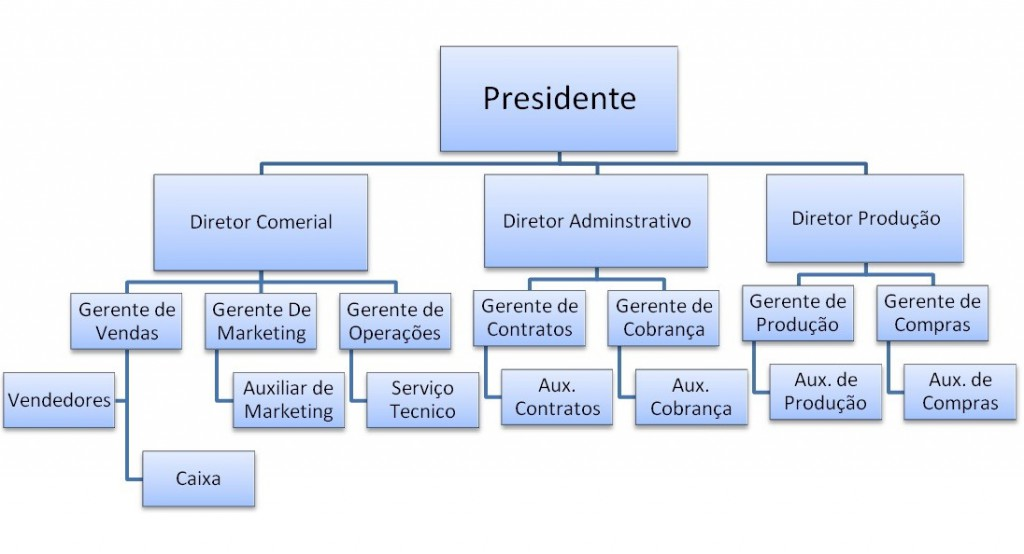
\includegraphics[width=0.7\textwidth]{assets/aula5-arvore-organograma.jpeg}
    \caption{Estruturas Organizacionais}
  \end{figure}
\end{frame}
\begin{frame}[fragile]
  \frametitle{Árvores Genealógicas}
  \begin{figure}
    \centering
    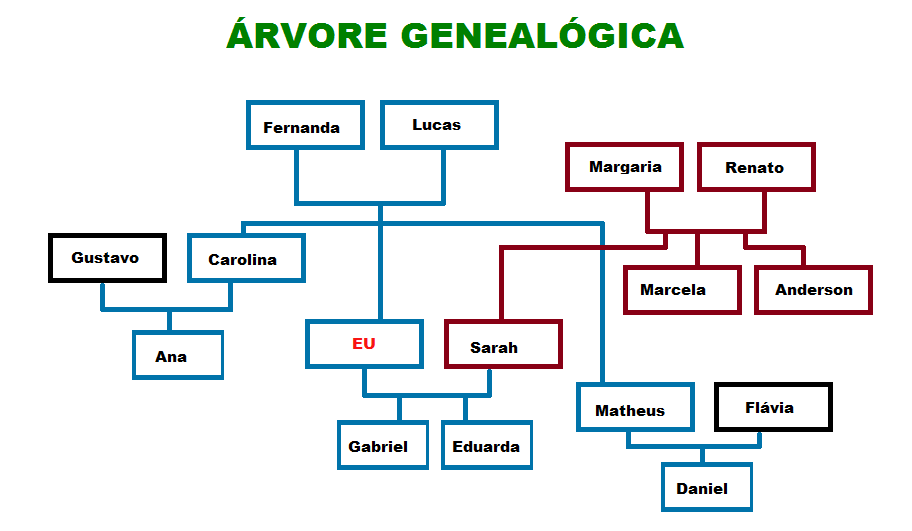
\includegraphics[width=0.7\textwidth]{assets/aula5-arvore-genealogica.png}
    \caption{Árvores Genealógicas}
  \end{figure}
\end{frame}
% Slide: Árvores de Decisão no Jogo da Velha
\begin{frame}[fragile]
  \frametitle{Árvores de Decisão no Jogo da Velha}
  \begin{itemize}
    \item \textbf{Conceito:} Uma árvore de decisão é um diagrama que representa decisões e seus possíveis resultados. No contexto de jogos, é usada para modelar as possibilidades de jogadas e seus desfechos.
    \item \textbf{Aplicação no Jogo da Velha:}
      \begin{itemize}
        \item Cada nó representa o estado atual do tabuleiro.
        \item Cada ramificação a partir de um nó representa uma jogada possível.
        \item Folhas da árvore representam o desfecho da partida (vitória, derrota ou empate).
      \end{itemize}
    \item \textbf{Utilização:} Árvores de decisão permitem a um algoritmo de IA antecipar movimentos, escolhendo o caminho que maximiza a chance de vitória ou minimiza a de derrota.
    \item \textbf{Desenvolvimento de Estratégias:} Analisando a árvore de decisão completa do jogo da velha, é possível desenvolver uma estratégia perfeita, onde a IA nunca perde, podendo no máximo empatar.
    \item \textbf{Implicações:} Este modelo é um exemplo fundamental de como técnicas simples de IA podem ser aplicadas para resolver problemas complexos em jogos e em outras áreas da computação.
  \end{itemize}
\end{frame}
\begin{frame}[fragile]
  \frametitle{Árvores de Decisão no Jogo da Velha}
  \begin{figure}
    \centering
    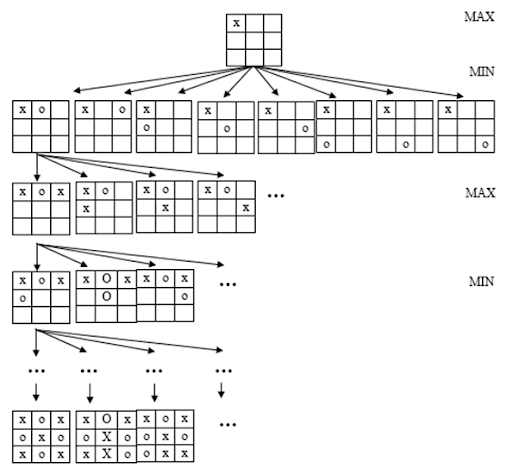
\includegraphics[width=0.7\textwidth]{assets/aula5-tic.png}
    \caption{Árvores de Decisão no Jogo da Velha}
  \end{figure}
\end{frame}


% Slide 3: Conceitos Básicos de Árvores em Estruturas de Dados
\begin{frame}[fragile]
  \frametitle{Conceitos Básicos de Árvores em Estruturas de Dados}
  \begin{itemize}
    \item \textbf{Nó:} Elemento básico que contém dados e links para outros nós (filhos).
    \item \textbf{Raiz:} Nó no topo da árvore, sem pais.
    \item \textbf{Folhas:} Nós sem filhos, localizados na base da árvore.
    \item \textbf{Altura:} Comprimento do caminho mais longo de um nó à uma folha.
  \end{itemize}
\end{frame}
\begin{frame}[fragile]
  \frametitle{Árvores em Estruturas de Dados}
  \begin{figure}
    \centering
    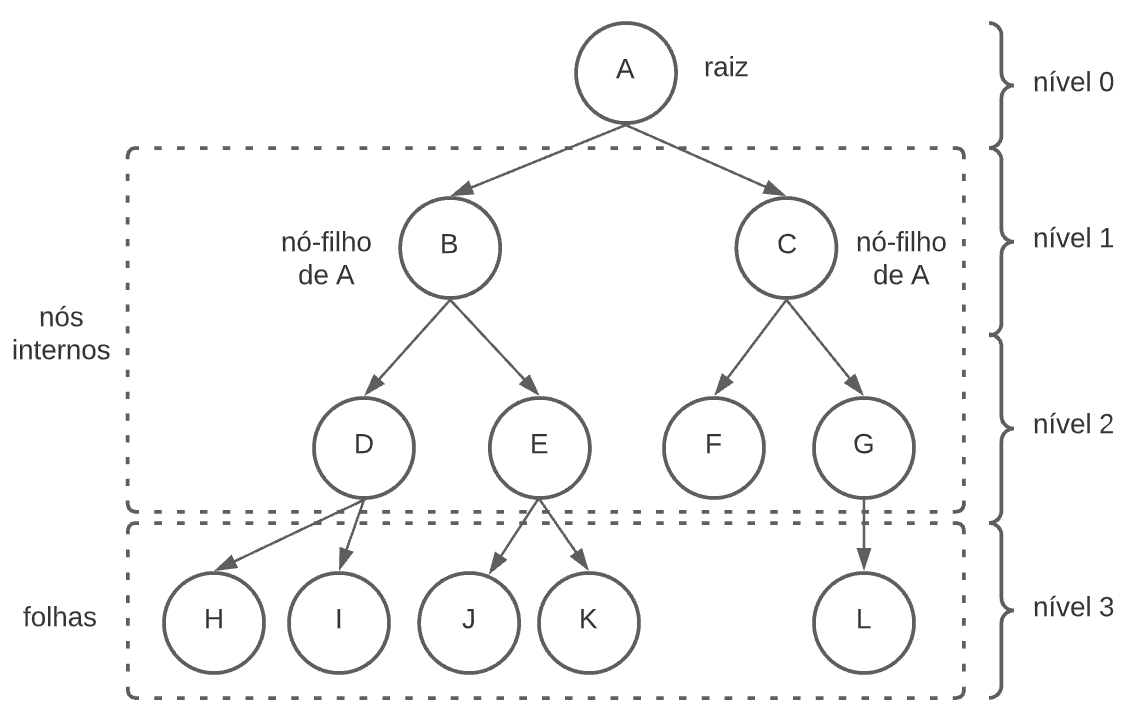
\includegraphics[width=0.7\textwidth]{assets/aula5-arvores1.png}
    \caption{Árvores em Estruturas de Dados}
  \end{figure}
\end{frame}

\begin{frame}[fragile]
  \frametitle{Inspecionando os elementos de uma árvore}
  \begin{figure}
    \centering
    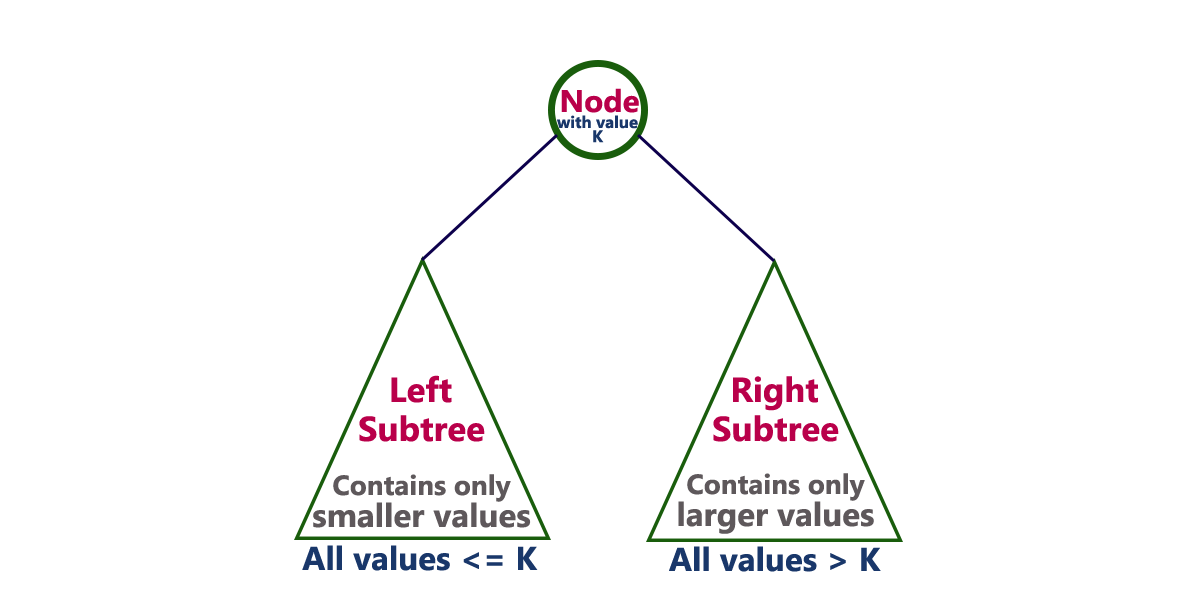
\includegraphics[width=0.5\textwidth]{assets/aula5-arvores3.png}
    \caption{Inspecionando os elementos de uma árvore}
  \end{figure}
\end{frame}
% Slide 4: Árvores Binárias e suas Operações
\begin{frame}[fragile]
  \frametitle{Árvores Binárias e suas Operações}
  \begin{itemize}
    \item \textbf{Definição:} Uma árvore binária é uma estrutura de árvore em que cada nó tem no máximo dois filhos, conhecidos como filho à esquerda e filho à direita.
    \item \textbf{Operações Principais:}
      \begin{itemize}
        \item \textit{Inserção:} Adiciona um novo nó na árvore na posição adequada.
        \item \textit{Remoção:} Remove um nó da árvore, mantendo as propriedades da árvore binária.
        \item \textit{Busca:} Encontra um valor dentro da árvore.
      \end{itemize}
    \item \textbf{Percursos:} Em ordem, pré-ordem e pós-ordem são métodos para visitar todos os nós de uma árvore binária.
  \end{itemize}
\end{frame}

% Slide 5: Aplicações Práticas de Árvores
\begin{frame}[fragile]
  \frametitle{Aplicações Práticas de Árvores}
  \begin{itemize}
    \item \textbf{Bancos de Dados:} Árvores B e árvores B+ são utilizadas em sistemas de gerenciamento de banco de dados para indexação e busca rápida de dados.
    \item \textbf{Gráficos de Computador:} Árvores são usadas em algoritmos de renderização para organizar e processar objetos em uma cena.
    \item \textbf{Redes:} Estruturas de árvore ajudam na organização e na otimização de redes, como em protocolos de roteamento.
    \item \textbf{Conclusão:} O estudo de árvores é fundamental na ciência da computação, com aplicações vastas e significativas em diversos campos.
  \end{itemize}
\end{frame}

\begin{frame}[fragile]
  \frametitle{Introdução às Árvores Binárias Não Balanceadas}
  \begin{itemize}
    \item \textbf{Definição:} Uma árvore binária não balanceada é uma estrutura de dados em que cada nó tem até dois filhos, mas sem garantias específicas sobre a altura da árvore, o que pode levar a desequilíbrios significativos no número de nós entre as subárvores esquerda e direita.
    \item \textbf{Propriedades:}
      \begin{itemize}
        \item Cada nó representa um elemento ou valor.
        \item Cada nó pode ter até dois filhos: um à esquerda e um à direita.
        \item Não há restrições específicas de balanceamento, permitindo que a árvore se torne assimétrica.
      \end{itemize}
    \item \textbf{Aplicabilidade:} Embora simples, as árvores binárias não balanceadas são fundamentais para entender conceitos mais avançados em estruturas de dados, como árvores balanceadas e árvores de busca.
  \end{itemize}
\end{frame}

\begin{frame}[fragile]
  \frametitle{Inspecionando os elementos de uma árvore}
  \begin{figure}
    \centering
    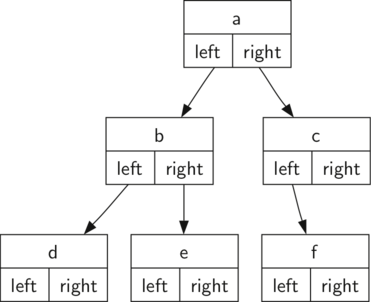
\includegraphics[width=0.5\textwidth]{assets/aula5-arvores2.png}
    \caption{Inspecionando os elementos de uma árvore}
  \end{figure}
\end{frame}
% Slide: Organização dos Nós
\begin{frame}[fragile]
  \frametitle{Organização dos Nós}
  \begin{itemize}
    \item \textbf{Regra Geral:}
      \begin{itemize}
        \item Nós à esquerda de um dado nó contêm valores menores.
        \item Nós à direita de um dado nó contêm valores maiores.
      \end{itemize}
    \item \textbf{Importância:} Esta organização facilita operações de busca, inserção e remoção, permitindo que operações como busca binária sejam realizadas eficientemente.
    \item \textbf{Exceções:} Em árvores binárias não necessariamente de busca, a organização dos nós pode seguir outras lógicas específicas, dependendo da aplicação.
  \end{itemize}
\end{frame}


\begin{frame}[fragile]
  \frametitle{Inspecionando os elementos de uma árvore}
  \begin{figure}
    \centering
    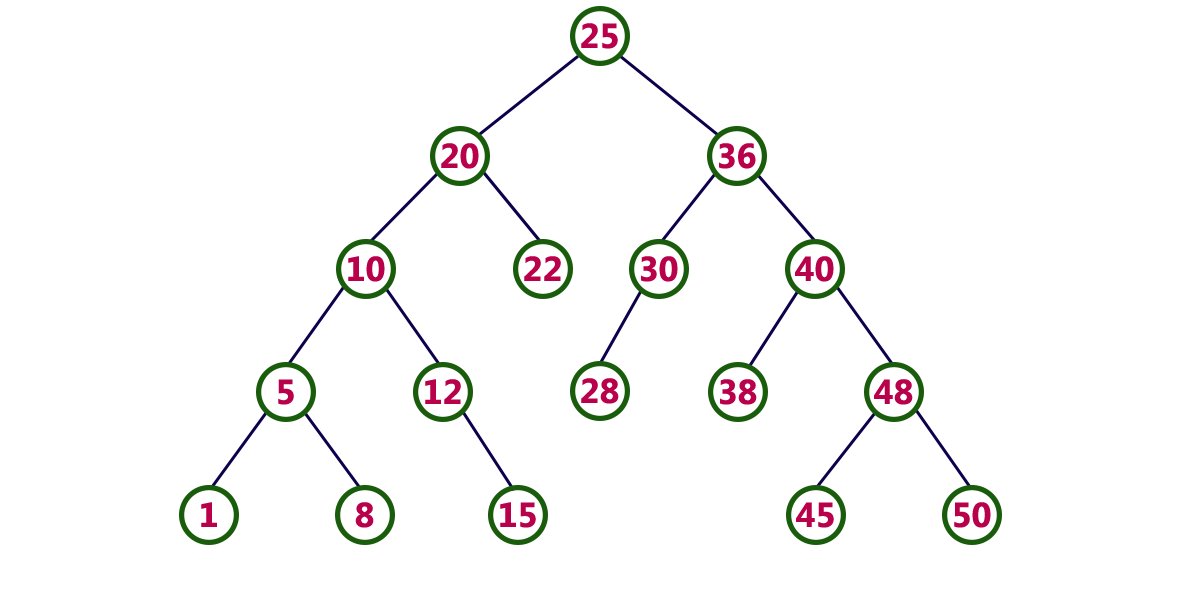
\includegraphics[width=0.5\textwidth]{assets/aula5-arvores4.png}
    \caption{Inspecionando os elementos de uma árvore}
  \end{figure}
\end{frame}
% Slide: Inserção em Árvores Binárias Não Balanceadas
\begin{frame}[fragile]
  \frametitle{Inserção em Árvores Binárias Não Balanceadas}
  \begin{itemize}
    \item \textbf{Processo de Inserção:}
      \begin{itemize}
        \item Iniciar no nó raiz.
        \item Comparar o valor a ser inserido com o valor do nó atual.
        \item Se o valor for menor, mover para o filho à esquerda; se maior, para o direito.
        \item Repetir o processo até encontrar um local vazio onde o novo nó possa ser inserido.
      \end{itemize}
    \item \textbf{Considerações:} Esse método de inserção mantém a propriedade fundamental da árvore binária, mas pode levar a uma árvore desequilibrada se os valores inseridos não estiverem em uma ordem aleatória.
    \item \textbf{Desafios:} A falta de balanceamento pode resultar em uma eficiência reduzida para operações de busca, inserção e remoção, especialmente em casos extremos onde a árvore se assemelha a uma lista encadeada.
  \end{itemize}
\end{frame}

\begin{frame}[fragile]
  \frametitle{Inspecionando os elementos de uma árvore}
  \begin{figure}
    \centering
    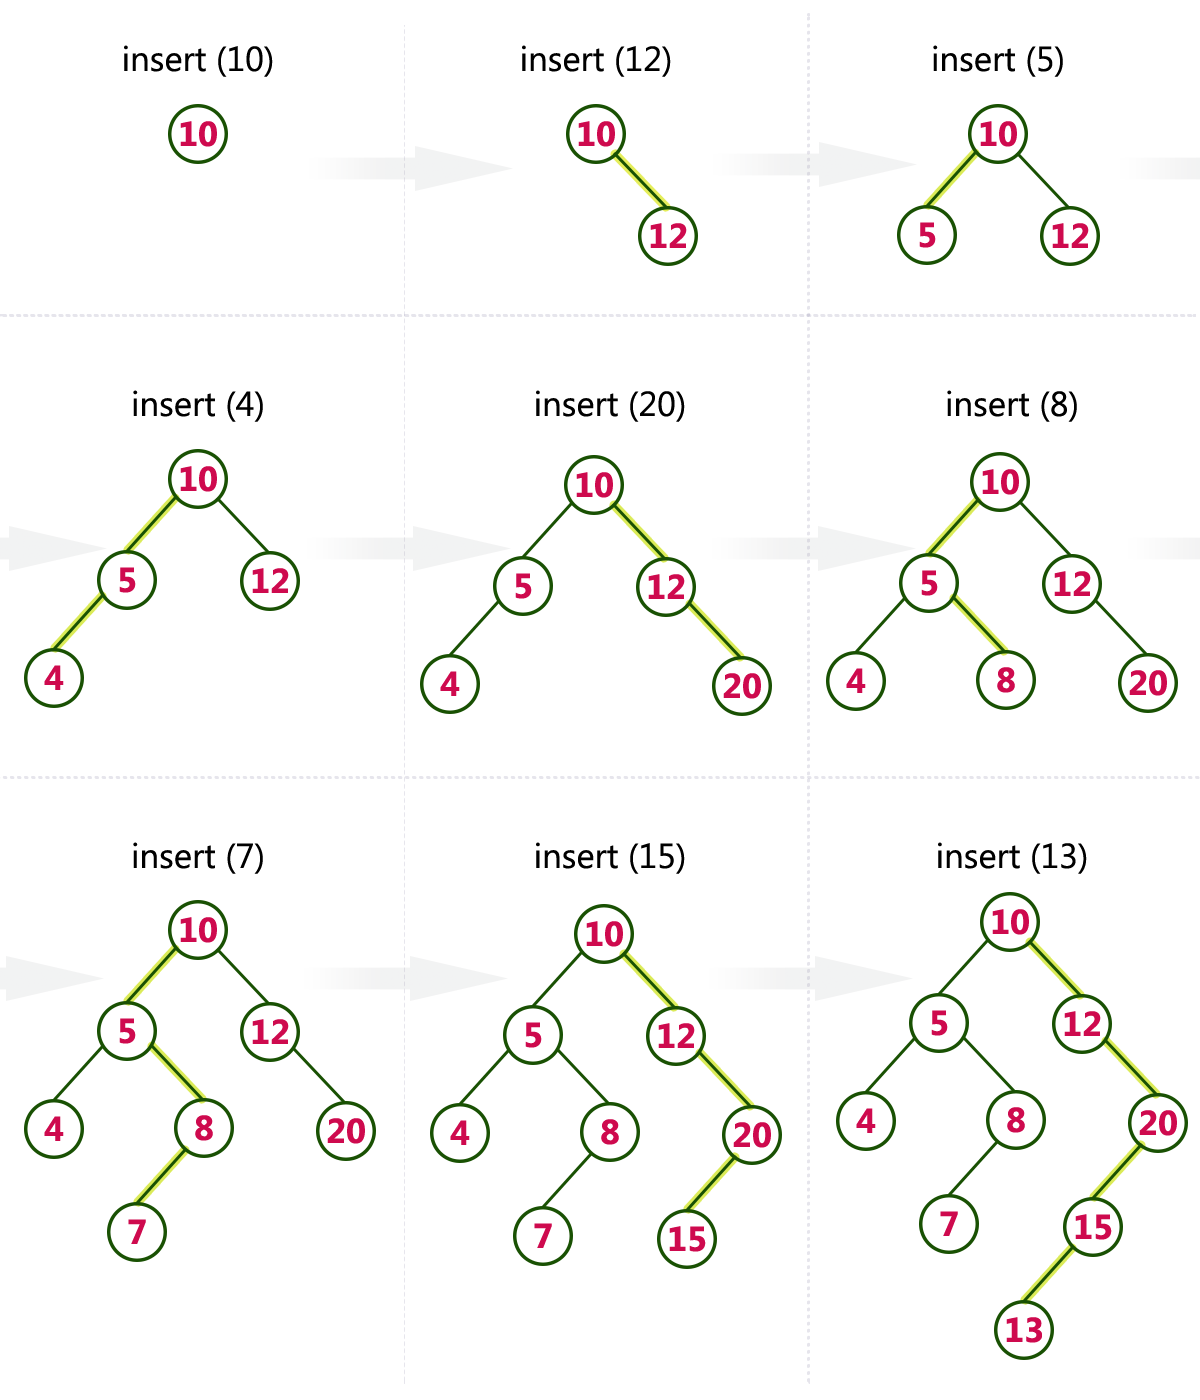
\includegraphics[width=0.4\textwidth]{assets/aula5-arvores5.png}
    \caption{Inspecionando os elementos de uma árvore}
  \end{figure}
\end{frame}
% Slide: Ordenação e Traversal
\begin{frame}[fragile]
  \frametitle{Ordenação e Traversal}
  \begin{itemize}
    \item \textbf{Traversal:} As árvores binárias suportam vários métodos de traversal (percurso), que determinam a ordem na qual os nós são visitados, incluindo:
      \begin{itemize}
        \item \textit{Preordem:} Visita primeiro a raiz, depois a subárvore esquerda, seguida da subárvore direita.
        \item \textit{Inordem:} Visita primeiro a subárvore esquerda, depois a raiz, e finalmente a subárvore direita
        \item \textit{Inordem:} Visita primeiro a subárvore esquerda, depois a raiz, e finalmente a subárvore direita. Este método resulta nos valores sendo visitados em ordem crescente, útil para obter os elementos da árvore ordenados.
        \item \textit{Pós-ordem:} Visita primeiro as subárvores esquerda e direita, e por último a raiz. É útil para operações que precisam processar um nó depois de seus descendentes, como liberar memória de uma árvore.
      \end{itemize}
  \end{itemize}
\end{frame}
% Slide: Ordenação e Traversal
\begin{frame}[fragile]
  \frametitle{Ordenação e Traversal}
  \begin{itemize}
    \item \textbf{Ordenação:}
      \begin{itemize}
        \item Através do traversal inordem, é possível extrair todos os elementos de uma árvore binária em ordem crescente.
        \item Este processo é especialmente útil para visualizar a estrutura de dados de uma maneira linear e ordenada, ou para realizar operações ordenadas sobre os dados.
      \end{itemize}
    \item \textbf{Importância do Traversal:} A escolha do método de traversal afeta diretamente a eficiência e o tipo de operações que podem ser realizadas em uma árvore. Por exemplo, o traversal inordem é essencial para operações de busca e ordenação, enquanto o pré-ordem e pós-ordem são importantes para reconstruir ou copiar a árvore.
  \end{itemize}
\end{frame}

% Slide: Exercício de Inserção em Árvores Binárias Não Balanceadas
\begin{frame}[fragile]
  \frametitle{Exercício de Inserção em Árvores Binárias Não Balanceadas}
  \begin{itemize}
    \item \textbf{Objetivo:} Praticar a inserção de valores em árvores binárias não balanceadas, observando como a estrutura da árvore se desenvolve com cada inserção.
    \item \textbf{Instruções:}
      \begin{enumerate}
        \item Comece com uma árvore vazia.
        \item Insira os valores do conjunto fornecido, um de cada vez, seguindo as regras de inserção para árvores binárias.
        \item Após cada inserção, desenhe a árvore resultante.
        \item Repita o processo para cada conjunto de valores fornecido.
      \end{enumerate}
  \end{itemize}
\end{frame}


% Slide: Exercício de Inserção em Árvores Binárias Não Balanceadas
\begin{frame}[fragile]
  \frametitle{Exercício de Inserção em Árvores Binárias Não Balanceadas}
  \begin{itemize}
    \item \textbf{Conjuntos de Valores:}
      \begin{itemize}
        \item \textit{Conjunto 1:} 11, 1, 14, 18, 2, 16, 6, 15, 13, 12
        \item \textit{Conjunto 2:} 5, 8, 7, 3, 16, 18, 14, 19, 15, 2
        \item \textit{Conjunto 3:} 2, 20, 5, 19, 13, 15, 11, 8, 4, 3
      \end{itemize}
    \item \textbf{Dica:} Lembre-se de que em uma árvore binária não balanceada, os valores menores que o nó atual devem ser inseridos à esquerda, e os valores maiores à direita.
    \item \textbf{Discussão:} Após a conclusão, discuta como as diferentes sequências de inserção afetam a forma e a altura da árvore. Qual conjunto resultou na árvore mais balanceada? E na mais desbalanceada?
  \end{itemize}
\end{frame}
\begin{frame}[fragile]
  \frametitle{Passos de Inserção em Árvores Binárias Não Balanceadas}
  
  \textit{Conjunto 1: Inserção passo a passo}

  \textbf{Inserir 11}\\
  Árvore vazia, apenas insere o 11 como raiz.
  
  \textbf{Inserir 1}\\
  Árvore não vazia. 1 < 11, insere à esquerda de 11.
  
  \textbf{Inserir 14}\\
  Árvore não vazia. 14 > 11, insere à direita de 11.
  
  \textbf{Inserir 18}\\
  Segue o caminho: 18 > 11, 18 > 14, insere à direita de 14.
  
\end{frame}
\begin{frame}[fragile]
  \frametitle{Passos de Inserção em Árvores Binárias Não Balanceadas}

  \textit{Conjunto 1: Inserção passo a passo}

  \textbf{Inserir 2}\\
  Segue o caminho: 2 < 11, insere à esquerda de 11. Como existe um nó 1, e 2 > 1, insere à direita de 1.

  \textbf{Inserir 16}\\
  Segue o caminho: 16 > 11, 16 > 14, insere à direita de 14. Como existe um nó 18, e 16 < 18, insere à esquerda de 18.

  \textbf{Inserir 6}\\
  Segue o caminho: 6 < 11, insere à esquerda de 11. Como existe um nó 1, e 6 > 1, insere à direita de 1. Como existe um nó 2, e 6 > 2, insere à direita de 2.


\end{frame}
\begin{frame}[fragile]
  \frametitle{Passos de Inserção em Árvores Binárias Não Balanceadas}

  \textit{Conjunto 1: Inserção passo a passo}

  \textbf{Inserir 15}\\
  Segue o caminho: 15 > 11, 15 > 14, insere à direita de 14. Como existe um nó 16, e 15 < 16, insere à esquerda de 16.

  \textbf{Inserir 13}\\
  Segue o caminho: 13 > 11, 13 < 14, insere à esquerda de 14.

  \textbf{Inserir 12}\\
  Segue o caminho: 12 > 11, 12 < 14, insere à esquerda de 14. Como existe um nó 13, e 12 < 13, insere à esquerda de 13.
\end{frame}
    
% \title{Arvores AVL}
\date{\today}
\frame{\titlepage}


\section{Arvores AVL}
\subsection{Introdução}
\begin{frame}[fragile]{\secname : \subsecname}

  \begin{itemize}
  \item A árvore AVL (nomeada por seus inventores Adelson-Velskii e Landis) deve ser vista como um BST com a seguinte propriedade adicional: 
  \begin{itemize}
  \item Para cada nó, as alturas de suas subárvores esquerda e direita diferem em no máximo 1.
  \end{itemize}
  \item Para concretizar a árvore AVL, precisamos definir uma propriedade constante para todas os nós.
\end{itemize}
\begin{equation}
\forall n: Node \bullet~|~altura(n.left) - altura(n.right)~| \leq 1
\end{equation}

  
\end{frame}
%%%%%%%%%%%%%%%%
%%% frame %%%%%%
%%%%%%%%%%%%%%%%

\begin{frame}[fragile]{\secname : \subsecname}

  \begin{itemize}
  \item Contanto que a árvore se mantenha esta propriedade, se a árvore contiver $n$ 
  nós, então ela terá uma profundidade de no máximo $O (log~n)$. 
  \end{itemize}
\end{frame}
%%%%%%%%%%%%%%%%
%%% frame %%%%%%
%%%%%%%%%%%%%%%%
\begin{frame}[fragile]{\secname : \subsecname}
  \begin{itemize}

  \item Como resultado, a busca por qualquer nó custará $O (log~n)$, e 
  se as atualizações puderem ser feitas em tempo proporcional à profundidade 
  do nó inserido ou excluído, então as atualizações também 
  custarão $O (log~n)$, mesmo no pior caso.
  \item Lembrando que $O (log~n) < O (n)$ 
  \end{itemize}
\end{frame}
%%%%%%%%%%%%%%%%
%%% frame %%%%%%
%%%%%%%%%%%%%%%%
\subsection{O que muda da BST?}
\begin{frame}[fragile]{\secname : \subsecname}

  \begin{itemize}
  \item A chave para fazer a árvore AVL funcionar é alterar as rotinas de 
  inserção e exclusão de modo a manter a propriedade de balanceamento. 
  \item Obviamente, para ser prático, devemos ser capazes de implementar as 
  rotinas de atualização revisadas em tempo $\Theta (log~n)$.
  \item Isso significa dizer, que o crescimento da complexidade em 
  relação ao tempo tem que ser exatamente $(log~n)$
  \end{itemize}
\end{frame}

%%%%%%%%%%%%%%%%
%%% frame %%%%%%
%%%%%%%%%%%%%%%%
\begin{frame}[fragile]{\secname : \subsecname}

  \begin{figure}[!h]
    \centering
    \caption{Inserir 5}
  
  \begin{tikzpicture}[->,>=stealth',
    % level/.style={sibling distance = 8cm/#1, level distance = 1.5cm},
    level 1/.style={sibling distance=15em, level distance = 3em},
    level 2/.style={sibling distance=8em, level distance = 3em},
    level 3/.style={sibling distance=5em, level distance = 3em},
    level 4/.style={sibling distance=3em, level distance = 3em},
    level 5/.style={sibling distance=2em, level distance = 3em} ]
    \node [wv] (r){37}
    child { node [wv] {24}
      child { node [gv] {7}
        child { node [gv] {2}
          child {node [nil] {}}
          child { node [rv] {5}
            child {node [nil] {}}
            child {node [nil] {}}
          }
        }
        child {node [nil] {}}
      }
      child { node [wv] {32}
        child {node [nil] {}}
        child {node [nil] {}}
      }
    }
    child { node [wv] {42}
      child { node [wv] {40}
        child {node [nil] {}}
        child {node [nil] {}}
      }
      child { node [wv] {45}
        child {node [nil] {}}
        child { node [wv] {120}
          child {node [nil] {}}
          child {node [nil] {}}
        }
      }
    }
    ;
  \end{tikzpicture}
  \end{figure}
\end{frame}
%%%%%%%%%%%%%%%% 
%%% frame %%%%%%
%%%%%%%%%%%%%%%%
\section{Desbalanceamento}
\subsection{Na AVL}
\begin{frame}[fragile]{\secname : \subsecname}
  \begin{itemize}
  \item Considere o que acontece quando inserimos um nó com valor de chave 5, 
  conforme mostrado na Figura do slide anterior. 
  \item A árvore à esquerda atende aos requisitos de balanceamento da árvore AVL. 
  \item Após a inserção, dois nós não atendem mais aos requisitos. 
  \item Como a árvore original atendeu ao requisito de balanceamento, os 
  nós na nova árvore só podem ser desbalanceados por uma \textbf{diferença de altura} de no 
  \textbf{máximo $\pm~2$} nas subárvores. 
  \end{itemize}
\end{frame}
%%%%%%%%%%%%%%%%
%%% frame %%%%%%
%%%%%%%%%%%%%%%%
\begin{frame}[fragile]{\secname : \subsecname}

  \begin{figure}[!h]
    \centering
    \caption{Inserir 5}
  
  \begin{tikzpicture}[->,>=stealth',
    % level/.style={sibling distance = 8cm/#1, level distance = 1.5cm},
    level 1/.style={sibling distance=15em, level distance = 3em},
    level 2/.style={sibling distance=8em, level distance = 3em},
    level 3/.style={sibling distance=5em, level distance = 3em},
    level 4/.style={sibling distance=3em, level distance = 3em},
    level 5/.style={sibling distance=2em, level distance = 3em}]
    \node [wv] (r){37}
    child { node [wv] {24}
      child { node [gv,label=above:-2] {7}
        child { node [gv,label=above:+1] {2}
          child {node [nil] {}}
          child { node [rv,label=above:0] {5}
            child {node [nil] {}}
            child {node [nil] {}}
          }
        }
        child {node [nil] {}}
      }
      child { node [wv] {32}
        child {node [nil] {}}
        child {node [nil] {}}
      }
    }
    child { node [wv] {42}
      child { node [wv] {40}
        child {node [nil] {}}
        child {node [nil] {}}
      }
      child { node [wv] {45}
        child {node [nil] {}}
        child { node [wv] {120}
          child {node [nil] {}}
          child {node [nil] {}}
        }
      }
    }
    ;
  \end{tikzpicture}
  \end{figure}
\end{frame}

%%%%%%%%%%%%%%%%
%%% frame %%%%%%
%%%%%%%%%%%%%%%%
\begin{frame}[fragile]{\secname : \subsecname}
  \begin{itemize}
  \item O desbalanceamento é causado pela diferença na altura dos nós
  \item Na aula passada vimos que a altura é calculada tomando como referência uma linha imaginária abaixo da árvore
  \item Para o nó mais inferior desbalanceado, chame-o de $S$, onde podemos ter 4 casos:
    \begin{itemize}
      \item[1.] O nó \textbf{filho} está no \textbf{filho esquerdo} da \emph{sub-árvore esquerda} de $S$.
      \item[2.] O nó \textbf{filho} está no \textbf{filho direito} da \emph{sub-árvore direita} de $S$.
      \item[3.] O nó \textbf{filho} está no \textbf{filho direito} da \emph{sub-árvore esquerda} de $S$. 
      \item[4.] O nó \textbf{filho} está no \textbf{filho esquerdo} da \emph{sub-árvore direita} de $S$. 
    \end{itemize}
  \end{itemize}
\end{frame}
%%%%%%%%%%%%%%%%
%%% frame %%%%%%
%%%%%%%%%%%%%%%%




\section{Rotações Simples}

%%%%%%
\subsection{À direita (RSD)}
%%%%%%
\begin{frame}[fragile]{\secname : \subsecname}
  O nó \textbf{filho} está no \textbf{filho esquerdo} da \emph{sub-árvore esquerda} de $S$.
  \begin{columns}[T] % align columns
    \begin{column}{.48\textwidth}
    \rule{\linewidth}{4pt}
    \begin{figure}[!h]
      \centering
      
    
    \begin{tikzpicture}[->,>=stealth',
      % level/.style={sibling distance = 8cm/#1, level distance = 1.5cm},
      level 1/.style={sibling distance=7em},
      level 2/.style={sibling distance=4em},
      level 3/.style={sibling distance=2em},
      level 4/.style={sibling distance=2em}]
    \node [wv] (r){8}
    child { node [wv] {6}
    child { node [rv] {4}
    child {node [nil] {A}}
    child {node [nil] {B}}
    }
    child {node [nil] {C}}
    }
    child {node [nil] {D}}
    ;
    \end{tikzpicture}
    \end{figure}
   
    \end{column}%
    \hfill%
    \begin{column}{.48\textwidth}
    \rule{\linewidth}{4pt}
          
        
    \begin{figure}[!h]
      \centering
      

    \begin{tikzpicture}[->,>=stealth',
      % level/.style={sibling distance = 8cm/#1, level distance = 1.5cm},
      level 1/.style={sibling distance=7em},
      level 2/.style={sibling distance=4em},
      level 3/.style={sibling distance=2em},
      level 4/.style={sibling distance=2em}]
    \node [wv] (r){6}
    child { node [wv] {4}
      child {node [nil] {A}}
      child {node [nil] {B}}
    }
    child { node [wv] {8}
      child {node [nil] {C}}
      child {node [nil] {D}}
    };
    \end{tikzpicture}
    \end{figure}
    \end{column}%
    \end{columns}

\end{frame}
%%%%%%%%%%%%%%%%
%%% frame %%%%%%
%%%%%%%%%%%%%%%%

\subsection{À esquerda (RSE)}
%%%%%%
\begin{frame}[fragile]{\secname : \subsecname}
  O nó \textbf{filho} está no \textbf{filho direito} da \emph{sub-árvore direita} de $S$.
  \begin{columns}[T] % align columns
    \begin{column}{.48\textwidth}
    \rule{\linewidth}{4pt}
    

      \begin{figure}[!h]
        \centering
        
      \begin{tikzpicture}[->,>=stealth',
        % level/.style={sibling distance = 8cm/#1, level distance = 1.5cm},
        level 1/.style={sibling distance=7em},
        level 2/.style={sibling distance=4em},
        level 3/.style={sibling distance=2em},
        level 4/.style={sibling distance=2em}]
      \node [wv] (r){4}
      child {node [nil] {A}}
      child { node [wv] {6}
          child {node [nil] {B}}
          child { node [rv] {8}
          child {node [nil] {C}}
          child {node [nil] {D}}
        }
      };
      \end{tikzpicture}
      \end{figure}
   
    \end{column}%
    \hfill%
    \begin{column}{.48\textwidth}
    \rule{\linewidth}{4pt}
          
        
      \begin{figure}[!h]
        \centering
        

      \begin{tikzpicture}[->,>=stealth',
        % level/.style={sibling distance = 8cm/#1, level distance = 1.5cm},
        level 1/.style={sibling distance=7em},
        level 2/.style={sibling distance=4em},
        level 3/.style={sibling distance=2em},
        level 4/.style={sibling distance=2em}]
      \node [wv] (r){6}
      child { node [wv] {4}
      child {node [nil] {A}}
      child {node [nil] {B}}
      }
      child { node [wv] {8}
      child {node [nil] {C}}
      child {node [nil] {D}}
      };
      \end{tikzpicture}
      \end{figure}
    \end{column}%
    \end{columns}

\end{frame}
%%%%%%%%%%%%%%%%
%%% frame %%%%%%
%%%%%%%%%%%%%%%%


\section{Rotações Duplas}

%%%%%%
\subsection{RSE + RSD = RED}
%%%%%%
\begin{frame}[fragile]{\secname : \subsecname}
  O nó \textbf{filho} está no \textbf{filho direito} da \emph{sub-árvore esquerda} de $S$. 
  \begin{columns}[T] % align columns
    \begin{column}{.31\textwidth}
    \rule{\linewidth}{4pt}
    
    \begin{figure}[!h]
      \centering
      
    \begin{tikzpicture}[->,>=stealth',
      % level/.style={sibling distance = 8cm/#1, level distance = 1.5cm},
      level 1/.style={sibling distance=7em},
      level 2/.style={sibling distance=4em},
      level 3/.style={sibling distance=2em},
      level 4/.style={sibling distance=2em}]
    \node [wv] (r){8}
    child { node [wv] {4}
            child {node [nil] {A}}
            child { node [rv] {6}
              child {node [nil] {B}}
              child {node [nil] {C}}
            }
    }
    child {node [nil] {D}};
    \end{tikzpicture}
    \caption{Aplicar RSE}
    \end{figure}
    \end{column}%
    \hfill%
    \begin{column}{.31\textwidth}
    \rule{\linewidth}{4pt}
    
    \begin{figure}[!h]
      \centering
      
    \begin{tikzpicture}[->,>=stealth',
      % level/.style={sibling distance = 8cm/#1, level distance = 1.5cm},
      level 1/.style={sibling distance=7em},
      level 2/.style={sibling distance=4em},
      level 3/.style={sibling distance=2em},
      level 4/.style={sibling distance=2em}]
      \node [wv] (r){8}
        child { node [wv] {6}
          child { node [wv] {4}
            child {node [nil] {A}}
            child {node [nil] {B}}
          }
          child {node [nil] {C}}
        }
        child {node [nil] {D}};
    \end{tikzpicture}
      \caption{Aplicar RSD}
    \end{figure}
    \end{column}%

    \hfill%
    \begin{column}{.31\textwidth}
    \color{black}\rule{\linewidth}{4pt}
    
    \begin{figure}[!h]
      \centering
      
      \begin{tikzpicture}[->,>=stealth',
        % level/.style={sibling distance = 8cm/#1, level distance = 1.5cm},
        level 1/.style={sibling distance=7em},
        level 2/.style={sibling distance=4em},
        level 3/.style={sibling distance=2em},
        level 4/.style={sibling distance=2em}]
      \node [wv] (r){6}
      child { node [wv] {4}
        child {node [nil] {A}}
        child {node [nil] {B}}
      }
      child { node [wv] {8}
        child {node [nil] {C}}
        child {node [nil] {D}}
      };
      \end{tikzpicture}
      \caption{Final}
    \end{figure}
    \end{column}%
    \end{columns}

\end{frame}
%%%%%%%%%%%%%%%%
%%% frame %%%%%%
%%%%%%%%%%%%%%%%

\subsection{RSD + RSE = RDE}

%%%%%%
\begin{frame}[fragile]{\secname : \subsecname}
  O nó \textbf{filho} está no \textbf{filho esquerdo} da \emph{sub-árvore direita} de $S$. 
  \begin{columns}[T] % align columns
    \begin{column}{.31\textwidth}
    \rule{\linewidth}{4pt}
    
    \begin{figure}[!h]
      \centering
      
    \begin{tikzpicture}[->,>=stealth',
      % level/.style={sibling distance = 8cm/#1, level distance = 1.5cm},
      level 1/.style={sibling distance=7em},
      level 2/.style={sibling distance=4em},
      level 3/.style={sibling distance=2em},
      level 4/.style={sibling distance=2em}]
    \node [wv] (r){4}
    child {node [nil] {A}}
    child { node [wv] {8}
      child { node [rv] {6}
        child {node [nil] {B}}
        child {node [nil] {C}}
      }
      child {node [nil] {D}}
    };
    \end{tikzpicture}
    \caption{Aplicar RSD}
    \end{figure}
    \end{column}%
    \hfill%
    \begin{column}{.31\textwidth}
    \rule{\linewidth}{4pt}
    
    \begin{figure}[!h]
      \centering
      
      \begin{tikzpicture}[->,>=stealth',
        % level/.style={sibling distance = 8cm/#1, level distance = 1.5cm},
        level 1/.style={sibling distance=7em},
        level 2/.style={sibling distance=4em},
        level 3/.style={sibling distance=2em},
        level 4/.style={sibling distance=2em}]
        \node [wv] (r){4}
        child {node [nil] {A}}
        child { node [wv] {6}
        child {node [nil] {B}}
        child { node [wv] {8}
        child {node [nil] {C}}
        child {node [nil] {D}}
        }
        };
      \end{tikzpicture}
      \caption{Aplicar RSE}
    \end{figure}
    \end{column}%
    \hfill%
    \begin{column}{.31\textwidth}
    \color{black}\rule{\linewidth}{4pt}
    
    \begin{figure}[!h]
      \centering
      

    \begin{tikzpicture}[->,>=stealth',
      % level/.style={sibling distance = 8cm/#1, level distance = 1.5cm},
      level 1/.style={sibling distance=7em},
      level 2/.style={sibling distance=4em},
      level 3/.style={sibling distance=2em},
      level 4/.style={sibling distance=2em}]
    \node [wv] (r){6}
    child { node [wv] {4}
      child {node [nil] {A}}
      child {node [nil] {B}}
    }
    child { node [wv] {8}
      child {node [nil] {C}}
      child {node [nil] {D}}
    };
    \end{tikzpicture}
    \caption{Final}
    \end{figure}
    \end{column}%
    \end{columns}

\end{frame}
%%%%%%%%%%%%%%%%
%%% frame %%%%%%
%%%%%%%%%%%%%%%%

\subsection{Exemplo 1}
\begin{frame}[fragile]{\secname : \subsecname}
  Inserir: \textbf{3}, 46, 41, 11, 42, 14, 10, 5, 24, 20, 31, 44, 48, 39, 21
\begin{figure}[!h]
  \centering
  \caption{Inserir 3}


\begin{tikzpicture}[->,>=stealth',
  % level/.style={sibling distance = 8cm/#1, level distance = 1.5cm},
 level 1/.style={sibling distance=15em, level distance = 3em},
  level 2/.style={sibling distance=8em, level distance = 3em},
  level 3/.style={sibling distance=4em, level distance = 3em},
  level 4/.style={sibling distance=2em, level distance = 3em},
  level 5/.style={sibling distance=1em, level distance = 3em} ]
\node [wv] (r){3}
child {node [nil] {}}
child {node [nil] {}};
\end{tikzpicture}

\end{figure}

\end{frame}


%%% frame


\begin{frame}[fragile]{\secname : \subsecname}
  Inserir: \textbf{3, 46}, 41, 11, 42, 14, 10, 5, 24, 20, 31, 44, 48, 39, 21
\begin{figure}[!h]
  \centering
  \caption{Inserir 46}



\begin{tikzpicture}[->,>=stealth',
  % level/.style={sibling distance = 8cm/#1, level distance = 1.5cm},
 level 1/.style={sibling distance=15em, level distance = 3em},
  level 2/.style={sibling distance=8em, level distance = 3em},
  level 3/.style={sibling distance=4em, level distance = 3em},
  level 4/.style={sibling distance=2em, level distance = 3em},
  level 5/.style={sibling distance=1em, level distance = 3em} ]
\node [wv] (r){3}

child {node [nil] {}}
child { node [wv] {46}
              child {node [nil] {}}
              child {node [nil] {}}
            };
\end{tikzpicture}
\end{figure}
\end{frame}


%%% frame


\begin{frame}[fragile]{\secname : \subsecname}
  Inserir: \textbf{3, 46, 41}, 11, 42, 14, 10, 5, 24, 20, 31, 44, 48, 39, 21

\begin{figure}[!h]
  \centering
  \caption{ Inserir 41}

\begin{tikzpicture}[->,>=stealth',
  % level/.style={sibling distance = 8cm/#1, level distance = 1.5cm},
 level 1/.style={sibling distance=15em, level distance = 3em},
  level 2/.style={sibling distance=8em, level distance = 3em},
  level 3/.style={sibling distance=4em, level distance = 3em},
  level 4/.style={sibling distance=2em, level distance = 3em},
  level 5/.style={sibling distance=1em, level distance = 3em} ]
\node [gv,label=above:+2] (r){3}
child {node [nil] {}}
child {node [gv,label=above:-1] {46}
              child { node [gv,label=above:0] {41}
                child {node [nil] {}}
                child {node [nil] {}}
              }
              child {node [nil] {}}
            };
\end{tikzpicture}

\end{figure}

\end{frame}


%%% frame


\begin{frame}[fragile]{\secname : \subsecname}
  Inserir: \textbf{3, 46, 41}, 11, 42, 14, 10, 5, 24, 20, 31, 44, 48, 39, 21
\begin{figure}[!h]
  \centering
  \caption{RSD 46 AR 41}

\begin{tikzpicture}[->,>=stealth',
  % level/.style={sibling distance = 8cm/#1, level distance = 1.5cm},
 level 1/.style={sibling distance=15em, level distance = 3em},
  level 2/.style={sibling distance=8em, level distance = 3em},
  level 3/.style={sibling distance=4em, level distance = 3em},
  level 4/.style={sibling distance=2em, level distance = 3em},
  level 5/.style={sibling distance=1em, level distance = 3em} ]
\node [gv,label=above:+2] (r){3}
child {node [nil] {}}
child {node [gv,label=above:+1] {41}
              child {node [nil] {}}
              child { node [gv,label=above:0] {46}
                child {node [nil] {}}
                child {node [nil] {}}
              }
            };
\end{tikzpicture}


\end{figure}

\end{frame}


%%% frame


\begin{frame}[fragile]{\secname : \subsecname}
  Inserir: \textbf{3, 46, 41}, 11, 42, 14, 10, 5, 24, 20, 31, 44, 48, 39, 21
\begin{figure}[!h]
  \centering
  \caption{RSE 3 AR 41}

\begin{tikzpicture}[->,>=stealth',
  % level/.style={sibling distance = 8cm/#1, level distance = 1.5cm},
 level 1/.style={sibling distance=15em, level distance = 3em},
  level 2/.style={sibling distance=8em, level distance = 3em},
  level 3/.style={sibling distance=4em, level distance = 3em},
  level 4/.style={sibling distance=2em, level distance = 3em},
  level 5/.style={sibling distance=1em, level distance = 3em} ]
\node [wv] (r){41}
child { node [wv] {3}
                child {node [nil] {}}
                child {node [nil] {}}
              }
child { node [wv] {46}
              child {node [nil] {}}
              child {node [nil] {}}
            };
\end{tikzpicture}

\end{figure}

\end{frame}


%%% frame


\begin{frame}[fragile]{\secname : \subsecname}
  Inserir: \textbf{3, 46, 41, 11}, 42, 14, 10, 5, 24, 20, 31, 44, 48, 39, 21
\begin{figure}[!h]
  \centering
  \caption{Inserir 11}

\begin{tikzpicture}[->,>=stealth',
  % level/.style={sibling distance = 8cm/#1, level distance = 1.5cm},
 level 1/.style={sibling distance=15em, level distance = 3em},
  level 2/.style={sibling distance=8em, level distance = 3em},
  level 3/.style={sibling distance=4em, level distance = 3em},
  level 4/.style={sibling distance=2em, level distance = 3em},
  level 5/.style={sibling distance=1em, level distance = 3em} ]
\node [wv] (r){41}
child { node [wv] {3}
                child {node [nil] {}}
                child { node [wv] {11}
                  child {node [nil] {}}
                  child {node [nil] {}}
              }
              }
child { node [wv] {46}
              child {node [nil] {}}
              child {node [nil] {}}
            };
\end{tikzpicture}


\end{figure}

\end{frame}


%%% frame


\begin{frame}[fragile]{\secname : \subsecname}
  Inserir: \textbf{3, 46, 41, 11, 42}, 14, 10, 5, 24, 20, 31, 44, 48, 39, 21
\begin{figure}[!h]
  \centering
  \caption{Inserir 42}

\begin{tikzpicture}[->,>=stealth',
  % level/.style={sibling distance = 8cm/#1, level distance = 1.5cm},
 level 1/.style={sibling distance=15em, level distance = 3em},
  level 2/.style={sibling distance=8em, level distance = 3em},
  level 3/.style={sibling distance=4em, level distance = 3em},
  level 4/.style={sibling distance=2em, level distance = 3em},
  level 5/.style={sibling distance=1em, level distance = 3em} ]
\node [wv] (r){41}
child { node [wv] {3}
                child {node [nil] {}}
                child { node [wv] {11}
                  child {node [nil] {}}
                  child {node [nil] {}}
              }
              }
child { node [wv] {46}
            child { node [wv] {42}
              child {node [nil] {}}
              child {node [nil] {}}
            }
              child {node [nil] {}}
            };
\end{tikzpicture}


\end{figure}

\end{frame}


%%% frame


\begin{frame}[fragile]{\secname : \subsecname}
  Inserir: \textbf{3, 46, 41, 11, 42, 14}, 10, 5, 24, 20, 31, 44, 48, 39, 21
\begin{figure}[!h]
  \centering
    \caption{Inserir 14}

\begin{tikzpicture}[->,>=stealth',
  % level/.style={sibling distance = 8cm/#1, level distance = 1.5cm},
 level 1/.style={sibling distance=15em, level distance = 3em},
  level 2/.style={sibling distance=8em, level distance = 3em},
  level 3/.style={sibling distance=4em, level distance = 3em},
  level 4/.style={sibling distance=2em, level distance = 3em},
  level 5/.style={sibling distance=1em, level distance = 3em} ]
\node [wv] (r){41}
child { node [gv,label=above:+2] {3}
                child {node [nil] {}}
                child { node [gv,label=above:+1] {11}
                  child {node [nil] {}}
                  child { node [gv,label=above:0] {14}
                      child {node [nil] {}}
                      child {node [nil] {}}
                  }
              }
              }
child { node [wv] {46}
            child { node [wv] {42}
              child {node [nil] {}}
              child {node [nil] {}}
            }
              child {node [nil] {}}
            };
\end{tikzpicture}


\end{figure}

\end{frame}


%%% frame


\begin{frame}[fragile]{\secname : \subsecname}
  Inserir: \textbf{3, 46, 41, 11, 42, 14}, 10, 5, 24, 20, 31, 44, 48, 39, 21
\begin{figure}[!h]
  \centering
    \caption{RSE 3 AR 11}

\begin{tikzpicture}[->,>=stealth',
  % level/.style={sibling distance = 8cm/#1, level distance = 1.5cm},
 level 1/.style={sibling distance=15em, level distance = 3em},
  level 2/.style={sibling distance=8em, level distance = 3em},
  level 3/.style={sibling distance=4em, level distance = 3em},
  level 4/.style={sibling distance=2em, level distance = 3em},
  level 5/.style={sibling distance=1em, level distance = 3em} ]
\node [wv] (r){41}
child { node [wv] {11}
            child { node [wv] {3}
              child {node [nil] {}}
              child {node [nil] {}}
            } child { node [wv] {14}
              child {node [nil] {}}
              child {node [nil] {}}
            }
      }
child { node [wv] {46}
            child { node [wv] {42}
              child {node [nil] {}}
              child {node [nil] {}}
            }
              child {node [nil] {}}
      };
\end{tikzpicture}

\end{figure}

\end{frame}


%%% frame


\begin{frame}[fragile]{\secname : \subsecname}
  Inserir: \textbf{3, 46, 41, 11, 42, 14, 10}, 5, 24, 20, 31, 44, 48, 39, 21
\begin{figure}[!h]
  \centering
    \caption{Inserir 10}

\begin{tikzpicture}[->,>=stealth',
  % level/.style={sibling distance = 8cm/#1, level distance = 1.5cm},
 level 1/.style={sibling distance=15em, level distance = 3em},
  level 2/.style={sibling distance=8em, level distance = 3em},
  level 3/.style={sibling distance=4em, level distance = 3em},
  level 4/.style={sibling distance=2em, level distance = 3em},
  level 5/.style={sibling distance=1em, level distance = 3em} ]
\node [wv] (r){41}
child { node [wv] {11}
            child { node [wv] {3}
              child {node [nil] {}}
              child { node [wv] {10}
                child {node [nil] {}}
                child {node [nil] {}}
              } 
            } 
            child { node [wv] {14}
              child {node [nil] {}}
              child {node [nil] {}}
            }
      }
child { node [wv] {46}
            child { node [wv] {42}
              child {node [nil] {}}
              child {node [nil] {}}
            }
              child {node [nil] {}}
      };
\end{tikzpicture}

\end{figure}

\end{frame}


%%% frame


\begin{frame}[fragile]{\secname : \subsecname}
  Inserir: \textbf{3, 46, 41, 11, 42, 14, 10, 5}, 24, 20, 31, 44, 48, 39, 21

\begin{figure}[!h]
  \centering
    \caption{Inserir 5}

\begin{tikzpicture}[->,>=stealth',
  % level/.style={sibling distance = 8cm/#1, level distance = 1.5cm},
 level 1/.style={sibling distance=15em, level distance = 3em},
  level 2/.style={sibling distance=8em, level distance = 3em},
  level 3/.style={sibling distance=4em, level distance = 3em},
  level 4/.style={sibling distance=2em, level distance = 3em},
  level 5/.style={sibling distance=1em, level distance = 3em} ]
\node [wv] (r){41}
child { node [wv] {11}
            child { node [gv,label=above:+2] {3}
              child {node [nil] {}}
              child { node [gv,label=above:-1] {10}
                child { node [gv,label=above:0] {5}
                  child {node [nil] {}}
                  child {node [nil] {}}
                }
                child {node [nil] {}}
              } 
            } 
            child { node [wv] {14}
              child {node [nil] {}}
              child {node [nil] {}}
            }
      }
child { node [wv] {46}
            child { node [wv] {42}
              child {node [nil] {}}
              child {node [nil] {}}
            }
              child {node [nil] {}}
      };
\end{tikzpicture}

\end{figure}

\end{frame}


%%% frame


\begin{frame}[fragile]{\secname : \subsecname}
  Inserir: \textbf{3, 46, 41, 11, 42, 14, 10, 5}, 24, 20, 31, 44, 48, 39, 21

\begin{figure}[!h]
  \centering
    \caption{RSD 10 AR 5 + RSE 3 AR 5}

\begin{tikzpicture}[->,>=stealth',
  % level/.style={sibling distance = 8cm/#1, level distance = 1.5cm},
 level 1/.style={sibling distance=15em, level distance = 3em},
  level 2/.style={sibling distance=8em, level distance = 3em},
  level 3/.style={sibling distance=4em, level distance = 3em},
  level 4/.style={sibling distance=2em, level distance = 3em},
  level 5/.style={sibling distance=1em, level distance = 3em} ]
\node [wv] (r){41}
child { node [wv] {11}
            child { node [wv] {5}
              child { node [wv] {3}
                child {node [nil] {}}
                child {node [nil] {}}
              }
              child { node [wv] {10}
                child {node [nil] {}}
                child {node [nil] {}}
              }
            }
            child { node [wv] {14}
              child {node [nil] {}}
              child {node [nil] {}}
            }
      }
child { node [wv] {46}
            child { node [wv] {42}
              child {node [nil] {}}
              child {node [nil] {}}
            }
              child {node [nil] {}}
      };
\end{tikzpicture}

\end{figure}

\end{frame}


%%% frame


\begin{frame}[fragile]{\secname : \subsecname}
  Inserir: \textbf{3, 46, 41, 11, 42, 14, 10, 5, 24}, 20, 31, 44, 48, 39, 21


\begin{figure}[!h]
  \centering
    \caption{Inserir 24}

\begin{tikzpicture}[->,>=stealth',
  % level/.style={sibling distance = 8cm/#1, level distance = 1.5cm},
 level 1/.style={sibling distance=15em, level distance = 3em},
  level 2/.style={sibling distance=8em, level distance = 3em},
  level 3/.style={sibling distance=4em, level distance = 3em},
  level 4/.style={sibling distance=2em, level distance = 3em},
  level 5/.style={sibling distance=1em, level distance = 3em} ]
\node [wv] (r){41}
child { node [wv] {11}
            child { node [wv] {5}
              child { node [wv] {3}
                child {node [nil] {}}
                child {node [nil] {}}
              }
              child { node [wv] {10}
                child {node [nil] {}}
                child {node [nil] {}}
              }
            }
            child { node [wv] {14}
              child {node [nil] {}}
              child { node [wv] {24}
                child {node [nil] {}}
                child {node [nil] {}}
              }
            }
      }
child { node [wv] {46}
            child { node [wv] {42}
              child {node [nil] {}}
              child {node [nil] {}}
            }
              child {node [nil] {}}
      };
\end{tikzpicture}

\end{figure}

\end{frame}


%%% frame


\begin{frame}[fragile]{\secname : \subsecname}
  Inserir: \textbf{3, 46, 41, 11, 42, 14, 10, 5, 24, 20}, 31, 44, 48, 39, 21

\begin{figure}[!h]
  \centering
    \caption{Inserir 20}

\begin{tikzpicture}[->,>=stealth',
  % level/.style={sibling distance = 8cm/#1, level distance = 1.5cm},
 level 1/.style={sibling distance=15em, level distance = 3em},
  level 2/.style={sibling distance=8em, level distance = 3em},
  level 3/.style={sibling distance=4em, level distance = 3em},
  level 4/.style={sibling distance=2em, level distance = 3em},
  level 5/.style={sibling distance=1em, level distance = 3em} ]
\node [wv] (r){41}
child { node [wv] {11}
            child { node [wv] {5}
              child { node [wv] {3}
                child {node [nil] {}}
                child {node [nil] {}}
              }
              child { node [wv] {10}
                child {node [nil] {}}
                child {node [nil] {}}
              }
            }
            child { node [gv,label=above:+2] {14}
              child {node [nil] {}}
              child { node [gv,label=above:-1] {24}
                child { node [gv,label=above:0] {20}
                  child {node [nil] {}}
                  child {node [nil] {}}
                }
                child {node [nil] {}}
              }
            }
      }
child { node [wv] {46}
            child { node [wv] {42}
              child {node [nil] {}}
              child {node [nil] {}}
            }
              child {node [nil] {}}
      };
\end{tikzpicture}

\end{figure}

\end{frame}


%%% frame


\begin{frame}[fragile]{\secname : \subsecname}
  Inserir: \textbf{3, 46, 41, 11, 42, 14, 10, 5, 24, 20}, 31, 44, 48, 39, 21

\begin{figure}[!h]
  \centering
    \caption{RSD 24 AR 20 + RSE 14 AR 20}

\begin{tikzpicture}[->,>=stealth',
  % level/.style={sibling distance = 8cm/#1, level distance = 1.5cm},
 level 1/.style={sibling distance=15em, level distance = 3em},
  level 2/.style={sibling distance=8em, level distance = 3em},
  level 3/.style={sibling distance=4em, level distance = 3em},
  level 4/.style={sibling distance=2em, level distance = 3em},
  level 5/.style={sibling distance=1em, level distance = 3em} ]
\node [wv] (r){41}
child { node [wv] {11}
            child { node [wv] {5}
              child { node [wv] {3}
                child {node [nil] {}}
                child {node [nil] {}}
              }
              child { node [wv] {10}
                child {node [nil] {}}
                child {node [nil] {}}
              }
            }
            child { node [wv] {20}
              child { node [wv] {14}
                child {node [nil] {}}
                child {node [nil] {}}
              }
              child { node [wv] {24}
                child {node [nil] {}}
                child {node [nil] {}}
              }
            }
      }
child { node [wv] {46}
            child { node [wv] {42}
              child {node [nil] {}}
              child {node [nil] {}}
            }
              child {node [nil] {}}
      };
\end{tikzpicture}

\end{figure}

\end{frame}


%%% frame


\begin{frame}[fragile]{\secname : \subsecname}
  Inserir: \textbf{3, 46, 41, 11, 42, 14, 10, 5, 24, 20, 31}, 44, 48, 39, 21
\begin{figure}[!h]
  \centering
    \caption{Inserir 31}

\begin{tikzpicture}[->,>=stealth',
  % level/.style={sibling distance = 8cm/#1, level distance = 1.5cm},
 level 1/.style={sibling distance=15em, level distance = 3em},
  level 2/.style={sibling distance=8em, level distance = 3em},
  level 3/.style={sibling distance=4em, level distance = 3em},
  level 4/.style={sibling distance=2em, level distance = 3em},
  level 5/.style={sibling distance=1em, level distance = 3em} ]
\node [gv,label=above:-2] (r){41}
child { node [gv,label=above:+1] {11}
            child { node [wv] {5}
              child { node [wv] {3}
                child {node [nil] {}}
                child {node [nil] {}}
              }
              child { node [wv] {10}
                child {node [nil] {}}
                child {node [nil] {}}
              }
            }
            child { node [gv,label=above:+1] {20}
              child { node [wv] {14}
                child {node [nil] {}}
                child {node [nil] {}}
              }
              child { node [wv,label=above:+1] {24}
                child {node [nil] {}}
                child { node [wv,label=above:0] {31}
                  child {node [nil] {}}
                  child {node [nil] {}}
                }
              }
            }
      }
child { node [wv] {46}
            child { node [wv] {42}
              child {node [nil] {}}
              child {node [nil] {}}
            }
              child {node [nil] {}}
      };
\end{tikzpicture}

\end{figure}

\end{frame}


%%% frame


\begin{frame}[fragile]{\secname : \subsecname}
  Inserir: \textbf{3, 46, 41, 11, 42, 14, 10, 5, 24, 20, 31}, 44, 48, 39, 21
\begin{figure}[!h]
  \centering
    \caption{RSE 11 AR 41 + RSD 41 AR 20}

\begin{tikzpicture}[->,>=stealth',
  % level/.style={sibling distance = 8cm/#1, level distance = 1.5cm},
 level 1/.style={sibling distance=15em, level distance = 3em},
  level 2/.style={sibling distance=8em, level distance = 3em},
  level 3/.style={sibling distance=4em, level distance = 3em},
  level 4/.style={sibling distance=2em, level distance = 3em},
  level 5/.style={sibling distance=1em, level distance = 3em} ]
\node [wv] (r){20}
child { node [wv] {11}
  child { node [wv] {5}
    child { node [wv] {3}
      child {node [nil] {}}
      child {node [nil] {}}
    }
    child { node [wv] {10}
      child {node [nil] {}}
      child {node [nil] {}}
    }
  }
  child { node [wv] {14}
    child {node [nil] {}}
    child {node [nil] {}}
  }
}
child { node [wv] {41}
  child { node [wv] {24}
    child {node [nil] {}}
    child { node [wv] {31}
      child {node [nil] {}}
      child {node [nil] {}}
    }
  }
  child { node [wv] {46}
    child { node [wv] {42}
      child {node [nil] {}}
      child {node [nil] {}}  
    }
    child {node [nil] {}}
  }
};
\end{tikzpicture}

\end{figure}

\end{frame}


%%% frame


\begin{frame}[fragile]{\secname : \subsecname}
  Inserir: \textbf{3, 46, 41, 11, 42, 14, 10, 5, 24, 20, 31, 44}, 48, 39, 21

\begin{figure}[!h]
  \centering
    \caption{Inserir 44}

\begin{tikzpicture}[->,>=stealth',
  % level/.style={sibling distance = 8cm/#1, level distance = 1.5cm},
 level 1/.style={sibling distance=15em, level distance = 3em},
  level 2/.style={sibling distance=8em, level distance = 3em},
  level 3/.style={sibling distance=4em, level distance = 3em},
  level 4/.style={sibling distance=2em, level distance = 3em},
  level 5/.style={sibling distance=1em, level distance = 3em} ]
\node [wv] (r){20}
child { node [wv] {11}
  child { node [wv] {5}
    child { node [wv] {3}
      child {node [nil] {}}
      child {node [nil] {}}
    }
    child { node [wv] {10}
      child {node [nil] {}}
      child {node [nil] {}}
    }
  }
  child { node [wv] {14}
    child {node [nil] {}}
    child {node [nil] {}}
  }
}
child { node [wv] {41}
  child { node [wv] {24}
    child {node [nil] {}}
    child { node [wv] {31}
      child {node [nil] {}}
      child {node [nil] {}}
    }
  }
  child { node [gv,label=above:-2] {46}
    child { node [gv,label=above:+1] {42}
      child {node [nil] {}}
      child { node [gv,label=above:0] {44}
        child {node [nil] {}}
        child {node [nil] {}}  
      }
    }
    child {node [nil] {}}
  }
};
\end{tikzpicture}

\end{figure}

\end{frame}


%%% frame


\begin{frame}[fragile]{\secname : \subsecname}
  Inserir: \textbf{3, 46, 41, 11, 42, 14, 10, 5, 24, 20, 31, 44}, 48, 39, 21


\begin{figure}[!h]
  \centering
    \caption{RSE 42 AR 44 + RSD 46 AR 44}

\begin{tikzpicture}[->,>=stealth',
  % level/.style={sibling distance = 8cm/#1, level distance = 1.5cm},
 level 1/.style={sibling distance=15em, level distance = 3em},
  level 2/.style={sibling distance=8em, level distance = 3em},
  level 3/.style={sibling distance=4em, level distance = 3em},
  level 4/.style={sibling distance=2em, level distance = 3em},
  level 5/.style={sibling distance=1em, level distance = 3em} ]
\node [wv] (r){20}
child { node [wv] {11}
  child { node [wv] {5}
    child { node [wv] {3}
      child {node [nil] {}}
      child {node [nil] {}}
    }
    child { node [wv] {10}
      child {node [nil] {}}
      child {node [nil] {}}
    }
  }
  child { node [wv] {14}
    child {node [nil] {}}
    child {node [nil] {}}
  }
}
child { node [wv] {41}
  child { node [wv] {24}
    child {node [nil] {}}
    child { node [wv] {31}
      child {node [nil] {}}
      child {node [nil] {}}
    }
  }
  child { node [wv] {44}
    child { node [wv] {42}
      child {node [nil] {}}
      child {node [nil] {}}
    }
    child { node [wv] {46}
      child {node [nil] {}}
      child {node [nil] {}}
    }
  }
};
\end{tikzpicture}

\end{figure}

\end{frame}


%%% frame


\begin{frame}[fragile]{\secname : \subsecname}
  Inserir: \textbf{3, 46, 41, 11, 42, 14, 10, 5, 24, 20, 31, 44, 48}, 39, 21
\begin{figure}[!h]
  \centering
    \caption{Inserir 48}

\begin{tikzpicture}[->,>=stealth',
  % level/.style={sibling distance = 8cm/#1, level distance = 1.5cm},
 level 1/.style={sibling distance=15em, level distance = 3em},
  level 2/.style={sibling distance=8em, level distance = 3em},
  level 3/.style={sibling distance=4em, level distance = 3em},
  level 4/.style={sibling distance=2em, level distance = 3em},
  level 5/.style={sibling distance=1em, level distance = 3em} ]
\node [wv] (r){20}
child { node [wv] {11}
  child { node [wv] {5}
    child { node [wv] {3}
      child {node [nil] {}}
      child {node [nil] {}}
    }
    child { node [wv] {10}
      child {node [nil] {}}
      child {node [nil] {}}
    }
  }
  child { node [wv] {14}
    child {node [nil] {}}
    child {node [nil] {}}
  }
}
child { node [wv] {41}
  child { node [wv] {24}
    child {node [nil] {}}
    child { node [wv] {31}
      child {node [nil] {}}
      child {node [nil] {}}
    }
  }
  child { node [wv] {44}
    child { node [wv] {42}
      child {node [nil] {}}
      child {node [nil] {}}
    }
    child { node [wv] {46}
      child {node [nil] {}}
      child { node [wv] {48}
        child {node [nil] {}}
        child {node [nil] {}}
      }
    }
  }
};
\end{tikzpicture}

\end{figure}

\end{frame}


%%% frame


\begin{frame}[fragile]{\secname : \subsecname}
  Inserir: \textbf{3, 46, 41, 11, 42, 14, 10, 5, 24, 20, 31, 44, 48, 39}, 21
  \begin{figure}[!h]
  \centering
    \caption{Inserir 39}

\begin{tikzpicture}[->,>=stealth',
  % level/.style={sibling distance = 8cm/#1, level distance = 1.5cm},
 level 1/.style={sibling distance=15em, level distance = 3em},
  level 2/.style={sibling distance=8em, level distance = 3em},
  level 3/.style={sibling distance=4em, level distance = 3em},
  level 4/.style={sibling distance=2em, level distance = 3em},
  level 5/.style={sibling distance=1em, level distance = 3em} ]
\node [wv] (r){20}
child { node [wv] {11}
  child { node [wv] {5}
    child { node [wv] {3}
      child {node [nil] {}}
      child {node [nil] {}}
    }
    child { node [wv] {10}
      child {node [nil] {}}
      child {node [nil] {}}
    }
  }
  child { node [wv] {14}
    child {node [nil] {}}
    child {node [nil] {}}
  }
}
child { node [wv] {41}
  child { node [gv,label=above:+2] {24}
    child {node [nil] {}}
    child { node [gv,label=above:+1] {31}
      child {node [nil] {}}
      child { node [gv,label=above:0] {39}
        child {node [nil] {}}
        child {node [nil] {}}
      }
    }
  }
  child { node [wv] {44}
    child { node [wv] {42}
      child {node [nil] {}}
      child {node [nil] {}}
    }
    child { node [wv] {46}
      child {node [nil] {}}
      child { node [wv] {48}
        child {node [nil] {}}
        child {node [nil] {}}
      }
    }
  }
};
\end{tikzpicture}

\end{figure}

\end{frame}


%%% frame


\begin{frame}[fragile]{\secname : \subsecname}
  Inserir: \textbf{3, 46, 41, 11, 42, 14, 10, 5, 24, 20, 31, 44, 48, 39}, 21
\begin{figure}[!h]
  \centering
    \caption{RSE 24 AR 31}

\begin{tikzpicture}[->,>=stealth',
  % level/.style={sibling distance = 8cm/#1, level distance = 1.5cm},
 level 1/.style={sibling distance=15em, level distance = 3em},
  level 2/.style={sibling distance=8em, level distance = 3em},
  level 3/.style={sibling distance=4em, level distance = 3em},
  level 4/.style={sibling distance=2em, level distance = 3em},
  level 5/.style={sibling distance=1em, level distance = 3em} ]
\node [wv] (r){20}
child { node [wv] {11}
  child { node [wv] {5}
    child { node [wv] {3}
      child {node [nil] {}}
      child {node [nil] {}}
    }
    child { node [wv] {10}
      child {node [nil] {}}
      child {node [nil] {}}
    }
  }
  child { node [wv] {14}
    child {node [nil] {}}
    child {node [nil] {}}
  }
}
child { node [wv] {41}
child { node [wv] {31}
  child { node [wv] {24}
      child {node [nil] {}}
      child {node [nil] {}}
    }
    child { node [wv] {39}
      child {node [nil] {}}
      child {node [nil] {}}
    } 
  }
  child { node [wv] {44}
    child { node [wv] {42}
      child {node [nil] {}}
      child {node [nil] {}}
    }
    child { node [wv] {46}
      child {node [nil] {}}
      child { node [wv] {48}
        child {node [nil] {}}
        child {node [nil] {}}
      }
    }
  }
};
\end{tikzpicture}

\end{figure}

\end{frame}


%%% frame


\begin{frame}[fragile]{\secname : \subsecname}
  Inserir: \textbf{3, 46, 41, 11, 42, 14, 10, 5, 24, 20, 31, 44, 48, 39, 21}
  \begin{figure}[!h]
  \centering
    \caption{Inserir 21}

\begin{tikzpicture}[->,>=stealth',
  % level/.style={sibling distance = 8cm/#1, level distance = 1.5cm},
 level 1/.style={sibling distance=15em, level distance = 3em},
  level 2/.style={sibling distance=8em, level distance = 3em},
  level 3/.style={sibling distance=4em, level distance = 3em},
  level 4/.style={sibling distance=2em, level distance = 3em},
  level 5/.style={sibling distance=1em, level distance = 3em} ]
\node [wv] (r){20}
child { node [wv] {11}
  child { node [wv] {5}
    child { node [wv] {3}
      child {node [nil] {}}
      child {node [nil] {}}
    }
    child { node [wv] {10}
      child {node [nil] {}}
      child {node [nil] {}}
    }
  }
  child { node [wv] {14}
    child {node [nil] {}}
    child {node [nil] {}}
  }
}
child { node [wv] {41}
child { node [wv] {31}
  child { node [wv] {24}
      child { node [wv] {21}
        child {node [nil] {}}
        child {node [nil] {}}
      }
      child {node [nil] {}}
    }
    child { node [wv] {39}
      child {node [nil] {}}
      child {node [nil] {}}
    } 
  }
  child { node [wv] {44}
    child { node [wv] {42}
      child {node [nil] {}}
      child {node [nil] {}}
    }
    child { node [wv] {46}
      child {node [nil] {}}
      child { node [wv] {48}
        child {node [nil] {}}
        child {node [nil] {}}
      }
    }
  }
};
\end{tikzpicture}

\end{figure}
\end{frame}


\subsection{Exemplo 2}
\begin{frame}[fragile] {\secname : \subsecname}
  Inserir: \textbf{4}, 39, 30, 27, 41, 46, 47, 10, 31, 8, 17, 12, 50, 2, 14
\begin{figure}[!h]
  \centering
  \caption{ Inserir 4 }

\begin{tikzpicture}[->,>=stealth',
  % level/.style={sibling distance = 8cm/#1, level distance = 1.5cm},
 level 1/.style={sibling distance=15em, level distance = 3em},
  level 2/.style={sibling distance=8em, level distance = 3em},
  level 3/.style={sibling distance=4em, level distance = 3em},
  level 4/.style={sibling distance=2em, level distance = 3em},
  level 5/.style={sibling distance=1em, level distance = 3em} ]
\node [wv] (r){4}
child {node [nil] {}}
child {node [nil] {}};
\end{tikzpicture}
\end{figure}
\end{frame}

%%%


\begin{frame}[fragile] {\secname : \subsecname}
  Inserir: \textbf{4, 39}, 30, 27, 41, 46, 47, 10, 31, 8, 17, 12, 50, 2, 14
\begin{figure}[!h]
  \centering
  \caption{ Inserir 39}

\begin{tikzpicture}[->,>=stealth',
  % level/.style={sibling distance = 8cm/#1, level distance = 1.5cm},
 level 1/.style={sibling distance=15em, level distance = 3em},
  level 2/.style={sibling distance=8em, level distance = 3em},
  level 3/.style={sibling distance=4em, level distance = 3em},
  level 4/.style={sibling distance=2em, level distance = 3em},
  level 5/.style={sibling distance=1em, level distance = 3em} ]
\node [wv] (r){4}

child {node [nil] {}}
child { node [wv] {39}
              child {node [nil] {}}
              child {node [nil] {}}
            };
\end{tikzpicture}

\end{figure}
\end{frame}

%%%


\begin{frame}[fragile] {\secname : \subsecname}
  Inserir: \textbf{4, 39, 30}, 27, 41, 46, 47, 10, 31, 8, 17, 12, 50, 2, 14
\begin{figure}[!h]
  \centering
  \caption{Inserir 30}

\begin{tikzpicture}[->,>=stealth',
  % level/.style={sibling distance = 8cm/#1, level distance = 1.5cm},
 level 1/.style={sibling distance=15em, level distance = 3em},
  level 2/.style={sibling distance=8em, level distance = 3em},
  level 3/.style={sibling distance=4em, level distance = 3em},
  level 4/.style={sibling distance=2em, level distance = 3em},
  level 5/.style={sibling distance=1em, level distance = 3em} ]
\node [gv,label=above:+2] (r){4}
child {node [nil] {}}
child {node [gv,label=above:-1] {39}
              child { node [gv,label=above:0] {30}
                child {node [nil] {}}
                child {node [nil] {}}
              }
              child {node [nil] {}}
            };
\end{tikzpicture}
\end{figure}
\end{frame}

%%%


\begin{frame}[fragile] {\secname : \subsecname}
  Inserir: \textbf{4, 39, 30}, 27, 41, 46, 47, 10, 31, 8, 17, 12, 50, 2, 14
\begin{figure}[!h]
  \centering
  \caption{ RSD 39 AR 30 }

\begin{tikzpicture}[->,>=stealth',
  % level/.style={sibling distance = 8cm/#1, level distance = 1.5cm},
 level 1/.style={sibling distance=15em, level distance = 3em},
  level 2/.style={sibling distance=8em, level distance = 3em},
  level 3/.style={sibling distance=4em, level distance = 3em},
  level 4/.style={sibling distance=2em, level distance = 3em},
  level 5/.style={sibling distance=1em, level distance = 3em} ]
\node [gv,label=above:+2] (r){4}
child {node [nil] {}}
child {node [gv,label=above:+1] {30}
              child {node [nil] {}}
              child { node [gv,label=above:0] {39}
                child {node [nil] {}}
                child {node [nil] {}}
              }
            };
\end{tikzpicture}
\end{figure}
\end{frame}

%%%


\begin{frame}[fragile] {\secname : \subsecname}
  Inserir: \textbf{4, 39, 30}, 27, 41, 46, 47, 10, 31, 8, 17, 12, 50, 2, 14
\begin{figure}[!h]
  \centering
  \caption{RSE 4 AR 30}

\begin{tikzpicture}[->,>=stealth',
  % level/.style={sibling distance = 8cm/#1, level distance = 1.5cm},
 level 1/.style={sibling distance=15em, level distance = 3em},
  level 2/.style={sibling distance=8em, level distance = 3em},
  level 3/.style={sibling distance=4em, level distance = 3em},
  level 4/.style={sibling distance=2em, level distance = 3em},
  level 5/.style={sibling distance=1em, level distance = 3em} ]
\node [wv] (r){30}
child { node [wv] {4}
                child {node [nil] {}}
                child {node [nil] {}}
              }
child { node [wv] {39}
              child {node [nil] {}}
              child {node [nil] {}}
            };
\end{tikzpicture}

\end{figure}
\end{frame}

%%%


\begin{frame}[fragile] {\secname : \subsecname}
  Inserir: \textbf{4, 39, 30, 27}, 41, 46, 47, 10, 31, 8, 17, 12, 50, 2, 14
\begin{figure}[!h]
  \centering
  \caption{Inserir 27}

\begin{tikzpicture}[->,>=stealth',
  % level/.style={sibling distance = 8cm/#1, level distance = 1.5cm},
 level 1/.style={sibling distance=15em, level distance = 3em},
  level 2/.style={sibling distance=8em, level distance = 3em},
  level 3/.style={sibling distance=4em, level distance = 3em},
  level 4/.style={sibling distance=2em, level distance = 3em},
  level 5/.style={sibling distance=1em, level distance = 3em} ]
\node [wv] (r){30}
child { node [wv] {4}
                child {node [nil] {}}
                child { node [wv] {27}
                  child {node [nil] {}}
                  child {node [nil] {}}
                }
              }
child { node [wv] {39}
              child {node [nil] {}}
              child {node [nil] {}}
            };
\end{tikzpicture}

\end{figure}
\end{frame}

%%%


\begin{frame}[fragile] {\secname : \subsecname}
  Inserir: \textbf{4, 39, 30, 27, 41}, 46, 47, 10, 31, 8, 17, 12, 50, 2, 14
\begin{figure}[!h]
  \centering
  \caption{Inserir 41}

\begin{tikzpicture}[->,>=stealth',
  % level/.style={sibling distance = 8cm/#1, level distance = 1.5cm},
 level 1/.style={sibling distance=15em, level distance = 3em},
  level 2/.style={sibling distance=8em, level distance = 3em},
  level 3/.style={sibling distance=4em, level distance = 3em},
  level 4/.style={sibling distance=2em, level distance = 3em},
  level 5/.style={sibling distance=1em, level distance = 3em} ]
\node [wv] (r){30}
child { node [wv] {4}
                child {node [nil] {}}
                child { node [wv] {27}
                  child {node [nil] {}}
                  child {node [nil] {}}
                }
              }
child { node [wv] {39}
              child {node [nil] {}}
              child { node [wv] {41}
              child {node [nil] {}}
              child {node [nil] {}}
            }
            };
\end{tikzpicture}

\end{figure}
\end{frame}

%%%


\begin{frame}[fragile] {\secname : \subsecname}
  Inserir: \textbf{4, 39, 30, 27, 41, 46}, 47, 10, 31, 8, 17, 12, 50, 2, 14
\begin{figure}[!h]
  \centering
  \caption{Inserir 46}

\begin{tikzpicture}[->,>=stealth',
  % level/.style={sibling distance = 8cm/#1, level distance = 1.5cm},
 level 1/.style={sibling distance=15em, level distance = 3em},
  level 2/.style={sibling distance=8em, level distance = 3em},
  level 3/.style={sibling distance=4em, level distance = 3em},
  level 4/.style={sibling distance=2em, level distance = 3em},
  level 5/.style={sibling distance=1em, level distance = 3em} ]
\node [wv] (r){30}
child { node [wv] {4}
                child {node [nil] {}}
                child { node [wv] {27}
                  child {node [nil] {}}
                  child {node [nil] {}}
                }
              }
child { node [gv,label=above:+2] {39}
              child {node [nil] {}}
              child { node [gv,label=above:+1] {41}
                child {node [nil] {}}
                child { node [gv,label=above:0] {46}
                  child {node [nil] {}}
                  child {node [nil] {}}
                }
              }
            };
\end{tikzpicture}

\end{figure}
\end{frame}

%%%


\begin{frame}[fragile] {\secname : \subsecname}
  Inserir: \textbf{4, 39, 30, 27, 41, 46}, 47, 10, 31, 8, 17, 12, 50, 2, 14
\begin{figure}[!h]
  \centering
  \caption{RSE 39 AR 41}

\begin{tikzpicture}[->,>=stealth',
  % level/.style={sibling distance = 8cm/#1, level distance = 1.5cm},
 level 1/.style={sibling distance=15em, level distance = 3em},
  level 2/.style={sibling distance=8em, level distance = 3em},
  level 3/.style={sibling distance=4em, level distance = 3em},
  level 4/.style={sibling distance=2em, level distance = 3em},
  level 5/.style={sibling distance=1em, level distance = 3em} ]
\node [wv] (r){30}
child { node [wv] {4}
                child {node [nil] {}}
                child { node [wv] {27}
                  child {node [nil] {}}
                  child {node [nil] {}}
                }
              }
child { node [wv] {41}
        child { node [wv] {39}
        child {node [nil] {}}
        child {node [nil] {}}
        }
        child { node [wv] {46}
        child {node [nil] {}}
        child {node [nil] {}}
        }
            };
\end{tikzpicture}

\end{figure}
\end{frame}

%%%


\begin{frame}[fragile] {\secname : \subsecname}
  Inserir: \textbf{4, 39, 30, 27, 41, 46, 47}, 10, 31, 8, 17, 12, 50, 2, 14
\begin{figure}[!h]
  \centering
  \caption{Inserir 47}

\begin{tikzpicture}[->,>=stealth',
  % level/.style={sibling distance = 8cm/#1, level distance = 1.5cm},
 level 1/.style={sibling distance=15em, level distance = 3em},
  level 2/.style={sibling distance=8em, level distance = 3em},
  level 3/.style={sibling distance=4em, level distance = 3em},
  level 4/.style={sibling distance=2em, level distance = 3em},
  level 5/.style={sibling distance=1em, level distance = 3em} ]
\node [wv] (r){30}
child { node [wv] {4}
                child {node [nil] {}}
                child { node [wv] {27}
                  child {node [nil] {}}
                  child {node [nil] {}}
                }
              }
child { node [wv] {41}
        child { node [wv] {39}
        child {node [nil] {}}
        child {node [nil] {}}
        }
        child { node [wv] {46}
        child {node [nil] {}}
          child { node [wv] {47}
            child {node [nil] {}}
            child {node [nil] {}}
          }
        }
            };
\end{tikzpicture}

\end{figure}
\end{frame}

%%%


\begin{frame}[fragile] {\secname : \subsecname}
  Inserir: \textbf{4, 39, 30, 27, 41, 46, 47, 10}, 31, 8, 17, 12, 50, 2, 14
\begin{figure}[!h]
  \centering
  \caption{Inserir 10}

\begin{tikzpicture}[->,>=stealth',
  % level/.style={sibling distance = 8cm/#1, level distance = 1.5cm},
 level 1/.style={sibling distance=15em, level distance = 3em},
  level 2/.style={sibling distance=8em, level distance = 3em},
  level 3/.style={sibling distance=4em, level distance = 3em},
  level 4/.style={sibling distance=2em, level distance = 3em},
  level 5/.style={sibling distance=1em, level distance = 3em} ]
\node [wv] (r){30}
child { node [gv,label=above:+2] {4}
                child {node [nil] {}}
                child { node [gv,label=above:-1] {27}
                  child { node [gv,label=above:0] {10}
                    child {node [nil] {}}
                    child {node [nil] {}}
                  }
                  child {node [nil] {}}
                }
              }
child { node [wv] {41}
        child { node [wv] {39}
        child {node [nil] {}}
        child {node [nil] {}}
        }
        child { node [wv] {46}
        child {node [nil] {}}
          child { node [wv] {47}
            child {node [nil] {}}
            child {node [nil] {}}
          }
        }
            };
\end{tikzpicture}

\end{figure}
\end{frame}

%%%


\begin{frame}[fragile] {\secname : \subsecname}
  Inserir: \textbf{4, 39, 30, 27, 41, 46, 47, 10}, 31, 8, 17, 12, 50, 2, 14
\begin{figure}[!h]
  \centering
  \caption{RSD 27 AR 10 + RSE 4 AR 10}

\begin{tikzpicture}[->,>=stealth',
  % level/.style={sibling distance = 8cm/#1, level distance = 1.5cm},
 level 1/.style={sibling distance=15em, level distance = 3em},
  level 2/.style={sibling distance=8em, level distance = 3em},
  level 3/.style={sibling distance=4em, level distance = 3em},
  level 4/.style={sibling distance=2em, level distance = 3em},
  level 5/.style={sibling distance=1em, level distance = 3em} ]
\node [wv] (r){30}
child { node [wv] {10}
        child { node [wv] {4}
          child {node [nil] {}}
          child {node [nil] {}}
        }
        child { node [wv] {27}
                child {node [nil] {}}
                child {node [nil] {}}
        }
      }
child { node [wv] {41}
        child { node [wv] {39}
          child {node [nil] {}}
         child {node [nil] {}}
        }
        child { node [wv] {46}
          child {node [nil] {}}
          child { node [wv] {47}
            child {node [nil] {}}
            child {node [nil] {}}
          }
        }
            };
\end{tikzpicture}

\end{figure}
\end{frame}

%%%


\begin{frame}[fragile] {\secname : \subsecname}
  Inserir: \textbf{4, 39, 30, 27, 41, 46, 47, 10, 31}, 8, 17, 12, 50, 2, 14
\begin{figure}[!h]
  \centering
  \caption{Inserir 31}

\begin{tikzpicture}[->,>=stealth',
  % level/.style={sibling distance = 8cm/#1, level distance = 1.5cm},
 level 1/.style={sibling distance=15em, level distance = 3em},
  level 2/.style={sibling distance=8em, level distance = 3em},
  level 3/.style={sibling distance=4em, level distance = 3em},
  level 4/.style={sibling distance=2em, level distance = 3em},
  level 5/.style={sibling distance=1em, level distance = 3em} ]
\node [wv] (r){30}
child { node [wv] {10}
        child { node [wv] {4}
          child {node [nil] {}}
          child {node [nil] {}}
        }
        child { node [wv] {27}
                child {node [nil] {}}
                child {node [nil] {}}
        }
      }
child { node [wv] {41}
        child { node [wv] {39}
          child { node [wv] {31}
            child {node [nil] {}}
            child {node [nil] {}}
          }
          child {node [nil] {}}
        }
        child { node [wv] {46}
          child {node [nil] {}}
          child { node [wv] {47}
            child {node [nil] {}}
            child {node [nil] {}}
          }
        }
            };
\end{tikzpicture}

\end{figure}
\end{frame}

%%%


\begin{frame}[fragile] {\secname : \subsecname}
  Inserir: \textbf{4, 39, 30, 27, 41, 46, 47, 10, 31, 8}, 17, 12, 50, 2, 14
\begin{figure}[!h]
  \centering
  \caption{Inserir 8}

\begin{tikzpicture}[->,>=stealth',
  % level/.style={sibling distance = 8cm/#1, level distance = 1.5cm},
 level 1/.style={sibling distance=15em, level distance = 3em},
  level 2/.style={sibling distance=8em, level distance = 3em},
  level 3/.style={sibling distance=4em, level distance = 3em},
  level 4/.style={sibling distance=2em, level distance = 3em},
  level 5/.style={sibling distance=1em, level distance = 3em} ]
\node [wv] (r){30}
child { node [wv] {10}
        child { node [wv] {4}
          child {node [nil] {}}
          child { node [wv] {8}
            child {node [nil] {}}
            child {node [nil] {}}
          }
        }
        child { node [wv] {27}
                child {node [nil] {}}
                child {node [nil] {}}
        }
      }
child { node [wv] {41}
        child { node [wv] {39}
          child { node [wv] {31}
            child {node [nil] {}}
            child {node [nil] {}}
          }
          child {node [nil] {}}
        }
        child { node [wv] {46}
          child {node [nil] {}}
          child { node [wv] {47}
            child {node [nil] {}}
            child {node [nil] {}}
          }
        }
            };
\end{tikzpicture}

\end{figure}
\end{frame}

%%%


\begin{frame}[fragile] {\secname : \subsecname}
  Inserir: \textbf{4, 39, 30, 27, 41, 46, 47, 10, 31, 8, 17}, 12, 50, 2, 14
\begin{figure}[!h]
  \centering
  \caption{Inserir 17}

\begin{tikzpicture}[->,>=stealth',
  % level/.style={sibling distance = 8cm/#1, level distance = 1.5cm},
 level 1/.style={sibling distance=15em, level distance = 3em},
  level 2/.style={sibling distance=8em, level distance = 3em},
  level 3/.style={sibling distance=4em, level distance = 3em},
  level 4/.style={sibling distance=2em, level distance = 3em},
  level 5/.style={sibling distance=1em, level distance = 3em} ]
\node [wv] (r){30}
child { node [wv] {10}
        child { node [wv] {4}
          child {node [nil] {}}
          child { node [wv] {8}
            child {node [nil] {}}
            child {node [nil] {}}
          }
        }
        child { node [wv] {27}
          child { node [wv] {17}
            child {node [nil] {}}
            child {node [nil] {}}
           }
                child {node [nil] {}}
        }
      }
child { node [wv] {41}
        child { node [wv] {39}
          child { node [wv] {31}
            child {node [nil] {}}
            child {node [nil] {}}
          }
          child {node [nil] {}}
        }
        child { node [wv] {46}
          child {node [nil] {}}
          child { node [wv] {47}
            child {node [nil] {}}
            child {node [nil] {}}
          }
        }
            };
\end{tikzpicture}

\end{figure}
\end{frame}

%%%


\begin{frame}[fragile] {\secname : \subsecname}
  Inserir: \textbf{4, 39, 30, 27, 41, 46, 47, 10, 31, 8, 17, 12}, 50, 2, 14
\begin{figure}[!h]
  \centering
  \caption{Inserir 12}

\begin{tikzpicture}[->,>=stealth',
  % level/.style={sibling distance = 8cm/#1, level distance = 1.5cm},
 level 1/.style={sibling distance=15em, level distance = 3em},
  level 2/.style={sibling distance=8em, level distance = 3em},
  level 3/.style={sibling distance=4em, level distance = 3em},
  level 4/.style={sibling distance=2em, level distance = 3em},
  level 5/.style={sibling distance=1em, level distance = 3em} ]
\node [wv] (r){30}
child { node [wv] {10}
        child { node [wv] {4}
          child {node [nil] {}}
          child { node [wv] {8}
            child {node [nil] {}}
            child {node [nil] {}}
          }
        }
        child { node [gv,label=above:-2] {27}
          child { node [gv,label=above:-1] {17}
            child { node [gv,label=above:0] {12}
              child {node [nil] {}}
              child {node [nil] {}}
            }
            child {node [nil] {}}
           }
                child {node [nil] {}}
        }
      }
child { node [wv] {41}
        child { node [wv] {39}
          child { node [wv] {31}
            child {node [nil] {}}
            child {node [nil] {}}
          }
          child {node [nil] {}}
        }
        child { node [wv] {46}
          child {node [nil] {}}
          child { node [wv] {47}
            child {node [nil] {}}
            child {node [nil] {}}
          }
        }
            };
\end{tikzpicture}

\end{figure}
\end{frame}

%%%


\begin{frame}[fragile] {\secname : \subsecname}
  Inserir: \textbf{4, 39, 30, 27, 41, 46, 47, 10, 31, 8, 17, 12}, 50, 2, 14
\begin{figure}[!h]
  \centering
  \caption{RSD 27 AR 17}

\begin{tikzpicture}[->,>=stealth',
  % level/.style={sibling distance = 8cm/#1, level distance = 1.5cm},
 level 1/.style={sibling distance=15em, level distance = 3em},
  level 2/.style={sibling distance=8em, level distance = 3em},
  level 3/.style={sibling distance=4em, level distance = 3em},
  level 4/.style={sibling distance=2em, level distance = 3em},
  level 5/.style={sibling distance=1em, level distance = 3em} ]
\node [wv] (r){30}
child { node [wv] {10}
        child { node [wv] {4}
          child {node [nil] {}}
          child { node [wv] {8}
            child {node [nil] {}}
            child {node [nil] {}}
          }
        }
        child { node [wv] {17}
          child { node [wv] {12}
            child {node [nil] {}}
            child {node [nil] {}}
          }
          child { node [wv] {27}
            child {node [nil] {}}
            child {node [nil] {}}
          }
        }
      }
child { node [wv] {41}
        child { node [wv] {39}
          child { node [wv] {31}
            child {node [nil] {}}
            child {node [nil] {}}
          }
          child {node [nil] {}}
        }
        child { node [wv] {46}
          child {node [nil] {}}
          child { node [wv] {47}
            child {node [nil] {}}
            child {node [nil] {}}
          }
        }
            };
\end{tikzpicture}

\end{figure}
\end{frame}

%%%


\begin{frame}[fragile] {\secname : \subsecname}
  Inserir: \textbf{4, 39, 30, 27, 41, 46, 47, 10, 31, 8, 17, 12, 50}, 2, 14
\begin{figure}[!h]
  \centering
  \caption{Inserir 50}

\begin{tikzpicture}[->,>=stealth',
  % level/.style={sibling distance = 8cm/#1, level distance = 1.5cm},
 level 1/.style={sibling distance=15em, level distance = 3em},
  level 2/.style={sibling distance=8em, level distance = 3em},
  level 3/.style={sibling distance=4em, level distance = 3em},
  level 4/.style={sibling distance=2em, level distance = 3em},
  level 5/.style={sibling distance=1em, level distance = 3em} ]
\node [wv] (r){30}
child { node [wv] {10}
        child { node [wv] {4}
          child {node [nil] {}}
          child { node [wv] {8}
            child {node [nil] {}}
            child {node [nil] {}}
          }
        }
        child { node [wv] {17}
          child { node [wv] {12}
            child {node [nil] {}}
            child {node [nil] {}}
          }
          child { node [wv] {27}
            child {node [nil] {}}
            child {node [nil] {}}
          }
        }
      }
child { node [wv] {41}
        child { node [wv] {39}
          child { node [wv] {31}
            child {node [nil] {}}
            child {node [nil] {}}
          }
          child {node [nil] {}}
        }
        child { node [gv,label=above:+2] {46}
          child {node [nil] {}}
          child { node [gv,label=above:+1] {47}
            child {node [nil] {}}
            child { node [gv,label=above:0] {50}
              child {node [nil] {}}
              child {node [nil] {}}
            }
          }
        }
            };
\end{tikzpicture}

\end{figure}
\end{frame}

%%%


\begin{frame}[fragile] {\secname : \subsecname}
  Inserir: \textbf{4, 39, 30, 27, 41, 46, 47, 10, 31, 8, 17, 12, 50}, 2, 14
\begin{figure}[!h]
  \centering
  \caption{RSE 46 AR 47}

\begin{tikzpicture}[->,>=stealth',
  % level/.style={sibling distance = 8cm/#1, level distance = 1.5cm},
 level 1/.style={sibling distance=15em, level distance = 3em},
  level 2/.style={sibling distance=8em, level distance = 3em},
  level 3/.style={sibling distance=4em, level distance = 3em},
  level 4/.style={sibling distance=2em, level distance = 3em},
  level 5/.style={sibling distance=1em, level distance = 3em} ]
\node [wv] (r){30}
child { node [wv] {10}
        child { node [wv] {4}
          child {node [nil] {}}
          child { node [wv] {8}
            child {node [nil] {}}
            child {node [nil] {}}
          }
        }
        child { node [wv] {17}
          child { node [wv] {12}
            child {node [nil] {}}
            child {node [nil] {}}
          }
          child { node [wv] {27}
            child {node [nil] {}}
            child {node [nil] {}}
          }
        }
      }
child { node [wv] {41}
        child { node [wv] {39}
          child { node [wv] {31}
            child {node [nil] {}}
            child {node [nil] {}}
          }
          child {node [nil] {}}
        }
        child { node [wv] {47}
          child { node [wv] {46}
            child {node [nil] {}}
            child {node [nil] {}}
          }
          child { node [wv] {50}
            child {node [nil] {}}
            child {node [nil] {}}
          }
        }
            };
\end{tikzpicture}

\end{figure}
\end{frame}

%%%


\begin{frame}[fragile] {\secname : \subsecname}
  Inserir: \textbf{4, 39, 30, 27, 41, 46, 47, 10, 31, 8, 17, 12, 50, 2}, 14
\begin{figure}[!h]
  \centering
  \caption{Inserir 2}

\begin{tikzpicture}[->,>=stealth',
  % level/.style={sibling distance = 8cm/#1, level distance = 1.5cm},
 level 1/.style={sibling distance=15em, level distance = 3em},
  level 2/.style={sibling distance=8em, level distance = 3em},
  level 3/.style={sibling distance=4em, level distance = 3em},
  level 4/.style={sibling distance=2em, level distance = 3em},
  level 5/.style={sibling distance=1em, level distance = 3em} ]
\node [wv] (r){30}
child { node [wv] {10}
        child { node [wv] {4}
          child { node [wv] {2}
            child {node [nil] {}}
            child {node [nil] {}}
          }
          child { node [wv] {8}
            child {node [nil] {}}
            child {node [nil] {}}
          }
        }
        child { node [wv] {17}
          child { node [wv] {12}
            child {node [nil] {}}
            child {node [nil] {}}
          }
          child { node [wv] {27}
            child {node [nil] {}}
            child {node [nil] {}}
          }
        }
      }
child { node [wv] {41}
        child { node [wv] {39}
          child { node [wv] {31}
            child {node [nil] {}}
            child {node [nil] {}}
          }
          child {node [nil] {}}
        }
        child { node [wv] {47}
          child { node [wv] {46}
            child {node [nil] {}}
            child {node [nil] {}}
          }
          child { node [wv] {50}
            child {node [nil] {}}
            child {node [nil] {}}
          }
        }
            };
\end{tikzpicture}

\end{figure}
\end{frame}

%%%


\begin{frame}[fragile] {\secname : \subsecname}
  Inserir: \textbf{4, 39, 30, 27, 41, 46, 47, 10, 31, 8, 17, 12, 50, 2, 14}
\begin{figure}[!h]
  \centering
  \caption{Inserir 14}

\begin{tikzpicture}[->,>=stealth',
  % level/.style={sibling distance = 8cm/#1, level distance = 1.5cm},
 level 1/.style={sibling distance=15em, level distance = 3em},
  level 2/.style={sibling distance=8em, level distance = 3em},
  level 3/.style={sibling distance=4em, level distance = 3em},
  level 4/.style={sibling distance=2em, level distance = 3em},
  level 5/.style={sibling distance=1em, level distance = 3em} ]
\node [wv] (r){30}
child { node [wv] {10}
        child { node [wv] {4}
          child { node [wv] {2}
            child {node [nil] {}}
            child {node [nil] {}}
          }
          child { node [wv] {8}
            child {node [nil] {}}
            child {node [nil] {}}
          }
        }
        child { node [wv] {17}
          child { node [wv] {12}
            child {node [nil] {}}
            child { node [wv] {14}
              child {node [nil] {}}
              child {node [nil] {}}
            }
          }
          child { node [wv] {27}
            child {node [nil] {}}
            child {node [nil] {}}
          }
        }
      }
child { node [wv] {41}
        child { node [wv] {39}
          child { node [wv] {31}
            child {node [nil] {}}
            child {node [nil] {}}
          }
          child {node [nil] {}}
        }
        child { node [wv] {47}
          child { node [wv] {46}
            child {node [nil] {}}
            child {node [nil] {}}
          }
          child { node [wv] {50}
            child {node [nil] {}}
            child {node [nil] {}}
          }
        }
            };
\end{tikzpicture}
\end{figure}
\end{frame}

%%%



\subsection{Exemplo 3 - 24, 50, 44, 15, 43, 35, 40, 14, 48, 45, 36, 21, 37, 32, 31}


\begin{frame}[fragile] {\secname : \subsecname}
  Inserir: \textbf{24, 50, 44, 15, 43, 35, 40, 14, 48, 45, 36, 21, 37, 32, 31}
\begin{figure}[!h]
  \centering
  \caption{Inserir 24}
  \begin{tikzpicture}[->,>=stealth',
    % level/.style={sibling distance = 8cm/#1, level distance = 1.5cm},
    level 1/.style={sibling distance=15em, level distance = 3em},
  level 2/.style={sibling distance=8em, level distance = 3em},
  level 3/.style={sibling distance=4em, level distance = 3em},
  level 4/.style={sibling distance=2em, level distance = 3em},
  level 5/.style={sibling distance=1em, level distance = 3em} 
    \node [wv] (r){24}
    child {node [nil] {}}
    child {node [nil] {}};
  \end{tikzpicture}
\end{figure}
\end{frame}


\begin{frame}[fragile] {\secname : \subsecname}
\begin{figure}[!h]
  \centering
  \caption{Inserir 50}
\begin{tikzpicture}[->,>=stealth',
  % level/.style={sibling distance = 8cm/#1, level distance = 1.5cm},
  level 1/.style={sibling distance=15em, level distance = 3em},
  level 2/.style={sibling distance=8em, level distance = 3em},
  level 3/.style={sibling distance=4em, level distance = 3em},
  level 4/.style={sibling distance=2em, level distance = 3em},
  level 5/.style={sibling distance=1em, level distance = 3em} ]
\node [wv] (r){24}

child {node [nil] {}}
child { node [wv] {50}
              child {node [nil] {}}
              child {node [nil] {}}
            };
\end{tikzpicture}
\end{figure}
\end{frame}


\begin{frame}[fragile] {\secname : \subsecname}
\begin{figure}[!h]
  \centering
  \caption{Inserir 44}

\begin{tikzpicture}[->,>=stealth',
  % level/.style={sibling distance = 8cm/#1, level distance = 1.5cm},
  level 1/.style={sibling distance=15em, level distance = 3em},
  level 2/.style={sibling distance=8em, level distance = 3em},
  level 3/.style={sibling distance=4em, level distance = 3em},
  level 4/.style={sibling distance=2em, level distance = 3em},
  level 5/.style={sibling distance=1em, level distance = 3em} ]
\node [gv,label=above:+2] (r){24}
child {node [nil] {}}
child {node [gv,label=above:-1] {50}
              child { node [gv,label=above:0] {44}
                child {node [nil] {}}
                child {node [nil] {}}
              }
              child {node [nil] {}}
            };
\end{tikzpicture}
\end{figure}
\end{frame}


\begin{frame}[fragile] {\secname : \subsecname}
\begin{figure}[!h]
 
  \centering
  \caption{RSD 50 AR 44 + RSE 24 AR 44}
\begin{tikzpicture}[->,>=stealth',
  % level/.style={sibling distance = 8cm/#1, level distance = 1.5cm},
  level 1/.style={sibling distance=15em, level distance = 3em},
  level 2/.style={sibling distance=8em, level distance = 3em},
  level 3/.style={sibling distance=4em, level distance = 3em},
  level 4/.style={sibling distance=2em, level distance = 3em},
  level 5/.style={sibling distance=1em, level distance = 3em} ]
\node [wv] (r){44}
child { node [wv] {24}
                child {node [nil] {}}
                child {node [nil] {}}
              }
child { node [wv] {50}
              child {node [nil] {}}
              child {node [nil] {}}
            };
\end{tikzpicture}
\end{figure}
\end{frame}


\begin{frame}[fragile] {\secname : \subsecname}
\begin{figure}[!h]
  \centering
  \caption{Inserir 15}

\begin{tikzpicture}[->,>=stealth',
  % level/.style={sibling distance = 8cm/#1, level distance = 1.5cm},
  level 1/.style={sibling distance=15em, level distance = 3em},
  level 2/.style={sibling distance=8em, level distance = 3em},
  level 3/.style={sibling distance=4em, level distance = 3em},
  level 4/.style={sibling distance=2em, level distance = 3em},
  level 5/.style={sibling distance=1em, level distance = 3em} ]
\node [wv] (r){44}
child { node [wv] {24}
  child { node [wv] {15}
    child {node [nil] {}}
    child {node [nil] {}}
  }
  child {node [nil] {}}
}
child { node [wv] {50}
  child {node [nil] {}}
  child {node [nil] {}}
};
\end{tikzpicture}
\end{figure}
\end{frame}


\begin{frame}[fragile] {\secname : \subsecname}
\begin{figure}[!h]
  \centering
  \caption{Inserir 43}

\begin{tikzpicture}[->,>=stealth',
  % level/.style={sibling distance = 8cm/#1, level distance = 1.5cm},
  level 1/.style={sibling distance=15em, level distance = 3em},
  level 2/.style={sibling distance=8em, level distance = 3em},
  level 3/.style={sibling distance=4em, level distance = 3em},
  level 4/.style={sibling distance=2em, level distance = 3em},
  level 5/.style={sibling distance=1em, level distance = 3em} ]
\node [wv] (r){44}
child { node [wv] {24}
  child { node [wv] {15}
    child {node [nil] {}}
    child {node [nil] {}}
  }
  child { node [wv] {43}
    child {node [nil] {}}
    child {node [nil] {}}
  }
}
child { node [wv] {50}
  child {node [nil] {}}
  child {node [nil] {}}
};
\end{tikzpicture}
\end{figure}
\end{frame}


\begin{frame}[fragile] {\secname : \subsecname}
\begin{figure}[!h]
  \centering
  \caption{Inserir 35}

\begin{tikzpicture}[->,>=stealth',
  % level/.style={sibling distance = 8cm/#1, level distance = 1.5cm},
  level 1/.style={sibling distance=15em, level distance = 3em},
  level 2/.style={sibling distance=8em, level distance = 3em},
  level 3/.style={sibling distance=4em, level distance = 3em},
  level 4/.style={sibling distance=2em, level distance = 3em},
  level 5/.style={sibling distance=1em, level distance = 3em} ]
\node [gv,label=above:-2] (r){44}
child { node [gv,label=above:+1] {24}
  child { node [wv] {15}
    child {node [nil] {}}
    child {node [nil] {}}
  }
  child { node [gv,label=above:0] {43}
    child { node [wv] {35}
      child {node [nil] {}}
      child {node [nil] {}}
    }
    child {node [nil] {}}
  }
}
child { node [wv] {50}
  child {node [nil] {}}
  child {node [nil] {}}
};
\end{tikzpicture}
\end{figure}
\end{frame}


\begin{frame}[fragile] {\secname : \subsecname}
\begin{figure}[!h]
  \centering
  \caption{RSE 24 AR 43 + RSD 44 AR 43}

\begin{tikzpicture}[->,>=stealth',
  % level/.style={sibling distance = 8cm/#1, level distance = 1.5cm},
  level 1/.style={sibling distance=15em, level distance = 3em},
  level 2/.style={sibling distance=8em, level distance = 3em},
  level 3/.style={sibling distance=4em, level distance = 3em},
  level 4/.style={sibling distance=2em, level distance = 3em},
  level 5/.style={sibling distance=1em, level distance = 3em} ]
\node [wv] (r){43}
child { node [wv] {24}
  child { node [wv] {15}
    child {node [nil] {}}
    child {node [nil] {}}
  }
  child { node [wv] {35}
      child {node [nil] {}}
      child {node [nil] {}}
    }
}
child { node [wv] {44}
  child {node [nil] {}}
  child { node [wv] {50}
    child {node [nil] {}}
    child {node [nil] {}}
  }
};
\end{tikzpicture}

\end{figure}
\end{frame}


\begin{frame}[fragile] {\secname : \subsecname}
\begin{figure}[!h]
  \centering
  \caption{Inserir 40}

\begin{tikzpicture}[->,>=stealth',
  % level/.style={sibling distance = 8cm/#1, level distance = 1.5cm},
  level 1/.style={sibling distance=15em, level distance = 3em},
  level 2/.style={sibling distance=8em, level distance = 3em},
  level 3/.style={sibling distance=4em, level distance = 3em},
  level 4/.style={sibling distance=2em, level distance = 3em},
  level 5/.style={sibling distance=1em, level distance = 3em} ]
\node [wv] (r){43}
child { node [wv] {24}
  child { node [wv] {15}
    child {node [nil] {}}
    child {node [nil] {}}
  }
  child { node [wv] {35}
    child {node [nil] {}}
    child { node [wv] {40}
      child {node [nil] {}}
      child {node [nil] {}}
    }
  }
}
child { node [wv] {44}
  child {node [nil] {}}
  child { node [wv] {50}
    child {node [nil] {}}
    child {node [nil] {}}
  }
};
\end{tikzpicture}
\end{figure}
\end{frame}


\begin{frame}[fragile] {\secname : \subsecname}
\begin{figure}[!h]
  \centering
  \caption{Inserir 14}

\begin{tikzpicture}[->,>=stealth',
  % level/.style={sibling distance = 8cm/#1, level distance = 1.5cm},
  level 1/.style={sibling distance=15em, level distance = 3em},
  level 2/.style={sibling distance=8em, level distance = 3em},
  level 3/.style={sibling distance=4em, level distance = 3em},
  level 4/.style={sibling distance=2em, level distance = 3em},
  level 5/.style={sibling distance=1em, level distance = 3em} ]
\node [wv] (r){43}
child { node [wv] {24}
  child { node [wv] {15}
    child { node [wv] {14}
      child {node [nil] {}}
      child {node [nil] {}}
    }
    child {node [nil] {}}
  }
  child { node [wv] {35}
    child {node [nil] {}}
    child { node [wv] {40}
      child {node [nil] {}}
      child {node [nil] {}}
    }
  }
}
child { node [wv] {44}
  child {node [nil] {}}
  child { node [wv] {50}
    child {node [nil] {}}
    child {node [nil] {}}
  }
};
\end{tikzpicture}

\end{figure}
\end{frame}


\begin{frame}[fragile] {\secname : \subsecname}
\begin{figure}[!h]
  \centering
  \caption{Inserir 48}

\begin{tikzpicture}[->,>=stealth',
  % level/.style={sibling distance = 8cm/#1, level distance = 1.5cm},
  level 1/.style={sibling distance=15em, level distance = 3em},
  level 2/.style={sibling distance=8em, level distance = 3em},
  level 3/.style={sibling distance=4em, level distance = 3em},
  level 4/.style={sibling distance=2em, level distance = 3em},
  level 5/.style={sibling distance=1em, level distance = 3em} ]
\node [wv] (r){43}
child { node [wv] {24}
  child { node [wv] {15}
    child { node [wv] {14}
      child {node [nil] {}}
      child {node [nil] {}}
    }
    child {node [nil] {}}
  }
  child { node [wv] {35}
    child {node [nil] {}}
    child { node [wv] {40}
      child {node [nil] {}}
      child {node [nil] {}}
    }
  }
}
child { node [gv,label=above:+2] {44}
  child {node [nil] {}}
  child { node [gv,label=above:-1] {50}
    child { node [gv,label=above:0] {48}
      child {node [nil] {}}
      child {node [nil] {}}
    }
    child {node [nil] {}}
  }
};
\end{tikzpicture}
\end{figure}
\end{frame}


\begin{frame}[fragile] {\secname : \subsecname}
\begin{figure}[!h]
  \centering

  \caption{RSD 50 AR 48 + RSE 40 AR 48}

\begin{tikzpicture}[->,>=stealth',
  % level/.style={sibling distance = 8cm/#1, level distance = 1.5cm},
  level 1/.style={sibling distance=15em, level distance = 3em},
  level 2/.style={sibling distance=8em, level distance = 3em},
  level 3/.style={sibling distance=4em, level distance = 3em},
  level 4/.style={sibling distance=2em, level distance = 3em},
  level 5/.style={sibling distance=1em, level distance = 3em} ]
\node [wv] (r){43}
child { node [wv] {24}
  child { node [wv] {15}
    child { node [wv] {14}
      child {node [nil] {}}
      child {node [nil] {}}
    }
    child {node [nil] {}}
  }
  child { node [wv] {35}
    child {node [nil] {}}
    child { node [wv] {40}
      child {node [nil] {}}
      child {node [nil] {}}
    }
  }
}
child { node [wv] {48}
  child { node [wv] {44}
    child {node [nil] {}}
    child {node [nil] {}}
  }
  child { node [wv] {50}
    child {node [nil] {}}
    child {node [nil] {}}
  }
};
\end{tikzpicture}

\end{figure}
\end{frame}


\begin{frame}[fragile] {\secname : \subsecname}
\begin{figure}[!h]
  \centering
  \caption{Inserir 45}

\begin{tikzpicture}[->,>=stealth',
  % level/.style={sibling distance = 8cm/#1, level distance = 1.5cm},
  level 1/.style={sibling distance=15em, level distance = 3em},
  level 2/.style={sibling distance=8em, level distance = 3em},
  level 3/.style={sibling distance=4em, level distance = 3em},
  level 4/.style={sibling distance=2em, level distance = 3em},
  level 5/.style={sibling distance=1em, level distance = 3em} ]
\node [wv] (r){43}
child { node [wv] {24}
  child { node [wv] {15}
    child { node [wv] {14}
      child {node [nil] {}}
      child {node [nil] {}}
    }
    child {node [nil] {}}
  }
  child { node [wv] {35}
    child {node [nil] {}}
    child { node [wv] {40}
      child {node [nil] {}}
      child {node [nil] {}}
    }
  }
}
child { node [wv] {48}
  child { node [wv] {44}
    child {node [nil] {}}
    child { node [wv] {45}
      child {node [nil] {}}
      child {node [nil] {}}
    }
  }
  child { node [wv] {50}
    child {node [nil] {}}
    child {node [nil] {}}
  }
};
\end{tikzpicture}
\end{figure}
\end{frame}


\begin{frame}[fragile] {\secname : \subsecname}
\begin{figure}[!h]
  \centering
  \caption{Inserir 36}

\begin{tikzpicture}[->,>=stealth',
  % level/.style={sibling distance = 8cm/#1, level distance = 1.5cm},
  level 1/.style={sibling distance=15em, level distance = 3em},
  level 2/.style={sibling distance=8em, level distance = 3em},
  level 3/.style={sibling distance=4em, level distance = 3em},
  level 4/.style={sibling distance=2em, level distance = 3em},
  level 5/.style={sibling distance=1em, level distance = 3em} ]
\node [wv] (r){43}
child { node [wv] {24}
  child { node [wv] {15}
    child { node [wv] {14}
      child {node [nil] {}}
      child {node [nil] {}}
    }
    child {node [nil] {}}
  }
  child { node [gv,label=above:+2] {35}
    child {node [nil] {}}
    child { node [gv,label=above:-1] {40}
      child { node [gv,label=above:0] {36}
        child {node [nil] {}}
        child {node [nil] {}}
      }
      child {node [nil] {}}
    }
  }
}
child { node [wv] {48}
  child { node [wv] {44}
    child {node [nil] {}}
    child { node [wv] {45}
      child {node [nil] {}}
      child {node [nil] {}}
    }
  }
  child { node [wv] {50}
    child {node [nil] {}}
    child {node [nil] {}}
  }
};
\end{tikzpicture}
\end{figure}
\end{frame}


\begin{frame}[fragile] {\secname : \subsecname}
\begin{figure}[!h]
  \centering
  \caption{RSD 40 AR 36 + RSE 35 AR 36}

\begin{tikzpicture}[->,>=stealth',
  % level/.style={sibling distance = 8cm/#1, level distance = 1.5cm},
  level 1/.style={sibling distance=15em, level distance = 3em},
  level 2/.style={sibling distance=8em, level distance = 3em},
  level 3/.style={sibling distance=4em, level distance = 3em},
  level 4/.style={sibling distance=2em, level distance = 3em},
  level 5/.style={sibling distance=1em, level distance = 3em} ]
\node [wv] (r){43}
child { node [wv] {24}
  child { node [wv] {15}
    child { node [wv] {14}
      child {node [nil] {}}
      child {node [nil] {}}
    }
    child {node [nil] {}}
  }
  child { node [wv] {36}
    child { node [wv] {35}
      child {node [nil] {}}
      child {node [nil] {}}
    }
    child { node [wv] {40}
      child {node [nil] {}}
      child {node [nil] {}}
    }
  }
}
child { node [wv] {48}
  child { node [wv] {44}
    child {node [nil] {}}
    child { node [wv] {45}
      child {node [nil] {}}
      child {node [nil] {}}
    }
  }
  child { node [wv] {50}
    child {node [nil] {}}
    child {node [nil] {}}
  }
};
\end{tikzpicture}
\end{figure}
\end{frame}


\begin{frame}[fragile] {\secname : \subsecname}
\begin{figure}[!h]
  \centering
  \caption{Inserir 21}
  \begin{tikzpicture}[->,>=stealth',
  % level/.style={sibling distance = 8cm/#1, level distance = 1.5cm},
  level 1/.style={sibling distance=15em, level distance = 3em},
  level 2/.style={sibling distance=8em, level distance = 3em},
  level 3/.style={sibling distance=4em, level distance = 3em},
  level 4/.style={sibling distance=2em, level distance = 3em},
  level 5/.style={sibling distance=1em, level distance = 3em} ]
\node [wv] (r){43}
child { node [wv] {24}
  child { node [wv] {15}
    child { node [wv] {14}
      child {node [nil] {}}
      child {node [nil] {}}
    }
    child { node [wv] {21}
      child {node [nil] {}}
      child {node [nil] {}}
    }
  }
  child { node [wv] {36}
    child { node [wv] {35}
      child {node [nil] {}}
      child {node [nil] {}}
    }
    child { node [wv] {40}
      child {node [nil] {}}
      child {node [nil] {}}
    }
  }
}
child { node [wv] {48}
  child { node [wv] {44}
    child {node [nil] {}}
    child { node [wv] {45}
      child {node [nil] {}}
      child {node [nil] {}}
    }
  }
  child { node [wv] {50}
    child {node [nil] {}}
    child {node [nil] {}}
  }
};
\end{tikzpicture}

\end{figure}
\end{frame}


\begin{frame}[fragile] {\secname : \subsecname}
\begin{figure}[!h]
  \centering
  \caption{Inserir 37}
  \begin{tikzpicture}[->,>=stealth',
  % level/.style={sibling distance = 8cm/#1, level distance = 1.5cm},
  level 1/.style={sibling distance=15em, level distance = 3em},
  level 2/.style={sibling distance=8em, level distance = 3em},
  level 3/.style={sibling distance=4em, level distance = 3em},
  level 4/.style={sibling distance=2em, level distance = 3em},
  level 5/.style={sibling distance=1em, level distance = 3em} ]
\node [wv] (r){43}
child { node [wv] {24}
  child { node [wv] {15}
    child { node [wv] {14}
      child {node [nil] {}}
      child {node [nil] {}}
    }
    child { node [wv] {21}
      child {node [nil] {}}
      child {node [nil] {}}
    }
  }
  child { node [wv] {36}
    child { node [wv] {35}
      child {node [nil] {}}
      child {node [nil] {}}
    }
    child { node [wv] {40}
      child { node [wv] {37}
        child {node [nil] {}}
        child {node [nil] {}}
      }
      child {node [nil] {}}
    }
  }
}
child { node [wv] {48}
  child { node [wv] {44}
    child {node [nil] {}}
    child { node [wv] {45}
      child {node [nil] {}}
      child {node [nil] {}}
    }
  }
  child { node [wv] {50}
    child {node [nil] {}}
    child {node [nil] {}}
  }
};
\end{tikzpicture}

\end{figure}
\end{frame}


\begin{frame}[fragile] {\secname : \subsecname}
\begin{figure}[!h]
  \centering
  \caption{Inserir 32}
  \begin{tikzpicture}[->,>=stealth',
  % level/.style={sibling distance = 8cm/#1, level distance = 1.5cm},
  level 1/.style={sibling distance=15em, level distance = 3em},
  level 2/.style={sibling distance=8em, level distance = 3em},
  level 3/.style={sibling distance=4em, level distance = 3em},
  level 4/.style={sibling distance=2em, level distance = 3em},
  level 5/.style={sibling distance=1em, level distance = 3em} ]
\node [wv] (r){43}
child { node [wv] {24}
  child { node [wv] {15}
    child { node [wv] {14}
      child {node [nil] {}}
      child {node [nil] {}}
    }
    child { node [wv] {21}
      child {node [nil] {}}
      child {node [nil] {}}
    }
  }
  child { node [wv] {36}
    child { node [wv] {35}
      child { node [wv] {32}
        child {node [nil] {}}
        child {node [nil] {}}
      }
      child {node [nil] {}}
    }
    child { node [wv] {40}
      child { node [wv] {37}
        child {node [nil] {}}
        child {node [nil] {}}
      }
      child {node [nil] {}}
    }
  }
}
child { node [wv] {48}
  child { node [wv] {44}
    child {node [nil] {}}
    child { node [wv] {45}
      child {node [nil] {}}
      child {node [nil] {}}
    }
  }
  child { node [wv] {50}
    child {node [nil] {}}
    child {node [nil] {}}
  }
};
\end{tikzpicture}

\end{figure}
\end{frame}


\begin{frame}[fragile] {\secname : \subsecname}
\begin{figure}[!h]
  \centering
  \caption{Inserir 31}
  \begin{tikzpicture}[->,>=stealth',
  % level/.style={sibling distance = 8cm/#1, level distance = 1.5cm},
  level 1/.style={sibling distance=15em, level distance = 3em},
  level 2/.style={sibling distance=8em, level distance = 3em},
  level 3/.style={sibling distance=4em, level distance = 3em},
  level 4/.style={sibling distance=2em, level distance = 3em},
  level 5/.style={sibling distance=1em, level distance = 3em} ]
\node [wv] (r){43}
child { node [wv] {24}
  child { node [wv] {15}
    child { node [wv] {14}
      child {node [nil] {}}
      child {node [nil] {}}
    }
    child { node [wv] {21}
      child {node [nil] {}}
      child {node [nil] {}}
    }
  }
  child { node [wv] {36}
    child { node [gv,label=above:-2] {35}
      child { node [gv,label=above:-1] {32}
        child { node [gv,label=above:0] {31}
          child {node [nil] {}}
          child {node [nil] {}}
        }
        child {node [nil] {}}
      }
      child {node [nil] {}}
    }
    child { node [wv] {40}
      child { node [wv] {37}
        child {node [nil] {}}
        child {node [nil] {}}
      }
      child {node [nil] {}}
    }
  }
}
child { node [wv] {48}
  child { node [wv] {44}
    child {node [nil] {}}
    child { node [wv] {45}
      child {node [nil] {}}
      child {node [nil] {}}
    }
  }
  child { node [wv] {50}
    child {node [nil] {}}
    child {node [nil] {}}
  }
};
\end{tikzpicture}

\end{figure}
\end{frame}


\begin{frame}[fragile] {\secname : \subsecname}
\begin{figure}[!h]
  \centering
  \caption{RSE 36 AR 32}
  \begin{tikzpicture}[->,>=stealth',
  % level/.style={sibling distance = 8cm/#1, level distance = 1.5cm},
  level 1/.style={sibling distance=15em, level distance = 3em},
  level 2/.style={sibling distance=8em, level distance = 3em},
  level 3/.style={sibling distance=4em, level distance = 3em},
  level 4/.style={sibling distance=2em, level distance = 3em},
  level 5/.style={sibling distance=1em, level distance = 3em} ]
\node [wv] (r){43}
child { node [wv] {24}
  child { node [wv] {15}
    child { node [wv] {14}
      child {node [nil] {}}
      child {node [nil] {}}
    }
    child { node [wv] {21}
      child {node [nil] {}}
      child {node [nil] {}}
    }
  }
  child { node [wv] {36}
    child { node [wv] {32}
      child { node [wv] {31}
        child {node [nil] {}}
        child {node [nil] {}}
      }
      child { node [wv] {35}
        child {node [nil] {}}
        child {node [nil] {}}
      }
    }
    child { node [wv] {40}
      child { node [wv] {37}
        child {node [nil] {}}
        child {node [nil] {}}
      }
      child {node [nil] {}}
    }
  }
}
child { node [wv] {48}
  child { node [wv] {44}
    child {node [nil] {}}
    child { node [wv] {45}
      child {node [nil] {}}
      child {node [nil] {}}
    }
  }
  child { node [wv] {50}
    child {node [nil] {}}
    child {node [nil] {}}
  }
};
\end{tikzpicture}

\end{figure}
\end{frame}


\subsection{Exemplo 4 - 30, 9, 19, 42, 7, 10, 44, 40, 31, 38, 35, 34, 26, 33, 1}

\begin{frame}[fragile] {\secname : \subsecname}
  Inserir: \textbf{30, 9, 19, 42, 7, 10, 44, 40, 31, 38, 35, 34, 26, 33, 1}
\begin{figure}[!h]
  \centering
  \caption{Inserir 30}
  \begin{tikzpicture}[->,>=stealth',
    % level/.style={sibling distance = 8cm/#1, level distance = 1.5cm},
    level 1/.style={sibling distance=15em, level distance = 3em},
  level 2/.style={sibling distance=8em, level distance = 3em},
  level 3/.style={sibling distance=4em, level distance = 3em},
  level 4/.style={sibling distance=2em, level distance = 3em},
  level 5/.style={sibling distance=1em, level distance = 3em} ]
    \node [wv] (r){30}
    child {node [nil] {}}
    child {node [nil] {}};
  \end{tikzpicture}
\end{figure}
\end{frame}


\begin{frame}[fragile] {\secname : \subsecname}

\begin{figure}[!h]
  \centering
  \caption{Inserir 9}
\begin{tikzpicture}[->,>=stealth',
  % level/.style={sibling distance = 8cm/#1, level distance = 1.5cm},
  level 1/.style={sibling distance=15em, level distance = 3em},
  level 2/.style={sibling distance=8em, level distance = 3em},
  level 3/.style={sibling distance=4em, level distance = 3em},
  level 4/.style={sibling distance=2em, level distance = 3em},
  level 5/.style={sibling distance=1em, level distance = 3em} ]
\node [wv] (r){30}
child { node [wv] {9}
  child {node [nil] {}}
  child {node [nil] {}}
}
child {node [nil] {}}
;
\end{tikzpicture}
\end{figure}
\end{frame}


\begin{frame}[fragile] {\secname : \subsecname}

\begin{figure}[!h]
  \centering
  \caption{Inserir 19}
\begin{tikzpicture}[->,>=stealth',
  % level/.style={sibling distance = 8cm/#1, level distance = 1.5cm},
  level 1/.style={sibling distance=15em, level distance = 3em},
  level 2/.style={sibling distance=8em, level distance = 3em},
  level 3/.style={sibling distance=4em, level distance = 3em},
  level 4/.style={sibling distance=2em, level distance = 3em},
  level 5/.style={sibling distance=1em, level distance = 3em} ]
\node [gv,label=above: -2] (r){30}
child { node [gv,label=above: +1] {9}
  child {node [nil] {}}
  child { node [gv,label=above: 0] {19}
    child {node [nil] {}}
    child {node [nil] {}}
  }
}
child {node [nil] {}}
;
\end{tikzpicture}
\end{figure}
\end{frame}


\begin{frame}[fragile] {\secname : \subsecname}

\begin{figure}[!h]
 
  \centering
  \caption{RSE 9 AR 19 + RSD 30 AR 19}
\begin{tikzpicture}[->,>=stealth',
  % level/.style={sibling distance = 8cm/#1, level distance = 1.5cm},
  level 1/.style={sibling distance=15em, level distance = 3em},
  level 2/.style={sibling distance=8em, level distance = 3em},
  level 3/.style={sibling distance=4em, level distance = 3em},
  level 4/.style={sibling distance=2em, level distance = 3em},
  level 5/.style={sibling distance=1em, level distance = 3em} ]
  \node [wv] (r){19}
  child { node [wv] {9}
      child {node [nil] {}}
      child {node [nil] {}}
  }
  child { node [wv] {30}
    child {node [nil] {}}
    child {node [nil] {}}
  }
  ;
\end{tikzpicture}
\end{figure}
\end{frame}


\begin{frame}[fragile] {\secname : \subsecname}

\begin{figure}[!h]
  \centering
  \caption{Inserir 42}

\begin{tikzpicture}[->,>=stealth',
  % level/.style={sibling distance = 8cm/#1, level distance = 1.5cm},
  level 1/.style={sibling distance=15em, level distance = 3em},
  level 2/.style={sibling distance=8em, level distance = 3em},
  level 3/.style={sibling distance=4em, level distance = 3em},
  level 4/.style={sibling distance=2em, level distance = 3em},
  level 5/.style={sibling distance=1em, level distance = 3em} ]
  \node [wv] (r){19}
  child { node [wv] {9}
      child {node [nil] {}}
      child {node [nil] {}}
  }
  child { node [wv] {30}
    child {node [nil] {}}
    child { node [wv] {42}
      child {node [nil] {}}
      child {node [nil] {}}
    }
  }
  ;
\end{tikzpicture}
\end{figure}
\end{frame}


\begin{frame}[fragile] {\secname : \subsecname}

\begin{figure}[!h]
  \centering
  \caption{Inserir 7}

\begin{tikzpicture}[->,>=stealth',
  % level/.style={sibling distance = 8cm/#1, level distance = 1.5cm},
  level 1/.style={sibling distance=15em, level distance = 3em},
  level 2/.style={sibling distance=8em, level distance = 3em},
  level 3/.style={sibling distance=4em, level distance = 3em},
  level 4/.style={sibling distance=2em, level distance = 3em},
  level 5/.style={sibling distance=1em, level distance = 3em} ]
  \node [wv] (r){19}
  child { node [wv] {9}
      child { node [wv] {7}
        child {node [nil] {}}
        child {node [nil] {}}
      }
      child {node [nil] {}}
  }
  child { node [wv] {30}
    child {node [nil] {}}
    child { node [wv] {42}
      child {node [nil] {}}
      child {node [nil] {}}
    }
  }
  ;
\end{tikzpicture}
\end{figure}
\end{frame}


\begin{frame}[fragile] {\secname : \subsecname}

\begin{figure}[!h]
  \centering
  \caption{Inserir 10}

\begin{tikzpicture}[->,>=stealth',
  % level/.style={sibling distance = 8cm/#1, level distance = 1.5cm},
  level 1/.style={sibling distance=15em, level distance = 3em},
  level 2/.style={sibling distance=8em, level distance = 3em},
  level 3/.style={sibling distance=4em, level distance = 3em},
  level 4/.style={sibling distance=2em, level distance = 3em},
  level 5/.style={sibling distance=1em, level distance = 3em} ]
  \node [wv] (r){19}
  child { node [wv] {9}
      child { node [wv] {7}
        child {node [nil] {}}
        child {node [nil] {}}
      }
      child { node [wv] {10}
        child {node [nil] {}}
        child {node [nil] {}}
      }
  }
  child { node [wv] {30}
    child {node [nil] {}}
    child { node [wv] {42}
      child {node [nil] {}}
      child {node [nil] {}}
    }
  }
  ;
\end{tikzpicture}
\end{figure}
\end{frame}


\begin{frame}[fragile] {\secname : \subsecname}

\begin{figure}[!h]
  \centering
  \caption{Inserir 44}

\begin{tikzpicture}[->,>=stealth',
  % level/.style={sibling distance = 8cm/#1, level distance = 1.5cm},
  level 1/.style={sibling distance=15em, level distance = 3em},
  level 2/.style={sibling distance=8em, level distance = 3em},
  level 3/.style={sibling distance=4em, level distance = 3em},
  level 4/.style={sibling distance=2em, level distance = 3em},
  level 5/.style={sibling distance=1em, level distance = 3em} ]
  \node [wv ] (r){19}
  child { node [wv] {9}
      child { node [wv] {7}
        child {node [nil] {}}
        child {node [nil] {}}
      }
      child { node [wv] {10}
        child {node [nil] {}}
        child {node [nil] {}}
      }
  }
  child { node [gv,label=above: +2] {30}
    child {node [nil] {}}
    child { node [gv,label=above: +1] {42}
      child {node [nil] {}}
      child { node [gv,label=above: 0] {44}
        child {node [nil] {}}
        child {node [nil] {}}
      }
    }
  }
  ;
\end{tikzpicture}
\end{figure}
\end{frame}


\begin{frame}[fragile] {\secname : \subsecname}

\begin{figure}[!h]
  \centering
  \caption{RSE 30 AR 42}

\begin{tikzpicture}[->,>=stealth',
  % level/.style={sibling distance = 8cm/#1, level distance = 1.5cm},
  level 1/.style={sibling distance=15em, level distance = 3em},
  level 2/.style={sibling distance=8em, level distance = 3em},
  level 3/.style={sibling distance=4em, level distance = 3em},
  level 4/.style={sibling distance=2em, level distance = 3em},
  level 5/.style={sibling distance=1em, level distance = 3em} ]
  \node [wv] (r){19}
  child { node [wv] {9}
      child { node [wv] {7}
        child {node [nil] {}}
        child {node [nil] {}}
      }
      child { node [wv] {10}
        child {node [nil] {}}
        child {node [nil] {}}
      }
  }
  child { node [wv] {42}
      child { node [wv] {30}
        child {node [nil] {}}
        child {node [nil] {}}
      }
      child { node [wv] {44}
        child {node [nil] {}}
        child {node [nil] {}}
      }
  }
  ;
\end{tikzpicture}
\end{figure}
\end{frame}


\begin{frame}[fragile] {\secname : \subsecname}

\begin{figure}[!h]
  \centering
  \caption{Inserir 40}

\begin{tikzpicture}[->,>=stealth',
  % level/.style={sibling distance = 8cm/#1, level distance = 1.5cm},
  level 1/.style={sibling distance=15em, level distance = 3em},
  level 2/.style={sibling distance=8em, level distance = 3em},
  level 3/.style={sibling distance=4em, level distance = 3em},
  level 4/.style={sibling distance=2em, level distance = 3em},
  level 5/.style={sibling distance=1em, level distance = 3em} ]
  \node [wv] (r){19}
  child { node [wv] {9}
      child { node [wv] {7}
        child {node [nil] {}}
        child {node [nil] {}}
      }
      child { node [wv] {10}
        child {node [nil] {}}
        child {node [nil] {}}
      }
  }
  child { node [wv] {42}
      child { node [wv] {30}
        child {node [nil] {}}
        child { node [wv] {40}
          child {node [nil] {}}
          child {node [nil] {}}
        }
      }
      child { node [wv] {44}
        child {node [nil] {}}
        child {node [nil] {}}
      }
  }
  ;
\end{tikzpicture}
\end{figure}
\end{frame}


\begin{frame}[fragile] {\secname : \subsecname}

\begin{figure}[!h]
  \centering
  \caption{Inserir 31}

\begin{tikzpicture}[->,>=stealth',
  % level/.style={sibling distance = 8cm/#1, level distance = 1.5cm},
  level 1/.style={sibling distance=15em, level distance = 3em},
  level 2/.style={sibling distance=8em, level distance = 3em},
  level 3/.style={sibling distance=4em, level distance = 3em},
  level 4/.style={sibling distance=2em, level distance = 3em},
  level 5/.style={sibling distance=1em, level distance = 3em} ]
  \node [wv] (r){19}
  child { node [wv] {9}
      child { node [wv] {7}
        child {node [nil] {}}
        child {node [nil] {}}
      }
      child { node [wv] {10}
        child {node [nil] {}}
        child {node [nil] {}}
      }
  }
  child { node [wv] {42}
      child { node [gv,label=above: +2] {30}
        child {node [nil] {}}
        child { node [gv,label=above: -1] {40}
          child { node [gv,label=above: 0] {31}
            child {node [nil] {}}
            child {node [nil] {}}
          }
          child {node [nil] {}}
        }
      }
      child { node [wv] {44}
        child {node [nil] {}}
        child {node [nil] {}}
      }
  }
  ;
\end{tikzpicture}
\end{figure}
\end{frame}


\begin{frame}[fragile] {\secname : \subsecname}

\begin{figure}[!h]
  \centering
  \caption{RSD 40 AR 31 + RSE 30 AR 31}

\begin{tikzpicture}[->,>=stealth',
  % level/.style={sibling distance = 8cm/#1, level distance = 1.5cm},
  level 1/.style={sibling distance=15em, level distance = 3em},
  level 2/.style={sibling distance=8em, level distance = 3em},
  level 3/.style={sibling distance=4em, level distance = 3em},
  level 4/.style={sibling distance=2em, level distance = 3em},
  level 5/.style={sibling distance=1em, level distance = 3em} ]
  \node [wv] (r){19}
  child { node [wv] {9}
      child { node [wv] {7}
        child {node [nil] {}}
        child {node [nil] {}}
      }
      child { node [wv] {10}
        child {node [nil] {}}
        child {node [nil] {}}
      }
  }
  child { node [wv] {42}
        child { node [wv] {31}
          child { node [wv] {30}
            child {node [nil] {}}
            child {node [nil] {}}
          }
          child { node [wv] {40}
            child {node [nil] {}}
            child {node [nil] {}}
          }
        }
      child { node [wv] {44}
        child {node [nil] {}}
        child {node [nil] {}}
      }
  }
  ;
\end{tikzpicture}
\end{figure}
\end{frame}


\begin{frame}[fragile] {\secname : \subsecname}

\begin{figure}[!h]
  \centering
  \caption{Inserir 38}

\begin{tikzpicture}[->,>=stealth',
  % level/.style={sibling distance = 8cm/#1, level distance = 1.5cm},
  level 1/.style={sibling distance=15em, level distance = 3em},
  level 2/.style={sibling distance=8em, level distance = 3em},
  level 3/.style={sibling distance=4em, level distance = 3em},
  level 4/.style={sibling distance=2em, level distance = 3em},
  level 5/.style={sibling distance=1em, level distance = 3em} ]
  \node [wv] (r){19}
  child { node [wv] {9}
      child { node [wv] {7}
        child {node [nil] {}}
        child {node [nil] {}}
      }
      child { node [wv] {10}
        child {node [nil] {}}
        child {node [nil] {}}
      }
  }
  child { node [gv,label=above: -2] {42}
        child { node [gv,label=above: +1] {31}
          child { node [wv] {30}
            child {node [nil] {}}
            child {node [nil] {}}
          }
          child { node [gv,label=above: 0] {40}
            child { node [wv] {38}
              child {node [nil] {}}
              child {node [nil] {}}
            }
            child {node [nil] {}}
          }
        }
      child { node [wv] {44}
        child {node [nil] {}}
        child {node [nil] {}}
      }
  }
  ;
\end{tikzpicture}
\end{figure}
\end{frame}


\begin{frame}[fragile] {\secname : \subsecname}

\begin{figure}[!h]
  \centering
  \caption{RSE 31 AR 40 + RSD 42 AR 40}

\begin{tikzpicture}[->,>=stealth',
  % level/.style={sibling distance = 8cm/#1, level distance = 1.5cm},
  level 1/.style={sibling distance=15em, level distance = 3em},
  level 2/.style={sibling distance=8em, level distance = 3em},
  level 3/.style={sibling distance=4em, level distance = 3em},
  level 4/.style={sibling distance=2em, level distance = 3em},
  level 5/.style={sibling distance=1em, level distance = 3em} ]
  \node [wv] (r){19}
  child { node [wv] {9}
      child { node [wv] {7}
        child {node [nil] {}}
        child {node [nil] {}}
      }
      child { node [wv] {10}
        child {node [nil] {}}
        child {node [nil] {}}
      }
  }
  child { node [wv] {40}
      child { node [wv] {31}
        child { node [wv] {30}
          child {node [nil] {}}
          child {node [nil] {}}
        }
        child { node [wv] {38}
          child {node [nil] {}}
          child {node [nil] {}}
        }
      }
      child { node [wv] {42}
        child {node [nil] {}}
        child { node [wv] {44}
          child {node [nil] {}}
          child {node [nil] {}}
        }
      }
  }
  ;
\end{tikzpicture}
\end{figure}
\end{frame}


\begin{frame}[fragile] {\secname : \subsecname}

\begin{figure}[!h]
  \centering
  \caption{Inserir 35}

\begin{tikzpicture}[->,>=stealth',
  % level/.style={sibling distance = 8cm/#1, level distance = 1.5cm},
  level 1/.style={sibling distance=15em, level distance = 3em},
  level 2/.style={sibling distance=8em, level distance = 3em},
  level 3/.style={sibling distance=4em, level distance = 3em},
  level 4/.style={sibling distance=2em, level distance = 3em},
  level 5/.style={sibling distance=1em, level distance = 3em} ]
  \node [gv,label=above: +2 ] (r){19}
  child { node [wv] {9}
      child { node [wv] {7}
        child {node [nil] {}}
        child {node [nil] {}}
      }
      child { node [wv] {10}
        child {node [nil] {}}
        child {node [nil] {}}
      }
  }
  child { node [gv,label=above: -1] {40}
      child { node [gv,label=above: +1] {31}
        child { node [wv] {30}
          child {node [nil] {}}
          child {node [nil] {}}
        }
        child { node [wv] {38}
          child { node [wv] {35}
            child {node [nil] {}}
            child {node [nil] {}}
          }
          child {node [nil] {}}
        }
      }
      child { node [wv] {42}
        child {node [nil] {}}
        child { node [wv] {44}
          child {node [nil] {}}
          child {node [nil] {}}
        }
      }
  }
  ;
\end{tikzpicture}
\end{figure}
\end{frame}


\begin{frame}[fragile] {\secname : \subsecname}

\begin{figure}[!h]
  \centering
  \caption{RSD 40 AR 31 + RSE 19 AR 31}

\begin{tikzpicture}[->,>=stealth',
  % level/.style={sibling distance = 8cm/#1, level distance = 1.5cm},
  level 1/.style={sibling distance=15em, level distance = 3em},
  level 2/.style={sibling distance=8em, level distance = 3em},
  level 3/.style={sibling distance=4em, level distance = 3em},
  level 4/.style={sibling distance=2em, level distance = 3em},
  level 5/.style={sibling distance=1em, level distance = 3em} ]
  \node [wv] (r){31}
  child { node [wv] {19}
    child { node [wv] {9}
      child { node [wv] {7}
        child {node [nil] {}}
        child {node [nil] {}}
      }
      child { node [wv] {10}
        child {node [nil] {}}
        child {node [nil] {}}
      }
    }
    child { node [wv] {30}
        child {node [nil] {}}
        child {node [nil] {}}
    }
  }
  child { node [wv] {40}
    child { node [wv] {38}
      child { node [wv] {35}
        child {node [nil] {}}
        child {node [nil] {}}
      }
      child {node [nil] {}}
    }
    child { node [wv] {42}
      child {node [nil] {}}
      child { node [wv] {44}
        child {node [nil] {}}
        child {node [nil] {}}
      }
    }
  }
  ;
\end{tikzpicture}
\end{figure}
\end{frame}


\begin{frame}[fragile] {\secname : \subsecname}

\begin{figure}[!h]
  \centering
  \caption{Inserir 34}

\begin{tikzpicture}[->,>=stealth',
  % level/.style={sibling distance = 8cm/#1, level distance = 1.5cm},
  level 1/.style={sibling distance=15em, level distance = 3em},
  level 2/.style={sibling distance=8em, level distance = 3em},
  level 3/.style={sibling distance=4em, level distance = 3em},
  level 4/.style={sibling distance=2em, level distance = 3em},
  level 5/.style={sibling distance=1em, level distance = 3em} ]
  \node [wv] (r){31}
  child { node [wv] {19}
    child { node [wv] {9}
      child { node [wv] {7}
        child {node [nil] {}}
        child {node [nil] {}}
      }
      child { node [wv] {10}
        child {node [nil] {}}
        child {node [nil] {}}
      }
    }
    child { node [wv] {30}
        child {node [nil] {}}
        child {node [nil] {}}
    }
  }
  child { node [wv] {40}
    child { node [gv,label=above: -2] {38}
      child { node [gv,label=above: -1] {35}
        child { node [gv,label=above: 0] {34}
          child {node [nil] {}}
          child {node [nil] {}}
        }
        child {node [nil] {}}
      }
      child {node [nil] {}}
    }
    child { node [wv] {42}
      child {node [nil] {}}
      child { node [wv] {44}
        child {node [nil] {}}
        child {node [nil] {}}
      }
    }
  }
  ;
\end{tikzpicture}
\end{figure}
\end{frame}


\begin{frame}[fragile] {\secname : \subsecname}


\begin{figure}[!h]
  \centering
  \caption{RSD 38 AR 35}

\begin{tikzpicture}[->,>=stealth',
  % level/.style={sibling distance = 8cm/#1, level distance = 1.5cm},
  level 1/.style={sibling distance=15em, level distance = 3em},
  level 2/.style={sibling distance=8em, level distance = 3em},
  level 3/.style={sibling distance=4em, level distance = 3em},
  level 4/.style={sibling distance=2em, level distance = 3em},
  level 5/.style={sibling distance=1em, level distance = 3em} ]
  \node [wv] (r){31}
  child { node [wv] {19}
    child { node [wv] {9}
      child { node [wv] {7}
        child {node [nil] {}}
        child {node [nil] {}}
      }
      child { node [wv] {10}
        child {node [nil] {}}
        child {node [nil] {}}
      }
    }
    child { node [wv] {30}
        child {node [nil] {}}
        child {node [nil] {}}
    }
  }
  child { node [wv] {40}
    child { node [wv] {35}
      child { node [wv] {34}
        child {node [nil] {}}
        child {node [nil] {}}
      }
      child { node [wv] {38}
          child {node [nil] {}}
          child {node [nil] {}}
        }
    }
    child { node [wv] {42}
      child {node [nil] {}}
      child { node [wv] {44}
        child {node [nil] {}}
        child {node [nil] {}}
      }
    }
  }
  ;
\end{tikzpicture}
\end{figure}
\end{frame}


\begin{frame}[fragile] {\secname : \subsecname}

\begin{figure}[!h]
  \centering
  \caption{Inserir 26}

\begin{tikzpicture}[->,>=stealth',
  % level/.style={sibling distance = 8cm/#1, level distance = 1.5cm},
  level 1/.style={sibling distance=15em, level distance = 3em},
  level 2/.style={sibling distance=8em, level distance = 3em},
  level 3/.style={sibling distance=4em, level distance = 3em},
  level 4/.style={sibling distance=2em, level distance = 3em},
  level 5/.style={sibling distance=1em, level distance = 3em} ]
  \node [wv] (r){31}
  child { node [wv] {19}
    child { node [wv] {9}
      child { node [wv] {7}
        child {node [nil] {}}
        child {node [nil] {}}
      }
      child { node [wv] {10}
        child {node [nil] {}}
        child {node [nil] {}}
      }
    }
    child { node [wv] {30}
        child { node [wv] {26}
            child {node [nil] {}}
            child {node [nil] {}}
        }
        child {node [nil] {}}
    }
  }
  child { node [wv] {40}
    child { node [wv] {35}
      child { node [wv] {34}
        child {node [nil] {}}
        child {node [nil] {}}
      }
      child { node [wv] {38}
          child {node [nil] {}}
          child {node [nil] {}}
        }
    }
    child { node [wv] {42}
      child {node [nil] {}}
      child { node [wv] {44}
        child {node [nil] {}}
        child {node [nil] {}}
      }
    }
  }
  ;
\end{tikzpicture}
\end{figure}
\end{frame}


\begin{frame}[fragile] {\secname : \subsecname}

\begin{figure}[!h]
  \centering
  \caption{Inserir 33}

\begin{tikzpicture}[->,>=stealth',
  % level/.style={sibling distance = 8cm/#1, level distance = 1.5cm},
  level 1/.style={sibling distance=15em, level distance = 3em},
  level 2/.style={sibling distance=8em, level distance = 3em},
  level 3/.style={sibling distance=4em, level distance = 3em},
  level 4/.style={sibling distance=2em, level distance = 3em},
  level 5/.style={sibling distance=1em, level distance = 3em} ]
  \node [wv] (r){31}
  child { node [wv] {19}
    child { node [wv] {9}
      child { node [wv] {7}
        child {node [nil] {}}
        child {node [nil] {}}
      }
      child { node [wv] {10}
        child {node [nil] {}}
        child {node [nil] {}}
      }
    }
    child { node [wv] {30}
        child { node [wv] {26}
            child {node [nil] {}}
            child {node [nil] {}}
        }
        child {node [nil] {}}
    }
  }
  child { node [wv] {40}
    child { node [wv] {35}
      child { node [wv] {34}
        child { node [wv] {33}
          child {node [nil] {}}
          child {node [nil] {}}
        }
        child {node [nil] {}}
      }
      child { node [wv] {38}
          child {node [nil] {}}
          child {node [nil] {}}
        }
    }
    child { node [wv] {42}
      child {node [nil] {}}
      child { node [wv] {44}
        child {node [nil] {}}
        child {node [nil] {}}
      }
    }
  }
  ;
\end{tikzpicture}
\end{figure}
\end{frame}


\begin{frame}[fragile] {\secname : \subsecname}

\begin{figure}[!h]
  \centering
  \caption{Inserir 33}

\begin{tikzpicture}[->,>=stealth',
  % level/.style={sibling distance = 8cm/#1, level distance = 1.5cm},
  level 1/.style={sibling distance=15em, level distance = 3em},
  level 2/.style={sibling distance=8em, level distance = 3em},
  level 3/.style={sibling distance=4em, level distance = 3em},
  level 4/.style={sibling distance=2em, level distance = 3em},
  level 5/.style={sibling distance=1em, level distance = 3em} ]
  \node [wv] (r){31}
  child { node [wv] {19}
    child { node [wv] {9}
      child { node [wv] {7}
        child { node [wv] {1}
          child {node [nil] {}}
          child {node [nil] {}}
        }
        child {node [nil] {}}
      }
      child { node [wv] {10}
        child {node [nil] {}}
        child {node [nil] {}}
      }
    }
    child { node [wv] {30}
        child { node [wv] {26}
            child {node [nil] {}}
            child {node [nil] {}}
        }
        child {node [nil] {}}
    }
  }
  child { node [wv] {40}
    child { node [wv] {35}
      child { node [wv] {34}
        child { node [wv] {33}
          child {node [nil] {}}
          child {node [nil] {}}
        }
        child {node [nil] {}}
      }
      child { node [wv] {38}
          child {node [nil] {}}
          child {node [nil] {}}
        }
    }
    child { node [wv] {42}
      child {node [nil] {}}
      child { node [wv] {44}
        child {node [nil] {}}
        child {node [nil] {}}
      }
    }
  }
  ;
\end{tikzpicture}
\end{figure}
\end{frame}





\subsection{Exemplo 5 - 6, 29, 5, 9, 16, 28, 49, 36, 22, 39, 27, 37, 1, 4, 48}

\begin{frame}[fragile]{\secname : \subsecname}
  Inserir: \textbf{6, 29, 5, 9, 16, 28, 49, 36, 22, 39, 27, 37, 1, 4, 48}
\begin{figure}[!h]
  \centering
  \caption{Inserir 6}
  \begin{tikzpicture}[->,>=stealth',
    % level/.style={sibling distance = 8cm/#1, level distance = 1.5cm},
    level 1/.style={sibling distance=15em, level distance = 3em},
  level 2/.style={sibling distance=8em, level distance = 3em},
  level 3/.style={sibling distance=4em, level distance = 3em},
  level 4/.style={sibling distance=2em, level distance = 3em},
  level 5/.style={sibling distance=1em, level distance = 3em}]
    \node [wv] (r){6}
    child {node [nil] {}}
    child {node [nil] {}};
  \end{tikzpicture}
\end{figure}
\end{frame}


\begin{frame}[fragile] {\secname : \subsecname}

\begin{figure}[!h]
  \centering
  \caption{Inserir 29}
\begin{tikzpicture}[->,>=stealth',
  % level/.style={sibling distance = 8cm/#1, level distance = 1.5cm},
  level 1/.style={sibling distance=15em, level distance = 3em},
  level 2/.style={sibling distance=8em, level distance = 3em},
  level 3/.style={sibling distance=4em, level distance = 3em},
  level 4/.style={sibling distance=2em, level distance = 3em},
  level 5/.style={sibling distance=1em, level distance = 3em}]
\node [wv] (r){6}

child {node [nil] {}}
child { node [wv] {29}
              child {node [nil] {}}
              child {node [nil] {}}
            };
\end{tikzpicture}
\end{figure}
\end{frame}


\begin{frame}[fragile] {\secname : \subsecname}

\begin{figure}[!h]
  \centering
  \caption{Inserir 5}

\begin{tikzpicture}[->,>=stealth',
  % level/.style={sibling distance = 8cm/#1, level distance = 1.5cm},
  level 1/.style={sibling distance=15em, level distance = 3em},
  level 2/.style={sibling distance=8em, level distance = 3em},
  level 3/.style={sibling distance=4em, level distance = 3em},
  level 4/.style={sibling distance=2em, level distance = 3em},
  level 5/.style={sibling distance=1em, level distance = 3em}]
\node [wv] (r){6}
child { node [wv] {5}
              child {node [nil] {}}
              child {node [nil] {}}
            }
child { node [wv] {29}
              child {node [nil] {}}
              child {node [nil] {}}
            };
\end{tikzpicture}
\end{figure}
\end{frame}


\begin{frame}[fragile] {\secname : \subsecname}

\begin{figure}[!h]
  \centering
  \caption{Inserir 9}

\begin{tikzpicture}[->,>=stealth',
  % level/.style={sibling distance = 8cm/#1, level distance = 1.5cm},
  level 1/.style={sibling distance=15em, level distance = 3em},
  level 2/.style={sibling distance=8em, level distance = 3em},
  level 3/.style={sibling distance=4em, level distance = 3em},
  level 4/.style={sibling distance=2em, level distance = 3em},
  level 5/.style={sibling distance=1em, level distance = 3em}]
\node [wv] (r){6}
child { node [wv] {5}
              child {node [nil] {}}
              child {node [nil] {}}
            }
child { node [wv] {29}
            child { node [wv] {9}
              child {node [nil] {}}
             child {node [nil] {}}
            }
              child {node [nil] {}}
            };
\end{tikzpicture}
\end{figure}
\end{frame}


\begin{frame}[fragile] {\secname : \subsecname}

\begin{figure}[!h]
  \centering
  \caption{Inserir 16}

\begin{tikzpicture}[->,>=stealth',
  % level/.style={sibling distance = 8cm/#1, level distance = 1.5cm},
  level 1/.style={sibling distance=15em, level distance = 3em},
  level 2/.style={sibling distance=8em, level distance = 3em},
  level 3/.style={sibling distance=4em, level distance = 3em},
  level 4/.style={sibling distance=2em, level distance = 3em},
  level 5/.style={sibling distance=1em, level distance = 3em}]
\node [wv] (r){6}
child { node [wv] {5}
              child {node [nil] {}}
              child {node [nil] {}}
            }
child { node [gv,label=above:-2] {29}
            child { node [gv,label=above:+1] {9}
              child {node [nil] {}}
              child { node [gv,label=above:0] {16}
                child {node [nil] {}}
                child {node [nil] {}}
              }
            }
              child {node [nil] {}}
            };
\end{tikzpicture}
\end{figure}
\end{frame}


\begin{frame}[fragile] {\secname : \subsecname}

\begin{figure}[!h]
  \centering
  \caption{RSE 9 AR 16 + RSD 29 AR 16}

\begin{tikzpicture}[->,>=stealth',
  % level/.style={sibling distance = 8cm/#1, level distance = 1.5cm},
  level 1/.style={sibling distance=15em, level distance = 3em},
  level 2/.style={sibling distance=8em, level distance = 3em},
  level 3/.style={sibling distance=4em, level distance = 3em},
  level 4/.style={sibling distance=2em, level distance = 3em},
  level 5/.style={sibling distance=1em, level distance = 3em}]
\node [wv] (r){6}
child { node [wv] {5}
              child {node [nil] {}}
              child {node [nil] {}}
            }
child { node [wv] {16}
  child { node [wv] {9}
    child {node [nil] {}}
    child {node [nil] {}}
  }
  child { node [wv] {29}
    child {node [nil] {}}
    child {node [nil] {}}
  }
};
\end{tikzpicture}
\end{figure}
\end{frame}


\begin{frame}[fragile] {\secname : \subsecname}

\begin{figure}[!h]
  \centering
  \caption{Inserir 28}

\begin{tikzpicture}[->,>=stealth',
  % level/.style={sibling distance = 8cm/#1, level distance = 1.5cm},
  level 1/.style={sibling distance=15em, level distance = 3em},
  level 2/.style={sibling distance=8em, level distance = 3em},
  level 3/.style={sibling distance=4em, level distance = 3em},
  level 4/.style={sibling distance=2em, level distance = 3em},
  level 5/.style={sibling distance=1em, level distance = 3em}]
\node [gv,label=above:+2] (r){6}
child { node [wv] {5}
              child {node [nil] {}}
              child {node [nil] {}}
            }
child { node [gv,label=above:+1] {16}
  child { node [wv] {9}
    child {node [nil] {}}
    child {node [nil] {}}
  }
  child { node [gv,label=above:0] {29}
    child { node [wv] {28}
      child {node [nil] {}}
      child {node [nil] {}}
    }
    child {node [nil] {}}
  }
};
\end{tikzpicture}
\end{figure}
\end{frame}


\begin{frame}[fragile] {\secname : \subsecname}

\begin{figure}[!h]
  \centering
  \caption{RSE 6 AR 16}

\begin{tikzpicture}[->,>=stealth',
  % level/.style={sibling distance = 8cm/#1, level distance = 1.5cm},
  level 1/.style={sibling distance=15em, level distance = 3em},
  level 2/.style={sibling distance=8em, level distance = 3em},
  level 3/.style={sibling distance=4em, level distance = 3em},
  level 4/.style={sibling distance=2em, level distance = 3em},
  level 5/.style={sibling distance=1em, level distance = 3em}]
\node [wv] (r){16}
child { node [wv] {6}
  child { node [wv] {5}
    child {node [nil] {}}
    child {node [nil] {}}
  }
  child { node [wv] {9}
    child {node [nil] {}}
    child {node [nil] {}}
  }
}
child { node [wv] {29}
    child { node [wv] {28}
      child {node [nil] {}}
      child {node [nil] {}}
    }
    child {node [nil] {}}
};
\end{tikzpicture}
\end{figure}
\end{frame}


\begin{frame}[fragile] {\secname : \subsecname}

\begin{figure}[!h]
  \centering
  \caption{Inserir 49}

\begin{tikzpicture}[->,>=stealth',
  % level/.style={sibling distance = 8cm/#1, level distance = 1.5cm},
  level 1/.style={sibling distance=15em, level distance = 3em},
  level 2/.style={sibling distance=8em, level distance = 3em},
  level 3/.style={sibling distance=4em, level distance = 3em},
  level 4/.style={sibling distance=2em, level distance = 3em},
  level 5/.style={sibling distance=1em, level distance = 3em}]
\node [wv] (r){16}
child { node [wv] {6}
  child { node [wv] {5}
    child {node [nil] {}}
    child {node [nil] {}}
  }
  child { node [wv] {9}
    child {node [nil] {}}
    child {node [nil] {}}
  }
}
child { node [wv] {29}
    child { node [wv] {28}
      child {node [nil] {}}
      child {node [nil] {}}
    }
    child { node [wv] {49}
      child {node [nil] {}}
      child {node [nil] {}}
    }
};
\end{tikzpicture}
\end{figure}
\end{frame}


\begin{frame}[fragile] {\secname : \subsecname}

\begin{figure}[!h]
  \centering
  \caption{Inserir 36}

\begin{tikzpicture}[->,>=stealth',
  % level/.style={sibling distance = 8cm/#1, level distance = 1.5cm},
  level 1/.style={sibling distance=15em, level distance = 3em},
  level 2/.style={sibling distance=8em, level distance = 3em},
  level 3/.style={sibling distance=4em, level distance = 3em},
  level 4/.style={sibling distance=2em, level distance = 3em},
  level 5/.style={sibling distance=1em, level distance = 3em}]
\node [wv] (r){16}
child { node [wv] {6}
  child { node [wv] {5}
    child {node [nil] {}}
    child {node [nil] {}}
  }
  child { node [wv] {9}
    child {node [nil] {}}
    child {node [nil] {}}
  }
}
child { node [wv] {29}
    child { node [wv] {28}
      child {node [nil] {}}
      child {node [nil] {}}
    }
    child { node [wv] {49}
      child { node [wv] {36}
        child {node [nil] {}}
        child {node [nil] {}}
      }
      child {node [nil] {}}
    }
};
\end{tikzpicture}
\end{figure}
\end{frame}


\begin{frame}[fragile] {\secname : \subsecname}

\begin{figure}[!h]
  \centering
  \caption{Inserir 22}

\begin{tikzpicture}[->,>=stealth',
  % level/.style={sibling distance = 8cm/#1, level distance = 1.5cm},
  level 1/.style={sibling distance=15em, level distance = 3em},
  level 2/.style={sibling distance=8em, level distance = 3em},
  level 3/.style={sibling distance=4em, level distance = 3em},
  level 4/.style={sibling distance=2em, level distance = 3em},
  level 5/.style={sibling distance=1em, level distance = 3em}]
\node [wv] (r){16}
child { node [wv] {6}
  child { node [wv] {5}
    child {node [nil] {}}
    child {node [nil] {}}
  }
  child { node [wv] {9}
    child {node [nil] {}}
    child {node [nil] {}}
  }
}
child { node [wv] {29}
    child { node [wv] {28}
      child { node [wv] {22}
        child {node [nil] {}}
        child {node [nil] {}}
      }
      child {node [nil] {}}
    }
    child { node [wv] {49}
      child { node [wv] {36}
        child {node [nil] {}}
        child {node [nil] {}}
      }
      child {node [nil] {}}
    }
};
\end{tikzpicture}
\end{figure}
\end{frame}


\begin{frame}[fragile] {\secname : \subsecname}

\begin{figure}[!h]
  \centering
  \caption{Inserir 39}

\begin{tikzpicture}[->,>=stealth',
  % level/.style={sibling distance = 8cm/#1, level distance = 1.5cm},
  level 1/.style={sibling distance=15em, level distance = 3em},
  level 2/.style={sibling distance=8em, level distance = 3em},
  level 3/.style={sibling distance=4em, level distance = 3em},
  level 4/.style={sibling distance=2em, level distance = 3em},
  level 5/.style={sibling distance=1em, level distance = 3em}]
\node [wv] (r){16}
child { node [wv] {6}
  child { node [wv] {5}
    child {node [nil] {}}
    child {node [nil] {}}
  }
  child { node [wv] {9}
    child {node [nil] {}}
    child {node [nil] {}}
  }
}
child { node [wv] {29}
    child { node [wv] {28}
      child { node [wv] {22}
        child {node [nil] {}}
        child {node [nil] {}}
      }
      child {node [nil] {}}
    }
    child { node [gv,label=above:-2] {49}
      child { node [gv,label=above:+1] {36}
        child {node [nil] {}}
        child { node [gv,label=above:0] {39}
          child {node [nil] {}}
          child {node [nil] {}}
        }
      }
      child {node [nil] {}}
    }
};
\end{tikzpicture}
\end{figure}
\end{frame}


\begin{frame}[fragile] {\secname : \subsecname}

\begin{figure}[!h]
  \centering
  \caption{RSE 36 AR 39 + RSD 49 AR 39}

\begin{tikzpicture}[->,>=stealth',
  % level/.style={sibling distance = 8cm/#1, level distance = 1.5cm},
  level 1/.style={sibling distance=15em, level distance = 3em},
  level 2/.style={sibling distance=8em, level distance = 3em},
  level 3/.style={sibling distance=4em, level distance = 3em},
  level 4/.style={sibling distance=2em, level distance = 3em},
  level 5/.style={sibling distance=1em, level distance = 3em}]
\node [wv] (r){16}
child { node [wv] {6}
  child { node [wv] {5}
    child {node [nil] {}}
    child {node [nil] {}}
  }
  child { node [wv] {9}
    child {node [nil] {}}
    child {node [nil] {}}
  }
}
child { node [wv] {29}
  child { node [wv] {28}
    child { node [wv] {22}
      child {node [nil] {}}
      child {node [nil] {}}
    }
    child {node [nil] {}}
  }
  child { node [wv] {39}
    child { node [wv] {36}
          child {node [nil] {}}
          child {node [nil] {}}
          }
    child { node [wv] {49}
          child {node [nil] {}}
          child {node [nil] {}}
      }
    }
};
\end{tikzpicture}
\end{figure}
\end{frame}


\begin{frame}[fragile] {\secname : \subsecname}

\begin{figure}[!h]
  \centering
  \caption{Inserir 27}

\begin{tikzpicture}[->,>=stealth',
  % level/.style={sibling distance = 8cm/#1, level distance = 1.5cm},
  level 1/.style={sibling distance=15em, level distance = 3em},
  level 2/.style={sibling distance=8em, level distance = 3em},
  level 3/.style={sibling distance=4em, level distance = 3em},
  level 4/.style={sibling distance=2em, level distance = 3em},
  level 5/.style={sibling distance=1em, level distance = 3em}]
\node [wv] (r){16}
child { node [wv] {6}
  child { node [wv] {5}
    child {node [nil] {}}
    child {node [nil] {}}
  }
  child { node [wv] {9}
    child {node [nil] {}}
    child {node [nil] {}}
  }
}
child { node [wv] {29}
  child { node [gv,label=above:-2] {28}
    child { node [gv,label=above:+1] {22}
      child {node [nil] {}}
      child { node [gv,label=above:0] {27}
        child {node [nil] {}}
        child {node [nil] {}}
      }
    }
    child {node [nil] {}}
  }
  child { node [wv] {39}
    child { node [wv] {36}
          child {node [nil] {}}
          child {node [nil] {}}
          }
    child { node [wv] {49}
          child {node [nil] {}}
          child {node [nil] {}}
      }
    }
};
\end{tikzpicture}
\end{figure}
\end{frame}


\begin{frame}[fragile] {\secname : \subsecname}

\begin{figure}[!h]
  \centering
  \caption{RSE 22 AR 27 + RSD 28 AR 27}

\begin{tikzpicture}[->,>=stealth',
  % level/.style={sibling distance = 8cm/#1, level distance = 1.5cm},
  level 1/.style={sibling distance=15em, level distance = 3em},
  level 2/.style={sibling distance=8em, level distance = 3em},
  level 3/.style={sibling distance=4em, level distance = 3em},
  level 4/.style={sibling distance=2em, level distance = 3em},
  level 5/.style={sibling distance=1em, level distance = 3em}]
\node [wv] (r){16}
child { node [wv] {6}
  child { node [wv] {5}
    child {node [nil] {}}
    child {node [nil] {}}
  }
  child { node [wv] {9}
    child {node [nil] {}}
    child {node [nil] {}}
  }
}
child { node [wv] {29}
  child { node [wv] {27}
    child { node [wv] {22}
      child {node [nil] {}}
      child {node [nil] {}}
    }
    child { node [wv] {28}
      child {node [nil] {}}
      child {node [nil] {}}
    }
    }
  child { node [wv] {39}
    child { node [wv] {36}
          child {node [nil] {}}
          child {node [nil] {}}
          }
    child { node [wv] {49}
          child {node [nil] {}}
          child {node [nil] {}}
      }
    }
};
\end{tikzpicture}
\end{figure}
\end{frame}


\begin{frame}[fragile] {\secname : \subsecname}

\begin{figure}[!h]
  \centering
  \caption{Inserir 37}

\begin{tikzpicture}[->,>=stealth',
  % level/.style={sibling distance = 8cm/#1, level distance = 1.5cm},
  level 1/.style={sibling distance=15em, level distance = 3em},
  level 2/.style={sibling distance=8em, level distance = 3em},
  level 3/.style={sibling distance=4em, level distance = 3em},
  level 4/.style={sibling distance=2em, level distance = 3em},
  level 5/.style={sibling distance=1em, level distance = 3em}]
\node [gv,label=above:+2] (r){16}
child { node [wv] {6}
  child { node [wv] {5}
    child {node [nil] {}}
    child {node [nil] {}}
  }
  child { node [wv] {9}
    child {node [nil] {}}
    child {node [nil] {}}
  }
}
child { node [gv,label=above:+1] {29}
  child { node [wv] {27}
      child { node [wv] {22}
        child {node [nil] {}}
        child {node [nil] {}}
      }
      child { node [wv] {28}
        child {node [nil] {}}
        child {node [nil] {}}
      }
    }
  child { node [gv,label=above:-1] {39}
    child { node [wv,label=above:+1] {36}
          child {node [nil] {}}
          child { node [wv] {37}
            child {node [nil] {}}
            child {node [nil] {}}
          }
        }
    child { node [wv] {49}
          child {node [nil] {}}
          child {node [nil] {}}
      }
    }
};
\end{tikzpicture}
\end{figure}
\end{frame}


\begin{frame}[fragile] {\secname : \subsecname}

\begin{figure}[!h]
  \centering
  \caption{RSE 16 AR 29}

\begin{tikzpicture}[->,>=stealth',
  % level/.style={sibling distance = 8cm/#1, level distance = 1.5cm},
  level 1/.style={sibling distance=15em, level distance = 3em},
  level 2/.style={sibling distance=8em, level distance = 3em},
  level 3/.style={sibling distance=4em, level distance = 3em},
  level 4/.style={sibling distance=2em, level distance = 3em},
  level 5/.style={sibling distance=1em, level distance = 3em}]
\node [wv] (r){29}
child { node [wv] {16}
  child { node [wv] {6}
    child { node [wv] {5}
      child {node [nil] {}}
      child {node [nil] {}}
    }
    child { node [wv] {9}
      child {node [nil] {}}
      child {node [nil] {}}
    }
  }
  child { node [wv] {27}
      child { node [wv] {22}
        child {node [nil] {}}
        child {node [nil] {}}
      }
      child { node [wv] {28}
        child {node [nil] {}}
        child {node [nil] {}}
      }
    }
}
child { node [wv] {39}
    child { node [wv] {36}
          child {node [nil] {}}
          child { node [wv] {37}
            child {node [nil] {}}
            child {node [nil] {}}
          }
        }
    child { node [wv] {49}
          child {node [nil] {}}
          child {node [nil] {}}
      }
};
\end{tikzpicture}
\end{figure}
\end{frame}


\begin{frame}[fragile] {\secname : \subsecname}

\begin{figure}[!h]
  \centering
  \caption{Inserir 1}

  \begin{tikzpicture}[->,>=stealth',
    % level/.style={sibling distance = 8cm/#1, level distance = 1.5cm},
    level 1/.style={sibling distance=19em},
    level 2/.style={sibling distance=9em},
    level 3/.style={sibling distance=5em},
    level 4/.style={sibling distance=2.5em}]
  \node [wv] (r){29}
  child { node [wv] {16}
    child { node [wv] {6}
      child { node [wv] {5}
        child { node [wv] {1}
          child {node [nil] {}}
          child {node [nil] {}}
        }
        child {node [nil] {}}
      }
      child { node [wv] {9}
        child {node [nil] {}}
        child {node [nil] {}}
      }
    }
    child { node [wv] {27}
        child { node [wv] {22}
          child {node [nil] {}}
          child {node [nil] {}}
        }
        child { node [wv] {28}
          child {node [nil] {}}
          child {node [nil] {}}
        }
      }
  }
  child { node [wv] {39}
      child { node [wv] {36}
            child {node [nil] {}}
            child { node [wv] {37}
              child {node [nil] {}}
              child {node [nil] {}}
            }
          }
      child { node [wv] {49}
            child {node [nil] {}}
            child {node [nil] {}}
        }
  };
  \end{tikzpicture}
\end{figure}
\end{frame}


\begin{frame}[fragile] {\secname : \subsecname}

\begin{figure}[!h]
  \centering
  \caption{Inserir 4}

  \begin{tikzpicture}[->,>=stealth',
    % level/.style={sibling distance = 8cm/#1, level distance = 1.5cm},
    level 1/.style={sibling distance=19em},
    level 2/.style={sibling distance=9em},
    level 3/.style={sibling distance=5em},
    level 4/.style={sibling distance=2.5em}]
  \node [wv] (r){29}
  child { node [wv] {16}
    child { node [wv] {6}
      child { node [gv,label=above:-2] {5}
        child { node [gv,label=above:+1] {1}
          child {node [nil] {}}
          child { node [gv,label=above:0] {4}
            child {node [nil] {}}
            child {node [nil] {}}
          }
        }
        child {node [nil] {}}
      }
      child { node [wv] {9}
        child {node [nil] {}}
        child {node [nil] {}}
      }
    }
    child { node [wv] {27}
        child { node [wv] {22}
          child {node [nil] {}}
          child {node [nil] {}}
        }
        child { node [wv] {28}
          child {node [nil] {}}
          child {node [nil] {}}
        }
      }
  }
  child { node [wv] {39}
      child { node [wv] {36}
            child {node [nil] {}}
            child { node [wv] {37}
              child {node [nil] {}}
              child {node [nil] {}}
            }
          }
      child { node [wv] {49}
            child {node [nil] {}}
            child {node [nil] {}}
        }
  };
  \end{tikzpicture}
\end{figure}
\end{frame}


\begin{frame}[fragile] {\secname : \subsecname}

\begin{figure}[!h]
  \centering
  \caption{RSE 1 AR 4 + RSD 5 AR 4}

  \begin{tikzpicture}[->,>=stealth',
    % level/.style={sibling distance = 8cm/#1, level distance = 1.5cm},
    level 1/.style={sibling distance=19em},
    level 2/.style={sibling distance=9em},
    level 3/.style={sibling distance=5em},
    level 4/.style={sibling distance=2.5em}]
  \node [wv] (r){29}
  child { node [wv] {16}
    child { node [wv] {6}
      child { node [wv] {4}
        child { node [wv] {1}
          child {node [nil] {}}
          child {node [nil] {}}
        }
      child { node [wv] {5}
          child {node [nil] {}}
          child {node [nil] {}}
        }
      }
      child { node [wv] {9}
        child {node [nil] {}}
        child {node [nil] {}}
      }
    }
    child { node [wv] {27}
        child { node [wv] {22}
          child {node [nil] {}}
          child {node [nil] {}}
        }
        child { node [wv] {28}
          child {node [nil] {}}
          child {node [nil] {}}
        }
      }
  }
  child { node [wv] {39}
      child { node [wv] {36}
            child {node [nil] {}}
            child { node [wv] {37}
              child {node [nil] {}}
              child {node [nil] {}}
            }
          }
      child { node [wv] {49}
            child {node [nil] {}}
            child {node [nil] {}}
        }
  };
  \end{tikzpicture}
\end{figure}
\end{frame}


\begin{frame}[fragile] {\secname : \subsecname}

\begin{figure}[!h]
  \centering
  \caption{Inserir 48}

  \begin{tikzpicture}[->,>=stealth',
    % level/.style={sibling distance = 8cm/#1, level distance = 1.5cm},
    level 1/.style={sibling distance=19em},
    level 2/.style={sibling distance=9em},
    level 3/.style={sibling distance=5em},
    level 4/.style={sibling distance=2.5em}]
  \node [wv] (r){29}
  child { node [wv] {16}
    child { node [wv] {6}
      child { node [wv] {4}
        child { node [wv] {1}
          child {node [nil] {}}
          child {node [nil] {}}
        }
      child { node [wv] {5}
          child {node [nil] {}}
          child {node [nil] {}}
        }
      }
      child { node [wv] {9}
        child {node [nil] {}}
        child {node [nil] {}}
      }
    }
    child { node [wv] {27}
        child { node [wv] {22}
          child {node [nil] {}}
          child {node [nil] {}}
        }
        child { node [wv] {28}
          child {node [nil] {}}
          child {node [nil] {}}
        }
      }
  }
  child { node [wv] {39}
      child { node [wv] {36}
            child {node [nil] {}}
            child { node [wv] {37}
              child {node [nil] {}}
              child {node [nil] {}}
            }
          }
      child { node [wv] {49}
            child { node [wv] {48}
                child {node [nil] {}}
                child {node [nil] {}}
            }
            child {node [nil] {}}
        }
  };
  \end{tikzpicture}
\end{figure}
\end{frame}


% \begin{frame}[fragile] {\secname : \subsecname}


% \begin{figure}[!h]
 
%   \centering
%   \caption{RSD 50 AR 44 + RSE 24 AR 44}
% \begin{tikzpicture}[->,>=stealth',
%   % level/.style={sibling distance = 8cm/#1, level distance = 1.5cm},
%   level 1/.style={sibling distance=19em},
%   level 2/.style={sibling distance=9em},
%   level 3/.style={sibling distance=5em},
%   level 4/.style={sibling distance=2.5em}]
% \node [wv] (r){44}
% child { node [wv] {24}
%                 child {node [nil] {}}
%                 child {node [nil] {}}
%               }
% child { node [wv] {50}
%               child {node [nil] {}}
%               child {node [nil] {}}
%             };
% \end{tikzpicture}
% \end{figure}
% \end{frame}


% \begin{frame}[fragile] {\secname : \subsecname}

% \begin{figure}[!h]
%   \centering
%   \caption{Inserir 15}

% \begin{tikzpicture}[->,>=stealth',
%   % level/.style={sibling distance = 8cm/#1, level distance = 1.5cm},
%   level 1/.style={sibling distance=19em},
%   level 2/.style={sibling distance=9em},
%   level 3/.style={sibling distance=5em},
%   level 4/.style={sibling distance=2.5em}]
% \node [wv] (r){44}
% child { node [wv] {24}
%   child { node [wv] {15}
%     child {node [nil] {}}
%     child {node [nil] {}}
%   }
%   child {node [nil] {}}
% }
% child { node [wv] {50}
%   child {node [nil] {}}
%   child {node [nil] {}}
% };
% \end{tikzpicture}
% \end{figure}
% \end{frame}


% \begin{frame}[fragile] {\secname : \subsecname}

% \begin{figure}[!h]
%   \centering
%   \caption{Inserir 43}

% \begin{tikzpicture}[->,>=stealth',
%   % level/.style={sibling distance = 8cm/#1, level distance = 1.5cm},
%   level 1/.style={sibling distance=19em},
%   level 2/.style={sibling distance=9em},
%   level 3/.style={sibling distance=5em},
%   level 4/.style={sibling distance=2.5em},
%   level 5/.style={sibling distance=2em}]
% \node [wv] (r){44}
% child { node [wv] {24}
%   child { node [wv] {15}
%     child {node [nil] {}}
%     child {node [nil] {}}
%   }
%   child { node [wv] {43}
%     child {node [nil] {}}
%     child {node [nil] {}}
%   }
% }
% child { node [wv] {50}
%   child {node [nil] {}}
%   child {node [nil] {}}
% };
% \end{tikzpicture}
% \end{figure}
% \end{frame}


% \begin{frame}[fragile] {\secname : \subsecname}

% \begin{figure}[!h]
%   \centering
%   \caption{Inserir 35}

% \begin{tikzpicture}[->,>=stealth',
%   % level/.style={sibling distance = 8cm/#1, level distance = 1.5cm},
%   level 1/.style={sibling distance=19em},
%   level 2/.style={sibling distance=9em},
%   level 3/.style={sibling distance=5em},
%   level 4/.style={sibling distance=2.5em},
%   level 5/.style={sibling distance=2em}]
% \node [wv,label=above: -2] (r){44}
% child { node [wv,label=above: +1] {24}
%   child { node [wv] {15}
%     child {node [nil] {}}
%     child {node [nil] {}}
%   }
%   child { node [wv,label=above: 0] {43}
%     child { node [wv] {35}
%       child {node [nil] {}}
%       child {node [nil] {}}
%     }
%     child {node [nil] {}}
%   }
% }
% child { node [wv] {50}
%   child {node [nil] {}}
%   child {node [nil] {}}
% };
% \end{tikzpicture}
% \end{figure}
% \end{frame}


% \begin{frame}[fragile] {\secname : \subsecname}

% \begin{figure}[!h]
%   \centering
%   \caption{RSE 24 AR 43 + RSD 44 AR 43}

% \begin{tikzpicture}[->,>=stealth',
%   % level/.style={sibling distance = 8cm/#1, level distance = 1.5cm},
%   level 1/.style={sibling distance=19em},
%   level 2/.style={sibling distance=9em},
%   level 3/.style={sibling distance=5em},
%   level 4/.style={sibling distance=2.5em},
%   level 5/.style={sibling distance=2em}]
% \node [wv] (r){43}
% child { node [wv] {24}
%   child { node [wv] {15}
%     child {node [nil] {}}
%     child {node [nil] {}}
%   }
%   child { node [wv] {35}
%       child {node [nil] {}}
%       child {node [nil] {}}
%     }
% }
% child { node [wv] {44}
%   child {node [nil] {}}
%   child { node [wv] {50}
%     child {node [nil] {}}
%     child {node [nil] {}}
%   }
% };
% \end{tikzpicture}

% \end{figure}
% \end{frame}


% \begin{frame}[fragile] {\secname : \subsecname}

% \begin{figure}[!h]
%   \centering
%   \caption{Inserir 40}

% \begin{tikzpicture}[->,>=stealth',
%   % level/.style={sibling distance = 8cm/#1, level distance = 1.5cm},
%   level 1/.style={sibling distance=19em},
%   level 2/.style={sibling distance=9em},
%   level 3/.style={sibling distance=5em},
%   level 4/.style={sibling distance=2.5em},
%   level 5/.style={sibling distance=2em}]
% \node [wv] (r){43}
% child { node [wv] {24}
%   child { node [wv] {15}
%     child {node [nil] {}}
%     child {node [nil] {}}
%   }
%   child { node [wv] {35}
%     child {node [nil] {}}
%     child { node [wv] {40}
%       child {node [nil] {}}
%       child {node [nil] {}}
%     }
%   }
% }
% child { node [wv] {44}
%   child {node [nil] {}}
%   child { node [wv] {50}
%     child {node [nil] {}}
%     child {node [nil] {}}
%   }
% };
% \end{tikzpicture}
% \end{figure}
% \end{frame}


% \begin{frame}[fragile] {\secname : \subsecname}

% \begin{figure}[!h]
%   \centering
%   \caption{Inserir 14}

% \begin{tikzpicture}[->,>=stealth',
%   % level/.style={sibling distance = 8cm/#1, level distance = 1.5cm},
%   level 1/.style={sibling distance=19em},
%   level 2/.style={sibling distance=9em},
%   level 3/.style={sibling distance=5em},
%   level 4/.style={sibling distance=2.5em},
%   level 5/.style={sibling distance=2em}]
% \node [wv] (r){43}
% child { node [wv] {24}
%   child { node [wv] {15}
%     child { node [wv] {14}
%       child {node [nil] {}}
%       child {node [nil] {}}
%     }
%     child {node [nil] {}}
%   }
%   child { node [wv] {35}
%     child {node [nil] {}}
%     child { node [wv] {40}
%       child {node [nil] {}}
%       child {node [nil] {}}
%     }
%   }
% }
% child { node [wv] {44}
%   child {node [nil] {}}
%   child { node [wv] {50}
%     child {node [nil] {}}
%     child {node [nil] {}}
%   }
% };
% \end{tikzpicture}

% \end{figure}
% \end{frame}


% \begin{frame}[fragile] {\secname : \subsecname}

% \begin{figure}[!h]
%   \centering
%   \caption{Inserir 48}

% \begin{tikzpicture}[->,>=stealth',
%   % level/.style={sibling distance = 8cm/#1, level distance = 1.5cm},
%   level 1/.style={sibling distance=19em},
%   level 2/.style={sibling distance=9em},
%   level 3/.style={sibling distance=5em},
%   level 4/.style={sibling distance=2.5em},
%   level 5/.style={sibling distance=2em}]
% \node [wv] (r){43}
% child { node [wv] {24}
%   child { node [wv] {15}
%     child { node [wv] {14}
%       child {node [nil] {}}
%       child {node [nil] {}}
%     }
%     child {node [nil] {}}
%   }
%   child { node [wv] {35}
%     child {node [nil] {}}
%     child { node [wv] {40}
%       child {node [nil] {}}
%       child {node [nil] {}}
%     }
%   }
% }
% child { node [wv,label=above: +2] {44}
%   child {node [nil] {}}
%   child { node [wv,label=above: -1] {50}
%     child { node [wv,label=above: 0] {48}
%       child {node [nil] {}}
%       child {node [nil] {}}
%     }
%     child {node [nil] {}}
%   }
% };
% \end{tikzpicture}
% \end{figure}
% \end{frame}


% \begin{frame}[fragile] {\secname : \subsecname}

% \begin{figure}[!h]
%   \centering

%   \caption{RSD 50 AR 48 + RSE 40 AR 48}

% \begin{tikzpicture}[->,>=stealth',
%   % level/.style={sibling distance = 8cm/#1, level distance = 1.5cm},
%   level 1/.style={sibling distance=19em},
%   level 2/.style={sibling distance=9em},
%   level 3/.style={sibling distance=5em},
%   level 4/.style={sibling distance=2.5em},
%   level 5/.style={sibling distance=2em}]
% \node [wv] (r){43}
% child { node [wv] {24}
%   child { node [wv] {15}
%     child { node [wv] {14}
%       child {node [nil] {}}
%       child {node [nil] {}}
%     }
%     child {node [nil] {}}
%   }
%   child { node [wv] {35}
%     child {node [nil] {}}
%     child { node [wv] {40}
%       child {node [nil] {}}
%       child {node [nil] {}}
%     }
%   }
% }
% child { node [wv] {48}
%   child { node [wv] {44}
%     child {node [nil] {}}
%     child {node [nil] {}}
%   }
%   child { node [wv] {50}
%     child {node [nil] {}}
%     child {node [nil] {}}
%   }
% };
% \end{tikzpicture}

% \end{figure}
% \end{frame}


% \begin{frame}[fragile] {\secname : \subsecname}

% \begin{figure}[!h]
%   \centering
%   \caption{Inserir 45}

% \begin{tikzpicture}[->,>=stealth',
%   % level/.style={sibling distance = 8cm/#1, level distance = 1.5cm},
%   level 1/.style={sibling distance=19em},
%   level 2/.style={sibling distance=9em},
%   level 3/.style={sibling distance=5em},
%   level 4/.style={sibling distance=2.5em},
%   level 5/.style={sibling distance=2em}]
% \node [wv] (r){43}
% child { node [wv] {24}
%   child { node [wv] {15}
%     child { node [wv] {14}
%       child {node [nil] {}}
%       child {node [nil] {}}
%     }
%     child {node [nil] {}}
%   }
%   child { node [wv] {35}
%     child {node [nil] {}}
%     child { node [wv] {40}
%       child {node [nil] {}}
%       child {node [nil] {}}
%     }
%   }
% }
% child { node [wv] {48}
%   child { node [wv] {44}
%     child {node [nil] {}}
%     child { node [wv] {45}
%       child {node [nil] {}}
%       child {node [nil] {}}
%     }
%   }
%   child { node [wv] {50}
%     child {node [nil] {}}
%     child {node [nil] {}}
%   }
% };
% \end{tikzpicture}
% \end{figure}
% \end{frame}


% \begin{frame}[fragile] {\secname : \subsecname}

% \begin{figure}[!h]
%   \centering
%   \caption{Inserir 36}

% \begin{tikzpicture}[->,>=stealth',
%   % level/.style={sibling distance = 8cm/#1, level distance = 1.5cm},
%   level 1/.style={sibling distance=19em},
%   level 2/.style={sibling distance=9em},
%   level 3/.style={sibling distance=5em},
%   level 4/.style={sibling distance=2.5em},
%   level 5/.style={sibling distance=2em}]
% \node [wv] (r){43}
% child { node [wv] {24}
%   child { node [wv] {15}
%     child { node [wv] {14}
%       child {node [nil] {}}
%       child {node [nil] {}}
%     }
%     child {node [nil] {}}
%   }
%   child { node [wv,label=above: +2] {35}
%     child {node [nil] {}}
%     child { node [wv,label=above: -1] {40}
%       child { node [wv,label=above: 0] {36}
%         child {node [nil] {}}
%         child {node [nil] {}}
%       }
%       child {node [nil] {}}
%     }
%   }
% }
% child { node [wv] {48}
%   child { node [wv] {44}
%     child {node [nil] {}}
%     child { node [wv] {45}
%       child {node [nil] {}}
%       child {node [nil] {}}
%     }
%   }
%   child { node [wv] {50}
%     child {node [nil] {}}
%     child {node [nil] {}}
%   }
% };
% \end{tikzpicture}

% \end{figure}
% \end{frame}


% \begin{frame}[fragile] {\secname : \subsecname}

% \begin{figure}[!h]
%   \centering
% \caption{RSD 40 AR 36 + RSE 35 AR 36}

% \begin{tikzpicture}[->,>=stealth',
%   % level/.style={sibling distance = 8cm/#1, level distance = 1.5cm},
%   level 1/.style={sibling distance=19em},
%   level 2/.style={sibling distance=9em},
%   level 3/.style={sibling distance=5em},
%   level 4/.style={sibling distance=2.5em},
%   level 5/.style={sibling distance=2em}]
% \node [wv] (r){43}
% child { node [wv] {24}
%   child { node [wv] {15}
%     child { node [wv] {14}
%       child {node [nil] {}}
%       child {node [nil] {}}
%     }
%     child {node [nil] {}}
%   }
%   child { node [wv] {36}
%     child { node [wv] {35}
%       child {node [nil] {}}
%       child {node [nil] {}}
%     }
%     child { node [wv] {40}
%       child {node [nil] {}}
%       child {node [nil] {}}
%     }
%   }
% }
% child { node [wv] {48}
%   child { node [wv] {44}
%     child {node [nil] {}}
%     child { node [wv] {45}
%       child {node [nil] {}}
%       child {node [nil] {}}
%     }
%   }
%   child { node [wv] {50}
%     child {node [nil] {}}
%     child {node [nil] {}}
%   }
% };
% \end{tikzpicture}
% \end{figure}
% \end{frame}


% \begin{frame}[fragile] {\secname : \subsecname}

% \begin{figure}[!h]
%   \centering
%   \caption{Inserir 21}
%   \begin{tikzpicture}[->,>=stealth',
%   % level/.style={sibling distance = 8cm/#1, level distance = 1.5cm},
%   level 1/.style={sibling distance=19em},
%   level 2/.style={sibling distance=9em},
%   level 3/.style={sibling distance=5em},
%   level 4/.style={sibling distance=2.5em},
%   level 5/.style={sibling distance=2em}]
% \node [wv] (r){43}
% child { node [wv] {24}
%   child { node [wv] {15}
%     child { node [wv] {14}
%       child {node [nil] {}}
%       child {node [nil] {}}
%     }
%     child { node [wv] {21}
%       child {node [nil] {}}
%       child {node [nil] {}}
%     }
%   }
%   child { node [wv] {36}
%     child { node [wv] {35}
%       child {node [nil] {}}
%       child {node [nil] {}}
%     }
%     child { node [wv] {40}
%       child {node [nil] {}}
%       child {node [nil] {}}
%     }
%   }
% }
% child { node [wv] {48}
%   child { node [wv] {44}
%     child {node [nil] {}}
%     child { node [wv] {45}
%       child {node [nil] {}}
%       child {node [nil] {}}
%     }
%   }
%   child { node [wv] {50}
%     child {node [nil] {}}
%     child {node [nil] {}}
%   }
% };
% \end{tikzpicture}

% \end{figure}
% \end{frame}


% \begin{frame}[fragile] {\secname : \subsecname}

% \begin{figure}[!h]
%   \centering
%   \caption{Inserir 37}
%   \begin{tikzpicture}[->,>=stealth',
%   % level/.style={sibling distance = 8cm/#1, level distance = 1.5cm},
%   level 1/.style={sibling distance=19em},
%   level 2/.style={sibling distance=9em},
%   level 3/.style={sibling distance=5em},
%   level 4/.style={sibling distance=2.5em},
%   level 5/.style={sibling distance=2em}]
% \node [wv] (r){43}
% child { node [wv] {24}
%   child { node [wv] {15}
%     child { node [wv] {14}
%       child {node [nil] {}}
%       child {node [nil] {}}
%     }
%     child { node [wv] {21}
%       child {node [nil] {}}
%       child {node [nil] {}}
%     }
%   }
%   child { node [wv] {36}
%     child { node [wv] {35}
%       child {node [nil] {}}
%       child {node [nil] {}}
%     }
%     child { node [wv] {40}
%       child { node [wv] {37}
%         child {node [nil] {}}
%         child {node [nil] {}}
%       }
%       child {node [nil] {}}
%     }
%   }
% }
% child { node [wv] {48}
%   child { node [wv] {44}
%     child {node [nil] {}}
%     child { node [wv] {45}
%       child {node [nil] {}}
%       child {node [nil] {}}
%     }
%   }
%   child { node [wv] {50}
%     child {node [nil] {}}
%     child {node [nil] {}}
%   }
% };
% \end{tikzpicture}

% \end{figure}
% \end{frame}


% \begin{frame}[fragile] {\secname : \subsecname}

% \begin{figure}[!h]
%   \centering
%   \caption{Inserir 32}
%   \begin{tikzpicture}[->,>=stealth',
%   % level/.style={sibling distance = 8cm/#1, level distance = 1.5cm},
%   level 1/.style={sibling distance=19em},
%   level 2/.style={sibling distance=9em},
%   level 3/.style={sibling distance=5em},
%   level 4/.style={sibling distance=2.5em},
%   level 5/.style={sibling distance=2em}]
% \node [wv] (r){43}
% child { node [wv] {24}
%   child { node [wv] {15}
%     child { node [wv] {14}
%       child {node [nil] {}}
%       child {node [nil] {}}
%     }
%     child { node [wv] {21}
%       child {node [nil] {}}
%       child {node [nil] {}}
%     }
%   }
%   child { node [wv] {36}
%     child { node [wv] {35}
%       child { node [wv] {32}
%         child {node [nil] {}}
%         child {node [nil] {}}
%       }
%       child {node [nil] {}}
%     }
%     child { node [wv] {40}
%       child { node [wv] {37}
%         child {node [nil] {}}
%         child {node [nil] {}}
%       }
%       child {node [nil] {}}
%     }
%   }
% }
% child { node [wv] {48}
%   child { node [wv] {44}
%     child {node [nil] {}}
%     child { node [wv] {45}
%       child {node [nil] {}}
%       child {node [nil] {}}
%     }
%   }
%   child { node [wv] {50}
%     child {node [nil] {}}
%     child {node [nil] {}}
%   }
% };
% \end{tikzpicture}

% \end{figure}
% \end{frame}


% \begin{frame}[fragile] {\secname : \subsecname}

% \begin{figure}[!h]
%   \centering
%   \caption{Inserir 31}
%   \begin{tikzpicture}[->,>=stealth',
%   % level/.style={sibling distance = 8cm/#1, level distance = 1.5cm},
%   level 1/.style={sibling distance=19em},
%   level 2/.style={sibling distance=9em},
%   level 3/.style={sibling distance=5em},
%   level 4/.style={sibling distance=2.5em},
%   level 5/.style={sibling distance=2em}]
% \node [wv] (r){43}
% child { node [wv] {24}
%   child { node [wv] {15}
%     child { node [wv] {14}
%       child {node [nil] {}}
%       child {node [nil] {}}
%     }
%     child { node [wv] {21}
%       child {node [nil] {}}
%       child {node [nil] {}}
%     }
%   }
%   child { node [wv] {36}
%     child { node [wv,label=above: -2] {35}
%       child { node [wv,label=above: -1] {32}
%         child { node [wv,label=above: 0] {31}
%           child {node [nil] {}}
%           child {node [nil] {}}
%         }
%         child {node [nil] {}}
%       }
%       child {node [nil] {}}
%     }
%     child { node [wv] {40}
%       child { node [wv] {37}
%         child {node [nil] {}}
%         child {node [nil] {}}
%       }
%       child {node [nil] {}}
%     }
%   }
% }
% child { node [wv] {48}
%   child { node [wv] {44}
%     child {node [nil] {}}
%     child { node [wv] {45}
%       child {node [nil] {}}
%       child {node [nil] {}}
%     }
%   }
%   child { node [wv] {50}
%     child {node [nil] {}}
%     child {node [nil] {}}
%   }
% };
% \end{tikzpicture}

% \end{figure}
% \end{frame}


% \begin{frame}[fragile] {\secname : \subsecname}

% \begin{figure}[!h]
%   \centering
%   \caption{RSE 36 AR 32}
%   \begin{tikzpicture}[->,>=stealth',
%   % level/.style={sibling distance = 8cm/#1, level distance = 1.5cm},
%   level 1/.style={sibling distance=19em},
%   level 2/.style={sibling distance=9em},
%   level 3/.style={sibling distance=5em},
%   level 4/.style={sibling distance=2.5em},
%   level 5/.style={sibling distance=2em}]
% \node [wv] (r){43}
% child { node [wv] {24}
%   child { node [wv] {15}
%     child { node [wv] {14}
%       child {node [nil] {}}
%       child {node [nil] {}}
%     }
%     child { node [wv] {21}
%       child {node [nil] {}}
%       child {node [nil] {}}
%     }
%   }
%   child { node [wv] {36}
%     child { node [wv] {32}
%       child { node [wv] {31}
%         child {node [nil] {}}
%         child {node [nil] {}}
%       }
%       child { node [wv] {35}
%         child {node [nil] {}}
%         child {node [nil] {}}
%       }
%     }
%     child { node [wv] {40}
%       child { node [wv] {37}
%         child {node [nil] {}}
%         child {node [nil] {}}
%       }
%       child {node [nil] {}}
%     }
%   }
% }
% child { node [wv] {48}
%   child { node [wv] {44}
%     child {node [nil] {}}
%     child { node [wv] {45}
%       child {node [nil] {}}
%       child {node [nil] {}}
%     }
%   }
%   child { node [wv] {50}
%     child {node [nil] {}}
%     child {node [nil] {}}
%   }
% };
% \end{tikzpicture}

% \end{figure}
% \end{frame}




% \section{Remoção em Arvores AVL}
\subsection{Introdução}
\begin{frame}[noframenumbering,plain,fragile]{\secname : \subsecname}

  \begin{itemize}
  \item Assim como na inserção da AVL, temos que adaptar nosso algoritmo da BST para satisfazer as propriedades de balanceamento.
  \item Após a inserção, calculamos o nível entre sub-árvore esquerda e sub-árvore direita, 
  \item Caso essa diferença seja maior que 1, então realizamos rotações para corrigir o balanceamento
\end{itemize}


  
\end{frame}
%%%%%%%%%%%%%%%%
%%% frame %%%%%%
%%%%%%%%%%%%%%%%

\begin{frame}[noframenumbering,plain,fragile]{\secname : \subsecname}

  \begin{itemize}
  \item No caso da remoção na AVL, o procedimento também é o mesmo da BST
  \item E no final, calculamos o nível entre as subárvores
  \item E finalizamos com balanceamento, caso seja necessario
  \item VAMOS DIRETO PARA OS EXEMPLOS?
  \end{itemize}
\end{frame}

\title{Rubro Negra}
\date{\today}
\frame{\titlepage}
% \chapter{Árvores Rubro-Negras}
\begin{frame}[fragile] 
  \frametitle{Árvore Rubro-Negra}
  \begin{theorem}
    Uma árvore rubro-negra é uma árvore binária de busca balanceada na 
    qual cada nó interno tem dois filhos. Cada nó interno tem uma cor, 
    tal que:
    
    \begin{itemize}
    \item Árvore balanceada
    \item Trata cada nó como preta ou vermelhos
    \item Cada vez que adicionamos um nó, conferimos a árvore com as regras da ARN.
    \item Dependendo da violação das regras, faremos uma inversão de cores ou rotação para corrigir os erros na árvore
    \end{itemize}
    \end{theorem}
    
    Precisamos adaptar as operações de inserção e deleção de forma que as 
    propriedades rubro negras sejam mantidas.
\end{frame}
    

%%%%%%%%%%%%
%% FRAME %%%
%%%%%%%%%%%%

\begin{frame}[fragile]{Árvore Rubro-Negra - Regras}
  \begin{theorem}
  
  \begin{itemize}
  \item[0.] Cada nó é preto ou vermelho 
  \item[1.] O nó raiz é sempre preto.
  \item[2.] Todos os nós folha (Null) são pretos.
  \item[3.] Novas inserções são sempre vermelhas.  
  \item[4.] Todos os caminhos percorridos na árvore contém o mesmo número de nós pretos (\textbf{\emph{altura-negra}}).
  \item[5.] Nenhum caminho pode ter dois nós vermelhos consecultivos. 
  \item[6.] Se um nó é vermelho, então ambos os filhos são pretos. 
  \item[7.] Os ponteiros dos nós folha (representados como quadrados pretos) continuam sendo "nulos" e não carregam nenhum valor.
  \end{itemize}
  \end{theorem}
  
\end{frame}


\begin{frame}[fragile]

    \begin{figure}[!h]
      \centering
      \caption{Típica árvore rubro-negra} 
    % \begin{preview}
    \begin{tikzpicture}[->,>=stealth',
      % level/.style={sibling distance = 8cm/#1, level distance = 1.5cm},
      level 1/.style={sibling distance=0.4\textwidth, level distance = 0.8cm},
      level 2/.style={sibling distance=0.2\textwidth, level distance = 0.8cm},
      level 3/.style={sibling distance=0.1\textwidth, level distance = 0.8cm},
      level 4/.style={sibling distance=0.05\textwidth, level distance = 0.8cm}]
    \node [bbv] (r){6}
    child {node [brv] {3}
      child {node [bbv] {1}
        child {node [nil] {}}
        child {node [nil] {}}
      }
      child {node [bbv] {5}
        child {node [nil] {}}
        child {node [nil] {}}
      }
    }
    child {node [brv] {8}
      child {node [bbv] {7}
        child {node [nil] {}}
        child {node [nil] {}}
      }
      child {node [bbv] {9}
        child {node [nil] {}}
        child {node [brv] {10}
          child {node [nil] {}}
          child {node [nil] {}}
        }
      }
    }
    ;
  \end{tikzpicture}
  \end{figure}
\end{frame}

%%%%%%%%%%%%
%% FRAME %%%
%%%%%%%%%%%%
\begin{frame}[fragile]
  \frametitle{Regras pra corrigir a árvore}

  \begin{itemize}
    \item \textbf{Tio Preto} - Rotaciona (TPR)
    \item \textbf{Tio Vermelho} - inverte cor (TVI)
  \end{itemize}

\begin{figure}
\begin{minipage}[t]{0.48\linewidth}
\centering
\caption{Resultado da TPR}
\begin{tikzpicture}[->,>=stealth',
  level 1/.style={sibling distance=6em, level distance = 3em},
  level 2/.style={sibling distance=2em, level distance = 3em},
  level 3/.style={sibling distance=1em, level distance = 3em}
]
\node [bbv] (r){c}
    child [color=black] {node [brv] {a}}
    child [color=black] {node [brv] {c}}
;
\end{tikzpicture}
\end{minipage}\hfill
\begin{minipage}[t]{0.48\linewidth}
\caption{Resultado da TVI}
  \begin{tikzpicture}[->,>=stealth',
  level 1/.style={sibling distance=6em, level distance = 3em},
  level 2/.style={sibling distance=2em, level distance = 3em},
  level 3/.style={sibling distance=1em, level distance = 3em}
]
\node [brv] (r){c}
    child [color=black] {node [bbv] {a}}
    child [color=black] {node [bbv] {c}}
;
\end{tikzpicture}
\end{minipage}
\end{figure}
\end{frame}


%%%%%%%%%%%%`'
%% FRAME %%%
%%%%%%%%%%%%

\begin{frame}[fragile]{Caso 1 - O tio de \textbf{a}, (\textbf{d}), é vermelho}
TVC - tio-vermelho-colorir 
Então como a gente faz pra corrigir a quebra de invariante (coloração rubro-negra?) 

É o que vamos ver agora!
\begin{figure}
\begin{minipage}[t]{0.48\linewidth}
\centering
\caption{Antes}
\begin{tikzpicture}[->,>=stealth',
  level 1/.style={sibling distance=6em, level distance = 3em},
  level 2/.style={sibling distance=2em, level distance = 3em},
  level 3/.style={sibling distance=1em, level distance = 3em}
]
\node [bbv] (r){c}
child [color=black] { node [brv] {b}
        child [color=black] {node [bwv] {z}}
        child [color=black] { node [brv] {a}
          child [color=black] {node [bwv] {x}}
          child [color=black] {node [bwv] {y}}
        }
      }
child [color=black] { node [brv] {d}
        child [color=black] {node [bwv] {p}}
        child [color=black] {node [bwv] {q}}
};
\end{tikzpicture}
\end{minipage}\hfill
\begin{minipage}[t]{0.48\linewidth}
\caption{Depois}
  \begin{tikzpicture}[->,>=stealth',
  level 1/.style={sibling distance=6em, level distance = 3em},
  level 2/.style={sibling distance=2em, level distance = 3em},
  level 3/.style={sibling distance=1em, level distance = 3em}
]
\node [brv] (r){c}
child [color=black] { node [bbv] {b}
        child [color=black] {node [bwv] {z}}
        child [color=black] { node [brv] {a}
          child [color=black] {node [bwv] {x}}
          child [color=black] {node [bwv] {y}}
        }
      }
child [color=black] { node [bbv] {d}
        child [color=black] {node [bwv] {p}}
        child [color=black] {node [bwv] {q}}
};
\end{tikzpicture}
\end{minipage}
\end{figure}
\end{frame}

%%%%%%%%%%%%
%% FRAME %%%
%%%%%%%%%%%%

\begin{frame}[fragile]{Caso 2 - O tio de \textbf{a}, (\textbf{d}), é preto e \textbf{a} é filho direito}
TPR - tio-preto-rotaciona
% \pagebreak
\begin{itemize}
  \item Rotação à esquerda do pai de \textbf{a}, (\textbf{b}), ao redor de \textbf{a}
  \item Continua para o \textbf{Caso 3}
\end{itemize}

\begin{columns}[T] % align columns
  \begin{column}{.48\textwidth}
  \rule{\linewidth}{4pt}
  \begin{figure}[!h]
  \caption{Antes}
\begin{tikzpicture}[->,>=stealth',
  % level/.style={sibling distance = 20em, level distance = 3em},
  level 1/.style={sibling distance=6em, level distance = 3em},
  level 2/.style={sibling distance=3em, level distance = 3em},
  level 3/.style={sibling distance=2em, level distance = 3em}
]
\node [bbv] (r){c}
child [color=black] { node [brv] {b}
        child [color=black] {node [bwv] {x}}
        child [color=black] { node [brv] {a}
          child [color=black] {node [bwv] {y}}
          child [color=black] {node [bwv] {z}}
        }
      }
child [color=black] { node [bwv] {w}};
\end{tikzpicture}
\end{figure}
   
\end{column}%
\hfill%
\begin{column}{.48\textwidth}
\rule{\linewidth}{4pt}
      
    
\begin{figure}[!h]
  \centering
  % \centering
  \caption{Depois}
\begin{tikzpicture}[->,>=stealth',
   % level/.style={sibling distance = 20em, level distance = 3em},
   level 1/.style={sibling distance=6em, level distance = 3em},
  level 2/.style={sibling distance=3em, level distance = 3em},
  level 3/.style={sibling distance=2em, level distance = 3em},
  ] 
\node [bbv] (r){c}
child [color=black] { node [brv] {a}
    child [color=black] { node [brv] {b}
      child [color=black] {node [bwv] {x}}
      child [color=black] {node [bwv] {y}}
    }
    child [color=black] {node [bwv] {z}}
}
child [color=black] { node [bwv] {w}};
\end{tikzpicture}
\end{figure}
\end{column}%
\end{columns}
\end{frame}


%%%%%%%%%%%%
%% FRAME %%%
%%%%%%%%%%%%

\begin{frame}[fragile]{Caso 3 - O tio de \textbf{a}, (\textbf{d}), é preto e \textbf{a} é filho esquerdo }

\begin{itemize}
  \item Rotação à direita de \textbf{c}, ao redor de \textbf{b}
  \item Troque as cores entre o pai de \textbf{b}, (\textbf{a}) e seu novo irmão (\textbf{c}).
\end{itemize}
  

\begin{columns}[T] % align columns
  \begin{column}{.31\textwidth}
  \rule{\linewidth}{4pt}
  \begin{figure}[!h]
  \caption{Antes}
\begin{tikzpicture}[->,>=stealth',
  % level/.style={sibling distance = 20em, level distance = 3em},
  level 1/.style={sibling distance=6em, level distance = 3em},
  level 2/.style={sibling distance=3em, level distance = 3em},
  level 3/.style={sibling distance=2em, level distance = 3em}
]
\node [bbv] (r){c}
child [color=black] { node [brv] {a}
    child [color=black] { node [brv] {b}
      child [color=black] {node [bwv] {x}}
      child [color=black] {node [bwv] {y}}
    }
    child [color=black] {node [bwv] {z}}
}
child [color=black] { node [bwv] {w}};
\end{tikzpicture}
\end{figure}
   
\end{column}%
\hfill%
\begin{column}{.31\textwidth}
\rule{\linewidth}{4pt}
      
    
\begin{figure}[!h]
  \centering
  % \centering
  \caption{Durante}
\begin{tikzpicture}[->,>=stealth',
   % level/.style={sibling distance = 20em, level distance = 3em},
   level 1/.style={sibling distance=6em, level distance = 3em},
  level 2/.style={sibling distance=3em, level distance = 3em},
  level 3/.style={sibling distance=3em, level distance = 3em},
  ] 
  \node [brv] (r){a}
  child [color=black] { node [brv] {b}
    child [color=black] {node [bwv] {x}}
    child [color=black] {node [bwv] {y}}
  }
  child [color=black] { node [bbv] {c}
    child [color=black] {node [bwv] {z}}
    child [color=black] {node [bwv] {w}}
  };
\end{tikzpicture}
\end{figure}
\end{column}%
%
\hfill%
\begin{column}{.31\textwidth}
\rule{\linewidth}{4pt}
      
    
\begin{figure}[!h]
  \centering
  % \centering
  \caption{Depois}
  \begin{tikzpicture}[->,>=stealth',
    % level/.style={sibling distance = 20em, level distance = 3em},
    level 1/.style={sibling distance=6em, level distance = 3em},
   level 2/.style={sibling distance=3em, level distance = 3em},
   level 3/.style={sibling distance=3em, level distance = 3em},
   ] 
   \node [bbv] (r){a}
   child [color=black] { node [brv] {b}
     child [color=black] {node [bwv] {x}}
     child [color=black] {node [bwv] {y}}
   }
   child [color=black] { node [brv] {c}
     child [color=black] {node [bwv] {z}}
     child [color=black] {node [bwv] {w}}
   };
 \end{tikzpicture}

\end{figure}
\end{column}%
\end{columns}
\end{frame}
  
% \title{Inserção na Rubro Negra}
\date{\today}
\frame{\titlepage}


\begin{frame}[fragile]

  \begin{figure}[!h]
    \centering
    \caption{Insert 3}
  % \begin{preview}
  \begin{tikzpicture}[->,>=stealth',
    % level/.style={sibling distance = 8cm/#1, level distance = 1.5cm},
    level 1/.style={sibling distance=0.4\textwidth, level distance = 0.8cm},
    level 2/.style={sibling distance=0.2\textwidth, level distance = 0.8cm},
    level 3/.style={sibling distance=0.1\textwidth, level distance = 0.8cm},
    level 4/.style={sibling distance=0.05\textwidth, level distance = 0.8cm}]
  \node [bbv] (r){3}
  child {node [nil] {}}
  child {node [nil] {}}
  ;
\end{tikzpicture}
\end{figure}
\end{frame}


\begin{frame}[fragile]

  \begin{figure}[!h]
    \centering
    \caption{Insert 1 - novos nós vermelhos}
  % \begin{preview}
  \begin{tikzpicture}[->,>=stealth',
    % level/.style={sibling distance = 8cm/#1, level distance = 1.5cm},
    level 1/.style={sibling distance=0.4\textwidth, level distance = 0.8cm},
    level 2/.style={sibling distance=0.2\textwidth, level distance = 0.8cm},
    level 3/.style={sibling distance=0.1\textwidth, level distance = 0.8cm},
    level 4/.style={sibling distance=0.05\textwidth, level distance = 0.8cm}]
  \node [bbv] (r){3}
  child {node [brv] {1}
    child {node [nil] {}}
    child {node [nil] {}}
  }
  child {node [nil] {}}
  ;
\end{tikzpicture}
\end{figure}
\end{frame}


\begin{frame}[fragile]

  \begin{figure}[!h]
    \centering
    \caption{Insert 5 - novos nós vermelhos}
  % \begin{preview}
  \begin{tikzpicture}[->,>=stealth',
    % level/.style={sibling distance = 8cm/#1, level distance = 1.5cm},
    level 1/.style={sibling distance=0.4\textwidth, level distance = 0.8cm},
    level 2/.style={sibling distance=0.2\textwidth, level distance = 0.8cm},
    level 3/.style={sibling distance=0.1\textwidth, level distance = 0.8cm},
    level 4/.style={sibling distance=0.05\textwidth, level distance = 0.8cm}]
  \node [bbv] (r){3}
  child {node [brv] {1}
    child {node [nil] {}}
    child {node [nil] {}}
  }
  child {node [brv] {5}
    child {node [nil] {}}
    child {node [nil] {}}
  }
  ;
\end{tikzpicture}
\end{figure}
\end{frame}


\begin{frame}[fragile]
\begin{itemize}
  \item Dois nós vermelhos consecultivos
  \item Tio vermelho, inverte cores
\end{itemize}
  \begin{figure}[!h]
    \centering
    \caption{Insert 7 - novos nós vermelhos}
  % \begin{preview}
  \begin{tikzpicture}[->,>=stealth',
    % level/.style={sibling distance = 8cm/#1, level distance = 1.5cm},
    level 1/.style={sibling distance=0.4\textwidth, level distance = 0.8cm},
    level 2/.style={sibling distance=0.2\textwidth, level distance = 0.8cm},
    level 3/.style={sibling distance=0.1\textwidth, level distance = 0.8cm},
    level 4/.style={sibling distance=0.05\textwidth, level distance = 0.8cm}]
  \node [bbv] (r){3}
  child {node [brv] {1}
    child {node [nil] {}}
    child {node [nil] {}}
  }
  child {node [brv] {5}
    child {node [nil] {}}
    child {node [brv] {7}
      child {node [nil] {}}
      child {node [nil] {}}
    }
  }
  ;
\end{tikzpicture}
\end{figure}
\end{frame}


\begin{frame}[fragile]
  \begin{itemize}
    \item Dois nós vermelhos consecultivos
    \item Tio vermelho, inverte cores
  \end{itemize}
    \begin{figure}[!h]
      \centering
      \caption{Insert 7 - novos nós vermelhos}
    % \begin{preview}
    \begin{tikzpicture}[->,>=stealth',
      % level/.style={sibling distance = 8cm/#1, level distance = 1.5cm},
      level 1/.style={sibling distance=0.4\textwidth, level distance = 0.8cm},
      level 2/.style={sibling distance=0.2\textwidth, level distance = 0.8cm},
      level 3/.style={sibling distance=0.1\textwidth, level distance = 0.8cm},
      level 4/.style={sibling distance=0.05\textwidth, level distance = 0.8cm}]
    \node [brv] (r){3}
    child {node [bbv] {1}
      child {node [nil] {}}
      child {node [nil] {}}
    }
    child {node [bbv] {5}
      child {node [nil] {}}
      child {node [brv] {7}
        child {node [nil] {}}
        child {node [nil] {}}
      }
    }
    ;
  \end{tikzpicture}
  \end{figure}
\end{frame}
  
\begin{frame}[fragile]

  \begin{itemize}
    \item Dois nós vermelhos consecultivos
    \item Tio vermelho, inverte cores
    \item Raiz sempre preta - corrigir
  \end{itemize}

    \begin{figure}[!h]
      \centering
      \caption{Insert 7 - novos nós vermelhos}
    % \begin{preview}
    \begin{tikzpicture}[->,>=stealth',
      % level/.style={sibling distance = 8cm/#1, level distance = 1.5cm},
      level 1/.style={sibling distance=0.4\textwidth, level distance = 0.8cm},
      level 2/.style={sibling distance=0.2\textwidth, level distance = 0.8cm},
      level 3/.style={sibling distance=0.1\textwidth, level distance = 0.8cm},
      level 4/.style={sibling distance=0.05\textwidth, level distance = 0.8cm}]
    \node [bbv] (r){3}
    child {node [bbv] {1}
      child {node [nil] {}}
      child {node [nil] {}}
    }
    child {node [bbv] {5}
      child {node [nil] {}}
      child {node [brv] {7}
        child {node [nil] {}}
        child {node [nil] {}}
      }
    }
    ;
  \end{tikzpicture}
  \end{figure}
\end{frame}

\begin{frame}[fragile]

  \begin{itemize}
    \item Dois nós vermelhos consecultivos
    \item Tio preto, rotaciona
    \item RSD 7 AR 6 + RSD 5 AR 6
  \end{itemize}

    \begin{figure}[!h]
      \centering
      \caption{Insert 6}
    % \begin{preview}
    \begin{tikzpicture}[->,>=stealth',
      % level/.style={sibling distance = 8cm/#1, level distance = 1.5cm},
      level 1/.style={sibling distance=0.4\textwidth, level distance = 0.8cm},
      level 2/.style={sibling distance=0.2\textwidth, level distance = 0.8cm},
      level 3/.style={sibling distance=0.1\textwidth, level distance = 0.8cm},
      level 4/.style={sibling distance=0.05\textwidth, level distance = 0.8cm}]
    \node [bbv] (r){3}
    child {node [bbv] {1}
      child {node [nil] {}}
      child {node [nil] {}}
    }
    child {node [bbv] {5}
      child {node [nil] {}}
      child {node [brv] {7}
        child {node [brv] {6}
          child {node [nil] {}}
          child {node [nil] {}}
        }
        child {node [nil] {}}
      }
    }
    ;
  \end{tikzpicture}
  \end{figure}
\end{frame}


\begin{frame}[fragile]

  \begin{itemize}
    \item Dois nós vermelhos consecultivos
    \item Tio preto, rotaciona
    \item RSD 7 AR 6 + RSD 5 AR 6
  \end{itemize}

    \begin{figure}[!h]
      \centering
      \caption{Insert 6}
    % \begin{preview}
    \begin{tikzpicture}[->,>=stealth',
      % level/.style={sibling distance = 8cm/#1, level distance = 1.5cm},
      level 1/.style={sibling distance=0.4\textwidth, level distance = 0.8cm},
      level 2/.style={sibling distance=0.2\textwidth, level distance = 0.8cm},
      level 3/.style={sibling distance=0.1\textwidth, level distance = 0.8cm},
      level 4/.style={sibling distance=0.05\textwidth, level distance = 0.8cm}]
    \node [bbv] (r){3}
    child {node [bbv] {1}
      child {node [nil] {}}
      child {node [nil] {}}
    }
    child {node [brv] {6}
      child {node [bbv] {5}
        child {node [nil] {}}
        child {node [nil] {}}
      }
      child {node [brv] {7}
        child {node [nil] {}}
        child {node [nil] {}}
      }
    }
    ;
  \end{tikzpicture}
  \end{figure}
\end{frame}


\begin{frame}[fragile]

  \begin{itemize}
    \item Dois nós vermelhos consecultivos
    \item Tio preto, rotaciona
    \item RSD 7 AR 6 + RSD 5 AR 6
    \item Após a rotação corrigir as cores
  \end{itemize}

    \begin{figure}[!h]
      \centering
      \caption{Insert 6}
    % \begin{preview}
    \begin{tikzpicture}[->,>=stealth',
      % level/.style={sibling distance = 8cm/#1, level distance = 1.5cm},
      level 1/.style={sibling distance=0.4\textwidth, level distance = 0.8cm},
      level 2/.style={sibling distance=0.2\textwidth, level distance = 0.8cm},
      level 3/.style={sibling distance=0.1\textwidth, level distance = 0.8cm},
      level 4/.style={sibling distance=0.05\textwidth, level distance = 0.8cm}]
    \node [bbv] (r){3}
    child {node [bbv] {1}
      child {node [nil] {}}
      child {node [nil] {}}
    }
    child {node [bbv] {6}
      child {node [brv] {5}
        child {node [nil] {}}
        child {node [nil] {}}
      }
      child {node [brv] {7}
        child {node [nil] {}}
        child {node [nil] {}}
      }
    }
    ;
  \end{tikzpicture}
  \end{figure}
\end{frame}


\begin{frame}[fragile]

  \begin{itemize}
    \item Dois nós vermelhos consecultivos
    \item Tio vermelho, inverte cor
  \end{itemize}

    \begin{figure}[!h]
      \centering
      \caption{Insert 8} 
    % \begin{preview}
    \begin{tikzpicture}[->,>=stealth',
      % level/.style={sibling distance = 8cm/#1, level distance = 1.5cm},
      level 1/.style={sibling distance=0.4\textwidth, level distance = 0.8cm},
      level 2/.style={sibling distance=0.2\textwidth, level distance = 0.8cm},
      level 3/.style={sibling distance=0.1\textwidth, level distance = 0.8cm},
      level 4/.style={sibling distance=0.05\textwidth, level distance = 0.8cm}]
    \node [bbv] (r){3}
    child {node [bbv] {1}
      child {node [nil] {}}
      child {node [nil] {}}
    }
    child {node [bbv] {6}
      child {node [brv] {5}
        child {node [nil] {}}
        child {node [nil] {}}
      }
      child {node [brv] {7}
        child {node [nil] {}}
        child {node [brv] {8}
          child {node [nil] {}}
          child {node [nil] {}}
        }
      }
    }
    ;
  \end{tikzpicture}
  \end{figure}
\end{frame}


\begin{frame}[fragile]

  \begin{itemize}
    \item Dois nós vermelhos consecultivos
    \item Tio vermelho, inverte cor
  \end{itemize}

    \begin{figure}[!h]
      \centering
      \caption{Insert 8} 
    % \begin{preview}
    \begin{tikzpicture}[->,>=stealth',
      % level/.style={sibling distance = 8cm/#1, level distance = 1.5cm},
      level 1/.style={sibling distance=0.4\textwidth, level distance = 0.8cm},
      level 2/.style={sibling distance=0.2\textwidth, level distance = 0.8cm},
      level 3/.style={sibling distance=0.1\textwidth, level distance = 0.8cm},
      level 4/.style={sibling distance=0.05\textwidth, level distance = 0.8cm}]
    \node [bbv] (r){3}
    child {node [bbv] {1}
      child {node [nil] {}}
      child {node [nil] {}}
    }
    child {node [brv] {6}
      child {node [bbv] {5}
        child {node [nil] {}}
        child {node [nil] {}}
      }
      child {node [bbv] {7}
        child {node [nil] {}}
        child {node [brv] {8}
          child {node [nil] {}}
          child {node [nil] {}}
        }
      }
    }
    ;
  \end{tikzpicture}
  \end{figure}
\end{frame}


\begin{frame}[fragile]

  \begin{itemize}
    \item Dois nós vermelhos consecultivos
    \item Tio preto, rotaciona
    \item RSE 7 AR 8
  \end{itemize}

    \begin{figure}[!h]
      \centering
      \caption{Insert 9} 
    % \begin{preview}
    \begin{tikzpicture}[->,>=stealth',
      % level/.style={sibling distance = 8cm/#1, level distance = 1.5cm},
      level 1/.style={sibling distance=0.4\textwidth, level distance = 0.8cm},
      level 2/.style={sibling distance=0.2\textwidth, level distance = 0.8cm},
      level 3/.style={sibling distance=0.1\textwidth, level distance = 0.8cm},
      level 4/.style={sibling distance=0.05\textwidth, level distance = 0.8cm}]
    \node [bbv] (r){3}
    child {node [bbv] {1}
      child {node [nil] {}}
      child {node [nil] {}}
    }
    child {node [brv] {6}
      child {node [bbv] {5}
        child {node [nil] {}}
        child {node [nil] {}}
      }
      child {node [bbv] {7}
        child {node [nil] {}}
        child {node [brv] {8}
          child {node [nil] {}}
          child {node [brv] {9}
            child {node [nil] {}}
            child {node [nil] {}}
          }
        }
      }
    }
    ;
  \end{tikzpicture}
  \end{figure}
\end{frame}


\begin{frame}[fragile]

  \begin{itemize}
    \item Dois nós vermelhos consecultivos
    \item Tio preto, rotaciona
    \item RSE 7 AR 8
  \end{itemize}

    \begin{figure}[!h]
      \centering
      \caption{Insert 9} 
    % \begin{preview}
    \begin{tikzpicture}[->,>=stealth',
      % level/.style={sibling distance = 8cm/#1, level distance = 1.5cm},
      level 1/.style={sibling distance=0.4\textwidth, level distance = 0.8cm},
      level 2/.style={sibling distance=0.2\textwidth, level distance = 0.8cm},
      level 3/.style={sibling distance=0.1\textwidth, level distance = 0.8cm},
      level 4/.style={sibling distance=0.05\textwidth, level distance = 0.8cm}]
    \node [bbv] (r){3}
    child {node [bbv] {1}
      child {node [nil] {}}
      child {node [nil] {}}
    }
    child {node [brv] {6}
      child {node [bbv] {5}
        child {node [nil] {}}
        child {node [nil] {}}
      }
      child {node [brv] {8}
        child {node [bbv] {7}
          child {node [nil] {}}
          child {node [nil] {}}
        }
        child {node [brv] {9}
          child {node [nil] {}}
          child {node [nil] {}}
        }
      }
    }
    ;
  \end{tikzpicture}
  \end{figure}
\end{frame}


\begin{frame}[fragile]

  \begin{itemize}
    \item Dois nós vermelhos consecultivos
    \item Tio preto, rotaciona
    \item RSE 7 AR 8
    \item Inverte cores do pai (8) com o avô (7)
  \end{itemize}

    \begin{figure}[!h]
      \centering
      \caption{Insert 9} 
    % \begin{preview}
    \begin{tikzpicture}[->,>=stealth',
      % level/.style={sibling distance = 8cm/#1, level distance = 1.5cm},
      level 1/.style={sibling distance=0.4\textwidth, level distance = 0.8cm},
      level 2/.style={sibling distance=0.2\textwidth, level distance = 0.8cm},
      level 3/.style={sibling distance=0.1\textwidth, level distance = 0.8cm},
      level 4/.style={sibling distance=0.05\textwidth, level distance = 0.8cm}]
    \node [bbv] (r){3}
    child {node [bbv] {1}
      child {node [nil] {}}
      child {node [nil] {}}
    }
    child {node [brv] {6}
      child {node [bbv] {5}
        child {node [nil] {}}
        child {node [nil] {}}
      }
      child {node [bbv] {8}
        child {node [brv] {7}
          child {node [nil] {}}
          child {node [nil] {}}
        }
        child {node [brv] {9}
          child {node [nil] {}}
          child {node [nil] {}}
        }
      }
    }
    ;
  \end{tikzpicture}
  \end{figure}
\end{frame}


\begin{frame}[fragile]

  \begin{itemize}
    \item Dois nós vermelhos consecultivos
    \item Tio vermelho, inverte cor
  \end{itemize}

    \begin{figure}[!h]
      \centering
      \caption{Insert 10} 
    % \begin{preview}
    \begin{tikzpicture}[->,>=stealth',
      % level/.style={sibling distance = 8cm/#1, level distance = 1.5cm},
      level 1/.style={sibling distance=0.4\textwidth, level distance = 0.8cm},
      level 2/.style={sibling distance=0.2\textwidth, level distance = 0.8cm},
      level 3/.style={sibling distance=0.1\textwidth, level distance = 0.8cm},
      level 4/.style={sibling distance=0.05\textwidth, level distance = 0.8cm}]
    \node [bbv] (r){3}
    child {node [bbv] {1}
      child {node [nil] {}}
      child {node [nil] {}}
    }
    child {node [brv] {6}
      child {node [bbv] {5}
        child {node [nil] {}}
        child {node [nil] {}}
      }
      child {node [bbv] {8}
        child {node [brv] {7}
          child {node [nil] {}}
          child {node [nil] {}}
        }
        child {node [brv] {9}
          child {node [nil] {}}
          child {node [brv] {10}
            child {node [nil] {}}
            child {node [nil] {}}
          }
        }
      }
    }
    ;
  \end{tikzpicture}
  \end{figure}
\end{frame}

\begin{frame}[fragile]

  \begin{itemize}
    \item Dois nós vermelhos consecultivos
    \item Tio preto rotaciona
  \end{itemize}

    \begin{figure}[!h]
      \centering
      \caption{Insert 10} 
    % \begin{preview}
    \begin{tikzpicture}[->,>=stealth',
      % level/.style={sibling distance = 8cm/#1, level distance = 1.5cm},
      level 1/.style={sibling distance=0.4\textwidth, level distance = 0.8cm},
      level 2/.style={sibling distance=0.2\textwidth, level distance = 0.8cm},
      level 3/.style={sibling distance=0.1\textwidth, level distance = 0.8cm},
      level 4/.style={sibling distance=0.05\textwidth, level distance = 0.8cm}]
    \node [bbv] (r){3}
    child {node [bbv] {1}
      child {node [nil] {}}
      child {node [nil] {}}
    }
    child {node [brv] {6}
      child {node [bbv] {5}
        child {node [nil] {}}
        child {node [nil] {}}
      }
      child {node [brv] {8}
        child {node [bbv] {7}
          child {node [nil] {}}
          child {node [nil] {}}
        }
        child {node [bbv] {9}
          child {node [nil] {}}
          child {node [brv] {10}
            child {node [nil] {}}
            child {node [nil] {}}
          }
        }
      }
    }
    ;
  \end{tikzpicture}
  \end{figure}
\end{frame}



\begin{frame}[fragile]

  \begin{itemize}
    \item Agora o 6 e 8 são vermelhos consecultivos
    \item Tio preto (1), rotaciona
    \item RSE 3 AR 6
  \end{itemize}

    \begin{figure}[!h]
      \centering
      \caption{Insert 10} 
    % \begin{preview}
    \begin{tikzpicture}[->,>=stealth',
      % level/.style={sibling distance = 8cm/#1, level distance = 1.5cm},
      level 1/.style={sibling distance=0.4\textwidth, level distance = 0.8cm},
      level 2/.style={sibling distance=0.2\textwidth, level distance = 0.8cm},
      level 3/.style={sibling distance=0.1\textwidth, level distance = 0.8cm},
      level 4/.style={sibling distance=0.05\textwidth, level distance = 0.8cm}]
    \node [brv] (r){6}
    child {node [bbv] {3}
      child {node [bbv] {1}
        child {node [nil] {}}
        child {node [nil] {}}
      }
      child {node [bbv] {5}
        child {node [nil] {}}
        child {node [nil] {}}
      }
    }
    child {node [brv] {8}
      child {node [bbv] {7}
        child {node [nil] {}}
        child {node [nil] {}}
      }
      child {node [bbv] {9}
        child {node [nil] {}}
        child {node [brv] {10}
          child {node [nil] {}}
          child {node [nil] {}}
        }
      }
    }
    ;
  \end{tikzpicture}
  \end{figure}
\end{frame}


\begin{frame}[fragile]

  \begin{itemize}
    \item Agora o 6 e 8 são vermelhos consecultivos
    \item Tio preto (1), rotaciona
    \item RSE 3 AR 6
    \item Recolorir após rotação
  \end{itemize}

    \begin{figure}[!h]
      \centering
      \caption{Insert 10} 
    % \begin{preview}
    \begin{tikzpicture}[->,>=stealth',
      % level/.style={sibling distance = 8cm/#1, level distance = 1.5cm},
      level 1/.style={sibling distance=0.4\textwidth, level distance = 0.8cm},
      level 2/.style={sibling distance=0.2\textwidth, level distance = 0.8cm},
      level 3/.style={sibling distance=0.1\textwidth, level distance = 0.8cm},
      level 4/.style={sibling distance=0.05\textwidth, level distance = 0.8cm}]
    \node [bbv] (r){6}
    child {node [brv] {3}
      child {node [bbv] {1}
        child {node [nil] {}}
        child {node [nil] {}}
      }
      child {node [bbv] {5}
        child {node [nil] {}}
        child {node [nil] {}}
      }
    }
    child {node [brv] {8}
      child {node [bbv] {7}
        child {node [nil] {}}
        child {node [nil] {}}
      }
      child {node [bbv] {9}
        child {node [nil] {}}
        child {node [brv] {10}
          child {node [nil] {}}
          child {node [nil] {}}
        }
      }
    }
    ;
  \end{tikzpicture}
  \end{figure}
\end{frame}



\begin{frame}[fragile]
Conjuntos de árvores para inserção
  \begin{itemize}
    \item[1]: 11, 2, 16, 19, 12, 1, 10, 9, 13, 6, 20, 14
    \item[2]: 16, 15, 18, 13, 10, 20, 9, 6, 11, 8, 3, 4
    \item[3]: 18, 17, 11, 14, 13, 7, 20, 5, 8, 12, 15, 6
    \item[4]: 8, 10, 3, 12, 5, 9, 17, 18, 4, 14, 2, 16
    \item[5]: 19, 8, 3, 5, 16, 10, 17, 11, 18, 4, 15, 13
    \item[6]: 7, 6, 1, 15, 3, 12, 9, 5, 18, 2, 4, 11
  \end{itemize}

\end{frame}






% \section{Remoções}
% \subsection{Exemplo 1 - Remover 11, 24, 20, 48, 39, 46, 31}


\begin{frame}[fragile]{\secname : \subsecname}
  Remover: \textbf{11}, 24, 20, 48, 39, 46, 31
  \begin{figure}[!h]
  \centering
    \caption{Remover 11 : sucessor 14}

\begin{tikzpicture}[->,>=stealth',
  % level/.style={sibling distance = 8cm/#1, level distance = 1.5cm},
 level 1/.style={sibling distance=15em, level distance = 3em},
  level 2/.style={sibling distance=8em, level distance = 3em},
  level 3/.style={sibling distance=4em, level distance = 3em},
  level 4/.style={sibling distance=2em, level distance = 3em},
  level 5/.style={sibling distance=1em, level distance = 3em} ]
\node [wv] (r){20}
child { node [rv] {11}
  child { node [wv] {5}
    child { node [wv] {3}
      child {node [nil] {}}
      child {node [nil] {}}
    }
    child { node [wv] {10}
      child {node [nil] {}}
      child {node [nil] {}}
    }
  }
  child { node [wv] {14}
    child {node [nil] {}}
    child {node [nil] {}}
  }
}
child { node [wv] {41}
child { node [wv] {31}
  child { node [wv] {24}
      child { node [wv] {21}
        child {node [nil] {}}
        child {node [nil] {}}
      }
      child {node [nil] {}}
    }
    child { node [wv] {39}
      child {node [nil] {}}
      child {node [nil] {}}
    } 
  }
  child { node [wv] {44}
    child { node [wv] {42}
      child {node [nil] {}}
      child {node [nil] {}}
    }
    child { node [wv] {46}
      child {node [nil] {}}
      child { node [wv] {48}
        child {node [nil] {}}
        child {node [nil] {}}
      }
    }
  }
};
\end{tikzpicture}

\end{figure}
\end{frame}


\begin{frame}[fragile]{\secname : \subsecname}
  Remover: \textbf{11}, 24, 20, 48, 39, 46, 31
  \begin{figure}[!h]
  \centering
    \caption{Remover 11 : sucessor 14}

\begin{tikzpicture}[->,>=stealth',
  % level/.style={sibling distance = 8cm/#1, level distance = 1.5cm},
 level 1/.style={sibling distance=15em, level distance = 3em},
  level 2/.style={sibling distance=8em, level distance = 3em},
  level 3/.style={sibling distance=4em, level distance = 3em},
  level 4/.style={sibling distance=2em, level distance = 3em},
  level 5/.style={sibling distance=1em, level distance = 3em} ]
\node [wv] (r){20}
child { node [gv,label=above:-2] {14}
  child { node [gv,label=above:0] {5}
    child { node [gv,label=above:0] {3}
      child {node [nil] {}}
      child {node [nil] {}}
    }
    child { node [wv] {10}
      child {node [nil] {}}
      child {node [nil] {}}
    }
  }
  child {node [nil] {}}
}
child { node [wv] {41}
child { node [wv] {31}
  child { node [wv] {24}
      child { node [wv] {21}
        child {node [nil] {}}
        child {node [nil] {}}
      }
      child {node [nil] {}}
    }
    child { node [wv] {39}
      child {node [nil] {}}
      child {node [nil] {}}
    } 
  }
  child { node [wv] {44}
    child { node [wv] {42}
      child {node [nil] {}}
      child {node [nil] {}}
    }
    child { node [wv] {46}
      child {node [nil] {}}
      child { node [wv] {48}
        child {node [nil] {}}
        child {node [nil] {}}
      }
    }
  }
};
\end{tikzpicture}

\end{figure}
\end{frame}

\begin{frame}[fragile]{\secname : \subsecname}
  Remover: \textbf{11}, 24, 20, 48, 39, 46, 31
  \begin{figure}[!h]
  \centering
    \caption{RSD 14 AR 5}

\begin{tikzpicture}[->,>=stealth',
  % level/.style={sibling distance = 8cm/#1, level distance = 1.5cm},
 level 1/.style={sibling distance=15em, level distance = 3em},
  level 2/.style={sibling distance=8em, level distance = 3em},
  level 3/.style={sibling distance=4em, level distance = 3em},
  level 4/.style={sibling distance=2em, level distance = 3em},
  level 5/.style={sibling distance=1em, level distance = 3em} ]
\node [wv] (r){20}
child { node [wv] {5}
    child { node [wv] {3}
      child {node [nil] {}}
      child {node [nil] {}}
    }
  child { node [wv] {14}
    child { node [wv] {10}
      child {node [nil] {}}
      child {node [nil] {}}
    }
    child {node [nil] {}}
  }
}
child { node [wv] {41}
child { node [wv] {31}
  child { node [wv] {24}
      child { node [wv] {21}
        child {node [nil] {}}
        child {node [nil] {}}
      }
      child {node [nil] {}}
    }
    child { node [wv] {39}
      child {node [nil] {}}
      child {node [nil] {}}
    } 
  }
  child { node [wv] {44}
    child { node [wv] {42}
      child {node [nil] {}}
      child {node [nil] {}}
    }
    child { node [wv] {46}
      child {node [nil] {}}
      child { node [wv] {48}
        child {node [nil] {}}
        child {node [nil] {}}
      }
    }
  }
};
\end{tikzpicture}

\end{figure}
\end{frame}


\begin{frame}[fragile]{\secname : \subsecname}
  Remover: \textbf{11, 24}, 20, 48, 39, 46, 31
  \begin{figure}[!h]
  \centering
    \caption{Remover 24 - apenas um filho}

\begin{tikzpicture}[->,>=stealth',
  % level/.style={sibling distance = 8cm/#1, level distance = 1.5cm},
 level 1/.style={sibling distance=15em, level distance = 3em},
  level 2/.style={sibling distance=8em, level distance = 3em},
  level 3/.style={sibling distance=4em, level distance = 3em},
  level 4/.style={sibling distance=2em, level distance = 3em},
  level 5/.style={sibling distance=1em, level distance = 3em} ]
\node [wv] (r){20}
child { node [wv] {5}
    child { node [wv] {3}
      child {node [nil] {}}
      child {node [nil] {}}
    }
  child { node [wv] {14}
    child { node [wv] {10}
      child {node [nil] {}}
      child {node [nil] {}}
    }
    child {node [nil] {}}
  }
}
child { node [wv] {41}
child { node [wv] {31}
  child { node [rv] {24}
      child { node [wv] {21}
        child {node [nil] {}}
        child {node [nil] {}}
      }
      child {node [nil] {}}
    }
    child { node [wv] {39}
      child {node [nil] {}}
      child {node [nil] {}}
    } 
  }
  child { node [wv] {44}
    child { node [wv] {42}
      child {node [nil] {}}
      child {node [nil] {}}
    }
    child { node [wv] {46}
      child {node [nil] {}}
      child { node [wv] {48}
        child {node [nil] {}}
        child {node [nil] {}}
      }
    }
  }
};
\end{tikzpicture}

\end{figure}
\end{frame}

\begin{frame}[fragile]{\secname : \subsecname}
  Remover: \textbf{11, 24, 20}, 48, 39, 46, 31
  \begin{figure}[!h]
  \centering
    \caption{Remover 20}

\begin{tikzpicture}[->,>=stealth',
  % level/.style={sibling distance = 8cm/#1, level distance = 1.5cm},
 level 1/.style={sibling distance=15em, level distance = 3em},
  level 2/.style={sibling distance=8em, level distance = 3em},
  level 3/.style={sibling distance=4em, level distance = 3em},
  level 4/.style={sibling distance=2em, level distance = 3em},
  level 5/.style={sibling distance=1em, level distance = 3em} ]
\node [rv] (r){20}
child { node [wv] {5}
    child { node [wv] {3}
      child {node [nil] {}}
      child {node [nil] {}}
    }
  child { node [wv] {14}
    child { node [wv] {10}
      child {node [nil] {}}
      child {node [nil] {}}
    }
    child {node [nil] {}}
  }
}
child { node [wv] {41}
child { node [wv] {31}
  child { node [wv] {21}
      child {node [nil] {}}
      child {node [nil] {}}
    }
    child { node [wv] {39}
      child {node [nil] {}}
      child {node [nil] {}}
    } 
  }
  child { node [wv] {44}
    child { node [wv] {42}
      child {node [nil] {}}
      child {node [nil] {}}
    }
    child { node [wv] {46}
      child {node [nil] {}}
      child { node [wv] {48}
        child {node [nil] {}}
        child {node [nil] {}}
      }
    }
  }
};
\end{tikzpicture}

\end{figure}
\end{frame}

\begin{frame}[fragile]{\secname : \subsecname}
  Remover: \textbf{11, 24, 20}, 48, 39, 46, 31
  \begin{figure}[!h]
  \centering
    \caption{Remover 20: sucessor 21}

\begin{tikzpicture}[->,>=stealth',
  % level/.style={sibling distance = 8cm/#1, level distance = 1.5cm},
 level 1/.style={sibling distance=15em, level distance = 3em},
  level 2/.style={sibling distance=8em, level distance = 3em},
  level 3/.style={sibling distance=4em, level distance = 3em},
  level 4/.style={sibling distance=2em, level distance = 3em},
  level 5/.style={sibling distance=1em, level distance = 3em} ]
\node [wv] (r){21}
child { node [wv] {5}
    child { node [wv] {3}
      child {node [nil] {}}
      child {node [nil] {}}
    }
  child { node [wv] {14}
    child { node [wv] {10}
      child {node [nil] {}}
      child {node [nil] {}}
    }
    child {node [nil] {}}
  }
}
child { node [wv] {41}
child { node [wv] {31}
  child { node [wv] {21}
      child {node [nil] {}}
      child {node [nil] {}}
    }
    child { node [wv] {39}
      child {node [nil] {}}
      child {node [nil] {}}
    } 
  }
  child { node [wv] {44}
    child { node [wv] {42}
      child {node [nil] {}}
      child {node [nil] {}}
    }
    child { node [wv] {46}
      child {node [nil] {}}
      child { node [wv] {48}
        child {node [nil] {}}
        child {node [nil] {}}
      }
    }
  }
};
\end{tikzpicture}

\end{figure}
\end{frame}


\begin{frame}[fragile]{\secname : \subsecname}
  Remover: \textbf{11, 24, 20}, 48, 39, 46, 31
  \begin{figure}[!h]
  \centering
    \caption{Remover 20: remove sucessor 21 duplicado}

\begin{tikzpicture}[->,>=stealth',
  % level/.style={sibling distance = 8cm/#1, level distance = 1.5cm},
 level 1/.style={sibling distance=15em, level distance = 3em},
  level 2/.style={sibling distance=8em, level distance = 3em},
  level 3/.style={sibling distance=4em, level distance = 3em},
  level 4/.style={sibling distance=2em, level distance = 3em},
  level 5/.style={sibling distance=1em, level distance = 3em} ]
\node [wv] (r){21}
child { node [wv] {5}
    child { node [wv] {3}
      child {node [nil] {}}
      child {node [nil] {}}
    }
  child { node [wv] {14}
    child { node [wv] {10}
      child {node [nil] {}}
      child {node [nil] {}}
    }
    child {node [nil] {}}
  }
}
child { node [wv] {41}
child { node [wv] {31}
    child {node [nil] {}}
    child { node [wv] {39}
      child {node [nil] {}}
      child {node [nil] {}}
    } 
  }
  child { node [wv] {44}
    child { node [wv] {42}
      child {node [nil] {}}
      child {node [nil] {}}
    }
    child { node [wv] {46}
      child {node [nil] {}}
      child { node [wv] {48}
        child {node [nil] {}}
        child {node [nil] {}}
      }
    }
  }
};
\end{tikzpicture}

\end{figure}
\end{frame}


\begin{frame}[fragile]{\secname : \subsecname}
  Remover: \textbf{11, 24, 20}, 48, 39, 46, 31
  \begin{figure}[!h]
  \centering
    \caption{Remover48}

\begin{tikzpicture}[->,>=stealth',
  % level/.style={sibling distance = 8cm/#1, level distance = 1.5cm},
 level 1/.style={sibling distance=15em, level distance = 3em},
  level 2/.style={sibling distance=8em, level distance = 3em},
  level 3/.style={sibling distance=4em, level distance = 3em},
  level 4/.style={sibling distance=2em, level distance = 3em},
  level 5/.style={sibling distance=1em, level distance = 3em} ]
\node [wv] (r){21}
child { node [wv] {5}
    child { node [wv] {3}
      child {node [nil] {}}
      child {node [nil] {}}
    }
  child { node [wv] {14}
    child { node [wv] {10}
      child {node [nil] {}}
      child {node [nil] {}}
    }
    child {node [nil] {}}
  }
}
child { node [wv] {41}
child { node [wv] {31}
    child {node [nil] {}}
    child { node [wv] {39}
      child {node [nil] {}}
      child {node [nil] {}}
    } 
  }
  child { node [wv] {44}
    child { node [wv] {42}
      child {node [nil] {}}
      child {node [nil] {}}
    }
    child { node [wv] {46}
      child {node [nil] {}}
      child { node [rv] {48}
        child {node [nil] {}}
        child {node [nil] {}}
      }
    }
  }
};
\end{tikzpicture}

\end{figure}
\end{frame}

\begin{frame}[fragile]{\secname : \subsecname}
  Remover: \textbf{11, 24, 20, 48}, 39, 46, 31
  \begin{figure}[!h]
  \centering
    \caption{Remover 48}

\begin{tikzpicture}[->,>=stealth',
  % level/.style={sibling distance = 8cm/#1, level distance = 1.5cm},
 level 1/.style={sibling distance=15em, level distance = 3em},
  level 2/.style={sibling distance=8em, level distance = 3em},
  level 3/.style={sibling distance=4em, level distance = 3em},
  level 4/.style={sibling distance=2em, level distance = 3em},
  level 5/.style={sibling distance=1em, level distance = 3em} ]
\node [wv] (r){21}
child { node [wv] {5}
    child { node [wv] {3}
      child {node [nil] {}}
      child {node [nil] {}}
    }
  child { node [wv] {14}
    child { node [wv] {10}
      child {node [nil] {}}
      child {node [nil] {}}
    }
    child {node [nil] {}}
  }
}
child { node [wv] {41}
child { node [wv] {31}
    child {node [nil] {}}
    child { node [wv] {39}
      child {node [nil] {}}
      child {node [nil] {}}
    } 
  }
  child { node [wv] {44}
    child { node [wv] {42}
      child {node [nil] {}}
      child {node [nil] {}}
    }
    child { node [wv] {46}
      child {node [nil] {}}
      child {node [nil] {}}
    }
  }
};
\end{tikzpicture}

\end{figure}
\end{frame}


\begin{frame}[fragile]{\secname : \subsecname}
  Remover: \textbf{11, 24, 20, 48, 39}, 46, 31
  \begin{figure}[!h]
  \centering
    \caption{Remover 39}

\begin{tikzpicture}[->,>=stealth',
  % level/.style={sibling distance = 8cm/#1, level distance = 1.5cm},
 level 1/.style={sibling distance=15em, level distance = 3em},
  level 2/.style={sibling distance=8em, level distance = 3em},
  level 3/.style={sibling distance=4em, level distance = 3em},
  level 4/.style={sibling distance=2em, level distance = 3em},
  level 5/.style={sibling distance=1em, level distance = 3em} ]
\node [wv] (r){21}
child { node [wv] {5}
    child { node [wv] {3}
      child {node [nil] {}}
      child {node [nil] {}}
    }
  child { node [wv] {14}
    child { node [wv] {10}
      child {node [nil] {}}
      child {node [nil] {}}
    }
    child {node [nil] {}}
  }
}
child { node [wv] {41}
child { node [wv] {31}
    child {node [nil] {}}
    child { node [rv] {39}
      child {node [nil] {}}
      child {node [nil] {}}
    } 
  }
  child { node [wv] {44}
    child { node [wv] {42}
      child {node [nil] {}}
      child {node [nil] {}}
    }
    child { node [wv] {46}
      child {node [nil] {}}
      child {node [nil] {}}
    }
  }
};
\end{tikzpicture}

\end{figure}
\end{frame}



\begin{frame}[fragile]{\secname : \subsecname}
  Remover: \textbf{11, 24, 20, 48, 39}, 46, 31
  \begin{figure}[!h]
  \centering
    \caption{Remover 39}

\begin{tikzpicture}[->,>=stealth',
  % level/.style={sibling distance = 8cm/#1, level distance = 1.5cm},
 level 1/.style={sibling distance=15em, level distance = 3em},
  level 2/.style={sibling distance=8em, level distance = 3em},
  level 3/.style={sibling distance=4em, level distance = 3em},
  level 4/.style={sibling distance=2em, level distance = 3em},
  level 5/.style={sibling distance=1em, level distance = 3em} ]
\node [wv] (r){21}
child { node [wv] {5}
    child { node [wv] {3}
      child {node [nil] {}}
      child {node [nil] {}}
    }
  child { node [wv] {14}
    child { node [wv] {10}
      child {node [nil] {}}
      child {node [nil] {}}
    }
    child {node [nil] {}}
  }
}
child { node [wv] {41}
child { node [wv] {31}
    child {node [nil] {}}
    child {node [nil] {}}
  }
  child { node [wv] {44}
    child { node [wv] {42}
      child {node [nil] {}}
      child {node [nil] {}}
    }
    child { node [wv] {46}
      child {node [nil] {}}
      child {node [nil] {}}
    }
  }
};
\end{tikzpicture}

\end{figure}
\end{frame}




\begin{frame}[fragile]{\secname : \subsecname}
  Remover: \textbf{11, 24, 20, 48, 39, 46}, 31
  \begin{figure}[!h]
  \centering
    \caption{Remover 46}

\begin{tikzpicture}[->,>=stealth',
  % level/.style={sibling distance = 8cm/#1, level distance = 1.5cm},
 level 1/.style={sibling distance=15em, level distance = 3em},
  level 2/.style={sibling distance=8em, level distance = 3em},
  level 3/.style={sibling distance=4em, level distance = 3em},
  level 4/.style={sibling distance=2em, level distance = 3em},
  level 5/.style={sibling distance=1em, level distance = 3em} ]
\node [wv] (r){21}
child { node [wv] {5}
    child { node [wv] {3}
      child {node [nil] {}}
      child {node [nil] {}}
    }
  child { node [wv] {14}
    child { node [wv] {10}
      child {node [nil] {}}
      child {node [nil] {}}
    }
    child {node [nil] {}}
  }
}
child { node [wv] {41}
child { node [wv] {31}
    child {node [nil] {}}
    child {node [nil] {}}
  }
  child { node [wv] {44}
    child { node [wv] {42}
      child {node [nil] {}}
      child {node [nil] {}}
    }
    child { node [wv] {46}
      child {node [nil] {}}
      child {node [nil] {}}
    }
  }
};
\end{tikzpicture}

\end{figure}
\end{frame}




\begin{frame}[fragile]{\secname : \subsecname}
  Remover: \textbf{11, 24, 20, 48, 39, 46}, 31
  \begin{figure}[!h]
  \centering
    \caption{Remover 46}

\begin{tikzpicture}[->,>=stealth',
  % level/.style={sibling distance = 8cm/#1, level distance = 1.5cm},
 level 1/.style={sibling distance=15em, level distance = 3em},
  level 2/.style={sibling distance=8em, level distance = 3em},
  level 3/.style={sibling distance=4em, level distance = 3em},
  level 4/.style={sibling distance=2em, level distance = 3em},
  level 5/.style={sibling distance=1em, level distance = 3em} ]
\node [wv] (r){21}
child { node [wv] {5}
    child { node [wv] {3}
      child {node [nil] {}}
      child {node [nil] {}}
    }
  child { node [wv] {14}
    child { node [wv] {10}
      child {node [nil] {}}
      child {node [nil] {}}
    }
    child {node [nil] {}}
  }
}
child { node [wv] {41}
child { node [wv] {31}
    child {node [nil] {}}
    child {node [nil] {}}
  }
  child { node [wv] {44}
    child { node [wv] {42}
      child {node [nil] {}}
      child {node [nil] {}}
    }
    child {node [nil] {}}
  }
};
\end{tikzpicture}

\end{figure}
\end{frame}



\begin{frame}[fragile]{\secname : \subsecname}
  Remover: \textbf{11, 24, 20, 48, 39, 46, 31}
  \begin{figure}[!h]
  \centering
    \caption{Remover 31}

\begin{tikzpicture}[->,>=stealth',
  % level/.style={sibling distance = 8cm/#1, level distance = 1.5cm},
 level 1/.style={sibling distance=15em, level distance = 3em},
  level 2/.style={sibling distance=8em, level distance = 3em},
  level 3/.style={sibling distance=4em, level distance = 3em},
  level 4/.style={sibling distance=2em, level distance = 3em},
  level 5/.style={sibling distance=1em, level distance = 3em} ]
\node [wv] (r){21}
child { node [wv] {5}
    child { node [wv] {3}
      child {node [nil] {}}
      child {node [nil] {}}
    }
  child { node [wv] {14}
    child { node [wv] {10}
      child {node [nil] {}}
      child {node [nil] {}}
    }
    child {node [nil] {}}
  }
}
child { node [wv] {41}
  child { node [rv] {31}
    child {node [nil] {}}
    child {node [nil] {}}
  }
  child { node [wv] {44}
    child { node [wv] {42}
      child {node [nil] {}}
      child {node [nil] {}}
    }
    child {node [nil] {}}
  }
};
\end{tikzpicture}

\end{figure}
\end{frame}



\begin{frame}[fragile]{\secname : \subsecname}
  Remover: \textbf{11, 24, 20, 48, 39, 46, 31}
  \begin{figure}[!h]
  \centering
    \caption{Remover 31}

\begin{tikzpicture}[->,>=stealth',
  % level/.style={sibling distance = 8cm/#1, level distance = 1.5cm},
 level 1/.style={sibling distance=15em, level distance = 3em},
  level 2/.style={sibling distance=8em, level distance = 3em},
  level 3/.style={sibling distance=4em, level distance = 3em},
  level 4/.style={sibling distance=2em, level distance = 3em},
  level 5/.style={sibling distance=1em, level distance = 3em} ]
\node [wv] (r){21}
child { node [wv] {5}
    child { node [wv] {3}
      child {node [nil] {}}
      child {node [nil] {}}
    }
  child { node [wv] {14}
    child { node [wv] {10}
      child {node [nil] {}}
      child {node [nil] {}}
    }
    child {node [nil] {}}
  }
}
child { node [gv,label=above:+2] {41}
  child {node [nil] {}}
  child { node [gv,label=above:-1] {44}
    child { node [gv] {42}
      child {node [nil] {}}
      child {node [nil] {}}
    }
    child {node [nil] {}}
  }
};
\end{tikzpicture}

\end{figure}
\end{frame}



\begin{frame}[fragile]{\secname : \subsecname}
  Remover: \textbf{11, 24, 20, 48, 39, 46, 31}
  \begin{figure}[!h]
  \centering
    \caption{RSD 44 AR 42 + RSE 41 AR 42}

\begin{tikzpicture}[->,>=stealth',
  % level/.style={sibling distance = 8cm/#1, level distance = 1.5cm},
 level 1/.style={sibling distance=15em, level distance = 3em},
  level 2/.style={sibling distance=8em, level distance = 3em},
  level 3/.style={sibling distance=4em, level distance = 3em},
  level 4/.style={sibling distance=2em, level distance = 3em},
  level 5/.style={sibling distance=1em, level distance = 3em} ]
\node [wv] (r){21}
child { node [wv] {5}
    child { node [wv] {3}
      child {node [nil] {}}
      child {node [nil] {}}
    }
  child { node [wv] {14}
    child { node [wv] {10}
      child {node [nil] {}}
      child {node [nil] {}}
    }
    child {node [nil] {}}
  }
}
child { node [wv] {42}
    child { node [wv] {41}
      child {node [nil] {}}
      child {node [nil] {}}
    }
  child { node [wv] {44}
    child {node [nil] {}}
    child {node [nil] {}}
  }
};
\end{tikzpicture}

\end{figure}
\end{frame}
% 
\subsection{Exemplo 2 - Remover 47, 10, 31, 39, 17, 12, 14}
% gv,label=above:+2
\begin{frame}[fragile] {\secname : \subsecname}
  Remover: \textbf{47}, 10, 31, 39, 17, 12, 14
\begin{figure}[!h]
  \centering
  \caption{Remover 47}
  \begin{tikzpicture}[->,>=stealth',
  % level/.style={sibling distance = 8cm/#1, level distance = 1.5cm},
 level 1/.style={sibling distance=15em, level distance = 3em},
  level 2/.style={sibling distance=8em, level distance = 3em},
  level 3/.style={sibling distance=4em, level distance = 3em},
  level 4/.style={sibling distance=2em, level distance = 3em},
  level 5/.style={sibling distance=1em, level distance = 3em} ]
\node [wv] (r){30}
child { node [wv] {10}
        child { node [wv] {4}
          child { node [wv] {2}
            child {node [nil] {}}
            child {node [nil] {}}
          }
          child { node [wv] {8}
            child {node [nil] {}}
            child {node [nil] {}}
          }
        }
        child { node [wv] {17}
          child { node [wv] {12}
            child {node [nil] {}}
            child { node [wv] {14}
              child {node [nil] {}}
              child {node [nil] {}}
            }
          }
          child { node [wv] {27}
            child {node [nil] {}}
            child {node [nil] {}}
          }
        }
      }
child { node [wv] {41}
        child { node [wv] {39}
          child { node [wv] {31}
            child {node [nil] {}}
            child {node [nil] {}}
          }
          child {node [nil] {}}
        }
        child { node [rv] {47}
          child { node [wv] {46}
            child {node [nil] {}}
            child {node [nil] {}}
          }
          child { node [wv] {50}
            child {node [nil] {}}
            child {node [nil] {}}
          }
        }
            };
\end{tikzpicture}
\end{figure}
\end{frame}
%%%

\begin{frame}[fragile] {\secname : \subsecname}
  Remover: \textbf{47}, 10, 31, 39, 17, 12, 14
\begin{figure}[!h]
  \centering
  \caption{Inserir 14}
  \begin{tikzpicture}[->,>=stealth',
  % level/.style={sibling distance = 8cm/#1, level distance = 1.5cm},
 level 1/.style={sibling distance=15em, level distance = 3em},
  level 2/.style={sibling distance=8em, level distance = 3em},
  level 3/.style={sibling distance=4em, level distance = 3em},
  level 4/.style={sibling distance=2em, level distance = 3em},
  level 5/.style={sibling distance=1em, level distance = 3em} ]
\node [wv] (r){30}
child { node [wv] {10}
        child { node [wv] {4}
          child { node [wv] {2}
            child {node [nil] {}}
            child {node [nil] {}}
          }
          child { node [wv] {8}
            child {node [nil] {}}
            child {node [nil] {}}
          }
        }
        child { node [wv] {17}
          child { node [wv] {12}
            child {node [nil] {}}
            child { node [wv] {14}
              child {node [nil] {}}
              child {node [nil] {}}
            }
          }
          child { node [wv] {27}
            child {node [nil] {}}
            child {node [nil] {}}
          }
        }
      }
child { node [wv] {41}
        child { node [wv] {39}
          child { node [wv] {31}
            child {node [nil] {}}
            child {node [nil] {}}
          }
          child {node [nil] {}}
        }
        child { node [gv] {50}
          child { node [wv] {46}
            child {node [nil] {}}
            child {node [nil] {}}
          }
          child { node [gv] {50}
            child {node [nil] {}}
            child {node [nil] {}}
          }
        }
            };
\end{tikzpicture}
\end{figure}
\end{frame}

%%%

\begin{frame}[fragile] {\secname : \subsecname}
  Remover: \textbf{47}, 10, 31, 39, 17, 12, 14
\begin{figure}[!h]
  \centering
  \caption{Inserir 14}
  \begin{tikzpicture}[->,>=stealth',
  % level/.style={sibling distance = 8cm/#1, level distance = 1.5cm},
 level 1/.style={sibling distance=15em, level distance = 3em},
  level 2/.style={sibling distance=8em, level distance = 3em},
  level 3/.style={sibling distance=4em, level distance = 3em},
  level 4/.style={sibling distance=2em, level distance = 3em},
  level 5/.style={sibling distance=1em, level distance = 3em} ]
\node [wv] (r){30}
child { node [wv] {10}
        child { node [wv] {4}
          child { node [wv] {2}
            child {node [nil] {}}
            child {node [nil] {}}
          }
          child { node [wv] {8}
            child {node [nil] {}}
            child {node [nil] {}}
          }
        }
        child { node [wv] {17}
          child { node [wv] {12}
            child {node [nil] {}}
            child { node [wv] {14}
              child {node [nil] {}}
              child {node [nil] {}}
            }
          }
          child { node [wv] {27}
            child {node [nil] {}}
            child {node [nil] {}}
          }
        }
      }
child { node [wv] {41}
        child { node [wv] {39}
          child { node [wv] {31}
            child {node [nil] {}}
            child {node [nil] {}}
          }
          child {node [nil] {}}
        }
        child { node [wv] {50}
          child { node [wv] {46}
            child {node [nil] {}}
            child {node [nil] {}}
          }
          child {node [nil] {}}
        }
            };
\end{tikzpicture}
\end{figure}
\end{frame}

%%%

\begin{frame}[fragile] {\secname : \subsecname}
  Remover: \textbf{47, 10}, 31, 39, 17, 12, 14
\begin{figure}[!h]
  \centering
  \caption{Remover 10}
  \begin{tikzpicture}[->,>=stealth',
  % level/.style={sibling distance = 8cm/#1, level distance = 1.5cm},
 level 1/.style={sibling distance=15em, level distance = 3em},
  level 2/.style={sibling distance=8em, level distance = 3em},
  level 3/.style={sibling distance=4em, level distance = 3em},
  level 4/.style={sibling distance=2em, level distance = 3em},
  level 5/.style={sibling distance=1em, level distance = 3em} ]
\node [wv] (r){30}
child { node [rv] {10}
        child { node [wv] {4}
          child { node [wv] {2}
            child {node [nil] {}}
            child {node [nil] {}}
          }
          child { node [wv] {8}
            child {node [nil] {}}
            child {node [nil] {}}
          }
        }
        child { node [wv] {17}
          child { node [wv] {12}
            child {node [nil] {}}
            child { node [wv] {14}
              child {node [nil] {}}
              child {node [nil] {}}
            }
          }
          child { node [wv] {27}
            child {node [nil] {}}
            child {node [nil] {}}
          }
        }
      }
child { node [wv] {41}
        child { node [wv] {39}
          child { node [wv] {31}
            child {node [nil] {}}
            child {node [nil] {}}
          }
          child {node [nil] {}}
        }
        child { node [wv] {50}
          child { node [wv] {46}
            child {node [nil] {}}
            child {node [nil] {}}
          }
          child {node [nil] {}}
        }
            };
\end{tikzpicture}
\end{figure}
\end{frame}



%%%

\begin{frame}[fragile] {\secname : \subsecname}
  Remover: \textbf{47, 10}, 31, 39, 17, 12, 14
\begin{figure}[!h]
  \centering
  \caption{remover 10 : sucessor 12}
  \begin{tikzpicture}[->,>=stealth',
  % level/.style={sibling distance = 8cm/#1, level distance = 1.5cm},
 level 1/.style={sibling distance=15em, level distance = 3em},
  level 2/.style={sibling distance=8em, level distance = 3em},
  level 3/.style={sibling distance=4em, level distance = 3em},
  level 4/.style={sibling distance=2em, level distance = 3em},
  level 5/.style={sibling distance=1em, level distance = 3em} ]
\node [wv] (r){30}
child { node [gv] {12}
        child { node [wv] {4}
          child { node [wv] {2}
            child {node [nil] {}}
            child {node [nil] {}}
          }
          child { node [wv] {8}
            child {node [nil] {}}
            child {node [nil] {}}
          }
        }
        child { node [wv] {17}
          child { node [gv] {12}
            child {node [nil] {}}
            child { node [wv] {14}
              child {node [nil] {}}
              child {node [nil] {}}
            }
          }
          child { node [wv] {27}
            child {node [nil] {}}
            child {node [nil] {}}
          }
        }
      }
child { node [wv] {41}
        child { node [wv] {39}
          child { node [wv] {31}
            child {node [nil] {}}
            child {node [nil] {}}
          }
          child {node [nil] {}}
        }
        child { node [wv] {50}
          child { node [wv] {46}
            child {node [nil] {}}
            child {node [nil] {}}
          }
          child {node [nil] {}}
        }
            };
\end{tikzpicture}
\end{figure}
\end{frame}



%%%

\begin{frame}[fragile] {\secname : \subsecname}
  Remover: \textbf{47, 10}, 31, 39, 17, 12, 14
\begin{figure}[!h]
  \centering
  \caption{remover 10: remover sucessor 12 duplicado}
  \begin{tikzpicture}[->,>=stealth',
  % level/.style={sibling distance = 8cm/#1, level distance = 1.5cm},
 level 1/.style={sibling distance=15em, level distance = 3em},
  level 2/.style={sibling distance=8em, level distance = 3em},
  level 3/.style={sibling distance=4em, level distance = 3em},
  level 4/.style={sibling distance=2em, level distance = 3em},
  level 5/.style={sibling distance=1em, level distance = 3em} ]
\node [wv] (r){30}
child { node [wv] {12}
        child { node [wv] {4}
          child { node [wv] {2}
            child {node [nil] {}}
            child {node [nil] {}}
          }
          child { node [wv] {8}
            child {node [nil] {}}
            child {node [nil] {}}
          }
        }
        child { node [wv] {17}
          child { node [wv] {14}
            child {node [nil] {}}
            child {node [nil] {}}
          }
          child { node [wv] {27}
            child {node [nil] {}}
            child {node [nil] {}}
          }
        }
      }
child { node [wv] {41}
        child { node [wv] {39}
          child { node [wv] {31}
            child {node [nil] {}}
            child {node [nil] {}}
          }
          child {node [nil] {}}
        }
        child { node [wv] {50}
          child { node [wv] {46}
            child {node [nil] {}}
            child {node [nil] {}}
          }
          child {node [nil] {}}
        }
            };
\end{tikzpicture}
\end{figure}
\end{frame}



%%%




%%%

\begin{frame}[fragile] {\secname : \subsecname}
  Remover: \textbf{47, 10, 31}, 39, 17, 12, 14
\begin{figure}[!h]
  \centering
  \caption{remover 31}
  \begin{tikzpicture}[->,>=stealth',
  % level/.style={sibling distance = 8cm/#1, level distance = 1.5cm},
 level 1/.style={sibling distance=15em, level distance = 3em},
  level 2/.style={sibling distance=8em, level distance = 3em},
  level 3/.style={sibling distance=4em, level distance = 3em},
  level 4/.style={sibling distance=2em, level distance = 3em},
  level 5/.style={sibling distance=1em, level distance = 3em} ]
\node [wv] (r){30}
child { node [wv] {12}
        child { node [wv] {4}
          child { node [wv] {2}
            child {node [nil] {}}
            child {node [nil] {}}
          }
          child { node [wv] {8}
            child {node [nil] {}}
            child {node [nil] {}}
          }
        }
        child { node [wv] {17}
          child { node [wv] {14}
            child {node [nil] {}}
            child {node [nil] {}}
          }
          child { node [wv] {27}
            child {node [nil] {}}
            child {node [nil] {}}
          }
        }
      }
child { node [wv] {41}
        child { node [wv] {39}
          child { node [rv] {31}
            child {node [nil] {}}
            child {node [nil] {}}
          }
          child {node [nil] {}}
        }
        child { node [wv] {50}
          child { node [wv] {46}
            child {node [nil] {}}
            child {node [nil] {}}
          }
          child {node [nil] {}}
        }
            };
\end{tikzpicture}
\end{figure}
\end{frame}



%%%




%%%

\begin{frame}[fragile] {\secname : \subsecname}
  Remover: \textbf{47, 10, 31}, 39, 17, 12, 14
\begin{figure}[!h]
  \centering
  \caption{remover 31}
  \begin{tikzpicture}[->,>=stealth',
  % level/.style={sibling distance = 8cm/#1, level distance = 1.5cm},
 level 1/.style={sibling distance=15em, level distance = 3em},
  level 2/.style={sibling distance=8em, level distance = 3em},
  level 3/.style={sibling distance=4em, level distance = 3em},
  level 4/.style={sibling distance=2em, level distance = 3em},
  level 5/.style={sibling distance=1em, level distance = 3em} ]
\node [wv] (r){30}
child { node [wv] {12}
        child { node [wv] {4}
          child { node [wv] {2}
            child {node [nil] {}}
            child {node [nil] {}}
          }
          child { node [wv] {8}
            child {node [nil] {}}
            child {node [nil] {}}
          }
        }
        child { node [wv] {17}
          child { node [wv] {14}
            child {node [nil] {}}
            child {node [nil] {}}
          }
          child { node [wv] {27}
            child {node [nil] {}}
            child {node [nil] {}}
          }
        }
      }
child { node [wv] {41}
        child { node [wv] {39}
          child {node [nil] {}}
          child {node [nil] {}}
        }
        child { node [wv] {50}
          child { node [wv] {46}
            child {node [nil] {}}
            child {node [nil] {}}
          }
          child {node [nil] {}}
        }
            };
\end{tikzpicture}
\end{figure}
\end{frame}



%%%

\begin{frame}[fragile] {\secname : \subsecname}
  Remover: \textbf{47, 10, 31, 39}, 17, 12, 14
\begin{figure}[!h]
  \centering
  \caption{remover 39}
  \begin{tikzpicture}[->,>=stealth',
  % level/.style={sibling distance = 8cm/#1, level distance = 1.5cm},
 level 1/.style={sibling distance=15em, level distance = 3em},
  level 2/.style={sibling distance=8em, level distance = 3em},
  level 3/.style={sibling distance=4em, level distance = 3em},
  level 4/.style={sibling distance=2em, level distance = 3em},
  level 5/.style={sibling distance=1em, level distance = 3em} ]
\node [wv] (r){30}
child { node [wv] {12}
        child { node [wv] {4}
          child { node [wv] {2}
            child {node [nil] {}}
            child {node [nil] {}}
          }
          child { node [wv] {8}
            child {node [nil] {}}
            child {node [nil] {}}
          }
        }
        child { node [wv] {17}
          child { node [wv] {14}
            child {node [nil] {}}
            child {node [nil] {}}
          }
          child { node [wv] {27}
            child {node [nil] {}}
            child {node [nil] {}}
          }
        }
      }
child { node [wv] {41}
        child { node [rv] {39}
          child {node [nil] {}}
          child {node [nil] {}}
        }
        child { node [wv] {50}
          child { node [wv] {46}
            child {node [nil] {}}
            child {node [nil] {}}
          }
          child {node [nil] {}}
        }
            };
\end{tikzpicture}
\end{figure}
\end{frame}



%%%

\begin{frame}[fragile] {\secname : \subsecname}
  Remover: \textbf{47, 10, 31, 39}, 17, 12, 14
\begin{figure}[!h]
  \centering
  \caption{remover 39}
  \begin{tikzpicture}[->,>=stealth',
  % level/.style={sibling distance = 8cm/#1, level distance = 1.5cm},
 level 1/.style={sibling distance=15em, level distance = 3em},
  level 2/.style={sibling distance=8em, level distance = 3em},
  level 3/.style={sibling distance=4em, level distance = 3em},
  level 4/.style={sibling distance=2em, level distance = 3em},
  level 5/.style={sibling distance=1em, level distance = 3em} ]
\node [wv] (r){30}
child { node [wv] {12}
        child { node [wv] {4}
          child { node [wv] {2}
            child {node [nil] {}}
            child {node [nil] {}}
          }
          child { node [wv] {8}
            child {node [nil] {}}
            child {node [nil] {}}
          }
        }
        child { node [wv] {17}
          child { node [wv] {14}
            child {node [nil] {}}
            child {node [nil] {}}
          }
          child { node [wv] {27}
            child {node [nil] {}}
            child {node [nil] {}}
          }
        }
      }
child { node [gv,label=above:+2] {41}
    child {node [nil] {}}   
    child { node [gv,label=above:-1] {50}
      child { node [gv,label=above:0] {46}
        child {node [nil] {}}
        child {node [nil] {}}
      }
      child {node [nil] {}}
    }
};
\end{tikzpicture}
\end{figure}
\end{frame}



%%%

\begin{frame}[fragile] {\secname : \subsecname}
  Remover: \textbf{47, 10, 31, 39}, 17, 12, 14
\begin{figure}[!h]
  \centering
  \caption{RSD 50 AR 46 + RSE 41 AR 46}
  \begin{tikzpicture}[->,>=stealth',
  % level/.style={sibling distance = 8cm/#1, level distance = 1.5cm},
 level 1/.style={sibling distance=15em, level distance = 3em},
  level 2/.style={sibling distance=8em, level distance = 3em},
  level 3/.style={sibling distance=4em, level distance = 3em},
  level 4/.style={sibling distance=2em, level distance = 3em},
  level 5/.style={sibling distance=1em, level distance = 3em} ]
\node [wv] (r){30}
child { node [wv] {12}
        child { node [wv] {4}
          child { node [wv] {2}
            child {node [nil] {}}
            child {node [nil] {}}
          }
          child { node [wv] {8}
            child {node [nil] {}}
            child {node [nil] {}}
          }
        }
        child { node [wv] {17}
          child { node [wv] {14}
            child {node [nil] {}}
            child {node [nil] {}}
          }
          child { node [wv] {27}
            child {node [nil] {}}
            child {node [nil] {}}
          }
        }
      }
    child { node [wv] {46}
      child { node [wv] {41}
        child {node [nil] {}}
        child {node [nil] {}}
      }
      child { node [wv] {50}
        child {node [nil] {}}
        child {node [nil] {}}
      }
    };
\end{tikzpicture}
\end{figure}
\end{frame}



%%%

\begin{frame}[fragile] {\secname : \subsecname}
  Remover: \textbf{47, 10, 31, 39, 17}, 12, 14
\begin{figure}[!h]
  \centering
  \caption{REM 17}
  \begin{tikzpicture}[->,>=stealth',
  % level/.style={sibling distance = 8cm/#1, level distance = 1.5cm},
 level 1/.style={sibling distance=15em, level distance = 3em},
  level 2/.style={sibling distance=8em, level distance = 3em},
  level 3/.style={sibling distance=4em, level distance = 3em},
  level 4/.style={sibling distance=2em, level distance = 3em},
  level 5/.style={sibling distance=1em, level distance = 3em} ]
\node [wv] (r){30}
child { node [wv] {12}
        child { node [wv] {4}
          child { node [wv] {2}
            child {node [nil] {}}
            child {node [nil] {}}
          }
          child { node [wv] {8}
            child {node [nil] {}}
            child {node [nil] {}}
          }
        }
        child { node [rv] {17}
          child { node [wv] {14}
            child {node [nil] {}}
            child {node [nil] {}}
          }
          child { node [wv] {27}
            child {node [nil] {}}
            child {node [nil] {}}
          }
        }
      }
    child { node [wv] {46}
      child { node [wv] {41}
        child {node [nil] {}}
        child {node [nil] {}}
      }
      child { node [wv] {50}
        child {node [nil] {}}
        child {node [nil] {}}
      }
    };
\end{tikzpicture}
\end{figure}
\end{frame}


\begin{frame}[fragile] {\secname : \subsecname}
  Remover: \textbf{47, 10, 31, 39, 17}, 12, 14
\begin{figure}[!h]
  \centering
  \caption{REM 17}
  \begin{tikzpicture}[->,>=stealth',
  % level/.style={sibling distance = 8cm/#1, level distance = 1.5cm},
 level 1/.style={sibling distance=15em, level distance = 3em},
  level 2/.style={sibling distance=8em, level distance = 3em},
  level 3/.style={sibling distance=4em, level distance = 3em},
  level 4/.style={sibling distance=2em, level distance = 3em},
  level 5/.style={sibling distance=1em, level distance = 3em} ]
\node [wv] (r){30}
child { node [wv] {12}
        child { node [wv] {4}
          child { node [wv] {2}
            child {node [nil] {}}
            child {node [nil] {}}
          }
          child { node [wv] {8}
            child {node [nil] {}}
            child {node [nil] {}}
          }
        }
        child { node [gv] {27}
          child { node [wv] {14}
            child {node [nil] {}}
            child {node [nil] {}}
          }
          child { node [gv] {27}
            child {node [nil] {}}
            child {node [nil] {}}
          }
        }
      }
    child { node [wv] {46}
      child { node [wv] {41}
        child {node [nil] {}}
        child {node [nil] {}}
      }
      child { node [wv] {50}
        child {node [nil] {}}
        child {node [nil] {}}
      }
    };
\end{tikzpicture}
\end{figure}
\end{frame}


\begin{frame}[fragile] {\secname : \subsecname}
  Remover: \textbf{47, 10, 31, 39, 17}, 12, 14
\begin{figure}[!h]
  \centering
  \caption{REM 17}
  \begin{tikzpicture}[->,>=stealth',
  % level/.style={sibling distance = 8cm/#1, level distance = 1.5cm},
 level 1/.style={sibling distance=15em, level distance = 3em},
  level 2/.style={sibling distance=8em, level distance = 3em},
  level 3/.style={sibling distance=4em, level distance = 3em},
  level 4/.style={sibling distance=2em, level distance = 3em},
  level 5/.style={sibling distance=1em, level distance = 3em} ]
\node [wv] (r){30}
child { node [wv] {12}
        child { node [wv] {4}
          child { node [wv] {2}
            child {node [nil] {}}
            child {node [nil] {}}
          }
          child { node [wv] {8}
            child {node [nil] {}}
            child {node [nil] {}}
          }
        }
        child { node [wv] {27}
          child { node [wv] {14}
            child {node [nil] {}}
            child {node [nil] {}}
          }
          child {node [nil] {}}
        }
      }
    child { node [wv] {46}
      child { node [wv] {41}
        child {node [nil] {}}
        child {node [nil] {}}
      }
      child { node [wv] {50}
        child {node [nil] {}}
        child {node [nil] {}}
      }
    };
\end{tikzpicture}
\end{figure}
\end{frame}

\begin{frame}[fragile] {\secname : \subsecname}
  Remover: \textbf{47, 10, 31, 39, 17, 12}, 14
\begin{figure}[!h]
  \centering
  \caption{REM 12}
  \begin{tikzpicture}[->,>=stealth',
  % level/.style={sibling distance = 8cm/#1, level distance = 1.5cm},
 level 1/.style={sibling distance=15em, level distance = 3em},
  level 2/.style={sibling distance=8em, level distance = 3em},
  level 3/.style={sibling distance=4em, level distance = 3em},
  level 4/.style={sibling distance=2em, level distance = 3em},
  level 5/.style={sibling distance=1em, level distance = 3em} ]
\node [wv] (r){30}
child { node [rv] {12}
        child { node [wv] {4}
          child { node [wv] {2}
            child {node [nil] {}}
            child {node [nil] {}}
          }
          child { node [wv] {8}
            child {node [nil] {}}
            child {node [nil] {}}
          }
        }
        child { node [wv] {27}
          child { node [wv] {14}
            child {node [nil] {}}
            child {node [nil] {}}
          }
          child {node [nil] {}}
        }
      }
    child { node [wv] {46}
      child { node [wv] {41}
        child {node [nil] {}}
        child {node [nil] {}}
      }
      child { node [wv] {50}
        child {node [nil] {}}
        child {node [nil] {}}
      }
    };
\end{tikzpicture}
\end{figure}
\end{frame}


\begin{frame}[fragile] {\secname : \subsecname}
  Remover: \textbf{47, 10, 31, 39, 17, 12}, 14
\begin{figure}[!h]
  \centering
  \caption{REM 12}
  \begin{tikzpicture}[->,>=stealth',
  % level/.style={sibling distance = 8cm/#1, level distance = 1.5cm},
 level 1/.style={sibling distance=15em, level distance = 3em},
  level 2/.style={sibling distance=8em, level distance = 3em},
  level 3/.style={sibling distance=4em, level distance = 3em},
  level 4/.style={sibling distance=2em, level distance = 3em},
  level 5/.style={sibling distance=1em, level distance = 3em} ]
\node [wv] (r){30}
child { node [gv] {14}
        child { node [wv] {4}
          child { node [wv] {2}
            child {node [nil] {}}
            child {node [nil] {}}
          }
          child { node [wv] {8}
            child {node [nil] {}}
            child {node [nil] {}}
          }
        }
        child { node [wv] {27}
          child { node [gv] {14}
            child {node [nil] {}}
            child {node [nil] {}}
          }
          child {node [nil] {}}
        }
      }
    child { node [wv] {46}
      child { node [wv] {41}
        child {node [nil] {}}
        child {node [nil] {}}
      }
      child { node [wv] {50}
        child {node [nil] {}}
        child {node [nil] {}}
      }
    };
\end{tikzpicture}
\end{figure}
\end{frame}

\begin{frame}[fragile] {\secname : \subsecname}
  Remover: \textbf{47, 10, 31, 39, 17, 12}, 14
\begin{figure}[!h]
  \centering
  \caption{REM 12}
  \begin{tikzpicture}[->,>=stealth',
  % level/.style={sibling distance = 8cm/#1, level distance = 1.5cm},
 level 1/.style={sibling distance=15em, level distance = 3em},
  level 2/.style={sibling distance=8em, level distance = 3em},
  level 3/.style={sibling distance=4em, level distance = 3em},
  level 4/.style={sibling distance=2em, level distance = 3em},
  level 5/.style={sibling distance=1em, level distance = 3em} ]
\node [wv] (r){30}
child { node [wv] {14}
        child { node [wv] {4}
          child { node [wv] {2}
            child {node [nil] {}}
            child {node [nil] {}}
          }
          child { node [wv] {8}
            child {node [nil] {}}
            child {node [nil] {}}
          }
        }
        child { node [wv] {27}
          child {node [nil] {}}
          child {node [nil] {}}
        }
      }
    child { node [wv] {46}
      child { node [wv] {41}
        child {node [nil] {}}
        child {node [nil] {}}
      }
      child { node [wv] {50}
        child {node [nil] {}}
        child {node [nil] {}}
      }
    };
\end{tikzpicture}
\end{figure}
\end{frame}


\begin{frame}[fragile] {\secname : \subsecname}
  Remover: \textbf{47, 10, 31, 39, 17, 12, 14}
\begin{figure}[!h]
  \centering
  \caption{REM 14}
  \begin{tikzpicture}[->,>=stealth',
  % level/.style={sibling distance = 8cm/#1, level distance = 1.5cm},
 level 1/.style={sibling distance=15em, level distance = 3em},
  level 2/.style={sibling distance=8em, level distance = 3em},
  level 3/.style={sibling distance=4em, level distance = 3em},
  level 4/.style={sibling distance=2em, level distance = 3em},
  level 5/.style={sibling distance=1em, level distance = 3em} ]
\node [wv] (r){30}
child { node [rv] {14}
        child { node [wv] {4}
          child { node [wv] {2}
            child {node [nil] {}}
            child {node [nil] {}}
          }
          child { node [wv] {8}
            child {node [nil] {}}
            child {node [nil] {}}
          }
        }
        child { node [wv] {27}
          child {node [nil] {}}
          child {node [nil] {}}
        }
      }
    child { node [wv] {46}
      child { node [wv] {41}
        child {node [nil] {}}
        child {node [nil] {}}
      }
      child { node [wv] {50}
        child {node [nil] {}}
        child {node [nil] {}}
      }
    };
\end{tikzpicture}
\end{figure}
\end{frame}

\begin{frame}[fragile] {\secname : \subsecname}
  Remover: \textbf{47, 10, 31, 39, 17, 12, 14}
\begin{figure}[!h]
  \centering
  \caption{REM 14}
  \begin{tikzpicture}[->,>=stealth',
  % level/.style={sibling distance = 8cm/#1, level distance = 1.5cm},
 level 1/.style={sibling distance=15em, level distance = 3em},
  level 2/.style={sibling distance=8em, level distance = 3em},
  level 3/.style={sibling distance=4em, level distance = 3em},
  level 4/.style={sibling distance=2em, level distance = 3em},
  level 5/.style={sibling distance=1em, level distance = 3em} ]
\node [wv] (r){30}
child { node [gv] {27}
        child { node [wv] {4}
          child { node [wv] {2}
            child {node [nil] {}}
            child {node [nil] {}}
          }
          child { node [wv] {8}
            child {node [nil] {}}
            child {node [nil] {}}
          }
        }
        child { node [wv] {27}
          child {node [nil] {}}
          child {node [nil] {}}
        }
      }
    child { node [wv] {46}
      child { node [wv] {41}
        child {node [nil] {}}
        child {node [nil] {}}
      }
      child { node [wv] {50}
        child {node [nil] {}}
        child {node [nil] {}}
      }
    };
\end{tikzpicture}
\end{figure}
\end{frame}


\begin{frame}[fragile] {\secname : \subsecname}
  Remover: \textbf{47, 10, 31, 39, 17, 12, 14}
\begin{figure}[!h]
  \centering
  \caption{REM 14}
  \begin{tikzpicture}[->,>=stealth',
  % level/.style={sibling distance = 8cm/#1, level distance = 1.5cm},
 level 1/.style={sibling distance=15em, level distance = 3em},
  level 2/.style={sibling distance=8em, level distance = 3em},
  level 3/.style={sibling distance=4em, level distance = 3em},
  level 4/.style={sibling distance=2em, level distance = 3em},
  level 5/.style={sibling distance=1em, level distance = 3em} ]
\node [wv] (r){30}
child { node [gv] {27}
        child { node [wv] {4}
          child { node [wv] {2}
            child {node [nil] {}}
            child {node [nil] {}}
          }
          child { node [wv] {8}
            child {node [nil] {}}
            child {node [nil] {}}
          }
        }
        child {node [nil] {}}
      }
    child { node [wv] {46}
      child { node [wv] {41}
        child {node [nil] {}}
        child {node [nil] {}}
      }
      child { node [wv] {50}
        child {node [nil] {}}
        child {node [nil] {}}
      }
    };
\end{tikzpicture}
\end{figure}
\end{frame}



\begin{frame}[fragile] {\secname : \subsecname}
  Remover: \textbf{47, 10, 31, 39, 17, 12, 14}
\begin{figure}[!h]
  \centering
  \caption{REM 14}
  \begin{tikzpicture}[->,>=stealth',
  % level/.style={sibling distance = 8cm/#1, level distance = 1.5cm},
 level 1/.style={sibling distance=15em, level distance = 3em},
  level 2/.style={sibling distance=8em, level distance = 3em},
  level 3/.style={sibling distance=4em, level distance = 3em},
  level 4/.style={sibling distance=2em, level distance = 3em},
  level 5/.style={sibling distance=1em, level distance = 3em} ]
\node [wv] (r){30}
child { node [gv,label=above:-2] {27}
        child { node [gv,label=above:0] {4}
          child { node [gv,label=above:0] {2}
            child {node [nil] {}}
            child {node [nil] {}}
          }
          child { node [wv] {8}
            child {node [nil] {}}
            child {node [nil] {}}
          }
        }
        child {node [nil] {}}
      }
    child { node [wv] {46}
      child { node [wv] {41}
        child {node [nil] {}}
        child {node [nil] {}}
      }
      child { node [wv] {50}
        child {node [nil] {}}
        child {node [nil] {}}
      }
    };
\end{tikzpicture}
\end{figure}
\end{frame}



\begin{frame}[fragile] {\secname : \subsecname}
  Remover: \textbf{47, 10, 31, 39, 17, 12, 14}
\begin{figure}[!h]
  \centering
  \caption{REM 14}
  \begin{tikzpicture}[->,>=stealth',
  % level/.style={sibling distance = 8cm/#1, level distance = 1.5cm},
 level 1/.style={sibling distance=15em, level distance = 3em},
  level 2/.style={sibling distance=8em, level distance = 3em},
  level 3/.style={sibling distance=4em, level distance = 3em},
  level 4/.style={sibling distance=2em, level distance = 3em},
  level 5/.style={sibling distance=1em, level distance = 3em} ]
\node [wv] (r){30}
    child { node [wv] {4}
      child { node [wv] {2}
        child {node [nil] {}}
        child {node [nil] {}}
      }
      child { node [wv] {27}
        child { node [wv] {8}
          child {node [nil] {}}
          child {node [nil] {}}
        }
        child {node [nil] {}}
      }
    }
    child { node [wv] {46}
      child { node [wv] {41}
        child {node [nil] {}}
        child {node [nil] {}}
      }
      child { node [wv] {50}
        child {node [nil] {}}
        child {node [nil] {}}
      }
    };
\end{tikzpicture}
\end{figure}
\end{frame}

% \subsection{Exemplo 3 - Remover 35, 40, 14, 43, 21, 37, 31}
% gv,label=above:+2


\begin{frame}[fragile] {\secname : \subsecname}
\begin{figure}[!h]
  \centering
  \caption{Remover 35}
  \begin{tikzpicture}[->,>=stealth',
  % level/.style={sibling distance = 8cm/#1, level distance = 1.5cm},
  level 1/.style={sibling distance=15em, level distance = 3em},
  level 2/.style={sibling distance=8em, level distance = 3em},
  level 3/.style={sibling distance=4em, level distance = 3em},
  level 4/.style={sibling distance=2em, level distance = 3em},
  level 5/.style={sibling distance=1em, level distance = 3em} ]
\node [wv] (r){43}
child { node [wv] {24}
  child { node [wv] {15}
    child { node [wv] {14}
      child {node [nil] {}}
      child {node [nil] {}}
    }
    child { node [wv] {21}
      child {node [nil] {}}
      child {node [nil] {}}
    }
  }
  child { node [wv] {36}
    child { node [wv] {32}
      child { node [wv] {31}
        child {node [nil] {}}
        child {node [nil] {}}
      }
      child { node [rv] {35}
        child {node [nil] {}}
        child {node [nil] {}}
      }
    }
    child { node [wv] {40}
      child { node [wv] {37}
        child {node [nil] {}}
        child {node [nil] {}}
      }
      child {node [nil] {}}
    }
  }
}
child { node [wv] {48}
  child { node [wv] {44}
    child {node [nil] {}}
    child { node [wv] {45}
      child {node [nil] {}}
      child {node [nil] {}}
    }
  }
  child { node [wv] {50}
    child {node [nil] {}}
    child {node [nil] {}}
  }
};
\end{tikzpicture}

\end{figure}
\end{frame}



\begin{frame}[fragile] {\secname : \subsecname}
  Remover: \textbf{35}, 40, 14, 43, 21, 37, 31
\begin{figure}[!h]
  \centering
  \caption{REM 35}
  \begin{tikzpicture}[->,>=stealth',
  % level/.style={sibling distance = 8cm/#1, level distance = 1.5cm},
 level 1/.style={sibling distance=15em, level distance = 3em},
  level 2/.style={sibling distance=8em, level distance = 3em},
  level 3/.style={sibling distance=4em, level distance = 3em},
  level 4/.style={sibling distance=2em, level distance = 3em},
  level 5/.style={sibling distance=1em, level distance = 3em} ]
  \node [wv] (r){43}
  child { node [wv] {24}
    child { node [wv] {15}
      child { node [wv] {14}
        child {node [nil] {}}
        child {node [nil] {}}
      }
      child { node [wv] {21}
        child {node [nil] {}}
        child {node [nil] {}}
      }
    }
    child { node [wv] {36}
      child { node [wv] {32}
        child { node [wv] {31}
          child {node [nil] {}}
          child {node [nil] {}}
        }
        child {node [nil] {}}
      }
      child { node [wv] {40}
        child { node [wv] {37}
          child {node [nil] {}}
          child {node [nil] {}}
        }
        child {node [nil] {}}
      }
    }
  }
  child { node [wv] {48}
    child { node [wv] {44}
      child {node [nil] {}}
      child { node [wv] {45}
        child {node [nil] {}}
        child {node [nil] {}}
      }
    }
    child { node [wv] {50}
      child {node [nil] {}}
      child {node [nil] {}}
    }
  };
\end{tikzpicture}
\end{figure}
\end{frame}


\begin{frame}[fragile] {\secname : \subsecname}
  Remover: \textbf{35, 40}, 14, 43, 21, 37, 31
\begin{figure}[!h]
  \centering
  \caption{REM 40}
  \begin{tikzpicture}[->,>=stealth',
  % level/.style={sibling distance = 8cm/#1, level distance = 1.5cm},
 level 1/.style={sibling distance=15em, level distance = 3em},
  level 2/.style={sibling distance=8em, level distance = 3em},
  level 3/.style={sibling distance=4em, level distance = 3em},
  level 4/.style={sibling distance=2em, level distance = 3em},
  level 5/.style={sibling distance=1em, level distance = 3em} ]
  \node [wv] (r){43}
  child { node [wv] {24}
    child { node [wv] {15}
      child { node [wv] {14}
        child {node [nil] {}}
        child {node [nil] {}}
      }
      child { node [wv] {21}
        child {node [nil] {}}
        child {node [nil] {}}
      }
    }
    child { node [wv] {36}
      child { node [wv] {32}
        child { node [wv] {31}
          child {node [nil] {}}
          child {node [nil] {}}
        }
        child {node [nil] {}}
      }
      child { node [rv] {40}
        child { node [wv] {37}
          child {node [nil] {}}
          child {node [nil] {}}
        }
        child {node [nil] {}}
      }
    }
  }
  child { node [wv] {48}
    child { node [wv] {44}
      child {node [nil] {}}
      child { node [wv] {45}
        child {node [nil] {}}
        child {node [nil] {}}
      }
    }
    child { node [wv] {50}
      child {node [nil] {}}
      child {node [nil] {}}
    }
  };
\end{tikzpicture}
\end{figure}
\end{frame}


\begin{frame}[fragile] {\secname : \subsecname}
  Remover: \textbf{35, 40}, 14, 43, 21, 37, 31
\begin{figure}[!h]
  \centering
  \caption{REM 40}
  \begin{tikzpicture}[->,>=stealth',
  % level/.style={sibling distance = 8cm/#1, level distance = 1.5cm},
 level 1/.style={sibling distance=15em, level distance = 3em},
  level 2/.style={sibling distance=8em, level distance = 3em},
  level 3/.style={sibling distance=4em, level distance = 3em},
  level 4/.style={sibling distance=2em, level distance = 3em},
  level 5/.style={sibling distance=1em, level distance = 3em} ]
  \node [wv] (r){43}
  child { node [wv] {24}
    child { node [wv] {15}
      child { node [wv] {14}
        child {node [nil] {}}
        child {node [nil] {}}
      }
      child { node [wv] {21}
        child {node [nil] {}}
        child {node [nil] {}}
      }
    }
    child { node [wv] {36}
      child { node [wv] {32}
        child { node [wv] {31}
          child {node [nil] {}}
          child {node [nil] {}}
        }
        child {node [nil] {}}
      }
      child { node [wv] {37}
          child {node [nil] {}}
          child {node [nil] {}}
        }
    }
  }
  child { node [wv] {48}
    child { node [wv] {44}
      child {node [nil] {}}
      child { node [wv] {45}
        child {node [nil] {}}
        child {node [nil] {}}
      }
    }
    child { node [wv] {50}
      child {node [nil] {}}
      child {node [nil] {}}
    }
  };
\end{tikzpicture}
\end{figure}
\end{frame}



\begin{frame}[fragile] {\secname : \subsecname}
  Remover: \textbf{35, 40, 14}, 43, 21, 37, 31
\begin{figure}[!h]
  \centering
  \caption{REM 14}
  \begin{tikzpicture}[->,>=stealth',
  % level/.style={sibling distance = 8cm/#1, level distance = 1.5cm},
 level 1/.style={sibling distance=15em, level distance = 3em},
  level 2/.style={sibling distance=8em, level distance = 3em},
  level 3/.style={sibling distance=4em, level distance = 3em},
  level 4/.style={sibling distance=2em, level distance = 3em},
  level 5/.style={sibling distance=1em, level distance = 3em} ]
  \node [wv] (r){43}
  child { node [wv] {24}
    child { node [wv] {15}
      child { node [rv] {14}
        child {node [nil] {}}
        child {node [nil] {}}
      }
      child { node [wv] {21}
        child {node [nil] {}}
        child {node [nil] {}}
      }
    }
    child { node [wv] {36}
      child { node [wv] {32}
        child { node [wv] {31}
          child {node [nil] {}}
          child {node [nil] {}}
        }
        child {node [nil] {}}
      }
      child { node [wv] {37}
          child {node [nil] {}}
          child {node [nil] {}}
        }
    }
  }
  child { node [wv] {48}
    child { node [wv] {44}
      child {node [nil] {}}
      child { node [wv] {45}
        child {node [nil] {}}
        child {node [nil] {}}
      }
    }
    child { node [wv] {50}
      child {node [nil] {}}
      child {node [nil] {}}
    }
  };
\end{tikzpicture}
\end{figure}
\end{frame}


\begin{frame}[fragile] {\secname : \subsecname}
  Remover: \textbf{35, 40, 14, 43}, 21, 37, 31
\begin{figure}[!h]
  \centering
  \caption{REM 43}
  \begin{tikzpicture}[->,>=stealth',
  % level/.style={sibling distance = 8cm/#1, level distance = 1.5cm},
 level 1/.style={sibling distance=15em, level distance = 3em},
  level 2/.style={sibling distance=8em, level distance = 3em},
  level 3/.style={sibling distance=4em, level distance = 3em},
  level 4/.style={sibling distance=2em, level distance = 3em},
  level 5/.style={sibling distance=1em, level distance = 3em} ]
  \node [rv] (r){43}
  child { node [wv] {24}
    child { node [wv] {15}
      child {node [nil] {}}
      child { node [wv] {21}
        child {node [nil] {}}
        child {node [nil] {}}
      }
    }
    child { node [wv] {36}
      child { node [wv] {32}
        child { node [wv] {31}
          child {node [nil] {}}
          child {node [nil] {}}
        }
        child {node [nil] {}}
      }
      child { node [wv] {37}
          child {node [nil] {}}
          child {node [nil] {}}
        }
    }
  }
  child { node [wv] {48}
    child { node [wv] {44}
      child {node [nil] {}}
      child { node [wv] {45}
        child {node [nil] {}}
        child {node [nil] {}}
      }
    }
    child { node [wv] {50}
      child {node [nil] {}}
      child {node [nil] {}}
    }
  };
\end{tikzpicture}
\end{figure}
\end{frame}


\begin{frame}[fragile] {\secname : \subsecname}
  Remover: \textbf{35, 40, 14, 43}, 21, 37, 31
\begin{figure}[!h]
  \centering
  \caption{REM 43 - sucessor 44}
  \begin{tikzpicture}[->,>=stealth',
  % level/.style={sibling distance = 8cm/#1, level distance = 1.5cm},
 level 1/.style={sibling distance=15em, level distance = 3em},
  level 2/.style={sibling distance=8em, level distance = 3em},
  level 3/.style={sibling distance=4em, level distance = 3em},
  level 4/.style={sibling distance=2em, level distance = 3em},
  level 5/.style={sibling distance=1em, level distance = 3em} ]
  \node [gv] (r){44}
  child { node [wv] {24}
    child { node [wv] {15}
      child {node [nil] {}}
      child { node [wv] {21}
        child {node [nil] {}}
        child {node [nil] {}}
      }
    }
    child { node [wv] {36}
      child { node [wv] {32}
        child { node [wv] {31}
          child {node [nil] {}}
          child {node [nil] {}}
        }
        child {node [nil] {}}
      }
      child { node [wv] {37}
          child {node [nil] {}}
          child {node [nil] {}}
        }
    }
  }
  child { node [wv] {48}
    child { node [gv] {44}
      child {node [nil] {}}
      child { node [wv] {45}
        child {node [nil] {}}
        child {node [nil] {}}
      }
    }
    child { node [wv] {50}
      child {node [nil] {}}
      child {node [nil] {}}
    }
  };
\end{tikzpicture}
\end{figure}
\end{frame}


\begin{frame}[fragile] {\secname : \subsecname}
  Remover: \textbf{35, 40, 14, 43}, 21, 37, 31
\begin{figure}[!h]
  \centering
  \caption{REM 43 - remover sucessor 44 duplicado}
  \begin{tikzpicture}[->,>=stealth',
  % level/.style={sibling distance = 8cm/#1, level distance = 1.5cm},
 level 1/.style={sibling distance=15em, level distance = 3em},
  level 2/.style={sibling distance=8em, level distance = 3em},
  level 3/.style={sibling distance=4em, level distance = 3em},
  level 4/.style={sibling distance=2em, level distance = 3em},
  level 5/.style={sibling distance=1em, level distance = 3em} ]
  \node [wv] (r){44}
  child { node [wv] {24}
    child { node [wv] {15}
      child {node [nil] {}}
      child { node [wv] {21}
        child {node [nil] {}}
        child {node [nil] {}}
      }
    }
    child { node [wv] {36}
      child { node [wv] {32}
        child { node [wv] {31}
          child {node [nil] {}}
          child {node [nil] {}}
        }
        child {node [nil] {}}
      }
      child { node [wv] {37}
          child {node [nil] {}}
          child {node [nil] {}}
        }
    }
  }
  child { node [wv] {48}
    child { node [rv] {44}
      child {node [nil] {}}
      child { node [wv] {45}
        child {node [nil] {}}
        child {node [nil] {}}
      }
    }
    child { node [wv] {50}
      child {node [nil] {}}
      child {node [nil] {}}
    }
  };
\end{tikzpicture}
\end{figure}
\end{frame}



\begin{frame}[fragile] {\secname : \subsecname}
  Remover: \textbf{35, 40, 14, 43}, 21, 37, 31
\begin{figure}[!h]
  \centering
  \caption{REM 43 - desbalanceado}
  \begin{tikzpicture}[->,>=stealth',
  % level/.style={sibling distance = 8cm/#1, level distance = 1.5cm},
 level 1/.style={sibling distance=15em, level distance = 3em},
  level 2/.style={sibling distance=8em, level distance = 3em},
  level 3/.style={sibling distance=4em, level distance = 3em},
  level 4/.style={sibling distance=2em, level distance = 3em},
  level 5/.style={sibling distance=1em, level distance = 3em} ]
  \node [gv,label=above:-2] (r){44}
  child { node [gv,label=above:+1] {24}
    child { node [wv] {15}
      child {node [nil] {}}
      child { node [wv] {21}
        child {node [nil] {}}
        child {node [nil] {}}
      }
    }
    child { node [gv,label=above:-1] {36}
      child { node [wv] {32}
        child { node [wv] {31}
          child {node [nil] {}}
          child {node [nil] {}}
        }
        child {node [nil] {}}
      }
      child { node [wv] {37}
          child {node [nil] {}}
          child {node [nil] {}}
        }
    }
  }
  child { node [wv] {48}
    child { node [wv] {45}
      child {node [nil] {}}
      child {node [nil] {}}
    }
    child { node [wv] {50}
      child {node [nil] {}}
      child {node [nil] {}}
    }
  };
\end{tikzpicture}
\end{figure}
\end{frame}


\begin{frame}[fragile] {\secname : \subsecname}
  Remover: \textbf{35, 40, 14, 43}, 21, 37, 31
\begin{figure}[!h]
  \centering
  \caption{REM 43 - RSD 44 AR 36 + RSE 24 AR 36}
  \begin{tikzpicture}[->,>=stealth',
  % level/.style={sibling distance = 8cm/#1, level distance = 1.5cm},
 level 1/.style={sibling distance=15em, level distance = 3em},
  level 2/.style={sibling distance=8em, level distance = 3em},
  level 3/.style={sibling distance=4em, level distance = 3em},
  level 4/.style={sibling distance=2em, level distance = 3em},
  level 5/.style={sibling distance=1em, level distance = 3em} ]
  \node [wv] (r){36}
  child { node [wv] {24}
    child { node [wv] {15}
      child {node [nil] {}}
      child { node [wv] {21}
        child {node [nil] {}}
        child {node [nil] {}}
      }
    }
    child { node [wv] {32}
        child { node [wv] {31}
          child {node [nil] {}}
          child {node [nil] {}}
        }
        child {node [nil] {}}
      }
  }
  child { node [wv] {44}
    child { node [wv] {37}
      child {node [nil] {}}
      child {node [nil] {}}
    }
    child { node [wv] {48}
      child { node [wv] {45}
        child {node [nil] {}}
        child {node [nil] {}}
      }
      child { node [wv] {50}
        child {node [nil] {}}
        child {node [nil] {}}
      }
  }
  };
\end{tikzpicture}
\end{figure}
\end{frame}

\begin{frame}[fragile] {\secname : \subsecname}
  Remover: \textbf{35, 40, 14, 43, 21}, 37, 31
\begin{figure}[!h]
  \centering
  \caption{REM 21}
  \begin{tikzpicture}[->,>=stealth',
  % level/.style={sibling distance = 8cm/#1, level distance = 1.5cm},
 level 1/.style={sibling distance=15em, level distance = 3em},
  level 2/.style={sibling distance=8em, level distance = 3em},
  level 3/.style={sibling distance=4em, level distance = 3em},
  level 4/.style={sibling distance=2em, level distance = 3em},
  level 5/.style={sibling distance=1em, level distance = 3em} ]
  \node [wv] (r){36}
  child { node [wv] {24}
    child { node [wv] {15}
      child {node [nil] {}}
      child { node [rv] {21}
        child {node [nil] {}}
        child {node [nil] {}}
      }
    }
    child { node [wv] {32}
        child { node [wv] {31}
          child {node [nil] {}}
          child {node [nil] {}}
        }
        child {node [nil] {}}
      }
  }
  child { node [wv] {44}
    child { node [wv] {37}
      child {node [nil] {}}
      child {node [nil] {}}
    }
    child { node [wv] {48}
      child { node [wv] {45}
        child {node [nil] {}}
        child {node [nil] {}}
      }
      child { node [wv] {50}
        child {node [nil] {}}
        child {node [nil] {}}
      }
  }
  };
\end{tikzpicture}
\end{figure}
\end{frame}


\begin{frame}[fragile] {\secname : \subsecname}
  Remover: \textbf{35, 40, 14, 43, 21, 37}, 31
\begin{figure}[!h]
  \centering
  \caption{REM 37}
  \begin{tikzpicture}[->,>=stealth',
  % level/.style={sibling distance = 8cm/#1, level distance = 1.5cm},
 level 1/.style={sibling distance=15em, level distance = 3em},
  level 2/.style={sibling distance=8em, level distance = 3em},
  level 3/.style={sibling distance=4em, level distance = 3em},
  level 4/.style={sibling distance=2em, level distance = 3em},
  level 5/.style={sibling distance=1em, level distance = 3em} ]
  \node [wv] (r){36}
  child { node [wv] {24}
    child { node [wv] {15}
      child {node [nil] {}}
      child {node [nil] {}}
    }
    child { node [wv] {32}
        child { node [wv] {31}
          child {node [nil] {}}
          child {node [nil] {}}
        }
        child {node [nil] {}}
      }
  }
  child { node [wv] {44}
    child { node [rv] {37}
      child {node [nil] {}}
      child {node [nil] {}}
    }
    child { node [wv] {48}
      child { node [wv] {45}
        child {node [nil] {}}
        child {node [nil] {}}
      }
      child { node [wv] {50}
        child {node [nil] {}}
        child {node [nil] {}}
      }
  }
  };
\end{tikzpicture}
\end{figure}
\end{frame}



\begin{frame}[fragile] {\secname : \subsecname}
  Remover: \textbf{35, 40, 14, 43, 21, 37}, 31
\begin{figure}[!h]
  \centering
  \caption{REM 37}
  \begin{tikzpicture}[->,>=stealth',
  % level/.style={sibling distance = 8cm/#1, level distance = 1.5cm},
 level 1/.style={sibling distance=15em, level distance = 3em},
  level 2/.style={sibling distance=8em, level distance = 3em},
  level 3/.style={sibling distance=4em, level distance = 3em},
  level 4/.style={sibling distance=2em, level distance = 3em},
  level 5/.style={sibling distance=1em, level distance = 3em} ]
  \node [wv] (r){36}
  child { node [wv] {24}
    child { node [wv] {15}
      child {node [nil] {}}
      child {node [nil] {}}
    }
    child { node [wv] {32}
        child { node [wv] {31}
          child {node [nil] {}}
          child {node [nil] {}}
        }
        child {node [nil] {}}
      }
  }
  child { node [gv,label=above:+2] {44}
    child {node [nil] {}}
    child { node [gv,label=above:0] {48}
      child { node [wv] {45}
        child {node [nil] {}}
        child {node [nil] {}}
      }
      child { node [gv,label=above:0] {50}
        child {node [nil] {}}
        child {node [nil] {}}
      }
  }
  };
\end{tikzpicture}
\end{figure}
\end{frame}



\begin{frame}[fragile] {\secname : \subsecname}
  Remover: \textbf{35, 40, 14, 43, 21, 37}, 31
\begin{figure}[!h]
  \centering
  \caption{REM 37 - RSE 44 AR 48}
  \begin{tikzpicture}[->,>=stealth',
  % level/.style={sibling distance = 8cm/#1, level distance = 1.5cm},
 level 1/.style={sibling distance=15em, level distance = 3em},
  level 2/.style={sibling distance=8em, level distance = 3em},
  level 3/.style={sibling distance=4em, level distance = 3em},
  level 4/.style={sibling distance=2em, level distance = 3em},
  level 5/.style={sibling distance=1em, level distance = 3em} ]
  \node [wv] (r){36}
  child { node [wv] {24}
    child { node [wv] {15}
      child {node [nil] {}}
      child {node [nil] {}}
    }
    child { node [wv] {32}
        child { node [wv] {31}
          child {node [nil] {}}
          child {node [nil] {}}
        }
        child {node [nil] {}}
      }
  }
  child { node [wv] {48}
    child { node [wv] {44}
      child {node [nil] {}}
      child { node [wv] {45}
        child {node [nil] {}}
        child {node [nil] {}}
      }
    }
      child { node [wv] {50}
        child {node [nil] {}}
        child {node [nil] {}}
      }
  };
\end{tikzpicture}
\end{figure}
\end{frame}




\begin{frame}[fragile] {\secname : \subsecname}
  Remover: \textbf{35, 40, 14, 43, 21, 37, 31}
\begin{figure}[!h]
  \centering
  \caption{REM 31}
  \begin{tikzpicture}[->,>=stealth',
  % level/.style={sibling distance = 8cm/#1, level distance = 1.5cm},
 level 1/.style={sibling distance=15em, level distance = 3em},
  level 2/.style={sibling distance=8em, level distance = 3em},
  level 3/.style={sibling distance=4em, level distance = 3em},
  level 4/.style={sibling distance=2em, level distance = 3em},
  level 5/.style={sibling distance=1em, level distance = 3em} ]
  \node [wv] (r){36}
  child { node [wv] {24}
    child { node [wv] {15}
      child {node [nil] {}}
      child {node [nil] {}}
    }
    child { node [wv] {32}
        child { node [rv] {31}
          child {node [nil] {}}
          child {node [nil] {}}
        }
        child {node [nil] {}}
      }
  }
  child { node [wv] {48}
    child { node [wv] {44}
      child {node [nil] {}}
      child { node [wv] {45}
        child {node [nil] {}}
        child {node [nil] {}}
      }
    }
      child { node [wv] {50}
        child {node [nil] {}}
        child {node [nil] {}}
      }
  };
\end{tikzpicture}
\end{figure}
\end{frame}


\begin{frame}[fragile] {\secname : \subsecname}
  Remover: \textbf{35, 40, 14, 43, 21, 37, 31}
\begin{figure}[!h]
  \centering
  \caption{REM 31}
  \begin{tikzpicture}[->,>=stealth',
  % level/.style={sibling distance = 8cm/#1, level distance = 1.5cm},
 level 1/.style={sibling distance=15em, level distance = 3em},
  level 2/.style={sibling distance=8em, level distance = 3em},
  level 3/.style={sibling distance=4em, level distance = 3em},
  level 4/.style={sibling distance=2em, level distance = 3em},
  level 5/.style={sibling distance=1em, level distance = 3em} ]
  \node [wv] (r){36}
  child { node [wv] {24}
    child { node [wv] {15}
      child {node [nil] {}}
      child {node [nil] {}}
    }
    child { node [wv] {32}
        child {node [nil] {}}
        child {node [nil] {}}
      }
  }
  child { node [wv] {48}
    child { node [wv] {44}
      child {node [nil] {}}
      child { node [wv] {45}
        child {node [nil] {}}
        child {node [nil] {}}
      }
    }
      child { node [wv] {50}
        child {node [nil] {}}
        child {node [nil] {}}
      }
  };
\end{tikzpicture}
\end{figure}
\end{frame}


% \subsection{Exemplo 4 - Remover 38, 31, 40, 44, 10, 42, 33, 26}
% gv,label=above:+2


\begin{frame}[noframenumbering,plain,fragile] {\secname : \subsecname}
  Fazer para casa
  Remover: \textbf{38, 31, 40, 44, 10, 42, 33, 26}

\begin{figure}[!h]
  \centering
  \caption{Inserir 33}

\begin{tikzpicture}[->,>=stealth',
  % level/.style={sibling distance = 8cm/#1, level distance = 1.5cm},
  level 1/.style={sibling distance=15em, level distance = 3em},
  level 2/.style={sibling distance=8em, level distance = 3em},
  level 3/.style={sibling distance=4em, level distance = 3em},
  level 4/.style={sibling distance=2em, level distance = 3em},
  level 5/.style={sibling distance=1em, level distance = 3em} ]
  \node [wv] (r){31}
  child { node [wv] {19}
    child { node [wv] {9}
      child { node [wv] {7}
        child { node [wv] {1}
          child {node [nil] {}}
          child {node [nil] {}}
        }
        child {node [nil] {}}
      }
      child { node [wv] {10}
        child {node [nil] {}}
        child {node [nil] {}}
      }
    }
    child { node [wv] {30}
        child { node [wv] {26}
            child {node [nil] {}}
            child {node [nil] {}}
        }
        child {node [nil] {}}
    }
  }
  child { node [wv] {40}
    child { node [wv] {35}
      child { node [wv] {34}
        child { node [wv] {33}
          child {node [nil] {}}
          child {node [nil] {}}
        }
        child {node [nil] {}}
      }
      child { node [wv] {38}
          child {node [nil] {}}
          child {node [nil] {}}
        }
    }
    child { node [wv] {42}
      child {node [nil] {}}
      child { node [wv] {44}
        child {node [nil] {}}
        child {node [nil] {}}
      }
    }
  }
  ;
\end{tikzpicture}
\end{figure}
\end{frame}



% 
%gv,label=above:+2
\subsection{Exemplo 5 - Remover 9, 49, 1, 36, 4, 48}


\begin{frame}[noframenumbering,plain,fragile] {\secname : \subsecname}
  Fazer para casa
  Remover: \textbf{9, 49, 1, 36, 4, 48}
\begin{figure}[!h]
  \centering
  \caption{Remover 9}

  \begin{tikzpicture}[->,>=stealth',
    % level/.style={sibling distance = 8cm/#1, level distance = 1.5cm},
    level 1/.style={sibling distance=19em, level distance = 3em},
    level 2/.style={sibling distance=9em, level distance = 3em},
    level 3/.style={sibling distance=5em, level distance = 3em},
    level 4/.style={sibling distance=2.5em, level distance = 3em}]
  \node [wv] (r){29}
  child { node [wv] {16}
    child { node [wv] {6}
      child { node [wv] {4}
        child { node [wv] {1}
          child {node [nil] {}}
          child {node [nil] {}}
        }
      child { node [wv] {5}
          child {node [nil] {}}
          child {node [nil] {}}
        }
      }
      child { node [wv] {9}
        child {node [nil] {}}
        child {node [nil] {}}
      }
    }
    child { node [wv] {27}
        child { node [wv] {22}
          child {node [nil] {}}
          child {node [nil] {}}
        }
        child { node [wv] {28}
          child {node [nil] {}}
          child {node [nil] {}}
        }
      }
  }
  child { node [wv] {39}
      child { node [wv] {36}
            child {node [nil] {}}
            child { node [wv] {37}
              child {node [nil] {}}
              child {node [nil] {}}
            }
          }
      child { node [wv] {49}
            child { node [wv] {48}
                child {node [nil] {}}
                child {node [nil] {}}
            }
            child {node [nil] {}}
        }
  };
  \end{tikzpicture}
\end{figure}
\end{frame}


\end{document}
